% Options for packages loaded elsewhere
\PassOptionsToPackage{unicode}{hyperref}
\PassOptionsToPackage{hyphens}{url}
%
\documentclass[
]{article}
\usepackage{amsmath,amssymb}
\usepackage{lmodern}
\usepackage{iftex}
\ifPDFTeX
  \usepackage[T1]{fontenc}
  \usepackage[utf8]{inputenc}
  \usepackage{textcomp} % provide euro and other symbols
\else % if luatex or xetex
  \usepackage{unicode-math}
  \defaultfontfeatures{Scale=MatchLowercase}
  \defaultfontfeatures[\rmfamily]{Ligatures=TeX,Scale=1}
\fi
% Use upquote if available, for straight quotes in verbatim environments
\IfFileExists{upquote.sty}{\usepackage{upquote}}{}
\IfFileExists{microtype.sty}{% use microtype if available
  \usepackage[]{microtype}
  \UseMicrotypeSet[protrusion]{basicmath} % disable protrusion for tt fonts
}{}
\makeatletter
\@ifundefined{KOMAClassName}{% if non-KOMA class
  \IfFileExists{parskip.sty}{%
    \usepackage{parskip}
  }{% else
    \setlength{\parindent}{0pt}
    \setlength{\parskip}{6pt plus 2pt minus 1pt}}
}{% if KOMA class
  \KOMAoptions{parskip=half}}
\makeatother
\usepackage{xcolor}
\usepackage[margin=1in]{geometry}
\usepackage{color}
\usepackage{fancyvrb}
\newcommand{\VerbBar}{|}
\newcommand{\VERB}{\Verb[commandchars=\\\{\}]}
\DefineVerbatimEnvironment{Highlighting}{Verbatim}{commandchars=\\\{\}}
% Add ',fontsize=\small' for more characters per line
\usepackage{framed}
\definecolor{shadecolor}{RGB}{248,248,248}
\newenvironment{Shaded}{\begin{snugshade}}{\end{snugshade}}
\newcommand{\AlertTok}[1]{\textcolor[rgb]{0.94,0.16,0.16}{#1}}
\newcommand{\AnnotationTok}[1]{\textcolor[rgb]{0.56,0.35,0.01}{\textbf{\textit{#1}}}}
\newcommand{\AttributeTok}[1]{\textcolor[rgb]{0.77,0.63,0.00}{#1}}
\newcommand{\BaseNTok}[1]{\textcolor[rgb]{0.00,0.00,0.81}{#1}}
\newcommand{\BuiltInTok}[1]{#1}
\newcommand{\CharTok}[1]{\textcolor[rgb]{0.31,0.60,0.02}{#1}}
\newcommand{\CommentTok}[1]{\textcolor[rgb]{0.56,0.35,0.01}{\textit{#1}}}
\newcommand{\CommentVarTok}[1]{\textcolor[rgb]{0.56,0.35,0.01}{\textbf{\textit{#1}}}}
\newcommand{\ConstantTok}[1]{\textcolor[rgb]{0.00,0.00,0.00}{#1}}
\newcommand{\ControlFlowTok}[1]{\textcolor[rgb]{0.13,0.29,0.53}{\textbf{#1}}}
\newcommand{\DataTypeTok}[1]{\textcolor[rgb]{0.13,0.29,0.53}{#1}}
\newcommand{\DecValTok}[1]{\textcolor[rgb]{0.00,0.00,0.81}{#1}}
\newcommand{\DocumentationTok}[1]{\textcolor[rgb]{0.56,0.35,0.01}{\textbf{\textit{#1}}}}
\newcommand{\ErrorTok}[1]{\textcolor[rgb]{0.64,0.00,0.00}{\textbf{#1}}}
\newcommand{\ExtensionTok}[1]{#1}
\newcommand{\FloatTok}[1]{\textcolor[rgb]{0.00,0.00,0.81}{#1}}
\newcommand{\FunctionTok}[1]{\textcolor[rgb]{0.00,0.00,0.00}{#1}}
\newcommand{\ImportTok}[1]{#1}
\newcommand{\InformationTok}[1]{\textcolor[rgb]{0.56,0.35,0.01}{\textbf{\textit{#1}}}}
\newcommand{\KeywordTok}[1]{\textcolor[rgb]{0.13,0.29,0.53}{\textbf{#1}}}
\newcommand{\NormalTok}[1]{#1}
\newcommand{\OperatorTok}[1]{\textcolor[rgb]{0.81,0.36,0.00}{\textbf{#1}}}
\newcommand{\OtherTok}[1]{\textcolor[rgb]{0.56,0.35,0.01}{#1}}
\newcommand{\PreprocessorTok}[1]{\textcolor[rgb]{0.56,0.35,0.01}{\textit{#1}}}
\newcommand{\RegionMarkerTok}[1]{#1}
\newcommand{\SpecialCharTok}[1]{\textcolor[rgb]{0.00,0.00,0.00}{#1}}
\newcommand{\SpecialStringTok}[1]{\textcolor[rgb]{0.31,0.60,0.02}{#1}}
\newcommand{\StringTok}[1]{\textcolor[rgb]{0.31,0.60,0.02}{#1}}
\newcommand{\VariableTok}[1]{\textcolor[rgb]{0.00,0.00,0.00}{#1}}
\newcommand{\VerbatimStringTok}[1]{\textcolor[rgb]{0.31,0.60,0.02}{#1}}
\newcommand{\WarningTok}[1]{\textcolor[rgb]{0.56,0.35,0.01}{\textbf{\textit{#1}}}}
\usepackage{graphicx}
\makeatletter
\def\maxwidth{\ifdim\Gin@nat@width>\linewidth\linewidth\else\Gin@nat@width\fi}
\def\maxheight{\ifdim\Gin@nat@height>\textheight\textheight\else\Gin@nat@height\fi}
\makeatother
% Scale images if necessary, so that they will not overflow the page
% margins by default, and it is still possible to overwrite the defaults
% using explicit options in \includegraphics[width, height, ...]{}
\setkeys{Gin}{width=\maxwidth,height=\maxheight,keepaspectratio}
% Set default figure placement to htbp
\makeatletter
\def\fps@figure{htbp}
\makeatother
\setlength{\emergencystretch}{3em} % prevent overfull lines
\providecommand{\tightlist}{%
  \setlength{\itemsep}{0pt}\setlength{\parskip}{0pt}}
\setcounter{secnumdepth}{-\maxdimen} % remove section numbering
\usepackage{booktabs}
\usepackage{caption}
\usepackage{longtable}
\usepackage{colortbl}
\usepackage{array}
\ifLuaTeX
  \usepackage{selnolig}  % disable illegal ligatures
\fi
\IfFileExists{bookmark.sty}{\usepackage{bookmark}}{\usepackage{hyperref}}
\IfFileExists{xurl.sty}{\usepackage{xurl}}{} % add URL line breaks if available
\urlstyle{same} % disable monospaced font for URLs
\hypersetup{
  pdftitle={22q\_subcort\_volumes},
  pdfauthor={Charles Schleifer},
  hidelinks,
  pdfcreator={LaTeX via pandoc}}

\title{22q\_subcort\_volumes}
\author{Charles Schleifer}
\date{Jan 11, 2024}

\begin{document}
\maketitle

\hypertarget{overview}{%
\subsection{Overview}\label{overview}}

Subcortical nuclei volumes for Thalamus, Hippocampus, and Amygdala were
generated with FreeSurfer 7.3.2 segment\_structures. This script uses
Generalized Additive Mixed Models to analyze 22q11.2 CNV gene dosage
effects and developmental trajectories.

Citation: Charles H. Schleifer, Kathleen P. O'Hora, Hoki Fung, Jennifer
Xu, Taylor-Ann Robinson, Angela S. Wu, Leila Kushan-Wells, Amy Lin,
Christopher R. K. Ching, Carrie E. Bearden. Effects of Gene Dosage and
Development on Subcortical Nuclei Volumes in Individuals with 22q11.2
Copy Number Variations \url{https://doi.org/10.1101/2023.10.31.564553}

\hypertarget{set-up-workspace}{%
\subsection{set up workspace}\label{set-up-workspace}}

\begin{Shaded}
\begin{Highlighting}[]
\CommentTok{\# clear workspace}
\FunctionTok{rm}\NormalTok{(}\AttributeTok{list =} \FunctionTok{ls}\NormalTok{(}\AttributeTok{all.names =} \ConstantTok{TRUE}\NormalTok{))}

\CommentTok{\# install longCombat for first time}
\CommentTok{\#install.packages("devtools")}
\CommentTok{\#devtools::install\_github("jcbeer/longCombat")}

\CommentTok{\# install limma}
\CommentTok{\#install.packages("BiocManager")}
\CommentTok{\#BiocManager::install("limma")}

\CommentTok{\# install DMwR}
\CommentTok{\#install.packages("remotes")}
\CommentTok{\#remotes::install\_github("cran/DMwR")}

\CommentTok{\# list packages to load}
\NormalTok{packages }\OtherTok{\textless{}{-}} \FunctionTok{c}\NormalTok{(}\StringTok{"mgcViz"}\NormalTok{,}\StringTok{"conflicted"}\NormalTok{, }\StringTok{"here"}\NormalTok{, }\StringTok{"magrittr"}\NormalTok{, }\StringTok{"dplyr"}\NormalTok{,}\StringTok{"stringr"}\NormalTok{,}\StringTok{"tidyr"}\NormalTok{, }\StringTok{"data.table"}\NormalTok{, }\StringTok{"readxl"}\NormalTok{, }\StringTok{"tableone"}\NormalTok{, }\StringTok{"ggplot2"}\NormalTok{, }\StringTok{"gghalves"}\NormalTok{, }\StringTok{"gt"}\NormalTok{, }\StringTok{"ggnewscale"}\NormalTok{, }\StringTok{"viridis"}\NormalTok{, }\StringTok{"patchwork"}\NormalTok{, }\StringTok{"DMwR"}\NormalTok{, }\StringTok{"DDoutlier"}\NormalTok{, }\StringTok{"lmerTest"}\NormalTok{, }\StringTok{"effects"}\NormalTok{, }\StringTok{"longCombat"}\NormalTok{, }\StringTok{"mgcv"}\NormalTok{, }\StringTok{"gratia"}\NormalTok{, }\StringTok{"tidymv"}\NormalTok{, }\StringTok{"itsadug"}\NormalTok{)}

\CommentTok{\# install packages if not yet installed}
\NormalTok{all\_packages }\OtherTok{\textless{}{-}} \FunctionTok{rownames}\NormalTok{(}\FunctionTok{installed.packages}\NormalTok{())}
\NormalTok{installed\_packages }\OtherTok{\textless{}{-}}\NormalTok{ packages }\SpecialCharTok{\%in\%}\NormalTok{ all\_packages}
\ControlFlowTok{if}\NormalTok{ (}\FunctionTok{any}\NormalTok{(installed\_packages }\SpecialCharTok{==} \ConstantTok{FALSE}\NormalTok{))\{}\FunctionTok{install.packages}\NormalTok{(packages[}\SpecialCharTok{!}\NormalTok{installed\_packages])\}}

\CommentTok{\# load packages}
\FunctionTok{invisible}\NormalTok{(}\FunctionTok{lapply}\NormalTok{(packages, library, }\AttributeTok{character.only =} \ConstantTok{TRUE}\NormalTok{))}

\CommentTok{\# use the filter function from dplyr, not stats}
\FunctionTok{conflict\_prefer}\NormalTok{(}\StringTok{"filter"}\NormalTok{, }\StringTok{"dplyr"}\NormalTok{)}

\CommentTok{\# get path to project repo directory}
\NormalTok{project }\OtherTok{\textless{}{-}} \FunctionTok{here}\NormalTok{()}
\FunctionTok{print}\NormalTok{(}\FunctionTok{paste}\NormalTok{(}\StringTok{"Project directory:"}\NormalTok{, project))}
\end{Highlighting}
\end{Shaded}

\hypertarget{read-mri-data}{%
\subsection{read MRI data}\label{read-mri-data}}

\begin{Shaded}
\begin{Highlighting}[]
\CommentTok{\# path to data (organized with subject directories containing only the relevant files)}
\NormalTok{dpath }\OtherTok{\textless{}{-}} \FunctionTok{file.path}\NormalTok{(project,}\StringTok{"volume\_data"}\NormalTok{)}

\CommentTok{\# get files}
\NormalTok{sessions\_all }\OtherTok{\textless{}{-}} \FunctionTok{list.files}\NormalTok{(}\AttributeTok{path=}\NormalTok{dpath, }\AttributeTok{pattern=}\StringTok{"Q\_[0{-}9]"}\NormalTok{)}

\NormalTok{read\_fssubcort\_long }\OtherTok{\textless{}{-}} \ControlFlowTok{function}\NormalTok{(path, sesh, name)\{}
\NormalTok{  file }\OtherTok{\textless{}{-}} \FunctionTok{file.path}\NormalTok{(dpath,sesh,name)}
\NormalTok{  orig }\OtherTok{\textless{}{-}} \FunctionTok{read.table}\NormalTok{(file)}
\NormalTok{  out }\OtherTok{\textless{}{-}} \FunctionTok{as.data.frame}\NormalTok{(}\FunctionTok{t}\NormalTok{(orig}\SpecialCharTok{$}\NormalTok{V2))}
  \FunctionTok{names}\NormalTok{(out) }\OtherTok{\textless{}{-}}\NormalTok{ orig}\SpecialCharTok{$}\NormalTok{V1}
  \CommentTok{\#out$MRI\_S\_ID \textless{}{-} sesh}
  \CommentTok{\# for longitudinal need to remove end of folder name to get MRI\_S\_ID}
\NormalTok{  out}\SpecialCharTok{$}\NormalTok{MRI\_S\_ID }\OtherTok{\textless{}{-}} \FunctionTok{gsub}\NormalTok{(}\StringTok{".long.*"}\NormalTok{,}\StringTok{""}\NormalTok{, sesh)}
  \FunctionTok{return}\NormalTok{(out)}
\NormalTok{\}}

\CommentTok{\# read data}
\NormalTok{thal\_lr }\OtherTok{\textless{}{-}} \FunctionTok{lapply}\NormalTok{(sessions\_all, }\ControlFlowTok{function}\NormalTok{(s) }\FunctionTok{read\_fssubcort\_long}\NormalTok{(}\AttributeTok{path=}\NormalTok{dpath,}\AttributeTok{sesh=}\NormalTok{s,}\AttributeTok{name=}\StringTok{"ThalamicNuclei.long.volumes.txt"}\NormalTok{)) }\SpecialCharTok{\%\textgreater{}\%} \FunctionTok{do.call}\NormalTok{(rbind,.)}
\FunctionTok{names}\NormalTok{(thal\_lr)[}\FunctionTok{which}\NormalTok{(}\SpecialCharTok{!}\FunctionTok{names}\NormalTok{(thal\_lr)}\SpecialCharTok{==}\StringTok{"MRI\_S\_ID"}\NormalTok{)] }\OtherTok{\textless{}{-}} \FunctionTok{paste0}\NormalTok{(}\StringTok{"Thal\_"}\NormalTok{,}\FunctionTok{names}\NormalTok{(thal\_lr)[}\FunctionTok{which}\NormalTok{(}\SpecialCharTok{!}\FunctionTok{names}\NormalTok{(thal\_lr)}\SpecialCharTok{==}\StringTok{"MRI\_S\_ID"}\NormalTok{)])}
\NormalTok{amy\_l }\OtherTok{\textless{}{-}} \FunctionTok{lapply}\NormalTok{(sessions\_all, }\ControlFlowTok{function}\NormalTok{(s) }\FunctionTok{read\_fssubcort\_long}\NormalTok{(}\AttributeTok{path=}\NormalTok{dpath,}\AttributeTok{sesh=}\NormalTok{s,}\AttributeTok{name=}\StringTok{"lh.amygNucVolumes.long.txt"}\NormalTok{)) }\SpecialCharTok{\%\textgreater{}\%} \FunctionTok{do.call}\NormalTok{(rbind,.)}
\FunctionTok{names}\NormalTok{(amy\_l)[}\FunctionTok{which}\NormalTok{(}\SpecialCharTok{!}\FunctionTok{names}\NormalTok{(amy\_l)}\SpecialCharTok{==}\StringTok{"MRI\_S\_ID"}\NormalTok{)] }\OtherTok{\textless{}{-}} \FunctionTok{paste0}\NormalTok{(}\StringTok{"Amy\_Left\_"}\NormalTok{,}\FunctionTok{names}\NormalTok{(amy\_l)[}\FunctionTok{which}\NormalTok{(}\SpecialCharTok{!}\FunctionTok{names}\NormalTok{(amy\_l)}\SpecialCharTok{==}\StringTok{"MRI\_S\_ID"}\NormalTok{)])}
\NormalTok{amy\_r }\OtherTok{\textless{}{-}} \FunctionTok{lapply}\NormalTok{(sessions\_all, }\ControlFlowTok{function}\NormalTok{(s) }\FunctionTok{read\_fssubcort\_long}\NormalTok{(}\AttributeTok{path=}\NormalTok{dpath,}\AttributeTok{sesh=}\NormalTok{s,}\AttributeTok{name=}\StringTok{"rh.amygNucVolumes.long.txt"}\NormalTok{)) }\SpecialCharTok{\%\textgreater{}\%} \FunctionTok{do.call}\NormalTok{(rbind,.)}
\FunctionTok{names}\NormalTok{(amy\_r)[}\FunctionTok{which}\NormalTok{(}\SpecialCharTok{!}\FunctionTok{names}\NormalTok{(amy\_r)}\SpecialCharTok{==}\StringTok{"MRI\_S\_ID"}\NormalTok{)] }\OtherTok{\textless{}{-}} \FunctionTok{paste0}\NormalTok{(}\StringTok{"Amy\_Right\_"}\NormalTok{,}\FunctionTok{names}\NormalTok{(amy\_r)[}\FunctionTok{which}\NormalTok{(}\SpecialCharTok{!}\FunctionTok{names}\NormalTok{(amy\_r)}\SpecialCharTok{==}\StringTok{"MRI\_S\_ID"}\NormalTok{)])}
\NormalTok{hip\_l }\OtherTok{\textless{}{-}} \FunctionTok{lapply}\NormalTok{(sessions\_all, }\ControlFlowTok{function}\NormalTok{(s) }\FunctionTok{read\_fssubcort\_long}\NormalTok{(}\AttributeTok{path=}\NormalTok{dpath,}\AttributeTok{sesh=}\NormalTok{s,}\AttributeTok{name=}\StringTok{"lh.hippoSfVolumes.long.txt"}\NormalTok{)) }\SpecialCharTok{\%\textgreater{}\%} \FunctionTok{do.call}\NormalTok{(rbind,.)}
\FunctionTok{names}\NormalTok{(hip\_l)[}\FunctionTok{which}\NormalTok{(}\SpecialCharTok{!}\FunctionTok{names}\NormalTok{(hip\_l)}\SpecialCharTok{==}\StringTok{"MRI\_S\_ID"}\NormalTok{)] }\OtherTok{\textless{}{-}} \FunctionTok{paste0}\NormalTok{(}\StringTok{"Hip\_Left\_"}\NormalTok{,}\FunctionTok{names}\NormalTok{(hip\_l)[}\FunctionTok{which}\NormalTok{(}\SpecialCharTok{!}\FunctionTok{names}\NormalTok{(hip\_l)}\SpecialCharTok{==}\StringTok{"MRI\_S\_ID"}\NormalTok{)])}
\NormalTok{hip\_r }\OtherTok{\textless{}{-}} \FunctionTok{lapply}\NormalTok{(sessions\_all, }\ControlFlowTok{function}\NormalTok{(s) }\FunctionTok{read\_fssubcort\_long}\NormalTok{(}\AttributeTok{path=}\NormalTok{dpath,}\AttributeTok{sesh=}\NormalTok{s,}\AttributeTok{name=}\StringTok{"rh.hippoSfVolumes.long.txt"}\NormalTok{)) }\SpecialCharTok{\%\textgreater{}\%} \FunctionTok{do.call}\NormalTok{(rbind,.)}
\FunctionTok{names}\NormalTok{(hip\_r)[}\FunctionTok{which}\NormalTok{(}\SpecialCharTok{!}\FunctionTok{names}\NormalTok{(hip\_r)}\SpecialCharTok{==}\StringTok{"MRI\_S\_ID"}\NormalTok{)] }\OtherTok{\textless{}{-}} \FunctionTok{paste0}\NormalTok{(}\StringTok{"Hip\_Right\_"}\NormalTok{,}\FunctionTok{names}\NormalTok{(hip\_r)[}\FunctionTok{which}\NormalTok{(}\SpecialCharTok{!}\FunctionTok{names}\NormalTok{(hip\_r)}\SpecialCharTok{==}\StringTok{"MRI\_S\_ID"}\NormalTok{)])}

\CommentTok{\# merge data}
\NormalTok{subcort\_all }\OtherTok{\textless{}{-}} \FunctionTok{merge}\NormalTok{(}\AttributeTok{x=}\NormalTok{thal\_lr, }\AttributeTok{y=}\NormalTok{amy\_l, }\AttributeTok{by=}\StringTok{"MRI\_S\_ID"}\NormalTok{)}
\NormalTok{subcort\_all }\OtherTok{\textless{}{-}} \FunctionTok{merge}\NormalTok{(}\AttributeTok{x=}\NormalTok{subcort\_all, }\AttributeTok{y=}\NormalTok{amy\_r, }\AttributeTok{by=}\StringTok{"MRI\_S\_ID"}\NormalTok{)}
\NormalTok{subcort\_all }\OtherTok{\textless{}{-}} \FunctionTok{merge}\NormalTok{(}\AttributeTok{x=}\NormalTok{subcort\_all, }\AttributeTok{y=}\NormalTok{hip\_l, }\AttributeTok{by=}\StringTok{"MRI\_S\_ID"}\NormalTok{)}
\NormalTok{subcort\_all }\OtherTok{\textless{}{-}} \FunctionTok{merge}\NormalTok{(}\AttributeTok{x=}\NormalTok{subcort\_all, }\AttributeTok{y=}\NormalTok{hip\_r, }\AttributeTok{by=}\StringTok{"MRI\_S\_ID"}\NormalTok{)}

\CommentTok{\# replace problematic characters with underscores in column names}
\FunctionTok{colnames}\NormalTok{(subcort\_all) }\OtherTok{\textless{}{-}} \FunctionTok{gsub}\NormalTok{(}\StringTok{"{-}"}\NormalTok{,}\StringTok{"\_"}\NormalTok{,}\FunctionTok{colnames}\NormalTok{(subcort\_all))}
\FunctionTok{colnames}\NormalTok{(subcort\_all) }\OtherTok{\textless{}{-}} \FunctionTok{gsub}\NormalTok{(}\StringTok{"}\SpecialCharTok{\textbackslash{}\textbackslash{}}\StringTok{("}\NormalTok{,}\StringTok{"\_"}\NormalTok{,}\FunctionTok{colnames}\NormalTok{(subcort\_all))}
\FunctionTok{colnames}\NormalTok{(subcort\_all) }\OtherTok{\textless{}{-}} \FunctionTok{gsub}\NormalTok{(}\StringTok{"}\SpecialCharTok{\textbackslash{}\textbackslash{}}\StringTok{)"}\NormalTok{,}\StringTok{"\_"}\NormalTok{,}\FunctionTok{colnames}\NormalTok{(subcort\_all))}

\CommentTok{\# read eTIV}
\NormalTok{etiv }\OtherTok{\textless{}{-}} \FunctionTok{read.csv}\NormalTok{(}\FunctionTok{file.path}\NormalTok{(dpath,}\StringTok{"etiv\_cross\_sectional.txt"}\NormalTok{), }\AttributeTok{header=}\ConstantTok{TRUE}\NormalTok{)}
\end{Highlighting}
\end{Shaded}

exclude data and combine regions

\begin{Shaded}
\begin{Highlighting}[]
\CommentTok{\# store original subcort\_all}
\NormalTok{subcort\_all\_orig }\OtherTok{\textless{}{-}}\NormalTok{ subcort\_all}

\CommentTok{\# manually exclude subjects based on QC}
\NormalTok{exclude }\OtherTok{\textless{}{-}} \FunctionTok{c}\NormalTok{(}\StringTok{"Q\_0071\_03022010"}\NormalTok{, }\StringTok{"Q\_0258\_06062014"}\NormalTok{, }\StringTok{"Q\_0288\_03212017"}\NormalTok{, }\StringTok{"Q\_0397\_11082018"}\NormalTok{, }\StringTok{"Q\_0549\_10182022"}\NormalTok{, }\StringTok{"Q\_0315\_02162017"}\NormalTok{, }\StringTok{"Q\_0167\_04052012"}\NormalTok{,}\StringTok{"Q\_0021\_08172009"}\NormalTok{,}\StringTok{"Q\_0361\_08212017"}\NormalTok{)}
\NormalTok{subcort\_all }\OtherTok{\textless{}{-}}\NormalTok{ subcort\_all }\SpecialCharTok{\%\textgreater{}\%} \FunctionTok{filter}\NormalTok{(}\SpecialCharTok{!}\NormalTok{MRI\_S\_ID }\SpecialCharTok{\%in\%}\NormalTok{ exclude)}

\CommentTok{\# exclude all medial pulvinar data (poor segmentation in most images), and thal Pc and Pt (too small on average for good segmentation)}
\NormalTok{subcort\_all }\OtherTok{\textless{}{-}} \FunctionTok{subset}\NormalTok{(subcort\_all, }\AttributeTok{select =} \SpecialCharTok{{-}}\FunctionTok{c}\NormalTok{(Thal\_Left\_PuM,Thal\_Right\_PuM,Thal\_Left\_Pc,Thal\_Right\_Pc,Thal\_Left\_Pt,Thal\_Right\_Pt))}

\CommentTok{\# exclude whole hippocampal body and head (redundant with more fine grained regions)}
\NormalTok{subcort\_all }\OtherTok{\textless{}{-}} \FunctionTok{subset}\NormalTok{(subcort\_all, }\AttributeTok{select =} \SpecialCharTok{{-}}\FunctionTok{c}\NormalTok{(Hip\_Right\_Whole\_hippocampal\_body, Hip\_Left\_Whole\_hippocampal\_body, Hip\_Right\_Whole\_hippocampal\_head, Hip\_Left\_Whole\_hippocampal\_head))}

\CommentTok{\# exclude bilateral thalamus from n=4 sessions that have visibly poor thalamic segmentation (part of striatum appears to be included in some lateral thalamic ROIs)}
\NormalTok{thal\_exclude }\OtherTok{\textless{}{-}} \FunctionTok{c}\NormalTok{(}\StringTok{"Q\_0244\_09162013"}\NormalTok{, }\StringTok{"Q\_0244\_09232014"}\NormalTok{, }\StringTok{"Q\_0304\_12202016"}\NormalTok{, }\StringTok{"Q\_0425\_11052019"}\NormalTok{)}
\NormalTok{thal\_names }\OtherTok{\textless{}{-}} \FunctionTok{names}\NormalTok{(subcort\_all)[}\FunctionTok{grep}\NormalTok{(}\StringTok{"Thal"}\NormalTok{,}\FunctionTok{names}\NormalTok{(subcort\_all))]}
\NormalTok{thal\_ex\_rows }\OtherTok{\textless{}{-}} \FunctionTok{which}\NormalTok{(subcort\_all}\SpecialCharTok{$}\NormalTok{MRI\_S\_ID }\SpecialCharTok{\%in\%}\NormalTok{ thal\_exclude)}
\NormalTok{subcort\_all[thal\_ex\_rows, thal\_names] }\OtherTok{\textless{}{-}} \ConstantTok{NA}

\CommentTok{\# group subregions}
\NormalTok{thal\_combine }\OtherTok{\textless{}{-}} \FunctionTok{list}\NormalTok{(}\AttributeTok{MD\_all=}\FunctionTok{c}\NormalTok{(}\StringTok{"MDm"}\NormalTok{,}\StringTok{"MDl"}\NormalTok{),}
                     \AttributeTok{VL\_all=}\FunctionTok{c}\NormalTok{(}\StringTok{"VLp"}\NormalTok{,}\StringTok{"VLa"}\NormalTok{),}
                     \AttributeTok{VA\_all=}\FunctionTok{c}\NormalTok{(}\StringTok{"VA"}\NormalTok{,}\StringTok{"VAmc"}\NormalTok{),}
                     \AttributeTok{Pu\_part=}\FunctionTok{c}\NormalTok{(}\StringTok{"PuA"}\NormalTok{,}\StringTok{"PuL"}\NormalTok{,}\StringTok{"PuI"}\NormalTok{))}

\NormalTok{hip\_combine }\OtherTok{\textless{}{-}} \FunctionTok{list}\NormalTok{(}\AttributeTok{CA1=}\FunctionTok{c}\NormalTok{(}\StringTok{"CA1\_head"}\NormalTok{,}\StringTok{"CA1\_body"}\NormalTok{),}
                     \AttributeTok{CA3=}\FunctionTok{c}\NormalTok{(}\StringTok{"CA3\_head"}\NormalTok{,}\StringTok{"CA3\_body"}\NormalTok{),}
                     \AttributeTok{CA4=}\FunctionTok{c}\NormalTok{(}\StringTok{"CA4\_head"}\NormalTok{,}\StringTok{"CA4\_body"}\NormalTok{),}
                     \AttributeTok{GC\_ML\_DG=}\FunctionTok{c}\NormalTok{(}\StringTok{"GC\_ML\_DG\_head"}\NormalTok{,}\StringTok{"GC\_ML\_DG\_body"}\NormalTok{),}
                     \AttributeTok{molecular\_layer\_HP=}\FunctionTok{c}\NormalTok{(}\StringTok{"molecular\_layer\_HP\_head"}\NormalTok{,}\StringTok{"molecular\_layer\_HP\_body"}\NormalTok{),}
                     \AttributeTok{presubiculum=}\FunctionTok{c}\NormalTok{(}\StringTok{"presubiculum\_head"}\NormalTok{,}\StringTok{"presubiculum\_body"}\NormalTok{),}
                     \AttributeTok{subiculum=}\FunctionTok{c}\NormalTok{(}\StringTok{"subiculum\_head"}\NormalTok{,}\StringTok{"subiculum\_body"}\NormalTok{))}

\CommentTok{\# make groupings for left and right}
\CommentTok{\# L thal}
\NormalTok{thal\_combine\_L }\OtherTok{\textless{}{-}}\NormalTok{  thal\_combine}
\FunctionTok{names}\NormalTok{(thal\_combine\_L) }\OtherTok{\textless{}{-}} \FunctionTok{paste0}\NormalTok{(}\StringTok{"Thal\_Left\_"}\NormalTok{,}\FunctionTok{names}\NormalTok{(thal\_combine))}
\NormalTok{thal\_combine\_L }\OtherTok{\textless{}{-}} \FunctionTok{lapply}\NormalTok{(thal\_combine\_L, }\ControlFlowTok{function}\NormalTok{(x) }\FunctionTok{paste0}\NormalTok{(}\StringTok{"Thal\_Left\_"}\NormalTok{,x))}
\CommentTok{\# R thal}
\NormalTok{thal\_combine\_R }\OtherTok{\textless{}{-}}\NormalTok{  thal\_combine}
\FunctionTok{names}\NormalTok{(thal\_combine\_R) }\OtherTok{\textless{}{-}} \FunctionTok{paste0}\NormalTok{(}\StringTok{"Thal\_Right\_"}\NormalTok{,}\FunctionTok{names}\NormalTok{(thal\_combine))}
\NormalTok{thal\_combine\_R }\OtherTok{\textless{}{-}} \FunctionTok{lapply}\NormalTok{(thal\_combine\_R, }\ControlFlowTok{function}\NormalTok{(x) }\FunctionTok{paste0}\NormalTok{(}\StringTok{"Thal\_Right\_"}\NormalTok{,x))}
\CommentTok{\# L hip}
\NormalTok{hip\_combine\_L }\OtherTok{\textless{}{-}}\NormalTok{  hip\_combine}
\FunctionTok{names}\NormalTok{(hip\_combine\_L) }\OtherTok{\textless{}{-}} \FunctionTok{paste0}\NormalTok{(}\StringTok{"Hip\_Left\_"}\NormalTok{,}\FunctionTok{names}\NormalTok{(hip\_combine))}
\NormalTok{hip\_combine\_L }\OtherTok{\textless{}{-}} \FunctionTok{lapply}\NormalTok{(hip\_combine\_L, }\ControlFlowTok{function}\NormalTok{(x) }\FunctionTok{paste0}\NormalTok{(}\StringTok{"Hip\_Left\_"}\NormalTok{,x))}
\CommentTok{\# R hip}
\NormalTok{hip\_combine\_R }\OtherTok{\textless{}{-}}\NormalTok{  hip\_combine}
\FunctionTok{names}\NormalTok{(hip\_combine\_R) }\OtherTok{\textless{}{-}} \FunctionTok{paste0}\NormalTok{(}\StringTok{"Hip\_Right\_"}\NormalTok{,}\FunctionTok{names}\NormalTok{(hip\_combine))}
\NormalTok{hip\_combine\_R }\OtherTok{\textless{}{-}} \FunctionTok{lapply}\NormalTok{(hip\_combine\_R, }\ControlFlowTok{function}\NormalTok{(x) }\FunctionTok{paste0}\NormalTok{(}\StringTok{"Hip\_Right\_"}\NormalTok{,x))}

\CommentTok{\# list of all columns to replace}
\NormalTok{all\_replace }\OtherTok{\textless{}{-}} \FunctionTok{c}\NormalTok{(}\FunctionTok{as.vector}\NormalTok{(}\FunctionTok{unlist}\NormalTok{(hip\_combine\_R)), }\FunctionTok{as.vector}\NormalTok{(}\FunctionTok{unlist}\NormalTok{(hip\_combine\_L)), }\FunctionTok{as.vector}\NormalTok{(}\FunctionTok{unlist}\NormalTok{(thal\_combine\_R)), }\FunctionTok{as.vector}\NormalTok{(}\FunctionTok{unlist}\NormalTok{(thal\_combine\_L)))}

\CommentTok{\# function to combine subregions}
\CommentTok{\# regions should be vector of column names to add together}
\NormalTok{combine\_volumes }\OtherTok{\textless{}{-}} \ControlFlowTok{function}\NormalTok{(regions, df)\{}
\NormalTok{  dfcols }\OtherTok{\textless{}{-}}\NormalTok{ df[,}\FunctionTok{c}\NormalTok{(regions)]}
\NormalTok{  out }\OtherTok{\textless{}{-}} \FunctionTok{data.frame}\NormalTok{(}\AttributeTok{name=}\FunctionTok{rowSums}\NormalTok{(dfcols))}
  \FunctionTok{return}\NormalTok{(out)}
\NormalTok{\}}

\CommentTok{\# combine subregions}
\CommentTok{\# L thal}
\NormalTok{combined\_thal\_L }\OtherTok{\textless{}{-}} \FunctionTok{lapply}\NormalTok{(thal\_combine\_L, }\ControlFlowTok{function}\NormalTok{(x) }\FunctionTok{combine\_volumes}\NormalTok{(}\AttributeTok{df=}\NormalTok{subcort\_all, }\AttributeTok{regions=}\NormalTok{x)) }
\NormalTok{df\_combined\_thal\_L }\OtherTok{\textless{}{-}} \FunctionTok{do.call}\NormalTok{(cbind,combined\_thal\_L)}
\FunctionTok{colnames}\NormalTok{(df\_combined\_thal\_L) }\OtherTok{\textless{}{-}} \FunctionTok{names}\NormalTok{(combined\_thal\_L)}
\CommentTok{\# R thal}
\NormalTok{combined\_thal\_R }\OtherTok{\textless{}{-}} \FunctionTok{lapply}\NormalTok{(thal\_combine\_R, }\ControlFlowTok{function}\NormalTok{(x) }\FunctionTok{combine\_volumes}\NormalTok{(}\AttributeTok{df=}\NormalTok{subcort\_all, }\AttributeTok{regions=}\NormalTok{x)) }
\NormalTok{df\_combined\_thal\_R }\OtherTok{\textless{}{-}} \FunctionTok{do.call}\NormalTok{(cbind,combined\_thal\_R)}
\FunctionTok{colnames}\NormalTok{(df\_combined\_thal\_R) }\OtherTok{\textless{}{-}} \FunctionTok{names}\NormalTok{(combined\_thal\_R)}
\CommentTok{\# L hip}
\NormalTok{combined\_hip\_L }\OtherTok{\textless{}{-}} \FunctionTok{lapply}\NormalTok{(hip\_combine\_L, }\ControlFlowTok{function}\NormalTok{(x) }\FunctionTok{combine\_volumes}\NormalTok{(}\AttributeTok{df=}\NormalTok{subcort\_all, }\AttributeTok{regions=}\NormalTok{x)) }
\NormalTok{df\_combined\_hip\_L }\OtherTok{\textless{}{-}} \FunctionTok{do.call}\NormalTok{(cbind,combined\_hip\_L)}
\FunctionTok{colnames}\NormalTok{(df\_combined\_hip\_L) }\OtherTok{\textless{}{-}} \FunctionTok{names}\NormalTok{(combined\_hip\_L)}
\CommentTok{\# R hip}
\NormalTok{combined\_hip\_R }\OtherTok{\textless{}{-}} \FunctionTok{lapply}\NormalTok{(hip\_combine\_R, }\ControlFlowTok{function}\NormalTok{(x) }\FunctionTok{combine\_volumes}\NormalTok{(}\AttributeTok{df=}\NormalTok{subcort\_all, }\AttributeTok{regions=}\NormalTok{x)) }
\NormalTok{df\_combined\_hip\_R }\OtherTok{\textless{}{-}} \FunctionTok{do.call}\NormalTok{(cbind,combined\_hip\_R)}
\FunctionTok{colnames}\NormalTok{(df\_combined\_hip\_R) }\OtherTok{\textless{}{-}} \FunctionTok{names}\NormalTok{(combined\_hip\_R)}

\CommentTok{\# remove unnecessary columns and add new columns to subcort all}
\NormalTok{subcort\_all }\OtherTok{\textless{}{-}}\NormalTok{ subcort\_all[,}\FunctionTok{which}\NormalTok{(}\SpecialCharTok{!}\FunctionTok{names}\NormalTok{(subcort\_all) }\SpecialCharTok{\%in\%}\NormalTok{ all\_replace)]}

\CommentTok{\# add new columns}
\NormalTok{subcort\_all }\OtherTok{\textless{}{-}} \FunctionTok{cbind}\NormalTok{(subcort\_all, df\_combined\_thal\_L, df\_combined\_thal\_R, df\_combined\_hip\_L, df\_combined\_hip\_R)}

\CommentTok{\# get feature names}
\NormalTok{sc\_names }\OtherTok{\textless{}{-}} \FunctionTok{names}\NormalTok{(subcort\_all)[}\FunctionTok{which}\NormalTok{(}\FunctionTok{names}\NormalTok{(subcort\_all) }\SpecialCharTok{!=} \StringTok{"MRI\_S\_ID"}\NormalTok{)]}
\end{Highlighting}
\end{Shaded}

histograms for each region

\begin{Shaded}
\begin{Highlighting}[]
\CommentTok{\#lapply(sc\_names, function(n)hist(subcort\_all[,n],main=n))}
\end{Highlighting}
\end{Shaded}

outlier from standard deviation

\begin{Shaded}
\begin{Highlighting}[]
\NormalTok{sc\_long  }\OtherTok{\textless{}{-}}\NormalTok{ reshape2}\SpecialCharTok{::}\FunctionTok{melt}\NormalTok{(subcort\_all, }\AttributeTok{id.vars=}\StringTok{"MRI\_S\_ID"}\NormalTok{, }\AttributeTok{measure.vars=}\NormalTok{sc\_names, }\AttributeTok{value.name=}\StringTok{"volume"}\NormalTok{) }

\CommentTok{\# get mean, sd, and upper and lower bounds (mean +/{-} 3*SD) for each roi}
\NormalTok{roi\_mean\_sd }\OtherTok{\textless{}{-}} \FunctionTok{data.frame}\NormalTok{(}\AttributeTok{roi=}\NormalTok{sc\_names)}
\NormalTok{roi\_mean\_sd}\SpecialCharTok{$}\NormalTok{mean }\OtherTok{\textless{}{-}} \FunctionTok{lapply}\NormalTok{(sc\_names, }\ControlFlowTok{function}\NormalTok{(n) }\FunctionTok{mean}\NormalTok{(subcort\_all[,n], }\AttributeTok{na.rm=}\ConstantTok{TRUE}\NormalTok{)) }\SpecialCharTok{\%\textgreater{}\%} \FunctionTok{do.call}\NormalTok{(rbind,.)}
\NormalTok{roi\_mean\_sd}\SpecialCharTok{$}\NormalTok{sd }\OtherTok{\textless{}{-}} \FunctionTok{lapply}\NormalTok{(sc\_names, }\ControlFlowTok{function}\NormalTok{(n) }\FunctionTok{sd}\NormalTok{(subcort\_all[,n], }\AttributeTok{na.rm=}\ConstantTok{TRUE}\NormalTok{)) }\SpecialCharTok{\%\textgreater{}\%} \FunctionTok{do.call}\NormalTok{(rbind,.) }
\NormalTok{roi\_mean\_sd}\SpecialCharTok{$}\NormalTok{lower }\OtherTok{\textless{}{-}}\NormalTok{ (roi\_mean\_sd}\SpecialCharTok{$}\NormalTok{mean }\SpecialCharTok{{-}}\NormalTok{ (}\DecValTok{3}\SpecialCharTok{*}\NormalTok{roi\_mean\_sd}\SpecialCharTok{$}\NormalTok{sd))}
\NormalTok{roi\_mean\_sd}\SpecialCharTok{$}\NormalTok{upper }\OtherTok{\textless{}{-}}\NormalTok{ (roi\_mean\_sd}\SpecialCharTok{$}\NormalTok{mean }\SpecialCharTok{+}\NormalTok{ (}\DecValTok{3}\SpecialCharTok{*}\NormalTok{roi\_mean\_sd}\SpecialCharTok{$}\NormalTok{sd))}

\CommentTok{\# for each measurement, determine if outside bounds for roi}
\NormalTok{sc\_out\_long }\OtherTok{\textless{}{-}}\NormalTok{ sc\_long  }
\ControlFlowTok{for}\NormalTok{(i }\ControlFlowTok{in} \DecValTok{1}\SpecialCharTok{:}\FunctionTok{nrow}\NormalTok{(sc\_out\_long))\{}
\NormalTok{  roi }\OtherTok{\textless{}{-}}\NormalTok{ sc\_out\_long[i,}\StringTok{"variable"}\NormalTok{]}
\NormalTok{  vol }\OtherTok{\textless{}{-}}\NormalTok{ sc\_out\_long[i,}\StringTok{"volume"}\NormalTok{]}
\NormalTok{  mean }\OtherTok{\textless{}{-}}\NormalTok{ roi\_mean\_sd[}\FunctionTok{which}\NormalTok{(roi\_mean\_sd}\SpecialCharTok{$}\NormalTok{roi}\SpecialCharTok{==}\NormalTok{roi),}\StringTok{"mean"}\NormalTok{]}
\NormalTok{  upper }\OtherTok{\textless{}{-}}\NormalTok{ roi\_mean\_sd[}\FunctionTok{which}\NormalTok{(roi\_mean\_sd}\SpecialCharTok{$}\NormalTok{roi}\SpecialCharTok{==}\NormalTok{roi),}\StringTok{"upper"}\NormalTok{]}
\NormalTok{  lower }\OtherTok{\textless{}{-}}\NormalTok{ roi\_mean\_sd[}\FunctionTok{which}\NormalTok{(roi\_mean\_sd}\SpecialCharTok{$}\NormalTok{roi}\SpecialCharTok{==}\NormalTok{roi),}\StringTok{"lower"}\NormalTok{]}
\NormalTok{  sc\_out\_long[i,}\StringTok{"roi\_mean"}\NormalTok{] }\OtherTok{\textless{}{-}}\NormalTok{ mean}
\NormalTok{  sc\_out\_long[i,}\StringTok{"lower"}\NormalTok{] }\OtherTok{\textless{}{-}}\NormalTok{ lower}
\NormalTok{  sc\_out\_long[i,}\StringTok{"upper"}\NormalTok{] }\OtherTok{\textless{}{-}}\NormalTok{ upper}
\NormalTok{  sc\_out\_long[i,}\StringTok{"outlier"}\NormalTok{] }\OtherTok{\textless{}{-}}\NormalTok{ (vol }\SpecialCharTok{\textgreater{}=}\NormalTok{ upper }\SpecialCharTok{|}\NormalTok{ vol }\SpecialCharTok{\textless{}=}\NormalTok{ lower)}
\NormalTok{\}}

\CommentTok{\# get outliers}
\NormalTok{out\_filter }\OtherTok{\textless{}{-}} \FunctionTok{filter}\NormalTok{(sc\_out\_long, outlier }\SpecialCharTok{==} \ConstantTok{TRUE}\NormalTok{)}

\CommentTok{\# get non{-}outliers}
\NormalTok{sc\_long\_inlier }\OtherTok{\textless{}{-}} \FunctionTok{filter}\NormalTok{(sc\_out\_long, outlier }\SpecialCharTok{==} \ConstantTok{FALSE}\NormalTok{)[,}\FunctionTok{c}\NormalTok{(}\StringTok{"MRI\_S\_ID"}\NormalTok{, }\StringTok{"variable"}\NormalTok{, }\StringTok{"volume"}\NormalTok{)]}
\end{Highlighting}
\end{Shaded}

\begin{Shaded}
\begin{Highlighting}[]
\NormalTok{outlier\_plot }\OtherTok{\textless{}{-}} \ControlFlowTok{function}\NormalTok{(roi)\{}
\NormalTok{  df }\OtherTok{\textless{}{-}} \FunctionTok{filter}\NormalTok{(sc\_out\_long, variable}\SpecialCharTok{==}\NormalTok{roi)}
  \FunctionTok{ggplot}\NormalTok{(df, }\FunctionTok{aes}\NormalTok{(}\AttributeTok{x=}\NormalTok{volume, }\AttributeTok{y=}\StringTok{""}\NormalTok{, }\AttributeTok{color=}\NormalTok{outlier, }\AttributeTok{fill=}\NormalTok{outlier))}\SpecialCharTok{+}
  \CommentTok{\#geom\_point(shape=21, alpha=0.8, position = position\_jitter(width = 0, height=0.01))+}
  \FunctionTok{geom\_histogram}\NormalTok{(}\AttributeTok{inherit.aes =} \ConstantTok{FALSE}\NormalTok{, }\FunctionTok{aes}\NormalTok{(}\AttributeTok{x=}\NormalTok{volume), }\AttributeTok{fill=}\StringTok{"grey50"}\NormalTok{, }\AttributeTok{color=}\StringTok{"grey50"}\NormalTok{)}\SpecialCharTok{+}
  \CommentTok{\#geom\_jitter(shape=21, alpha=0.7,width = 0, height = 1)+}
  \FunctionTok{geom\_point}\NormalTok{(}\AttributeTok{shape=}\DecValTok{22}\NormalTok{, }\FunctionTok{aes}\NormalTok{(}\AttributeTok{alpha=}\NormalTok{outlier))}\SpecialCharTok{+}
  \FunctionTok{geom\_vline}\NormalTok{(}\FunctionTok{aes}\NormalTok{(}\AttributeTok{xintercept =}\NormalTok{ upper), }\AttributeTok{lty=}\StringTok{"dashed"}\NormalTok{, }\AttributeTok{color=}\StringTok{"red"}\NormalTok{, }\AttributeTok{alpha=}\FloatTok{0.7}\NormalTok{)}\SpecialCharTok{+}
  \FunctionTok{geom\_vline}\NormalTok{(}\FunctionTok{aes}\NormalTok{(}\AttributeTok{xintercept =}\NormalTok{ lower), }\AttributeTok{lty=}\StringTok{"dashed"}\NormalTok{, }\AttributeTok{color=}\StringTok{"red"}\NormalTok{, }\AttributeTok{alpha=}\FloatTok{0.7}\NormalTok{)}\SpecialCharTok{+}
  \FunctionTok{geom\_vline}\NormalTok{(}\FunctionTok{aes}\NormalTok{(}\AttributeTok{xintercept =}\NormalTok{ roi\_mean), }\AttributeTok{lty=}\StringTok{"dashed"}\NormalTok{, }\AttributeTok{color=}\StringTok{"black"}\NormalTok{, }\AttributeTok{alpha=}\FloatTok{0.7}\NormalTok{)}\SpecialCharTok{+}
  \FunctionTok{scale\_color\_manual}\NormalTok{(}\AttributeTok{values=}\FunctionTok{c}\NormalTok{(}\StringTok{"black"}\NormalTok{,}\StringTok{"red"}\NormalTok{))}\SpecialCharTok{+}
  \FunctionTok{scale\_fill\_manual}\NormalTok{(}\AttributeTok{values=}\FunctionTok{c}\NormalTok{(}\StringTok{"white"}\NormalTok{,}\StringTok{"red"}\NormalTok{))}\SpecialCharTok{+}
  \FunctionTok{scale\_alpha\_manual}\NormalTok{(}\AttributeTok{values=}\FunctionTok{c}\NormalTok{(}\FloatTok{0.1}\NormalTok{,}\DecValTok{1}\NormalTok{))}\SpecialCharTok{+}
  \FunctionTok{ggtitle}\NormalTok{(roi)}\SpecialCharTok{+}
  \FunctionTok{ylab}\NormalTok{(}\StringTok{""}\NormalTok{)}\SpecialCharTok{+}
  \FunctionTok{theme\_minimal}\NormalTok{()}\SpecialCharTok{+}
  \FunctionTok{theme}\NormalTok{(}\AttributeTok{axis.line.x =} \FunctionTok{element\_line}\NormalTok{())}\SpecialCharTok{+} 
  \FunctionTok{scale\_y\_discrete}\NormalTok{(}\AttributeTok{expand=}\FunctionTok{c}\NormalTok{(}\DecValTok{5}\NormalTok{,}\DecValTok{0}\NormalTok{))}
\NormalTok{\}}

\NormalTok{oplots }\OtherTok{\textless{}{-}} \FunctionTok{lapply}\NormalTok{(sc\_names, outlier\_plot)}
\FunctionTok{names}\NormalTok{(oplots) }\OtherTok{\textless{}{-}}\NormalTok{ sc\_names}

\NormalTok{oplots\_out }\OtherTok{\textless{}{-}}\NormalTok{ (oplots}\SpecialCharTok{$}\NormalTok{Thal\_Left\_MGN }\SpecialCharTok{+}\NormalTok{ oplots}\SpecialCharTok{$}\NormalTok{Thal\_Right\_MGN)}\SpecialCharTok{/}\NormalTok{(oplots}\SpecialCharTok{$}\NormalTok{Thal\_Left\_LGN }\SpecialCharTok{+}\NormalTok{ oplots}\SpecialCharTok{$}\NormalTok{Thal\_Right\_LGN)}\SpecialCharTok{+}\FunctionTok{plot\_annotation}\NormalTok{(}\AttributeTok{title=}\FunctionTok{element\_text}\NormalTok{(}\StringTok{"Outlier plots for thalamus MGN and LGN"}\NormalTok{))}
\NormalTok{oplots\_out}
\end{Highlighting}
\end{Shaded}

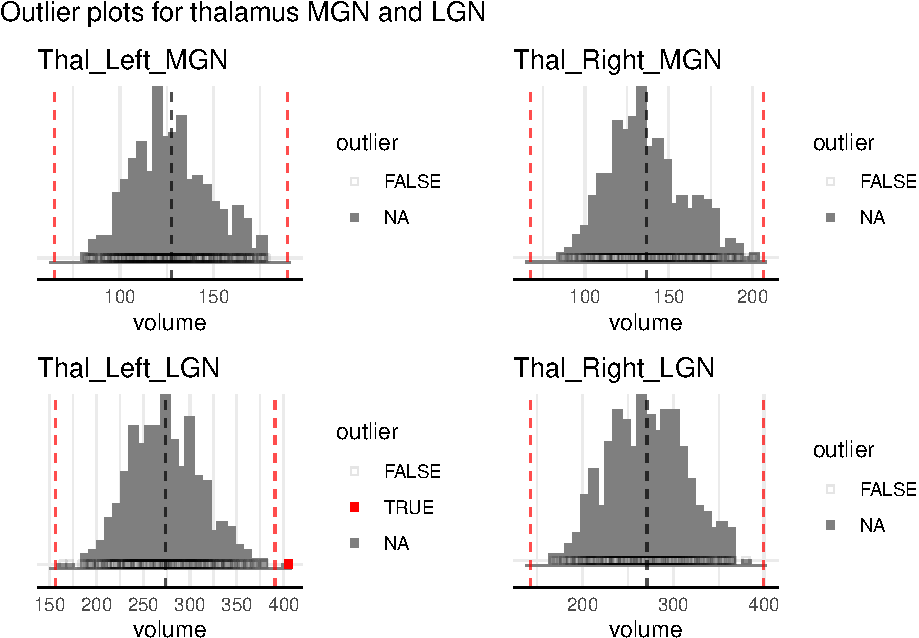
\includegraphics{22q_subcort_volumes_revised_files/figure-latex/unnamed-chunk-6-1.pdf}

\begin{Shaded}
\begin{Highlighting}[]
\CommentTok{\#ggsave(oplots\_out, file=file.path(project,"figures/review\_response/outlier\_plots.png"), device="png", width=7, height=4)}
\end{Highlighting}
\end{Shaded}

merge hemispheres by averaging whenever bilateral data are available

\begin{Shaded}
\begin{Highlighting}[]
\CommentTok{\# match left and right hemispheres in same row}
\NormalTok{sc\_long\_hemi }\OtherTok{\textless{}{-}}\NormalTok{ sc\_long\_inlier}
\NormalTok{sc\_long\_hemi}\SpecialCharTok{$}\NormalTok{bl\_region }\OtherTok{\textless{}{-}}\NormalTok{  sc\_long\_hemi}\SpecialCharTok{$}\NormalTok{variable }\SpecialCharTok{\%\textgreater{}\%} \FunctionTok{gsub}\NormalTok{(}\StringTok{"\_Left"}\NormalTok{,}\StringTok{""}\NormalTok{,.) }\SpecialCharTok{\%\textgreater{}\%} \FunctionTok{gsub}\NormalTok{(}\StringTok{"\_Right"}\NormalTok{,}\StringTok{""}\NormalTok{,.)}
\NormalTok{sc\_long\_hemi}\SpecialCharTok{$}\NormalTok{hemi }\OtherTok{\textless{}{-}}  \FunctionTok{str\_extract}\NormalTok{(}\AttributeTok{string=}\NormalTok{sc\_long\_hemi}\SpecialCharTok{$}\NormalTok{variable, }\AttributeTok{pattern=}\StringTok{"Left|Right"}\NormalTok{)}
\NormalTok{sc\_long\_hemi\_merged }\OtherTok{\textless{}{-}} \FunctionTok{merge}\NormalTok{(}\AttributeTok{x=}\FunctionTok{filter}\NormalTok{(sc\_long\_hemi, hemi}\SpecialCharTok{==}\StringTok{"Left"}\NormalTok{), }\AttributeTok{y=}\FunctionTok{filter}\NormalTok{(sc\_long\_hemi, hemi}\SpecialCharTok{==}\StringTok{"Right"}\NormalTok{), }\AttributeTok{by=}\FunctionTok{c}\NormalTok{(}\StringTok{"MRI\_S\_ID"}\NormalTok{,}\StringTok{"bl\_region"}\NormalTok{), }\AttributeTok{all.x=}\ConstantTok{TRUE}\NormalTok{, }\AttributeTok{all.y=}\ConstantTok{TRUE}\NormalTok{)}

\CommentTok{\# average left and right }
\NormalTok{sc\_long\_hemi\_avg }\OtherTok{\textless{}{-}}\NormalTok{ sc\_long\_hemi\_merged}
\NormalTok{sc\_long\_hemi\_avg}\SpecialCharTok{$}\NormalTok{bl\_volume }\OtherTok{\textless{}{-}} \ConstantTok{NA}
\ControlFlowTok{for}\NormalTok{(i }\ControlFlowTok{in} \DecValTok{1}\SpecialCharTok{:}\FunctionTok{nrow}\NormalTok{(sc\_long\_hemi\_avg))\{}
\NormalTok{  sc\_long\_hemi\_avg[i,}\StringTok{"bl\_volume"}\NormalTok{] }\OtherTok{\textless{}{-}} \FunctionTok{mean}\NormalTok{(}\AttributeTok{x=}\FunctionTok{c}\NormalTok{(sc\_long\_hemi\_avg[i,}\StringTok{"volume.x"}\NormalTok{], sc\_long\_hemi\_avg[i,}\StringTok{"volume.y"}\NormalTok{]), }\AttributeTok{na.rm=}\ConstantTok{TRUE}\NormalTok{)}
\NormalTok{\}}

\CommentTok{\# convert back to wide df for input to ComBat}
\FunctionTok{setDT}\NormalTok{(sc\_long\_hemi\_avg)}
\NormalTok{subcort\_bilat }\OtherTok{\textless{}{-}} \FunctionTok{dcast}\NormalTok{(sc\_long\_hemi\_avg, MRI\_S\_ID }\SpecialCharTok{\textasciitilde{}}\NormalTok{ bl\_region, }\AttributeTok{value.var=}\StringTok{"bl\_volume"}\NormalTok{)}
\end{Highlighting}
\end{Shaded}

lookup table for ROI info

\begin{Shaded}
\begin{Highlighting}[]
\CommentTok{\# read edited lookup table matching freesurfer names to full names}
\CommentTok{\#lut \textless{}{-} read.csv(file.path(project,"lut\_names\_thal\_hip\_amy\_match.txt"), header=TRUE)}
\NormalTok{lut }\OtherTok{\textless{}{-}} \FunctionTok{read.csv}\NormalTok{(}\FunctionTok{file.path}\NormalTok{(project,}\StringTok{"lut\_names\_thal\_hip\_amy\_match\_combine.csv"}\NormalTok{), }\AttributeTok{header=}\ConstantTok{TRUE}\NormalTok{)}
\NormalTok{lut}\SpecialCharTok{$}\NormalTok{region\_match }\OtherTok{\textless{}{-}} \FunctionTok{gsub}\NormalTok{(}\StringTok{"{-}"}\NormalTok{,}\StringTok{"\_"}\NormalTok{,lut}\SpecialCharTok{$}\NormalTok{region)}
\NormalTok{lut}\SpecialCharTok{$}\NormalTok{region\_match }\OtherTok{\textless{}{-}} \FunctionTok{gsub}\NormalTok{(}\StringTok{"}\SpecialCharTok{\textbackslash{}\textbackslash{}}\StringTok{("}\NormalTok{,}\StringTok{"\_"}\NormalTok{,lut}\SpecialCharTok{$}\NormalTok{region\_match)}
\NormalTok{lut}\SpecialCharTok{$}\NormalTok{region\_match }\OtherTok{\textless{}{-}} \FunctionTok{gsub}\NormalTok{(}\StringTok{"}\SpecialCharTok{\textbackslash{}\textbackslash{}}\StringTok{)"}\NormalTok{,}\StringTok{"\_"}\NormalTok{,lut}\SpecialCharTok{$}\NormalTok{region\_match)}

\CommentTok{\# edit lut for bilateral matching}
\NormalTok{lut\_bilat }\OtherTok{\textless{}{-}}\NormalTok{ lut}
\NormalTok{lut\_bilat}\SpecialCharTok{$}\NormalTok{bilat\_match }\OtherTok{\textless{}{-}}\NormalTok{ lut\_bilat}\SpecialCharTok{$}\NormalTok{region\_match }\SpecialCharTok{\%\textgreater{}\%} \FunctionTok{gsub}\NormalTok{(}\StringTok{"Right\_"}\NormalTok{,}\StringTok{""}\NormalTok{,.) }\SpecialCharTok{\%\textgreater{}\%} \FunctionTok{gsub}\NormalTok{(}\StringTok{"Left\_"}\NormalTok{,}\StringTok{""}\NormalTok{,.)}
\NormalTok{lut\_bilat}\SpecialCharTok{$}\NormalTok{bilat\_name }\OtherTok{\textless{}{-}}\NormalTok{ lut\_bilat}\SpecialCharTok{$}\NormalTok{Name }\SpecialCharTok{\%\textgreater{}\%} \FunctionTok{gsub}\NormalTok{(}\StringTok{"right"}\NormalTok{,}\StringTok{""}\NormalTok{,.) }\SpecialCharTok{\%\textgreater{}\%} \FunctionTok{gsub}\NormalTok{(}\StringTok{"left"}\NormalTok{,}\StringTok{""}\NormalTok{,.)}
\NormalTok{lut\_bilat\_n }\OtherTok{\textless{}{-}}\NormalTok{ lut\_bilat[,}\FunctionTok{c}\NormalTok{(}\StringTok{"bilat\_name"}\NormalTok{,}\StringTok{"bilat\_match"}\NormalTok{,}\StringTok{"Structure"}\NormalTok{)]}
\NormalTok{lut\_unique }\OtherTok{\textless{}{-}}\NormalTok{ lut\_bilat\_n[}\SpecialCharTok{!}\FunctionTok{duplicated}\NormalTok{(lut\_bilat\_n),]}
\NormalTok{lut\_unique}
\end{Highlighting}
\end{Shaded}

\begin{verbatim}
##                              bilat_name                  bilat_match
## 1                    lateral geniculate                          LGN
## 3                     medial geniculate                          MGN
## 5                     pulvinar inferior                          PuI
## 6                       pulvinar medial                          PuM
## 7            limitans (suprageniculate)                         L_Sg
## 8                ventral posterolateral                          VPL
## 9                          centromedian                           CM
## 10             ventral lateral anterior                          VLa
## 11                    pulvinar anterior                          PuA
## 12                   mediodorsal medial                          MDm
## 13                       parafascicular                           Pf
## 14                  ventral anterior mc                         VAmc
## 15                  mediodorsal lateral                          MDl
## 16                       central medial                          CeM
## 17                     ventral anterior                           VA
## 18            medial ventral (reuniens)                       MV_Re_
## 19                         ventromedial                           VM
## 20                      central lateral                           CL
## 21                     pulvinar lateral                          PuL
## 22                           paratenial                           Pt
## 23                        anteroventral                           AV
## 24                          paracentral                           Pc
## 25            ventral lateral posterior                          VLp
## 26                    lateral posterior                           LP
## 49                         laterodorsal                           LD
## 51                       whole thalamus               Whole_thalamus
## 53                     hippocampal tail             Hippocampal_tail
## 54                       subiculum body               subiculum_body
## 55                             CA1 body                     CA1_body
## 56                       subiculum head               subiculum_head
## 57                  hippocampal fissure          hippocampal_fissure
## 58                    presubiculum head            presubiculum_head
## 59                             CA1 head                     CA1_head
## 60                    presubiculum body            presubiculum_body
## 61                        parasubiculum                parasubiculum
## 62                 molecular layer head      molecular_layer_HP_head
## 63                 molecular layer body      molecular_layer_HP_body
## 64                        GC ML DG head                GC_ML_DG_head
## 65                             CA3 body                     CA3_body
## 66                        GC ML DG body                GC_ML_DG_body
## 67                             CA4 head                     CA4_head
## 68                             CA4 body                     CA4_body
## 69                              fimbria                      fimbria
## 70                             CA3 head                     CA3_head
## 71 hippocampal amygdala transition area                         HATA
## 72                    whole hippocampus            Whole_hippocampus
## 73               whole hippocampus body       Whole_hippocampal_body
## 74               whole hippocampus head       Whole_hippocampal_head
## 75                      lateral nucleus              Lateral_nucleus
## 76                        basal nucleus                Basal_nucleus
## 77              accessory basal nucleus      Accessory_Basal_nucleus
## 78             anterior amygdaloid area Anterior_amygdaloid_area_AAA
## 79                      central nucleus              Central_nucleus
## 80                       medial nucleus               Medial_nucleus
## 81                     cortical nucleus             Cortical_nucleus
## 82         corticoamygdaloid transition  Corticoamygdaloid_transitio
## 83                  paralaminar nucleus          Paralaminar_nucleus
## 84                       whole amygdala               Whole_amygdala
## 85                          mediodorsal                       MD_all
## 86                      ventral lateral                       VL_all
## 87                     ventral anterior                       VA_all
## 88                             pulvinar                      Pu_part
## 93                                  CA1                          CA1
## 94                                CA2/3                          CA3
## 95                                  CA4                          CA4
## 96                             GC ML DG                     GC_ML_DG
## 97                      molecular layer           molecular_layer_HP
## 98                         presubiculum                 presubiculum
## 99                            subiculum                    subiculum
##      Structure
## 1     thalamus
## 3     thalamus
## 5     thalamus
## 6     thalamus
## 7     thalamus
## 8     thalamus
## 9     thalamus
## 10    thalamus
## 11    thalamus
## 12    thalamus
## 13    thalamus
## 14    thalamus
## 15    thalamus
## 16    thalamus
## 17    thalamus
## 18    thalamus
## 19    thalamus
## 20    thalamus
## 21    thalamus
## 22    thalamus
## 23    thalamus
## 24    thalamus
## 25    thalamus
## 26    thalamus
## 49    thalamus
## 51    thalamus
## 53 hippocampus
## 54 hippocampus
## 55 hippocampus
## 56 hippocampus
## 57 hippocampus
## 58 hippocampus
## 59 hippocampus
## 60 hippocampus
## 61 hippocampus
## 62 hippocampus
## 63 hippocampus
## 64 hippocampus
## 65 hippocampus
## 66 hippocampus
## 67 hippocampus
## 68 hippocampus
## 69 hippocampus
## 70 hippocampus
## 71 hippocampus
## 72 hippocampus
## 73 hippocampus
## 74 hippocampus
## 75    amygdala
## 76    amygdala
## 77    amygdala
## 78    amygdala
## 79    amygdala
## 80    amygdala
## 81    amygdala
## 82    amygdala
## 83    amygdala
## 84    amygdala
## 85    thalamus
## 86    thalamus
## 87    thalamus
## 88    thalamus
## 93 hippocampus
## 94 hippocampus
## 95 hippocampus
## 96 hippocampus
## 97 hippocampus
## 98 hippocampus
## 99 hippocampus
\end{verbatim}

\begin{Shaded}
\begin{Highlighting}[]
\CommentTok{\# add eTIVnormed}
\NormalTok{lut\_unique }\OtherTok{\textless{}{-}} \FunctionTok{rbind}\NormalTok{(lut\_unique, }\FunctionTok{data.frame}\NormalTok{(}\AttributeTok{bilat\_name=}\StringTok{"total ICV"}\NormalTok{, }\AttributeTok{bilat\_match=}\StringTok{"eTIVnormed"}\NormalTok{, }\AttributeTok{Structure=}\StringTok{"whole brain"}\NormalTok{))}
\end{Highlighting}
\end{Shaded}

\hypertarget{load-sistat-data-and-get-lists-of-scans-to-use}{%
\subsection{load sistat data and get lists of scans to
use}\label{load-sistat-data-and-get-lists-of-scans-to-use}}

all sistat tables should be exported as CSVs into a single directory the
next several chunks deal with reading, cleaning and annotating the data
exported from sistat, and then age matching the hcs sample is younger
than del due to a large amount of very young hcs subjects. plan is to
match samples by using followup timepoints rather than baseline for some
younger participants, and dropping several older del subjects, and
younger hcs subjects (prioritizing dropping subjects with worse motion
stats when possible)

\begin{Shaded}
\begin{Highlighting}[]
\CommentTok{\# set location of directory with ucla sistat CSVs}
\NormalTok{csvdir\_ucla }\OtherTok{\textless{}{-}} \FunctionTok{file.path}\NormalTok{(project,}\StringTok{"demographics/ucla\_sistat"}\NormalTok{)}

\CommentTok{\# get list of files\_ucla in directory}
\NormalTok{files\_ucla }\OtherTok{\textless{}{-}} \FunctionTok{list.files}\NormalTok{(csvdir\_ucla)}
\NormalTok{fpaths }\OtherTok{\textless{}{-}} \FunctionTok{lapply}\NormalTok{(files\_ucla, }\ControlFlowTok{function}\NormalTok{(file) }\FunctionTok{paste}\NormalTok{(csvdir\_ucla,file,}\AttributeTok{sep=}\StringTok{"/"}\NormalTok{))}

\CommentTok{\# clean names}
\NormalTok{fnames }\OtherTok{\textless{}{-}} \FunctionTok{gsub}\NormalTok{(}\StringTok{".csv"}\NormalTok{,}\StringTok{""}\NormalTok{,files\_ucla)}
\NormalTok{fnames }\OtherTok{\textless{}{-}} \FunctionTok{gsub}\NormalTok{(}\StringTok{"Re22Q\_"}\NormalTok{,}\StringTok{""}\NormalTok{,fnames)}
\NormalTok{fnames }\OtherTok{\textless{}{-}} \FunctionTok{gsub}\NormalTok{(}\StringTok{"Form\_"}\NormalTok{,}\StringTok{""}\NormalTok{,fnames)}
\NormalTok{fnames }\OtherTok{\textless{}{-}} \FunctionTok{gsub}\NormalTok{(}\StringTok{"Qry\_"}\NormalTok{,}\StringTok{""}\NormalTok{,fnames)}

\CommentTok{\# read all, set to na: "{-}9999", "{-}9998","." }
\NormalTok{input\_all\_ucla }\OtherTok{\textless{}{-}} \FunctionTok{lapply}\NormalTok{(fpaths, read.csv, }\AttributeTok{header=}\NormalTok{T, }\AttributeTok{na.strings=}\FunctionTok{c}\NormalTok{(}\StringTok{"."}\NormalTok{,}\StringTok{"{-}9999"}\NormalTok{,}\StringTok{"{-}9998"}\NormalTok{), }\AttributeTok{strip.white=}\NormalTok{T, }\AttributeTok{sep=}\StringTok{","}\NormalTok{)}
\FunctionTok{names}\NormalTok{(input\_all\_ucla) }\OtherTok{\textless{}{-}}\NormalTok{ fnames}
\NormalTok{df\_all\_ucla }\OtherTok{\textless{}{-}} \FunctionTok{lapply}\NormalTok{(input\_all\_ucla, }\ControlFlowTok{function}\NormalTok{(x) }\FunctionTok{data.frame}\NormalTok{(x))}

\CommentTok{\# get demo\_mri }
\NormalTok{ucla\_demo }\OtherTok{\textless{}{-}}\NormalTok{ df\_all\_ucla}\SpecialCharTok{$}\NormalTok{demo\_mri}

\CommentTok{\# remove "FAMILY MEMBER" designation from subject identity}
\NormalTok{ucla\_demo}\SpecialCharTok{$}\NormalTok{SUBJECT\_IDENTITY }\OtherTok{\textless{}{-}}\NormalTok{ ucla\_demo}\SpecialCharTok{$}\NormalTok{SUBJECT\_IDENTITY }\SpecialCharTok{\%\textgreater{}\%} \FunctionTok{sub}\NormalTok{(}\StringTok{"FAMILY MEMBER"}\NormalTok{,}\StringTok{""}\NormalTok{,.) }\SpecialCharTok{\%\textgreater{}\%} \FunctionTok{sub}\NormalTok{(}\StringTok{","}\NormalTok{,}\StringTok{""}\NormalTok{,.) }\SpecialCharTok{\%\textgreater{}\%} \FunctionTok{trimws}\NormalTok{(}\AttributeTok{which=}\StringTok{"both"}\NormalTok{) }\SpecialCharTok{\%\textgreater{}\%}\NormalTok{ as.factor}
\CommentTok{\# change sex coding from 0/1 to F/M and set to factor}
\NormalTok{ucla\_demo}\SpecialCharTok{$}\NormalTok{SEX }\OtherTok{\textless{}{-}} \FunctionTok{factor}\NormalTok{(ucla\_demo}\SpecialCharTok{$}\NormalTok{SEX,}\AttributeTok{levels=}\FunctionTok{c}\NormalTok{(}\DecValTok{0}\NormalTok{,}\DecValTok{1}\NormalTok{),}\AttributeTok{labels=}\FunctionTok{c}\NormalTok{(}\StringTok{"F"}\NormalTok{,}\StringTok{"M"}\NormalTok{))}
\end{Highlighting}
\end{Shaded}

read temporary csv with several subjects not yet in sistat

\begin{Shaded}
\begin{Highlighting}[]
\CommentTok{\# }\AlertTok{TODO}\CommentTok{: this chunk is temporary until sistat is updated }
\CommentTok{\# }\AlertTok{TODO}\CommentTok{: note: q\_0526 sex was "na" in original sheet, changed to M because combat can\textquotesingle{}t have NAs}
\CommentTok{\# read new data}
\NormalTok{temp\_demo }\OtherTok{\textless{}{-}} \FunctionTok{read\_xlsx}\NormalTok{(}\FunctionTok{file.path}\NormalTok{(project,}\StringTok{"demographics/temporary/sMRI\_demo\_info\_forCharlie.xlsx"}\NormalTok{), }\AttributeTok{col\_names=}\ConstantTok{TRUE}\NormalTok{,}\AttributeTok{na=}\StringTok{""}\NormalTok{,}\AttributeTok{trim\_ws =} \ConstantTok{TRUE}\NormalTok{)}

\CommentTok{\# make empty demographics data frame to add new data to}
\NormalTok{demo\_add }\OtherTok{\textless{}{-}}\NormalTok{ ucla\_demo[}\DecValTok{1}\SpecialCharTok{:}\FunctionTok{nrow}\NormalTok{(temp\_demo),]}
\NormalTok{demo\_add[,] }\OtherTok{\textless{}{-}} \ConstantTok{NA}
\NormalTok{demo\_add}\SpecialCharTok{$}\NormalTok{SUBJECTID }\OtherTok{\textless{}{-}}\NormalTok{ temp\_demo}\SpecialCharTok{$}\StringTok{\textasciigrave{}}\AttributeTok{Subject ID}\StringTok{\textasciigrave{}}
\NormalTok{demo\_add}\SpecialCharTok{$}\NormalTok{SUBJECT\_IDENTITY }\OtherTok{\textless{}{-}}\NormalTok{ temp\_demo}\SpecialCharTok{$}\NormalTok{Diagnosis}
\NormalTok{demo\_add}\SpecialCharTok{$}\NormalTok{MRI\_S\_ID }\OtherTok{\textless{}{-}}\NormalTok{ temp\_demo}\SpecialCharTok{$}\StringTok{\textasciigrave{}}\AttributeTok{MRI ID}\StringTok{\textasciigrave{}}
\NormalTok{demo\_add}\SpecialCharTok{$}\NormalTok{SEX }\OtherTok{\textless{}{-}} \FunctionTok{as.factor}\NormalTok{(temp\_demo}\SpecialCharTok{$}\NormalTok{Sex)}
\NormalTok{demo\_add}\SpecialCharTok{$}\NormalTok{AGE }\OtherTok{\textless{}{-}}\NormalTok{ temp\_demo}\SpecialCharTok{$}\NormalTok{Age}
\NormalTok{demo\_add}\SpecialCharTok{$}\NormalTok{AGEMONTH }\OtherTok{\textless{}{-}}\NormalTok{ temp\_demo}\SpecialCharTok{$}\NormalTok{Age}\SpecialCharTok{*}\DecValTok{12}
\NormalTok{demo\_add}\SpecialCharTok{$}\NormalTok{CONVERTEDVISITNUM }\OtherTok{\textless{}{-}} \DecValTok{2}

\CommentTok{\# append to ucla demo}
\NormalTok{ucla\_demo }\OtherTok{\textless{}{-}} \FunctionTok{rbind}\NormalTok{(ucla\_demo,demo\_add)}
\end{Highlighting}
\end{Shaded}

continue regular steps

\begin{Shaded}
\begin{Highlighting}[]
\CommentTok{\# manually fix missing sex for Q\_0381\_09102019}
\CommentTok{\# }\AlertTok{TODO}\CommentTok{: fix in sistat and re{-}export}
\NormalTok{ucla\_demo[}\FunctionTok{which}\NormalTok{(ucla\_demo}\SpecialCharTok{$}\NormalTok{MRI\_S\_ID }\SpecialCharTok{==} \StringTok{"Q\_0381\_09102019"}\NormalTok{),}\StringTok{"SEX"}\NormalTok{] }\OtherTok{\textless{}{-}} \StringTok{"F"}

\CommentTok{\# set race=NA to 7 (unknown)}
\NormalTok{ucla\_demo}\SpecialCharTok{$}\NormalTok{RACE[}\FunctionTok{is.na}\NormalTok{(ucla\_demo}\SpecialCharTok{$}\NormalTok{RACE)] }\OtherTok{\textless{}{-}} \DecValTok{7}
\CommentTok{\# set race as factor 1=American Indian/Alaska Native; 2=Asian; 3=Native Hawaiian/Pacific Islander; 4=Black or African American; 5=White; 6=Multiple; 7=Unknown}
\NormalTok{ucla\_demo}\SpecialCharTok{$}\NormalTok{RACE }\OtherTok{\textless{}{-}} \FunctionTok{factor}\NormalTok{(ucla\_demo}\SpecialCharTok{$}\NormalTok{RACE,}\AttributeTok{levels=}\FunctionTok{c}\NormalTok{(}\DecValTok{1}\SpecialCharTok{:}\DecValTok{7}\NormalTok{),}\AttributeTok{labels=}\FunctionTok{c}\NormalTok{(}\StringTok{"1\_Native\_American"}\NormalTok{,}\StringTok{"2\_Asian"}\NormalTok{,}\StringTok{"3\_Pacific\_Island"}\NormalTok{,}\StringTok{"4\_Black"}\NormalTok{,}\StringTok{"5\_White"}\NormalTok{,}\StringTok{"6\_Multiple"}\NormalTok{,}\StringTok{"7\_Unknown"}\NormalTok{))}
\CommentTok{\# ethnicity as factor with 0=N 1=Y}
\NormalTok{ucla\_demo}\SpecialCharTok{$}\NormalTok{HISPANIC[}\FunctionTok{is.na}\NormalTok{(ucla\_demo}\SpecialCharTok{$}\NormalTok{HISPANIC)] }\OtherTok{\textless{}{-}} \StringTok{"Unknown"}
\NormalTok{ucla\_demo}\SpecialCharTok{$}\NormalTok{HISPANIC }\OtherTok{\textless{}{-}} \FunctionTok{factor}\NormalTok{(ucla\_demo}\SpecialCharTok{$}\NormalTok{HISPANIC,}\AttributeTok{levels=}\FunctionTok{c}\NormalTok{(}\DecValTok{0}\NormalTok{,}\DecValTok{1}\NormalTok{,}\StringTok{"Unknown"}\NormalTok{),}\AttributeTok{labels=}\FunctionTok{c}\NormalTok{(}\StringTok{"N"}\NormalTok{,}\StringTok{"Y"}\NormalTok{,}\StringTok{"Unknown"}\NormalTok{))}
\CommentTok{\# get more accurate age with AGEMONTH/12}
\NormalTok{ucla\_demo}\SpecialCharTok{$}\NormalTok{AGE }\OtherTok{\textless{}{-}} \FunctionTok{as.numeric}\NormalTok{(ucla\_demo}\SpecialCharTok{$}\NormalTok{AGEMONTH)}\SpecialCharTok{/}\DecValTok{12} 

\CommentTok{\# subset to used scans}
\NormalTok{ucla\_demo }\OtherTok{\textless{}{-}} \FunctionTok{filter}\NormalTok{(ucla\_demo, MRI\_S\_ID }\SpecialCharTok{\%in\%}\NormalTok{ subcort\_all}\SpecialCharTok{$}\NormalTok{MRI\_S\_ID)}

\CommentTok{\# function to add column to code timepoints relative to sample used (i.e. if visit 1 and 1.12 missing, then 1.24 is baseline)}
\CommentTok{\# trio/prisma coded as T/P{-}visit\_n where T{-}1 would be the subject\textquotesingle{}s first trio scan and P{-}1 the first prisma, P{-}2 the second...}
\CommentTok{\# function should be applied to the indicies of rows (r) in a subset of demo\_mri}
\NormalTok{gettp }\OtherTok{\textless{}{-}} \ControlFlowTok{function}\NormalTok{(r, df)\{}
\NormalTok{  sub }\OtherTok{\textless{}{-}}\NormalTok{ df}\SpecialCharTok{$}\NormalTok{SUBJECTID[[r]]}
\NormalTok{  visit }\OtherTok{\textless{}{-}}\NormalTok{ df}\SpecialCharTok{$}\NormalTok{CONVERTEDVISITNUM[[r]]}
\NormalTok{  all\_visits }\OtherTok{\textless{}{-}}\NormalTok{ df}\SpecialCharTok{$}\NormalTok{CONVERTEDVISITNUM[}\FunctionTok{which}\NormalTok{(df}\SpecialCharTok{$}\NormalTok{SUBJECTID }\SpecialCharTok{==}\NormalTok{ sub)] }\SpecialCharTok{\%\textgreater{}\%}\NormalTok{ sort}
\NormalTok{  n\_visits }\OtherTok{\textless{}{-}} \FunctionTok{length}\NormalTok{(all\_visits)}
\NormalTok{  nt\_visits }\OtherTok{\textless{}{-}}\FunctionTok{length}\NormalTok{(}\FunctionTok{which}\NormalTok{(all\_visits }\SpecialCharTok{\textless{}} \DecValTok{2}\NormalTok{))}
\NormalTok{  np\_visits }\OtherTok{\textless{}{-}} \FunctionTok{length}\NormalTok{(}\FunctionTok{which}\NormalTok{(all\_visits }\SpecialCharTok{\textgreater{}=} \DecValTok{2}\NormalTok{))}
\NormalTok{  visit\_index }\OtherTok{\textless{}{-}} \FunctionTok{which}\NormalTok{(all\_visits }\SpecialCharTok{==}\NormalTok{ visit)}
  \ControlFlowTok{if}\NormalTok{ (visit }\SpecialCharTok{\textless{}} \DecValTok{2}\NormalTok{)\{}
\NormalTok{    label}\OtherTok{=}\FunctionTok{paste}\NormalTok{(}\StringTok{"T{-}"}\NormalTok{,visit\_index,}\AttributeTok{sep=}\StringTok{""}\NormalTok{)}
\NormalTok{  \}}\ControlFlowTok{else} \ControlFlowTok{if}\NormalTok{ (visit }\SpecialCharTok{\textgreater{}=} \DecValTok{2}\NormalTok{)\{}
\NormalTok{    p\_visits }\OtherTok{\textless{}{-}}\NormalTok{ all\_visits[}\FunctionTok{which}\NormalTok{(all\_visits }\SpecialCharTok{\textgreater{}=} \DecValTok{2}\NormalTok{)] }\SpecialCharTok{\%\textgreater{}\%}\NormalTok{ sort}
\NormalTok{    p\_visit\_index }\OtherTok{\textless{}{-}} \FunctionTok{which}\NormalTok{(p\_visits }\SpecialCharTok{==}\NormalTok{ visit)}
\NormalTok{    label}\OtherTok{=}\FunctionTok{paste}\NormalTok{(}\StringTok{"P{-}"}\NormalTok{,p\_visit\_index,}\AttributeTok{sep=}\StringTok{""}\NormalTok{)}
\NormalTok{  \}}
  \FunctionTok{return}\NormalTok{(}\FunctionTok{c}\NormalTok{(sub,visit,label,n\_visits,nt\_visits,np\_visits,visit\_index))}
\NormalTok{\}}

\CommentTok{\# get timepoints}
\NormalTok{timepoints }\OtherTok{\textless{}{-}} \FunctionTok{lapply}\NormalTok{(}\DecValTok{1}\SpecialCharTok{:}\FunctionTok{nrow}\NormalTok{(ucla\_demo),}\ControlFlowTok{function}\NormalTok{(r) }\FunctionTok{gettp}\NormalTok{(r,ucla\_demo)) }\SpecialCharTok{\%\textgreater{}\%} \FunctionTok{do.call}\NormalTok{(rbind,.) }\SpecialCharTok{\%\textgreater{}\%}\NormalTok{ as.data.frame}
\FunctionTok{colnames}\NormalTok{(timepoints) }\OtherTok{\textless{}{-}} \FunctionTok{c}\NormalTok{(}\StringTok{"SUBJECTID"}\NormalTok{,}\StringTok{"CONVERTEDVISITNUM"}\NormalTok{,}\StringTok{"converted\_timepoint"}\NormalTok{,}\StringTok{"n\_timepoints"}\NormalTok{,}\StringTok{"n\_trio"}\NormalTok{,}\StringTok{"n\_prisma"}\NormalTok{,}\StringTok{"visit\_index"}\NormalTok{)}
\NormalTok{ucla\_demo\_tp }\OtherTok{\textless{}{-}} \FunctionTok{cbind}\NormalTok{(ucla\_demo,timepoints[,}\DecValTok{3}\SpecialCharTok{:}\DecValTok{7}\NormalTok{])}
\NormalTok{ucla\_demo\_tp}\SpecialCharTok{$}\NormalTok{visit\_index }\SpecialCharTok{\%\textless{}\textgreater{}\%}\NormalTok{ as.factor}

\CommentTok{\# subset to under max age limit (45 years old)}
\NormalTok{ucla\_demo\_tp\_agelim }\OtherTok{\textless{}{-}} \FunctionTok{filter}\NormalTok{(ucla\_demo\_tp, ucla\_demo\_tp}\SpecialCharTok{$}\NormalTok{AGE }\SpecialCharTok{\textless{}} \DecValTok{50}\NormalTok{)}
\CommentTok{\#ucla\_demo\_tp\_agelim \textless{}{-} filter(ucla\_demo\_tp, ucla\_demo\_tp$AGE \textless{} 44)}

\CommentTok{\# subset to hcs del}
\CommentTok{\#ucla\_demo\_hcs\_del \textless{}{-} ucla\_demo\_tp\_agelim \%\textgreater{}\% filter(SUBJECT\_IDENTITY=="CONTROL" | SUBJECT\_IDENTITY =="PATIENT{-}DEL")}

\CommentTok{\# remove unused factor levels}
\NormalTok{ucla\_demo\_tp\_agelim }\SpecialCharTok{\%\textless{}\textgreater{}\%}\NormalTok{ droplevels}
\end{Highlighting}
\end{Shaded}

All timepoints, demographics summary

\begin{Shaded}
\begin{Highlighting}[]
\NormalTok{demo\_summary }\OtherTok{\textless{}{-}} \FunctionTok{CreateTableOne}\NormalTok{(}\AttributeTok{data=}\NormalTok{ucla\_demo\_tp\_agelim,}\AttributeTok{vars=}\FunctionTok{c}\NormalTok{(}\StringTok{"AGE"}\NormalTok{,}\StringTok{"SEX"}\NormalTok{),}\AttributeTok{strata=}\StringTok{"SUBJECT\_IDENTITY"}\NormalTok{,}\AttributeTok{addOverall=}\NormalTok{F)}
\FunctionTok{print}\NormalTok{(demo\_summary, }\AttributeTok{showAllLevels=}\NormalTok{T)}
\end{Highlighting}
\end{Shaded}

\begin{verbatim}
##                  Stratified by SUBJECT_IDENTITY
##                   level CONTROL       PATIENT-DEL   PATIENT-DUP   p      test
##   n                       130           191            64                    
##   AGE (mean (SD))       14.74 (6.68)  17.17 (7.78)  17.88 (12.40)  0.014     
##   SEX (%)         F        64 (49.2)    111 (58.1)     26 (40.6)   0.037     
##                   M        66 (50.8)     80 (41.9)     38 (59.4)
\end{verbatim}

\begin{Shaded}
\begin{Highlighting}[]
\CommentTok{\#print(demo\_summary, showAllLevels=F)}
\end{Highlighting}
\end{Shaded}

under 35, demographics summary

\begin{Shaded}
\begin{Highlighting}[]
\NormalTok{demo\_summary\_young }\OtherTok{\textless{}{-}} \FunctionTok{CreateTableOne}\NormalTok{(}\AttributeTok{data=}\FunctionTok{filter}\NormalTok{(ucla\_demo\_tp\_agelim, AGE }\SpecialCharTok{\textless{}} \DecValTok{35}\NormalTok{),}\AttributeTok{vars=}\FunctionTok{c}\NormalTok{(}\StringTok{"AGE"}\NormalTok{,}\StringTok{"SEX"}\NormalTok{),}\AttributeTok{strata=}\StringTok{"SUBJECT\_IDENTITY"}\NormalTok{,}\AttributeTok{addOverall=}\NormalTok{F)}
\FunctionTok{print}\NormalTok{(demo\_summary\_young, }\AttributeTok{showAllLevels=}\NormalTok{T)}
\end{Highlighting}
\end{Shaded}

\begin{verbatim}
##                  Stratified by SUBJECT_IDENTITY
##                   level CONTROL       PATIENT-DEL   PATIENT-DUP   p      test
##   n                       128           182            54                    
##   AGE (mean (SD))       14.30 (5.69)  16.06 (6.08)  13.25 (6.33)   0.003     
##   SEX (%)         F        62 (48.4)    106 (58.2)     19 (35.2)   0.008     
##                   M        66 (51.6)     76 (41.8)     35 (64.8)
\end{verbatim}

\begin{Shaded}
\begin{Highlighting}[]
\CommentTok{\#print(demo\_summary, showAllLevels=F)}
\end{Highlighting}
\end{Shaded}

Baseline summary

\begin{Shaded}
\begin{Highlighting}[]
\NormalTok{demo\_summary\_bl }\OtherTok{\textless{}{-}} \FunctionTok{CreateTableOne}\NormalTok{(}\AttributeTok{data=}\FunctionTok{filter}\NormalTok{(ucla\_demo\_tp\_agelim, visit\_index }\SpecialCharTok{==} \DecValTok{1}\NormalTok{),}\AttributeTok{vars=}\FunctionTok{c}\NormalTok{(}\StringTok{"AGE"}\NormalTok{,}\StringTok{"SEX"}\NormalTok{),}\AttributeTok{strata=}\StringTok{"SUBJECT\_IDENTITY"}\NormalTok{,}\AttributeTok{addOverall=}\NormalTok{F)}
\FunctionTok{print}\NormalTok{(demo\_summary\_bl)}
\end{Highlighting}
\end{Shaded}

\begin{verbatim}
##                  Stratified by SUBJECT_IDENTITY
##                   CONTROL       PATIENT-DEL   PATIENT-DUP   p      test
##   n                  80            96            37                    
##   AGE (mean (SD)) 14.89 (7.34)  15.52 (7.62)  17.83 (13.50)  0.240     
##   SEX = M (%)        39 (48.8)     45 (46.9)     20 (54.1)   0.759
\end{verbatim}

Age waterfall plot

\begin{Shaded}
\begin{Highlighting}[]
\NormalTok{ucla\_demo\_waterfall }\OtherTok{\textless{}{-}}\NormalTok{ ucla\_demo\_tp\_agelim}
\NormalTok{ucla\_demo\_waterfall}\SpecialCharTok{$}\NormalTok{Scanner }\OtherTok{\textless{}{-}} \FunctionTok{gsub}\NormalTok{(}\StringTok{"{-}[0{-}9]"}\NormalTok{,}\StringTok{""}\NormalTok{,ucla\_demo\_waterfall}\SpecialCharTok{$}\NormalTok{converted\_timepoint)}
\NormalTok{ucla\_demo\_waterfall}\SpecialCharTok{$}\NormalTok{Scanner }\SpecialCharTok{\%\textless{}\textgreater{}\%} \FunctionTok{gsub}\NormalTok{(}\StringTok{"T"}\NormalTok{,}\StringTok{"trio"}\NormalTok{,.)}
\NormalTok{ucla\_demo\_waterfall}\SpecialCharTok{$}\NormalTok{Scanner }\SpecialCharTok{\%\textless{}\textgreater{}\%} \FunctionTok{gsub}\NormalTok{(}\StringTok{"P"}\NormalTok{,}\StringTok{"prisma"}\NormalTok{,.)}
\NormalTok{ucla\_demo\_waterfall}\SpecialCharTok{$}\NormalTok{Group }\OtherTok{\textless{}{-}}\NormalTok{ ucla\_demo\_waterfall}\SpecialCharTok{$}\NormalTok{SUBJECT\_IDENTITY}
\CommentTok{\# get age at timepoint 1 for every row}
\NormalTok{ucla\_demo\_waterfall}\SpecialCharTok{$}\NormalTok{age1 }\OtherTok{\textless{}{-}} \FunctionTok{lapply}\NormalTok{(ucla\_demo\_waterfall}\SpecialCharTok{$}\NormalTok{SUBJECTID, }\ControlFlowTok{function}\NormalTok{(i) }\FunctionTok{min}\NormalTok{(}\FunctionTok{filter}\NormalTok{(ucla\_demo\_waterfall, SUBJECTID}\SpecialCharTok{==}\NormalTok{i)}\SpecialCharTok{$}\NormalTok{AGEMONTH)) }\SpecialCharTok{\%\textgreater{}\%} \FunctionTok{do.call}\NormalTok{(rbind,.)}

\CommentTok{\#waterfall \textless{}{-} ggplot(ucla\_demo\_waterfall, aes(x=(AGEMONTH/12), y=reorder(SUBJECTID, AGEMONTH),color=Group, fill=Group)) +}
\NormalTok{waterfall }\OtherTok{\textless{}{-}} \FunctionTok{ggplot}\NormalTok{(ucla\_demo\_waterfall, }\FunctionTok{aes}\NormalTok{(}\AttributeTok{x=}\NormalTok{(AGEMONTH}\SpecialCharTok{/}\DecValTok{12}\NormalTok{), }\AttributeTok{y=}\FunctionTok{as.factor}\NormalTok{(age1) ,}\AttributeTok{color=}\NormalTok{Group, }\AttributeTok{fill=}\NormalTok{Group)) }\SpecialCharTok{+}
  \FunctionTok{geom\_point}\NormalTok{(}\FunctionTok{aes}\NormalTok{(}\AttributeTok{shape=}\NormalTok{Scanner), }\AttributeTok{color=}\StringTok{"black"}\NormalTok{,}\AttributeTok{alpha=}\FloatTok{0.7}\NormalTok{) }\SpecialCharTok{+} 
  \FunctionTok{scale\_shape\_manual}\NormalTok{(}\AttributeTok{values =} \FunctionTok{c}\NormalTok{(}\DecValTok{24}\NormalTok{,}\DecValTok{21}\NormalTok{)) }\SpecialCharTok{+} 
  \FunctionTok{theme\_classic}\NormalTok{() }\SpecialCharTok{+} 
  \CommentTok{\#theme(text=element\_text(family="Arial"))+}
  \FunctionTok{theme}\NormalTok{(}\AttributeTok{axis.text.y=}\FunctionTok{element\_blank}\NormalTok{(), }\AttributeTok{axis.ticks.x=}\FunctionTok{element\_blank}\NormalTok{(),}\AttributeTok{axis.ticks.y=}\FunctionTok{element\_blank}\NormalTok{()) }\SpecialCharTok{+} 
  \FunctionTok{geom\_line}\NormalTok{(}\FunctionTok{aes}\NormalTok{(}\AttributeTok{group=}\NormalTok{SUBJECTID,}\AttributeTok{color=}\NormalTok{SUBJECT\_IDENTITY),}\AttributeTok{alpha=}\FloatTok{0.7}\NormalTok{) }\SpecialCharTok{+}
  \FunctionTok{scale\_fill\_manual}\NormalTok{(}\AttributeTok{values =} \FunctionTok{c}\NormalTok{(}\StringTok{"CONTROL"} \OtherTok{=} \FunctionTok{viridis}\NormalTok{(}\DecValTok{3}\NormalTok{)[}\DecValTok{2}\NormalTok{], }\StringTok{"PATIENT{-}DEL"} \OtherTok{=} \FunctionTok{viridis}\NormalTok{(}\DecValTok{3}\NormalTok{)[}\DecValTok{1}\NormalTok{], }\StringTok{"PATIENT{-}DUP"} \OtherTok{=} \FunctionTok{viridis}\NormalTok{(}\DecValTok{3}\NormalTok{)[}\DecValTok{3}\NormalTok{]), }\AttributeTok{labels =} \FunctionTok{c}\NormalTok{(}\StringTok{"Control"}\NormalTok{, }\StringTok{"22qDel"}\NormalTok{, }\StringTok{"22qDup"}\NormalTok{)) }\SpecialCharTok{+}
  \FunctionTok{scale\_color\_manual}\NormalTok{(}\AttributeTok{values =} \FunctionTok{c}\NormalTok{(}\StringTok{"CONTROL"} \OtherTok{=} \FunctionTok{viridis}\NormalTok{(}\DecValTok{3}\NormalTok{)[}\DecValTok{2}\NormalTok{], }\StringTok{"PATIENT{-}DEL"} \OtherTok{=} \FunctionTok{viridis}\NormalTok{(}\DecValTok{3}\NormalTok{)[}\DecValTok{1}\NormalTok{], }\StringTok{"PATIENT{-}DUP"} \OtherTok{=} \FunctionTok{viridis}\NormalTok{(}\DecValTok{3}\NormalTok{)[}\DecValTok{3}\NormalTok{]), }\AttributeTok{labels =} \FunctionTok{c}\NormalTok{(}\StringTok{"Control"}\NormalTok{, }\StringTok{"22qDel"}\NormalTok{, }\StringTok{"22qDup"}\NormalTok{)) }\SpecialCharTok{+}
  \CommentTok{\#guides(color  = guide\_legend(order =1, override.aes = list(color=c(viridis(3)[2],viridis(3)[1],viridis(3)[3]))))+}
  \FunctionTok{guides}\NormalTok{(}\AttributeTok{fill  =} \FunctionTok{guide\_legend}\NormalTok{(}\AttributeTok{order =} \DecValTok{1}\NormalTok{, }\AttributeTok{override.aes =} \FunctionTok{list}\NormalTok{(}\AttributeTok{shape=}\DecValTok{21}\NormalTok{, }\AttributeTok{size=}\FloatTok{2.4}\NormalTok{,}\AttributeTok{alpha=}\FloatTok{0.9}\NormalTok{, }\AttributeTok{fill=}\FunctionTok{c}\NormalTok{(}\FunctionTok{viridis}\NormalTok{(}\DecValTok{3}\NormalTok{)[}\DecValTok{2}\NormalTok{],}\FunctionTok{viridis}\NormalTok{(}\DecValTok{3}\NormalTok{)[}\DecValTok{1}\NormalTok{],}\FunctionTok{viridis}\NormalTok{(}\DecValTok{3}\NormalTok{)[}\DecValTok{3}\NormalTok{]))),}
         \AttributeTok{color =} \FunctionTok{guide\_legend}\NormalTok{(}\AttributeTok{order=}\DecValTok{1}\NormalTok{),}
         \AttributeTok{shape =} \FunctionTok{guide\_legend}\NormalTok{(}\AttributeTok{order =} \DecValTok{2}\NormalTok{, }\AttributeTok{override.aes =} \FunctionTok{list}\NormalTok{(}\AttributeTok{size=}\FloatTok{2.5}\NormalTok{)))}\SpecialCharTok{+}
  \FunctionTok{ylab}\NormalTok{(}\StringTok{"Individual"}\NormalTok{) }\SpecialCharTok{+}
  \FunctionTok{xlab}\NormalTok{(}\StringTok{"Age"}\NormalTok{) }\SpecialCharTok{+}
  \FunctionTok{xlim}\NormalTok{(}\DecValTok{5}\NormalTok{,}\DecValTok{50}\NormalTok{)}\SpecialCharTok{+}
  \FunctionTok{ggtitle}\NormalTok{(}\StringTok{"Age at scan"}\NormalTok{)}\SpecialCharTok{+}
  \FunctionTok{coord\_cartesian}\NormalTok{(}\AttributeTok{clip =} \StringTok{"off"}\NormalTok{)}

\NormalTok{waterfall}
\end{Highlighting}
\end{Shaded}

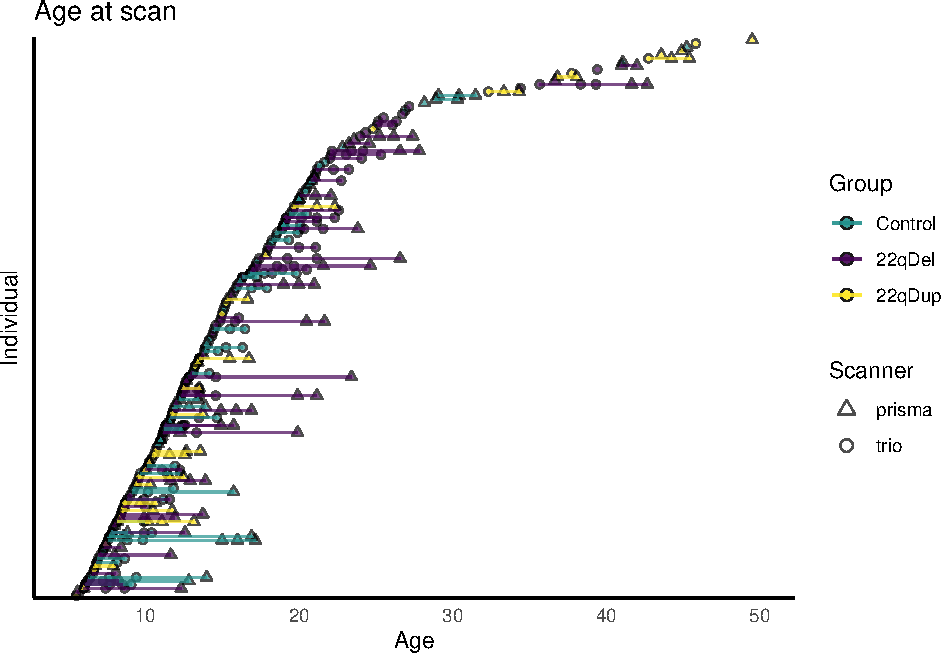
\includegraphics{22q_subcort_volumes_revised_files/figure-latex/unnamed-chunk-15-1.pdf}

\begin{Shaded}
\begin{Highlighting}[]
\CommentTok{\#ggsave(plot=waterfall, filename=file.path(project,"figures/demographics/waterfall\_subcort\_age.pdf"), width=6, height=6, device = "pdf")}
\CommentTok{\#ggsave(plot=waterfall, filename=file.path(project,"figures/demographics/waterfall\_subcort\_age.png"), width=6, height=6, device = "png")}
\end{Highlighting}
\end{Shaded}

\hypertarget{harmonize-sites}{%
\subsection{Harmonize sites}\label{harmonize-sites}}

merge imaging with demographics

\begin{Shaded}
\begin{Highlighting}[]
\CommentTok{\# add site column}
\NormalTok{ucla\_demo\_tp\_agelim}\SpecialCharTok{$}\NormalTok{site }\OtherTok{\textless{}{-}} \FunctionTok{gsub}\NormalTok{(}\StringTok{"*{-}[0{-}9]"}\NormalTok{,}\StringTok{""}\NormalTok{,ucla\_demo\_tp\_agelim}\SpecialCharTok{$}\NormalTok{converted\_timepoint)}

\CommentTok{\# merge subcort\_all with demo}
\CommentTok{\#demo\_sc \textless{}{-} merge(x=ucla\_demo\_tp\_agelim, y=subcort\_all, by="MRI\_S\_ID", all.x=TRUE)}
\NormalTok{demo\_sc }\OtherTok{\textless{}{-}} \FunctionTok{merge}\NormalTok{(}\AttributeTok{x=}\NormalTok{ucla\_demo\_tp\_agelim, }\AttributeTok{y=}\NormalTok{subcort\_bilat, }\AttributeTok{by=}\StringTok{"MRI\_S\_ID"}\NormalTok{, }\AttributeTok{all.x=}\ConstantTok{TRUE}\NormalTok{)}

\CommentTok{\# merge with eTIV}
\NormalTok{demo\_sc }\OtherTok{\textless{}{-}} \FunctionTok{merge}\NormalTok{(}\AttributeTok{x=}\NormalTok{demo\_sc, }\AttributeTok{y=}\NormalTok{etiv, }\AttributeTok{by=}\StringTok{"MRI\_S\_ID"}\NormalTok{)}
\NormalTok{demo\_sc}\SpecialCharTok{$}\NormalTok{eTIVscaled }\OtherTok{\textless{}{-}}\NormalTok{ demo\_sc}\SpecialCharTok{$}\NormalTok{eTIV}\SpecialCharTok{/}\DecValTok{1000000}

\CommentTok{\# make numeric gene dosage column from SUBJECT\_IDENTITY}
\NormalTok{demo\_sc}\SpecialCharTok{$}\NormalTok{gene\_dosage }\OtherTok{\textless{}{-}}\NormalTok{ demo\_sc}\SpecialCharTok{$}\NormalTok{SUBJECT\_IDENTITY }\SpecialCharTok{\%\textgreater{}\%} \FunctionTok{gsub}\NormalTok{(}\StringTok{"PATIENT{-}DEL"}\NormalTok{,}\StringTok{"1"}\NormalTok{,.) }\SpecialCharTok{\%\textgreater{}\%} \FunctionTok{gsub}\NormalTok{(}\StringTok{"CONTROL"}\NormalTok{,}\StringTok{"2"}\NormalTok{,.) }\SpecialCharTok{\%\textgreater{}\%} \FunctionTok{gsub}\NormalTok{(}\StringTok{"PATIENT{-}DUP"}\NormalTok{,}\StringTok{"3"}\NormalTok{,.) }\SpecialCharTok{\%\textgreater{}\%}\NormalTok{ as.numeric}

\CommentTok{\# add Age\^{}2}
\CommentTok{\# add age\^{}2}
\NormalTok{demo\_sc}\SpecialCharTok{$}\NormalTok{AGE2 }\OtherTok{\textless{}{-}}\NormalTok{ demo\_sc}\SpecialCharTok{$}\NormalTok{AGE}\SpecialCharTok{\^{}}\DecValTok{2}

\CommentTok{\# update feature names to bilateral columns}
\NormalTok{sc\_names }\OtherTok{\textless{}{-}} \FunctionTok{names}\NormalTok{(subcort\_bilat)[}\FunctionTok{which}\NormalTok{(}\FunctionTok{names}\NormalTok{(subcort\_bilat) }\SpecialCharTok{!=} \StringTok{"MRI\_S\_ID"}\NormalTok{)]}
\end{Highlighting}
\end{Shaded}

impute outliers and excluded data (ComBat can't have NAs in input)

\begin{Shaded}
\begin{Highlighting}[]
\CommentTok{\# list of thalamus regions}
\CommentTok{\#thal\_names\_final \textless{}{-} names(subcort\_all)[grep("Thal",names(subcort\_all))]}
\NormalTok{thal\_names\_final }\OtherTok{\textless{}{-}} \FunctionTok{names}\NormalTok{(subcort\_bilat)[}\FunctionTok{grep}\NormalTok{(}\StringTok{"Thal"}\NormalTok{,}\FunctionTok{names}\NormalTok{(subcort\_bilat))]}
\CommentTok{\# data frame with MRI\_S\_ID and region names to remove}
\CommentTok{\# first get all the thalamus ROIs for the subjects with whole thal excluded}
\NormalTok{remove\_thal }\OtherTok{\textless{}{-}} \FunctionTok{lapply}\NormalTok{(thal\_exclude, }\ControlFlowTok{function}\NormalTok{(n) }\FunctionTok{data.frame}\NormalTok{(}\AttributeTok{MRI\_S\_ID =}\NormalTok{ n, }\AttributeTok{variable=}\NormalTok{thal\_names\_final)) }\SpecialCharTok{\%\textgreater{}\%} \FunctionTok{do.call}\NormalTok{(rbind,.)}
\CommentTok{\# and add that to the subjects/regions in out\_filter}
\CommentTok{\#sparse\_remove \textless{}{-} rbind(out\_filter[,c("MRI\_S\_ID","variable")], remove\_thal)}

\CommentTok{\# add to all subjects/regions with NAs in subcort\_bilat}
\CommentTok{\# initialize empty vectors to store row and column names}
\NormalTok{row\_names\_true }\OtherTok{\textless{}{-}} \FunctionTok{character}\NormalTok{(}\DecValTok{0}\NormalTok{)}
\NormalTok{col\_names\_true }\OtherTok{\textless{}{-}} \FunctionTok{character}\NormalTok{(}\DecValTok{0}\NormalTok{)}
\CommentTok{\# prepare input}
\NormalTok{sc\_rn }\OtherTok{\textless{}{-}} \FunctionTok{is.na}\NormalTok{(}\FunctionTok{as.data.frame}\NormalTok{(subcort\_bilat)[,sc\_names])}
\FunctionTok{rownames}\NormalTok{(sc\_rn) }\OtherTok{\textless{}{-}}\NormalTok{ subcort\_bilat}\SpecialCharTok{$}\NormalTok{MRI\_S\_ID}
\CommentTok{\# loop through the data frame to find TRUE values}
\ControlFlowTok{for}\NormalTok{ (i }\ControlFlowTok{in} \DecValTok{1}\SpecialCharTok{:}\FunctionTok{nrow}\NormalTok{(sc\_rn)) \{}
  \ControlFlowTok{for}\NormalTok{ (j }\ControlFlowTok{in} \DecValTok{1}\SpecialCharTok{:}\FunctionTok{ncol}\NormalTok{(sc\_rn)) \{}
    \ControlFlowTok{if}\NormalTok{ (sc\_rn[i,j]) \{}
\NormalTok{      row\_names\_true }\OtherTok{\textless{}{-}} \FunctionTok{c}\NormalTok{(row\_names\_true, }\FunctionTok{rownames}\NormalTok{(sc\_rn)[i])}
\NormalTok{      col\_names\_true }\OtherTok{\textless{}{-}} \FunctionTok{c}\NormalTok{(col\_names\_true, }\FunctionTok{colnames}\NormalTok{(sc\_rn)[j])}
\NormalTok{    \}}
\NormalTok{  \}}
\NormalTok{\}}

\CommentTok{\# Create a data frame from the vectors}
\NormalTok{bilat\_remove }\OtherTok{\textless{}{-}} \FunctionTok{data.frame}\NormalTok{(}\AttributeTok{MRI\_S\_ID =}\NormalTok{ row\_names\_true, }\AttributeTok{variable =}\NormalTok{ col\_names\_true)}
\NormalTok{sparse\_remove }\OtherTok{\textless{}{-}} \FunctionTok{rbind}\NormalTok{(bilat\_remove, remove\_thal)}

\CommentTok{\# add site and gene dosage from demo\_sc}
\NormalTok{sparse\_remove }\OtherTok{\textless{}{-}} \FunctionTok{merge}\NormalTok{(}\AttributeTok{x=}\NormalTok{sparse\_remove, }\AttributeTok{y=}\NormalTok{demo\_sc[,}\FunctionTok{c}\NormalTok{(}\StringTok{"MRI\_S\_ID"}\NormalTok{,}\StringTok{"site"}\NormalTok{,}\StringTok{"gene\_dosage"}\NormalTok{)], }\AttributeTok{by=}\StringTok{"MRI\_S\_ID"}\NormalTok{)}

\CommentTok{\# replace with overall mean for that structure}
\NormalTok{demo\_sc\_impute }\OtherTok{\textless{}{-}}\NormalTok{ demo\_sc}
\ControlFlowTok{for}\NormalTok{ (i }\ControlFlowTok{in} \DecValTok{1}\SpecialCharTok{:}\FunctionTok{nrow}\NormalTok{(sparse\_remove))\{}
\NormalTok{  sesh }\OtherTok{\textless{}{-}} \FunctionTok{as.character}\NormalTok{(sparse\_remove[i,}\StringTok{"MRI\_S\_ID"}\NormalTok{])}
\NormalTok{  roi }\OtherTok{\textless{}{-}} \FunctionTok{as.character}\NormalTok{(sparse\_remove[i,}\StringTok{"variable"}\NormalTok{])}
\NormalTok{  s }\OtherTok{\textless{}{-}} \FunctionTok{as.character}\NormalTok{(sparse\_remove[i,}\StringTok{"site"}\NormalTok{])}
\NormalTok{  gd }\OtherTok{\textless{}{-}} \FunctionTok{as.numeric}\NormalTok{(sparse\_remove[i,}\StringTok{"gene\_dosage"}\NormalTok{])}
  \CommentTok{\#print(paste(sesh,roi,s,gd), sep=", ")}
  \CommentTok{\# first, set to NA in demo\_sc\_impute}
\NormalTok{  demo\_sc\_impute[}\FunctionTok{which}\NormalTok{(demo\_sc\_impute}\SpecialCharTok{$}\NormalTok{MRI\_S\_ID}\SpecialCharTok{==}\NormalTok{sesh),roi] }\OtherTok{\textless{}{-}} \ConstantTok{NA}
  \CommentTok{\# then for that ROI, get mean for the same diagnostic group and scanner as current subject}
\NormalTok{  demo\_filter }\OtherTok{\textless{}{-}} \FunctionTok{filter}\NormalTok{(demo\_sc\_impute, gene\_dosage }\SpecialCharTok{==}\NormalTok{ gd }\SpecialCharTok{\&}\NormalTok{ site }\SpecialCharTok{==}\NormalTok{ s)}
\NormalTok{  roi\_mean }\OtherTok{\textless{}{-}} \FunctionTok{mean}\NormalTok{(demo\_filter[,roi],}\AttributeTok{na.rm=}\ConstantTok{TRUE}\NormalTok{)}
  \CommentTok{\#print(roi\_mean)}
  \CommentTok{\# replace with mean}
\NormalTok{  demo\_sc\_impute[}\FunctionTok{which}\NormalTok{(demo\_sc\_impute}\SpecialCharTok{$}\NormalTok{MRI\_S\_ID}\SpecialCharTok{==}\NormalTok{sesh),roi] }\OtherTok{\textless{}{-}}\NormalTok{ roi\_mean}
\NormalTok{\}}
\end{Highlighting}
\end{Shaded}

run longComBat

\begin{Shaded}
\begin{Highlighting}[]
\CommentTok{\# set up longCombat variables}
\CommentTok{\# formula should match fixed effects in your subsequent analysis}
\CommentTok{\# subject id coded as random effect by (1|subject id variable)}
\CommentTok{\#demovars \textless{}{-} c("MRI\_S\_ID","SUBJECTID","site","gene\_dosage","AGE","SEX","eTIVscaled","visit\_index")}
\NormalTok{demovars }\OtherTok{\textless{}{-}} \FunctionTok{c}\NormalTok{(}\StringTok{"MRI\_S\_ID"}\NormalTok{,}\StringTok{"SUBJECTID"}\NormalTok{,}\StringTok{"site"}\NormalTok{,}\StringTok{"gene\_dosage"}\NormalTok{,}\StringTok{"AGE"}\NormalTok{,}\StringTok{"AGE2"}\NormalTok{,}\StringTok{"SEX"}\NormalTok{,}\StringTok{"eTIVscaled"}\NormalTok{,}\StringTok{"visit\_index"}\NormalTok{)}
\NormalTok{features }\OtherTok{\textless{}{-}}\NormalTok{ sc\_names}
\NormalTok{idvar }\OtherTok{\textless{}{-}} \StringTok{\textquotesingle{}MRI\_S\_ID\textquotesingle{}}
\NormalTok{batchvar }\OtherTok{\textless{}{-}} \StringTok{\textquotesingle{}site\textquotesingle{}}
\NormalTok{timevar }\OtherTok{\textless{}{-}} \StringTok{\textquotesingle{}visit\_index\textquotesingle{}}
\NormalTok{formula }\OtherTok{\textless{}{-}} \StringTok{\textquotesingle{}gene\_dosage + AGE + AGE2 + SEX + eTIVscaled\textquotesingle{}}
\NormalTok{ranef }\OtherTok{\textless{}{-}} \StringTok{\textquotesingle{}(1|SUBJECTID)\textquotesingle{}}

\CommentTok{\# make data frame with columns for each variable in the model}
\CommentTok{\# one column for each variable in your formula as well as one column for each neuroimaging feature}
\CommentTok{\# input df should not have any unused columns or package will error}
\CommentTok{\# one row per unique scan}
\NormalTok{combat\_input}\OtherTok{\textless{}{-}}\NormalTok{ demo\_sc\_impute[,}\FunctionTok{c}\NormalTok{(demovars,features)]}

\CommentTok{\# run longCombat}
\NormalTok{sc\_vol\_combat }\OtherTok{\textless{}{-}} \FunctionTok{longCombat}\NormalTok{(}\AttributeTok{data=}\NormalTok{combat\_input, }\AttributeTok{idvar=}\NormalTok{idvar, }\AttributeTok{timevar=}\NormalTok{timevar, }\AttributeTok{batchvar=}\NormalTok{batchvar, }\AttributeTok{features=}\NormalTok{features, }\AttributeTok{formula=}\NormalTok{formula, }\AttributeTok{ranef=}\NormalTok{ranef, }\AttributeTok{verbose=}\ConstantTok{FALSE}\NormalTok{)}

\CommentTok{\# get the harmonized data}
\NormalTok{sc\_vol\_combat\_data }\OtherTok{\textless{}{-}}\NormalTok{ sc\_vol\_combat}\SpecialCharTok{$}\NormalTok{data\_combat}

\CommentTok{\# merge combat back with original}
\NormalTok{demo\_combat }\OtherTok{\textless{}{-}} \FunctionTok{merge}\NormalTok{(}\AttributeTok{x=}\NormalTok{demo\_sc, }\AttributeTok{y=}\NormalTok{sc\_vol\_combat\_data, }\AttributeTok{by=}\FunctionTok{c}\NormalTok{(}\StringTok{"MRI\_S\_ID"}\NormalTok{,}\StringTok{"visit\_index"}\NormalTok{,}\StringTok{"site"}\NormalTok{))}
\end{Highlighting}
\end{Shaded}

\hypertarget{gene-dosage-and-age-models}{%
\subsection{gene dosage and age
models}\label{gene-dosage-and-age-models}}

first, set up data frame

\begin{Shaded}
\begin{Highlighting}[]
\CommentTok{\# get names of combat features}
\NormalTok{sc\_names\_combat }\OtherTok{\textless{}{-}} \FunctionTok{paste0}\NormalTok{(sc\_names,}\StringTok{".combat"}\NormalTok{)}

\CommentTok{\# set outliers to NA after combat}
\NormalTok{demo\_combat\_na }\OtherTok{\textless{}{-}}\NormalTok{ demo\_combat}
\ControlFlowTok{for}\NormalTok{ (i }\ControlFlowTok{in} \DecValTok{1}\SpecialCharTok{:}\FunctionTok{nrow}\NormalTok{(sparse\_remove))\{}
\NormalTok{  sesh }\OtherTok{\textless{}{-}} \FunctionTok{as.character}\NormalTok{(sparse\_remove[i,}\StringTok{"MRI\_S\_ID"}\NormalTok{])}
\NormalTok{  roi }\OtherTok{\textless{}{-}} \FunctionTok{as.character}\NormalTok{(sparse\_remove[i,}\StringTok{"variable"}\NormalTok{])}
\NormalTok{  demo\_combat\_na[}\FunctionTok{which}\NormalTok{(demo\_combat\_na}\SpecialCharTok{$}\NormalTok{MRI\_S\_ID}\SpecialCharTok{==}\NormalTok{sesh),}\FunctionTok{paste0}\NormalTok{(roi,}\StringTok{".combat"}\NormalTok{)] }\OtherTok{\textless{}{-}} \ConstantTok{NA}
\NormalTok{\}}

\CommentTok{\# save demo\_combat}
\CommentTok{\#write.csv(demo\_combat\_na, file=file.path(project,"22q\_subcort\_vols\_combat\_na.csv"), quote=TRUE, row.names = FALSE)}
\end{Highlighting}
\end{Shaded}

normalize based on control group mean and SD to get standardized betas

\begin{Shaded}
\begin{Highlighting}[]
\CommentTok{\# names for normed columns}
\NormalTok{sc\_names\_normed }\OtherTok{\textless{}{-}} \FunctionTok{paste0}\NormalTok{(sc\_names\_combat, }\StringTok{".norm"}\NormalTok{)}

\CommentTok{\# for every region, get mean and SD for control group}
\NormalTok{norm\_name\_match }\OtherTok{\textless{}{-}} \FunctionTok{data.frame}\NormalTok{(}\AttributeTok{combat=}\NormalTok{sc\_names\_combat, }\AttributeTok{normed=}\NormalTok{sc\_names\_normed, }\AttributeTok{control\_mean=}\ConstantTok{NA}\NormalTok{, }\AttributeTok{control\_sd=}\ConstantTok{NA}\NormalTok{)}
\ControlFlowTok{for}\NormalTok{ (r }\ControlFlowTok{in} \DecValTok{1}\SpecialCharTok{:}\FunctionTok{nrow}\NormalTok{(norm\_name\_match))\{}
\NormalTok{  region }\OtherTok{\textless{}{-}}\NormalTok{ norm\_name\_match[r,}\StringTok{"combat"}\NormalTok{]}
\NormalTok{  control\_dat }\OtherTok{\textless{}{-}} \FunctionTok{filter}\NormalTok{(demo\_combat\_na, SUBJECT\_IDENTITY}\SpecialCharTok{==}\StringTok{"CONTROL"}\NormalTok{)[,region]}
\NormalTok{  norm\_name\_match[r,}\StringTok{"control\_mean"}\NormalTok{] }\OtherTok{\textless{}{-}} \FunctionTok{mean}\NormalTok{(control\_dat, }\AttributeTok{na.rm=}\ConstantTok{TRUE}\NormalTok{)}
\NormalTok{  norm\_name\_match[r,}\StringTok{"control\_sd"}\NormalTok{] }\OtherTok{\textless{}{-}} \FunctionTok{sd}\NormalTok{(control\_dat, }\AttributeTok{na.rm=}\ConstantTok{TRUE}\NormalTok{)}
\NormalTok{\}}

\CommentTok{\# df to hold normed data}
\NormalTok{demo\_combat\_normed }\OtherTok{\textless{}{-}}\NormalTok{ demo\_combat\_na}
\NormalTok{demo\_combat\_normed[r,sc\_names\_normed] }\OtherTok{\textless{}{-}} \ConstantTok{NA}

\CommentTok{\# for every region in each subject, normalize based on control mean and SD}
\ControlFlowTok{for}\NormalTok{ (r }\ControlFlowTok{in} \DecValTok{1}\SpecialCharTok{:}\FunctionTok{nrow}\NormalTok{(demo\_combat\_normed))\{ }
  \ControlFlowTok{for}\NormalTok{ (c }\ControlFlowTok{in} \DecValTok{1}\SpecialCharTok{:}\FunctionTok{nrow}\NormalTok{(norm\_name\_match))\{}
    \CommentTok{\# get column names and control stats for a given region}
\NormalTok{    combat\_name }\OtherTok{\textless{}{-}}\NormalTok{ norm\_name\_match[c,}\StringTok{"combat"}\NormalTok{]}
\NormalTok{    normed\_name }\OtherTok{\textless{}{-}}\NormalTok{ norm\_name\_match[c,}\StringTok{"normed"}\NormalTok{]}
\NormalTok{    control\_mean }\OtherTok{\textless{}{-}}\NormalTok{ norm\_name\_match[c,}\StringTok{"control\_mean"}\NormalTok{]}
\NormalTok{    control\_sd }\OtherTok{\textless{}{-}}\NormalTok{ norm\_name\_match[c,}\StringTok{"control\_sd"}\NormalTok{]}
    \CommentTok{\# get the pre{-}normed combat{-}adjusted value}
\NormalTok{    combat\_val }\OtherTok{\textless{}{-}}\NormalTok{ demo\_combat\_normed[r,combat\_name]}
    \CommentTok{\# if not NA, normalize based on control stats }
    \ControlFlowTok{if}\NormalTok{(}\FunctionTok{is.na}\NormalTok{(combat\_val))\{}
\NormalTok{      normed\_val }\OtherTok{\textless{}{-}} \ConstantTok{NA}
\NormalTok{    \}}\ControlFlowTok{else}\NormalTok{\{}
\NormalTok{      normed\_val }\OtherTok{\textless{}{-}}\NormalTok{ (combat\_val }\SpecialCharTok{{-}}\NormalTok{ control\_mean)}\SpecialCharTok{/}\NormalTok{control\_sd}
\NormalTok{    \}}
    \CommentTok{\# store normed value}
\NormalTok{    demo\_combat\_normed[r,normed\_name] }\OtherTok{\textless{}{-}}\NormalTok{ normed\_val}
\NormalTok{  \}}
\NormalTok{\}}

\CommentTok{\# normalize ICV}
\NormalTok{td\_mean\_icv }\OtherTok{\textless{}{-}} \FunctionTok{filter}\NormalTok{(demo\_combat\_normed, gene\_dosage}\SpecialCharTok{==}\DecValTok{2}\NormalTok{)}\SpecialCharTok{$}\NormalTok{eTIV }\SpecialCharTok{\%\textgreater{}\%}\NormalTok{ mean}
\NormalTok{td\_sd\_icv }\OtherTok{\textless{}{-}} \FunctionTok{filter}\NormalTok{(demo\_combat\_normed, gene\_dosage}\SpecialCharTok{==}\DecValTok{2}\NormalTok{)}\SpecialCharTok{$}\NormalTok{eTIV }\SpecialCharTok{\%\textgreater{}\%}\NormalTok{ sd}
\NormalTok{demo\_combat\_normed}\SpecialCharTok{$}\NormalTok{eTIVnormed }\OtherTok{\textless{}{-}}\NormalTok{ (demo\_combat\_normed}\SpecialCharTok{$}\NormalTok{eTIV }\SpecialCharTok{{-}}\NormalTok{ td\_mean\_icv)}\SpecialCharTok{/}\NormalTok{td\_sd\_icv}
\end{Highlighting}
\end{Shaded}

longitudinal demo table

\begin{Shaded}
\begin{Highlighting}[]
\CommentTok{\#dir \textless{}{-} "/Users/charlie/Dropbox/PhD/bearden\_lab/22q/analyses/striatum\_thalamus\_fc"}

\CommentTok{\# get variables from demo\_mri}
\NormalTok{df\_demo }\OtherTok{\textless{}{-}}\NormalTok{ demo\_combat\_na}

\DocumentationTok{\#\#\# hand}
\CommentTok{\# get handedness item scores coded in sistat as 1=L, 2=R, 3=either, 0=no experience}
\NormalTok{edin }\OtherTok{\textless{}{-}}\NormalTok{ df\_all\_ucla}\SpecialCharTok{$}\NormalTok{edin[,}\FunctionTok{c}\NormalTok{(}\StringTok{"SUBJECTID"}\NormalTok{,}\StringTok{"CONVERTEDVISITNUM"}\NormalTok{,}\StringTok{"EDIN1"}\NormalTok{,}\StringTok{"EDIN2"}\NormalTok{,}\StringTok{"EDIN3"}\NormalTok{,}\StringTok{"EDIN4"}\NormalTok{,}\StringTok{"EDIN5"}\NormalTok{,}\StringTok{"EDIN6"}\NormalTok{,}\StringTok{"EDIN7"}\NormalTok{,}\StringTok{"EDIN8"}\NormalTok{,}\StringTok{"EDIN9"}\NormalTok{,}\StringTok{"EDIN10"}\NormalTok{)]}
\CommentTok{\# function to get total edinburgh score and handedness}
\CommentTok{\# formula is 100*(R{-}L)/(R+L). score \textless{} {-}40 means left handed, score \textgreater{} 40 right handed}
\CommentTok{\# if more than 2 items NA then score is NA}
\NormalTok{get\_hand }\OtherTok{\textless{}{-}} \ControlFlowTok{function}\NormalTok{(edin)\{}
\NormalTok{  sub }\OtherTok{\textless{}{-}}\NormalTok{ edin[}\FunctionTok{c}\NormalTok{(}\StringTok{"SUBJECTID"}\NormalTok{)]}
\NormalTok{  visit }\OtherTok{\textless{}{-}}\NormalTok{ edin[}\FunctionTok{c}\NormalTok{(}\StringTok{"CONVERTEDVISITNUM"}\NormalTok{)]}
\NormalTok{  scores }\OtherTok{\textless{}{-}}\NormalTok{ edin[}\FunctionTok{c}\NormalTok{(}\StringTok{"EDIN1"}\NormalTok{,}\StringTok{"EDIN2"}\NormalTok{,}\StringTok{"EDIN3"}\NormalTok{,}\StringTok{"EDIN4"}\NormalTok{,}\StringTok{"EDIN5"}\NormalTok{,}\StringTok{"EDIN6"}\NormalTok{,}\StringTok{"EDIN7"}\NormalTok{,}\StringTok{"EDIN8"}\NormalTok{,}\StringTok{"EDIN9"}\NormalTok{,}\StringTok{"EDIN10"}\NormalTok{)]}
\NormalTok{  l }\OtherTok{\textless{}{-}} \FunctionTok{sum}\NormalTok{(scores }\SpecialCharTok{==} \DecValTok{1}\NormalTok{, }\AttributeTok{na.rm=}\ConstantTok{TRUE}\NormalTok{)}
\NormalTok{  r }\OtherTok{\textless{}{-}} \FunctionTok{sum}\NormalTok{(scores }\SpecialCharTok{==} \DecValTok{2}\NormalTok{, }\AttributeTok{na.rm=}\ConstantTok{TRUE}\NormalTok{)}
\NormalTok{  na }\OtherTok{\textless{}{-}} \FunctionTok{sum}\NormalTok{(}\FunctionTok{is.na}\NormalTok{(scores))}
  \ControlFlowTok{if}\NormalTok{ (na }\SpecialCharTok{\textless{}} \DecValTok{3}\NormalTok{)\{}
\NormalTok{    score }\OtherTok{\textless{}{-}} \DecValTok{10}\SpecialCharTok{*}\NormalTok{(r}\SpecialCharTok{{-}}\NormalTok{l)}
\NormalTok{  \}}
  \ControlFlowTok{if}\NormalTok{ (na }\SpecialCharTok{\textgreater{}} \DecValTok{2}\NormalTok{)\{}
\NormalTok{    hand }\OtherTok{\textless{}{-}} \ConstantTok{NA}
\NormalTok{    score }\OtherTok{\textless{}{-}} \ConstantTok{NA}
\NormalTok{  \}}\ControlFlowTok{else} \ControlFlowTok{if}\NormalTok{(score }\SpecialCharTok{\textgreater{}} \DecValTok{40}\NormalTok{)\{}
\NormalTok{    hand }\OtherTok{\textless{}{-}}\StringTok{"R"}
\NormalTok{  \}}\ControlFlowTok{else} \ControlFlowTok{if}\NormalTok{ (score }\SpecialCharTok{\textless{}} \SpecialCharTok{{-}}\DecValTok{40}\NormalTok{)\{}
\NormalTok{    hand }\OtherTok{\textless{}{-}} \StringTok{"L"}
\NormalTok{  \}}\ControlFlowTok{else} \ControlFlowTok{if}\NormalTok{ (score }\SpecialCharTok{\textgreater{}=} \SpecialCharTok{{-}}\DecValTok{40} \SpecialCharTok{\&}\NormalTok{ score }\SpecialCharTok{\textless{}=} \DecValTok{40}\NormalTok{) \{}
\NormalTok{    hand }\OtherTok{\textless{}{-}} \StringTok{"A"}
\NormalTok{  \}}\ControlFlowTok{else}\NormalTok{\{}
\NormalTok{    hand }\OtherTok{\textless{}{-}} \ConstantTok{NA}
\NormalTok{  \}}
\NormalTok{  output }\OtherTok{\textless{}{-}} \FunctionTok{cbind}\NormalTok{(sub,visit,score,hand) }\SpecialCharTok{\%\textgreater{}\%}\NormalTok{ as.data.frame}
  \FunctionTok{colnames}\NormalTok{(output) }\OtherTok{\textless{}{-}} \FunctionTok{c}\NormalTok{(}\StringTok{"SUBJECTID"}\NormalTok{,}\StringTok{"CONVERTEDVISITNUM"}\NormalTok{,}\StringTok{"hand\_score"}\NormalTok{,}\StringTok{"hand"}\NormalTok{)}
  \FunctionTok{return}\NormalTok{(output)}
\NormalTok{\}}
\CommentTok{\# get handedness}
\NormalTok{edin\_result }\OtherTok{\textless{}{-}} \FunctionTok{lapply}\NormalTok{(}\DecValTok{1}\SpecialCharTok{:}\FunctionTok{nrow}\NormalTok{(edin), }\ControlFlowTok{function}\NormalTok{(r) }\FunctionTok{get\_hand}\NormalTok{(edin[r,])) }\SpecialCharTok{\%\textgreater{}\%} \FunctionTok{do.call}\NormalTok{(rbind,.) }\SpecialCharTok{\%\textgreater{}\%}\NormalTok{ as.data.frame}

\CommentTok{\# merge handedness with demo table}
\NormalTok{df\_demo }\OtherTok{\textless{}{-}} \FunctionTok{merge}\NormalTok{(}\AttributeTok{x=}\NormalTok{df\_demo, }\AttributeTok{y=}\NormalTok{edin\_result[}\FunctionTok{c}\NormalTok{(}\StringTok{"SUBJECTID"}\NormalTok{,}\StringTok{"CONVERTEDVISITNUM"}\NormalTok{,}\StringTok{"hand"}\NormalTok{)], }\AttributeTok{by=}\FunctionTok{c}\NormalTok{(}\StringTok{"SUBJECTID"}\NormalTok{,}\StringTok{"CONVERTEDVISITNUM"}\NormalTok{), }\AttributeTok{all.x=}\NormalTok{T)}

\CommentTok{\# manually fix a few subjects\textquotesingle{} handedness}
\CommentTok{\#q\_0017="A"}
\NormalTok{df\_demo[}\FunctionTok{which}\NormalTok{(df\_demo}\SpecialCharTok{$}\NormalTok{SUBJECTID }\SpecialCharTok{==} \StringTok{"q\_0017"}\NormalTok{),}\StringTok{"hand"}\NormalTok{] }\OtherTok{\textless{}{-}} \StringTok{"A"}
\CommentTok{\#q\_0263="R"}
\NormalTok{df\_demo[}\FunctionTok{which}\NormalTok{(df\_demo}\SpecialCharTok{$}\NormalTok{SUBJECTID }\SpecialCharTok{==} \StringTok{"q\_0263"}\NormalTok{),}\StringTok{"hand"}\NormalTok{] }\OtherTok{\textless{}{-}} \StringTok{"R"}
\CommentTok{\#q\_0331="R"}
\NormalTok{df\_demo[}\FunctionTok{which}\NormalTok{(df\_demo}\SpecialCharTok{$}\NormalTok{SUBJECTID }\SpecialCharTok{==} \StringTok{"q\_0331"}\NormalTok{),}\StringTok{"hand"}\NormalTok{] }\OtherTok{\textless{}{-}} \StringTok{"R"}

\DocumentationTok{\#\#\# psych dx}
\CommentTok{\# first get SCID columns with Dx (currently only using patient Dx not collateral)}
\NormalTok{scid\_dx\_all }\OtherTok{\textless{}{-}}\NormalTok{ df\_all\_ucla}\SpecialCharTok{$}\NormalTok{SCID[,}\FunctionTok{c}\NormalTok{(}\StringTok{"PATCODE1"}\NormalTok{,}\StringTok{"PATCODE2"}\NormalTok{,}\StringTok{"PATCODE3"}\NormalTok{,}\StringTok{"PATCODE4"}\NormalTok{,}\StringTok{"PATCODE5"}\NormalTok{,}\StringTok{"PATCODE6"}\NormalTok{,}\StringTok{"PATCODE7"}\NormalTok{,}\StringTok{"PATCODE8"}\NormalTok{)]}

\CommentTok{\# get list of unique dx entries}
\NormalTok{dx\_unique }\OtherTok{\textless{}{-}}\NormalTok{ scid\_dx\_all }\SpecialCharTok{\%\textgreater{}\%}\NormalTok{ as.matrix }\SpecialCharTok{\%\textgreater{}\%}\NormalTok{ as.vector }\SpecialCharTok{\%\textgreater{}\%}\NormalTok{ sort }\SpecialCharTok{\%\textgreater{}\%}\NormalTok{ unique}

\CommentTok{\# create matching key between unique dx and dx groups for demographics table}
\CommentTok{\# first save dx\_unique as csv}
\CommentTok{\#write.table(dx\_unique, file=file.path(csvdir\_ucla,"scid\_unique\_dx.csv"), row.names=F, col.names=F)}
\CommentTok{\# then manually edit csv so that column 2 contains the dx group for each specific dx. save edited csv as scid\_unique\_dx\_matching.csv}
\CommentTok{\# dx group categories based on DSM{-}5 https://www.psychiatry.org/File\%20Library/Psychiatrists/Practice/DSM/APA\_DSM{-}5{-}Contents.pdf}
\CommentTok{\# Notes: leave second column blank for non{-}psych dx (eg Crohn\textquotesingle{}s), code single{-}episode MDD in full remission as depressive\_disorder\_past, all other MDD as depressive\_disorder}
\CommentTok{\# read matching table back in }
\NormalTok{dx\_unique\_matching }\OtherTok{\textless{}{-}} \FunctionTok{read.csv}\NormalTok{(}\AttributeTok{file=}\FunctionTok{file.path}\NormalTok{(project,}\StringTok{"demographics/scid\_unique\_dx\_matching.csv"}\NormalTok{), }\AttributeTok{header=}\NormalTok{F)}

\CommentTok{\# function to take scid patient codes 1{-}8 for a subject and output binary y/n for each dx in dx\_groups based on dx\_unique\_matching}
\CommentTok{\# should be applied to rows of the scid data frame}
\NormalTok{get\_general\_dx\_scid }\OtherTok{\textless{}{-}} \ControlFlowTok{function}\NormalTok{(scid\_row,dx\_matching)\{}
  \CommentTok{\# get subject id and visit columns}
\NormalTok{  id\_cols }\OtherTok{\textless{}{-}}\NormalTok{ scid\_row[}\FunctionTok{c}\NormalTok{(}\StringTok{"SUBJECTID"}\NormalTok{,}\StringTok{"CONVERTEDVISITNUM"}\NormalTok{)]}
  \CommentTok{\# get list of all unique dx groups in matching key}
\NormalTok{  dx\_groups }\OtherTok{\textless{}{-}}\NormalTok{ dx\_matching[,}\DecValTok{2}\NormalTok{] }\SpecialCharTok{\%\textgreater{}\%}\NormalTok{ sort }\SpecialCharTok{\%\textgreater{}\%}\NormalTok{ unique}
\NormalTok{  dx\_groups }\OtherTok{\textless{}{-}}\NormalTok{ dx\_groups[dx\_groups }\SpecialCharTok{!=} \StringTok{""}\NormalTok{]}
  \CommentTok{\# get patcodes 1{-}8}
\NormalTok{  patcodes\_all }\OtherTok{\textless{}{-}}\NormalTok{ scid\_row[}\FunctionTok{c}\NormalTok{(}\StringTok{"PATCODE1"}\NormalTok{,}\StringTok{"PATCODE2"}\NormalTok{,}\StringTok{"PATCODE3"}\NormalTok{,}\StringTok{"PATCODE4"}\NormalTok{,}\StringTok{"PATCODE5"}\NormalTok{,}\StringTok{"PATCODE6"}\NormalTok{,}\StringTok{"PATCODE7"}\NormalTok{,}\StringTok{"PATCODE8"}\NormalTok{)] }\SpecialCharTok{\%\textgreater{}\%}\NormalTok{ as.matrix}
\NormalTok{  patcodes }\OtherTok{\textless{}{-}}\NormalTok{ patcodes\_all[patcodes\_all }\SpecialCharTok{!=} \StringTok{""}\NormalTok{]}
  \CommentTok{\# if subject has data in patcodes, convert to dx groups}
  \ControlFlowTok{if}\NormalTok{(}\FunctionTok{length}\NormalTok{(patcodes) }\SpecialCharTok{\textgreater{}} \DecValTok{0}\NormalTok{)\{}
    \CommentTok{\# get dx group for each patcode by referencing dx\_matching}
\NormalTok{    sub\_dx }\OtherTok{\textless{}{-}} \FunctionTok{lapply}\NormalTok{(patcodes, }\ControlFlowTok{function}\NormalTok{(x) }\FunctionTok{filter}\NormalTok{(dx\_matching, V1 }\SpecialCharTok{==}\NormalTok{ x)}\SpecialCharTok{$}\NormalTok{V2) }\SpecialCharTok{\%\textgreater{}\%} \FunctionTok{do.call}\NormalTok{(cbind,.) }\SpecialCharTok{\%\textgreater{}\%}\NormalTok{ as.matrix}
\NormalTok{    sub\_dx }\OtherTok{\textless{}{-}}\NormalTok{ sub\_dx[sub\_dx }\SpecialCharTok{!=} \StringTok{""}\NormalTok{]}
    \CommentTok{\# check if subject has SCID dx in each dx group, return TRUE for yes, FALSE for no}
\NormalTok{    dx\_yn }\OtherTok{\textless{}{-}} \FunctionTok{lapply}\NormalTok{(dx\_groups, }\ControlFlowTok{function}\NormalTok{(x) x }\SpecialCharTok{\%in\%}\NormalTok{ sub\_dx) }\SpecialCharTok{\%\textgreater{}\%} \FunctionTok{do.call}\NormalTok{(cbind,.) }\SpecialCharTok{\%\textgreater{}\%}\NormalTok{ as.data.frame}
  \CommentTok{\# return empty columns if no patcode data (without this will fail for subjects with no data)}
\NormalTok{  \}}\ControlFlowTok{else}\NormalTok{\{}
\NormalTok{    dx\_yn }\OtherTok{\textless{}{-}} \FunctionTok{matrix}\NormalTok{(}\AttributeTok{nrow=}\DecValTok{1}\NormalTok{,}\AttributeTok{ncol=}\FunctionTok{length}\NormalTok{(dx\_groups)) }\SpecialCharTok{\%\textgreater{}\%}\NormalTok{ as.data.frame }
\NormalTok{  \}}
  \FunctionTok{colnames}\NormalTok{(dx\_yn) }\OtherTok{\textless{}{-}} \FunctionTok{paste}\NormalTok{(}\StringTok{"SCID"}\NormalTok{, dx\_groups, }\AttributeTok{sep=}\StringTok{"\_"}\NormalTok{)}
\NormalTok{  output }\OtherTok{\textless{}{-}} \FunctionTok{cbind}\NormalTok{(id\_cols, dx\_yn)}
  \FunctionTok{return}\NormalTok{(output)}
\NormalTok{\}}

\CommentTok{\# get general dx for each scid entry}
\NormalTok{scid\_general }\OtherTok{\textless{}{-}} \FunctionTok{lapply}\NormalTok{(}\DecValTok{1}\SpecialCharTok{:}\FunctionTok{nrow}\NormalTok{(df\_all\_ucla}\SpecialCharTok{$}\NormalTok{SCID), }\ControlFlowTok{function}\NormalTok{(r) }\FunctionTok{get\_general\_dx\_scid}\NormalTok{(}\AttributeTok{scid\_row=}\NormalTok{df\_all\_ucla}\SpecialCharTok{$}\NormalTok{SCID[r,], }\AttributeTok{dx\_matching=}\NormalTok{dx\_unique\_matching)) }\SpecialCharTok{\%\textgreater{}\%} \FunctionTok{do.call}\NormalTok{(rbind,.) }\SpecialCharTok{\%\textgreater{}\%}\NormalTok{ as.data.frame}

\CommentTok{\# merge scid general with demo table}
\NormalTok{df\_demo }\OtherTok{\textless{}{-}} \FunctionTok{merge}\NormalTok{(}\AttributeTok{x=}\NormalTok{df\_demo, }\AttributeTok{y=}\NormalTok{scid\_general, }\AttributeTok{by=}\FunctionTok{c}\NormalTok{(}\StringTok{"SUBJECTID"}\NormalTok{,}\StringTok{"CONVERTEDVISITNUM"}\NormalTok{), }\AttributeTok{all.x=}\NormalTok{T)}

\CommentTok{\# count instances of each dx}
\NormalTok{dx\_counts }\OtherTok{\textless{}{-}}\NormalTok{ df\_demo }\SpecialCharTok{\%\textgreater{}\%}\NormalTok{ dplyr}\SpecialCharTok{::}\FunctionTok{select}\NormalTok{(}\FunctionTok{starts\_with}\NormalTok{(}\StringTok{"SCID\_"}\NormalTok{)) }\SpecialCharTok{\%\textgreater{}\%} \FunctionTok{colSums}\NormalTok{(}\AttributeTok{na.rm=}\NormalTok{T)}

\CommentTok{\# get list of dx with more than 2 instances in the data set}
\NormalTok{dx\_use }\OtherTok{\textless{}{-}} \FunctionTok{which}\NormalTok{(dx\_counts }\SpecialCharTok{\textgreater{}} \DecValTok{2}\NormalTok{) }\SpecialCharTok{\%\textgreater{}\%}\NormalTok{ names}

\CommentTok{\# remove depressive\_disorder\_past (single episode full remission)}
\NormalTok{dx\_use }\OtherTok{\textless{}{-}}\NormalTok{ dx\_use[dx\_use }\SpecialCharTok{!=} \StringTok{"SCID\_Depression\_Related\_Past"}\NormalTok{]}
\CommentTok{\# remove learning disorder}
\NormalTok{dx\_use }\OtherTok{\textless{}{-}}\NormalTok{ dx\_use[dx\_use }\SpecialCharTok{!=} \StringTok{"SCID\_Learning\_Disorder"}\NormalTok{]}

\CommentTok{\# add info from summPsych}
\NormalTok{summpsych }\OtherTok{\textless{}{-}}\NormalTok{ df\_all\_ucla}\SpecialCharTok{$}\NormalTok{summPsych}

\CommentTok{\# meds as factors}
\NormalTok{summpsych}\SpecialCharTok{$}\NormalTok{PSYTYPE }\OtherTok{\textless{}{-}} \FunctionTok{factor}\NormalTok{(summpsych}\SpecialCharTok{$}\NormalTok{PSYTYPE, }\AttributeTok{levels=}\FunctionTok{c}\NormalTok{(}\DecValTok{1}\NormalTok{,}\DecValTok{2}\NormalTok{,}\DecValTok{3}\NormalTok{,}\DecValTok{4}\NormalTok{,}\DecValTok{5}\NormalTok{), }\AttributeTok{labels=}\FunctionTok{c}\NormalTok{(}\StringTok{"antipsychotic"}\NormalTok{,}\StringTok{"antidepressant\_or\_mood\_stabilizer"}\NormalTok{,}\StringTok{"stimulant"}\NormalTok{,}\StringTok{"other"}\NormalTok{,}\StringTok{"none"}\NormalTok{))}

\CommentTok{\# merge meds with demo table}
\NormalTok{df\_demo }\OtherTok{\textless{}{-}} \FunctionTok{merge}\NormalTok{(}\AttributeTok{x=}\NormalTok{df\_demo, }\AttributeTok{y=}\NormalTok{summpsych[,}\FunctionTok{c}\NormalTok{(}\StringTok{"SUBJECTID"}\NormalTok{,}\StringTok{"CONVERTEDVISITNUM"}\NormalTok{,}\StringTok{"PSYTYPE"}\NormalTok{)], }\AttributeTok{by=}\FunctionTok{c}\NormalTok{(}\StringTok{"SUBJECTID"}\NormalTok{,}\StringTok{"CONVERTEDVISITNUM"}\NormalTok{), }\AttributeTok{all.x=}\NormalTok{T) }\SpecialCharTok{\%\textgreater{}\%} \FunctionTok{rename}\NormalTok{(}\StringTok{"psych\_meds"} \OtherTok{=} \StringTok{"PSYTYPE"}\NormalTok{)}

\CommentTok{\# function to mark subject as ASD positive if positive at any visit in summPsych}
\NormalTok{get\_asd }\OtherTok{\textless{}{-}} \ControlFlowTok{function}\NormalTok{(subject, summ\_psych)\{}
\NormalTok{  sp\_all }\OtherTok{\textless{}{-}} \FunctionTok{filter}\NormalTok{(summ\_psych, summ\_psych}\SpecialCharTok{$}\NormalTok{SUBJECTID}\SpecialCharTok{==}\NormalTok{subject)}
  \ControlFlowTok{if}\NormalTok{(}\FunctionTok{nrow}\NormalTok{(sp\_all)}\SpecialCharTok{\textgreater{}}\DecValTok{0}\NormalTok{)\{}
\NormalTok{    asd\_all }\OtherTok{\textless{}{-}}\NormalTok{ sp\_all}\SpecialCharTok{$}\NormalTok{ASDDIAGNOS}
    \CommentTok{\# check if any visit coded as 1 (meaning asd=yes)}
\NormalTok{    asd\_yn }\OtherTok{\textless{}{-}}\NormalTok{ (}\DecValTok{1} \SpecialCharTok{\%in\%}\NormalTok{ asd\_all)}
\NormalTok{  \}}\ControlFlowTok{else}\NormalTok{\{}
\NormalTok{    asd\_yn }\OtherTok{\textless{}{-}} \ConstantTok{NA}
\NormalTok{  \}}
  \FunctionTok{return}\NormalTok{(asd\_yn)}
\NormalTok{\}}

\CommentTok{\# add ASD column based on summPsych}
\NormalTok{asd\_col }\OtherTok{\textless{}{-}} \FunctionTok{lapply}\NormalTok{(}\DecValTok{1}\SpecialCharTok{:}\FunctionTok{nrow}\NormalTok{(df\_demo), }\ControlFlowTok{function}\NormalTok{(r) }\FunctionTok{get\_asd}\NormalTok{(}\AttributeTok{subject=}\NormalTok{df\_demo[r,}\StringTok{"SUBJECTID"}\NormalTok{], }\AttributeTok{summ\_psych=}\NormalTok{summpsych)) }\SpecialCharTok{\%\textgreater{}\%} \FunctionTok{do.call}\NormalTok{(rbind,.) }\SpecialCharTok{\%\textgreater{}\%}\NormalTok{ as.data.frame}
\FunctionTok{colnames}\NormalTok{(asd\_col) }\OtherTok{\textless{}{-}} \StringTok{"summPsych\_ASD"}

\CommentTok{\# merge summPsych ASD with demo table}
\NormalTok{df\_demo }\OtherTok{\textless{}{-}} \FunctionTok{cbind}\NormalTok{(df\_demo,asd\_col)}

\CommentTok{\# remove SCID\_ASD column, redundant with summPsych}
\NormalTok{dx\_use }\OtherTok{\textless{}{-}}\NormalTok{ dx\_use[dx\_use }\SpecialCharTok{!=} \StringTok{"SCID\_ASD"}\NormalTok{]}

\CommentTok{\# function to get psychosis status from SIPS}
\CommentTok{\# to be applied to the row indices of a demographics df, and also given the SIPS df}
\NormalTok{get\_sips }\OtherTok{\textless{}{-}} \ControlFlowTok{function}\NormalTok{(r,demo,sips)\{}
\NormalTok{   sub }\OtherTok{\textless{}{-}}\NormalTok{ demo}\SpecialCharTok{$}\NormalTok{SUBJECTID[[r]]}
\NormalTok{   visit }\OtherTok{\textless{}{-}}\NormalTok{ demo}\SpecialCharTok{$}\NormalTok{CONVERTEDVISITNUM[[r]]}
\NormalTok{   df\_out }\OtherTok{\textless{}{-}} \FunctionTok{data.frame}\NormalTok{(}\AttributeTok{SUBJECTID=}\NormalTok{sub, }\AttributeTok{CONVERTEDVISITNUM=}\NormalTok{visit)}
\NormalTok{   sips\_sesh }\OtherTok{\textless{}{-}}\NormalTok{ sips }\SpecialCharTok{\%\textgreater{}\%} \FunctionTok{filter}\NormalTok{(SUBJECTID }\SpecialCharTok{==}\NormalTok{ sub }\SpecialCharTok{\&}\NormalTok{ CONVERTEDVISITNUM }\SpecialCharTok{==}\NormalTok{ visit)}
   \ControlFlowTok{if}\NormalTok{(}\FunctionTok{nrow}\NormalTok{(sips\_sesh) }\SpecialCharTok{\textless{}} \DecValTok{1}\NormalTok{)\{}
     \CommentTok{\# if no match for sub+visit in sips table, set outputs to NA}
\NormalTok{     df\_out[,}\FunctionTok{c}\NormalTok{(}\StringTok{"SIPS\_p\_sum"}\NormalTok{,}\StringTok{"SIPS\_n\_sum"}\NormalTok{,}\StringTok{"SIPS\_d\_sum"}\NormalTok{,}\StringTok{"SIPS\_g\_sum"}\NormalTok{,}\StringTok{"SIPS\_total"}\NormalTok{,}\StringTok{"SIPS\_psychosis\_6"}\NormalTok{,}\StringTok{"SIPS\_psspectrum\_3"}\NormalTok{)] }\OtherTok{\textless{}{-}} \FunctionTok{rep}\NormalTok{(}\ConstantTok{NA}\NormalTok{,}\AttributeTok{times=}\DecValTok{7}\NormalTok{)}
\NormalTok{   \}}\ControlFlowTok{else} \ControlFlowTok{if}\NormalTok{(}\FunctionTok{nrow}\NormalTok{(sips\_sesh) }\SpecialCharTok{\textgreater{}} \DecValTok{1}\NormalTok{)\{}
     \CommentTok{\# if more than one match for sub+visit, note error}
\NormalTok{     df\_out[,}\FunctionTok{c}\NormalTok{(}\StringTok{"SIPS\_p\_sum"}\NormalTok{,}\StringTok{"SIPS\_n\_sum"}\NormalTok{,}\StringTok{"SIPS\_d\_sum"}\NormalTok{,}\StringTok{"SIPS\_g\_sum"}\NormalTok{,}\StringTok{"SIPS\_total"}\NormalTok{, }\StringTok{"SIPS\_psychosis\_6"}\NormalTok{,}\StringTok{"SIPS\_psspectrum\_3"}\NormalTok{)] }\OtherTok{\textless{}{-}} \FunctionTok{rep}\NormalTok{(}\StringTok{"ERROR{-}duplicates"}\NormalTok{,}\AttributeTok{times=}\DecValTok{7}\NormalTok{)}
\NormalTok{   \}}\ControlFlowTok{else}\NormalTok{\{}
     \CommentTok{\# get SIPS P scores}
\NormalTok{     sips\_p\_scores }\OtherTok{\textless{}{-}}\NormalTok{ sips\_sesh[}\FunctionTok{c}\NormalTok{(}\StringTok{"P1SEV"}\NormalTok{,}\StringTok{"P2SEV"}\NormalTok{,}\StringTok{"P3SEV"}\NormalTok{,}\StringTok{"P4SEV"}\NormalTok{,}\StringTok{"P5SEV"}\NormalTok{)]}
     \CommentTok{\# sum SIPS P}
\NormalTok{     df\_out[,}\StringTok{"SIPS\_p\_sum"}\NormalTok{] }\OtherTok{\textless{}{-}} \FunctionTok{sum}\NormalTok{(sips\_p\_scores)}
     \CommentTok{\# get SIPS N}
\NormalTok{     sips\_n\_scores }\OtherTok{\textless{}{-}}\NormalTok{ sips\_sesh[}\FunctionTok{c}\NormalTok{(}\StringTok{"N1SEV"}\NormalTok{,}\StringTok{"N2SEV"}\NormalTok{,}\StringTok{"N3SEV"}\NormalTok{,}\StringTok{"N4SEV"}\NormalTok{,}\StringTok{"N5SEV"}\NormalTok{,}\StringTok{"N6SEV"}\NormalTok{)]}
\NormalTok{     df\_out[,}\StringTok{"SIPS\_n\_sum"}\NormalTok{] }\OtherTok{\textless{}{-}} \FunctionTok{sum}\NormalTok{(sips\_n\_scores)}
     \CommentTok{\# get SIPS D}
\NormalTok{     sips\_d\_scores }\OtherTok{\textless{}{-}}\NormalTok{ sips\_sesh[}\FunctionTok{c}\NormalTok{(}\StringTok{"D1SEV"}\NormalTok{,}\StringTok{"D2SEV"}\NormalTok{,}\StringTok{"D3SEV"}\NormalTok{,}\StringTok{"D4SEV"}\NormalTok{)]}
\NormalTok{     df\_out[,}\StringTok{"SIPS\_d\_sum"}\NormalTok{] }\OtherTok{\textless{}{-}} \FunctionTok{sum}\NormalTok{(sips\_d\_scores)}
     \CommentTok{\# get SIPS G}
\NormalTok{     sips\_g\_scores }\OtherTok{\textless{}{-}}\NormalTok{ sips\_sesh[}\FunctionTok{c}\NormalTok{(}\StringTok{"G1SEV"}\NormalTok{,}\StringTok{"G2SEV"}\NormalTok{,}\StringTok{"G3SEV"}\NormalTok{,}\StringTok{"G4SEV"}\NormalTok{)]}
\NormalTok{     df\_out[,}\StringTok{"SIPS\_g\_sum"}\NormalTok{] }\OtherTok{\textless{}{-}} \FunctionTok{sum}\NormalTok{(sips\_g\_scores)}
     \CommentTok{\# get SIPS total}
\NormalTok{     df\_out[}\StringTok{"SIPS\_total"}\NormalTok{] }\OtherTok{\textless{}{-}}\NormalTok{ (df\_out[}\StringTok{"SIPS\_p\_sum"}\NormalTok{]}\SpecialCharTok{+}\NormalTok{df\_out[}\StringTok{"SIPS\_n\_sum"}\NormalTok{]}\SpecialCharTok{+}\NormalTok{df\_out[}\StringTok{"SIPS\_d\_sum"}\NormalTok{]}\SpecialCharTok{+}\NormalTok{df\_out[}\StringTok{"SIPS\_g\_sum"}\NormalTok{] )}
     \CommentTok{\# check psychosis criteria of at least one SIPS P score of 6}
\NormalTok{     count\_6 }\OtherTok{\textless{}{-}} \FunctionTok{length}\NormalTok{(}\FunctionTok{which}\NormalTok{(sips\_p\_scores }\SpecialCharTok{==} \DecValTok{6}\NormalTok{))}
     \ControlFlowTok{if}\NormalTok{(}\FunctionTok{is.na}\NormalTok{(}\FunctionTok{sum}\NormalTok{(sips\_p\_scores)))\{}
\NormalTok{       df\_out[,}\StringTok{"SIPS\_psychosis\_6"}\NormalTok{] }\OtherTok{\textless{}{-}} \ConstantTok{NA}
\NormalTok{     \}}\ControlFlowTok{else} \ControlFlowTok{if}\NormalTok{(count\_6 }\SpecialCharTok{\textgreater{}} \DecValTok{0}\NormalTok{)\{}
\NormalTok{       df\_out[,}\StringTok{"SIPS\_psychosis\_6"}\NormalTok{] }\OtherTok{\textless{}{-}} \DecValTok{1}
\NormalTok{     \}}\ControlFlowTok{else}\NormalTok{\{}
\NormalTok{       df\_out[,}\StringTok{"SIPS\_psychosis\_6"}\NormalTok{] }\OtherTok{\textless{}{-}} \DecValTok{0}
\NormalTok{     \}}
     \CommentTok{\# check psychosis{-}spectrum criteria of at least one SIPS P \textgreater{}= 3}
\NormalTok{     count\_3 }\OtherTok{\textless{}{-}} \FunctionTok{length}\NormalTok{(}\FunctionTok{which}\NormalTok{(sips\_p\_scores }\SpecialCharTok{\textgreater{}=} \DecValTok{3}\NormalTok{))}
     \ControlFlowTok{if}\NormalTok{(}\FunctionTok{is.na}\NormalTok{(}\FunctionTok{sum}\NormalTok{(sips\_p\_scores)))\{}
\NormalTok{       df\_out[,}\StringTok{"SIPS\_psspectrum\_3"}\NormalTok{] }\OtherTok{\textless{}{-}} \ConstantTok{NA}
\NormalTok{     \}}\ControlFlowTok{else} \ControlFlowTok{if}\NormalTok{(count\_3 }\SpecialCharTok{\textgreater{}} \DecValTok{0}\NormalTok{)\{}
\NormalTok{       df\_out[,}\StringTok{"SIPS\_psspectrum\_3"}\NormalTok{] }\OtherTok{\textless{}{-}} \DecValTok{1}
\NormalTok{     \}}\ControlFlowTok{else}\NormalTok{\{}
\NormalTok{       df\_out[,}\StringTok{"SIPS\_psspectrum\_3"}\NormalTok{] }\OtherTok{\textless{}{-}} \DecValTok{0}
\NormalTok{     \}}
\NormalTok{   \}}
   \FunctionTok{return}\NormalTok{(df\_out)}
\NormalTok{\}}

\CommentTok{\# get sips }
\NormalTok{demo\_table\_sips }\OtherTok{\textless{}{-}} \FunctionTok{lapply}\NormalTok{(}\DecValTok{1}\SpecialCharTok{:}\FunctionTok{nrow}\NormalTok{(df\_demo), }\ControlFlowTok{function}\NormalTok{(r) }\FunctionTok{get\_sips}\NormalTok{(}\AttributeTok{r=}\NormalTok{r, }\AttributeTok{demo=}\NormalTok{df\_demo, }\AttributeTok{sips=}\NormalTok{df\_all\_ucla}\SpecialCharTok{$}\NormalTok{SIPS)) }\SpecialCharTok{\%\textgreater{}\%} \FunctionTok{do.call}\NormalTok{(rbind,.)}

\CommentTok{\# merge sips with demo table}
\NormalTok{df\_demo }\OtherTok{\textless{}{-}} \FunctionTok{merge}\NormalTok{(}\AttributeTok{x=}\NormalTok{df\_demo, }\AttributeTok{y=}\NormalTok{demo\_table\_sips[,}\FunctionTok{c}\NormalTok{(}\StringTok{"SUBJECTID"}\NormalTok{,}\StringTok{"CONVERTEDVISITNUM"}\NormalTok{,}\StringTok{"SIPS\_total"}\NormalTok{,}\StringTok{"SIPS\_psspectrum\_3"}\NormalTok{,}\StringTok{"SIPS\_p\_sum"}\NormalTok{)], }\AttributeTok{by=}\FunctionTok{c}\NormalTok{(}\StringTok{"SUBJECTID"}\NormalTok{,}\StringTok{"CONVERTEDVISITNUM"}\NormalTok{), }\AttributeTok{all.x=}\NormalTok{T) }\SpecialCharTok{\%\textgreater{}\%} \FunctionTok{rename}\NormalTok{(}\StringTok{"SIPS\_prodromal"} \OtherTok{=} \StringTok{"SIPS\_psspectrum\_3"}\NormalTok{)}

\CommentTok{\# set sips\_total to numeric and sips\_prodromal to factor}
\NormalTok{df\_demo }\SpecialCharTok{\%\textless{}\textgreater{}\%} \FunctionTok{mutate\_at}\NormalTok{(}\FunctionTok{vars}\NormalTok{(}\StringTok{"SIPS\_prodromal"}\NormalTok{), }\SpecialCharTok{\textasciitilde{}}\FunctionTok{as.logical}\NormalTok{(.))}
\NormalTok{df\_demo }\SpecialCharTok{\%\textless{}\textgreater{}\%} \FunctionTok{mutate\_at}\NormalTok{(}\FunctionTok{vars}\NormalTok{(}\StringTok{"SIPS\_total"}\NormalTok{,}\StringTok{"SIPS\_p\_sum"}\NormalTok{), }\SpecialCharTok{\textasciitilde{}}\FunctionTok{as.numeric}\NormalTok{(.))}

\CommentTok{\# get IQ}
\CommentTok{\# WASI, WISC{-}IV, DKEFS and trail making all under df\_all$DKEFS for trio data}
\CommentTok{\# IQSS {-}{-} full scale WASI}
\NormalTok{ucla\_neuro1 }\OtherTok{\textless{}{-}}\NormalTok{ df\_all\_ucla}\SpecialCharTok{$}\NormalTok{DKEFS[,}\FunctionTok{c}\NormalTok{(}\StringTok{"SUBJECTID"}\NormalTok{,}\StringTok{"CONVERTEDVISITNUM"}\NormalTok{,}\StringTok{"VOCASS"}\NormalTok{,}\StringTok{"MATRIXSS"}\NormalTok{,}\StringTok{"IQSS"}\NormalTok{)] }\SpecialCharTok{\%\textgreater{}\%} \FunctionTok{rename}\NormalTok{(}\StringTok{"WASI\_verbal"} \OtherTok{=} \StringTok{"VOCASS"}\NormalTok{) }\SpecialCharTok{\%\textgreater{}\%} \FunctionTok{rename}\NormalTok{(}\StringTok{"WASI\_matrix"} \OtherTok{=} \StringTok{"MATRIXSS"}\NormalTok{) }\SpecialCharTok{\%\textgreater{}\%} \FunctionTok{rename}\NormalTok{(}\StringTok{"IQ\_full"} \OtherTok{=} \StringTok{"IQSS"}\NormalTok{)}
\CommentTok{\# renewal neuro (prisma) under df\_all$neurocogTest}
\NormalTok{ucla\_neuro2 }\OtherTok{\textless{}{-}}\NormalTok{ df\_all\_ucla}\SpecialCharTok{$}\NormalTok{neurocogTest[,}\FunctionTok{c}\NormalTok{(}\StringTok{"SUBJECTID"}\NormalTok{,}\StringTok{"CONVERTEDVISITNUM"}\NormalTok{,}\StringTok{"VOCA\_TSCORE"}\NormalTok{,}\StringTok{"MATRIX\_TSCORE"}\NormalTok{,}\StringTok{"IQ\_SCORE"}\NormalTok{)] }\SpecialCharTok{\%\textgreater{}\%} \FunctionTok{rename}\NormalTok{(}\StringTok{"WASI\_verbal"} \OtherTok{=} \StringTok{"VOCA\_TSCORE"}\NormalTok{) }\SpecialCharTok{\%\textgreater{}\%} \FunctionTok{rename}\NormalTok{(}\StringTok{"WASI\_matrix"} \OtherTok{=} \StringTok{"MATRIX\_TSCORE"}\NormalTok{) }\SpecialCharTok{\%\textgreater{}\%} \FunctionTok{rename}\NormalTok{(}\StringTok{"IQ\_full"} \OtherTok{=} \StringTok{"IQ\_SCORE"}\NormalTok{)}
\CommentTok{\# combine 22q orig and renewal scores before merging with demo table}
\NormalTok{ucla\_neuro }\OtherTok{\textless{}{-}} \FunctionTok{rbind}\NormalTok{(ucla\_neuro1, ucla\_neuro2)}
\CommentTok{\# merge neuro with demo table}
\NormalTok{df\_demo }\OtherTok{\textless{}{-}} \FunctionTok{merge}\NormalTok{(}\AttributeTok{x=}\NormalTok{df\_demo, }\AttributeTok{y=}\NormalTok{ucla\_neuro[,}\FunctionTok{c}\NormalTok{(}\StringTok{"SUBJECTID"}\NormalTok{,}\StringTok{"CONVERTEDVISITNUM"}\NormalTok{,}\StringTok{"IQ\_full"}\NormalTok{,}\StringTok{"WASI\_verbal"}\NormalTok{,}\StringTok{"WASI\_matrix"}\NormalTok{)], }\AttributeTok{by=}\FunctionTok{c}\NormalTok{(}\StringTok{"SUBJECTID"}\NormalTok{,}\StringTok{"CONVERTEDVISITNUM"}\NormalTok{), }\AttributeTok{all.x=}\NormalTok{T) }
\CommentTok{\# record IQ instrument}
\NormalTok{df\_demo}\SpecialCharTok{$}\NormalTok{IQ\_measure }\OtherTok{\textless{}{-}} \ConstantTok{NA}
\NormalTok{df\_demo}\SpecialCharTok{$}\NormalTok{IQ\_measure[}\SpecialCharTok{!}\FunctionTok{is.na}\NormalTok{(df\_demo}\SpecialCharTok{$}\NormalTok{IQ\_full)] }\OtherTok{\textless{}{-}} \StringTok{"WASI\_full\_scale"}

\CommentTok{\# get subjects missing TESTDATE}
\NormalTok{missing\_date }\OtherTok{\textless{}{-}} \FunctionTok{filter}\NormalTok{(demo\_combat\_na, }\FunctionTok{is.na}\NormalTok{(TESTDATE))}

\CommentTok{\# manually add missing dates}
\NormalTok{demo\_combat\_na[}\FunctionTok{which}\NormalTok{(demo\_combat\_na}\SpecialCharTok{$}\NormalTok{MRI\_S\_ID}\SpecialCharTok{==}\StringTok{"Q\_0192\_06172014"}\NormalTok{),}\StringTok{"TESTDATE"}\NormalTok{] }\OtherTok{\textless{}{-}} \StringTok{"06/17/2014"}
\NormalTok{demo\_combat\_na[}\FunctionTok{which}\NormalTok{(demo\_combat\_na}\SpecialCharTok{$}\NormalTok{MRI\_S\_ID}\SpecialCharTok{==}\StringTok{"Q\_0508\_06232022"}\NormalTok{),}\StringTok{"TESTDATE"}\NormalTok{] }\OtherTok{\textless{}{-}} \StringTok{"06/23/2022"}
\NormalTok{demo\_combat\_na[}\FunctionTok{which}\NormalTok{(demo\_combat\_na}\SpecialCharTok{$}\NormalTok{MRI\_S\_ID}\SpecialCharTok{==}\StringTok{"Q\_0519\_05312022"}\NormalTok{),}\StringTok{"TESTDATE"}\NormalTok{] }\OtherTok{\textless{}{-}} \StringTok{"05/31/2022"}
\NormalTok{demo\_combat\_na[}\FunctionTok{which}\NormalTok{(demo\_combat\_na}\SpecialCharTok{$}\NormalTok{MRI\_S\_ID}\SpecialCharTok{==}\StringTok{"Q\_0520\_06012022"}\NormalTok{),}\StringTok{"TESTDATE"}\NormalTok{] }\OtherTok{\textless{}{-}} \StringTok{"06/01/2022"}
\NormalTok{demo\_combat\_na[}\FunctionTok{which}\NormalTok{(demo\_combat\_na}\SpecialCharTok{$}\NormalTok{MRI\_S\_ID}\SpecialCharTok{==}\StringTok{"Q\_0521\_05202022"}\NormalTok{),}\StringTok{"TESTDATE"}\NormalTok{] }\OtherTok{\textless{}{-}} \StringTok{"05/20/2022"}
\NormalTok{demo\_combat\_na[}\FunctionTok{which}\NormalTok{(demo\_combat\_na}\SpecialCharTok{$}\NormalTok{MRI\_S\_ID}\SpecialCharTok{==}\StringTok{"Q\_0525\_06072022"}\NormalTok{),}\StringTok{"TESTDATE"}\NormalTok{] }\OtherTok{\textless{}{-}} \StringTok{"06/07/2022"}
\NormalTok{demo\_combat\_na[}\FunctionTok{which}\NormalTok{(demo\_combat\_na}\SpecialCharTok{$}\NormalTok{MRI\_S\_ID}\SpecialCharTok{==}\StringTok{"Q\_0526\_06242022"}\NormalTok{),}\StringTok{"TESTDATE"}\NormalTok{] }\OtherTok{\textless{}{-}} \StringTok{"06/24/2022"}
\NormalTok{demo\_combat\_na[}\FunctionTok{which}\NormalTok{(demo\_combat\_na}\SpecialCharTok{$}\NormalTok{MRI\_S\_ID}\SpecialCharTok{==}\StringTok{"Q\_0527\_07112022"}\NormalTok{),}\StringTok{"TESTDATE"}\NormalTok{] }\OtherTok{\textless{}{-}} \StringTok{"07/11/2022"}
\NormalTok{demo\_combat\_na[}\FunctionTok{which}\NormalTok{(demo\_combat\_na}\SpecialCharTok{$}\NormalTok{MRI\_S\_ID}\SpecialCharTok{==}\StringTok{"Q\_0528\_07202022"}\NormalTok{),}\StringTok{"TESTDATE"}\NormalTok{] }\OtherTok{\textless{}{-}} \StringTok{"07/20/2022"}
\NormalTok{demo\_combat\_na[}\FunctionTok{which}\NormalTok{(demo\_combat\_na}\SpecialCharTok{$}\NormalTok{MRI\_S\_ID}\SpecialCharTok{==}\StringTok{"Q\_0529\_07202022"}\NormalTok{),}\StringTok{"TESTDATE"}\NormalTok{] }\OtherTok{\textless{}{-}} \StringTok{"07/20/2022"}
\NormalTok{demo\_combat\_na[}\FunctionTok{which}\NormalTok{(demo\_combat\_na}\SpecialCharTok{$}\NormalTok{MRI\_S\_ID}\SpecialCharTok{==}\StringTok{"Q\_0561\_11032022"}\NormalTok{),}\StringTok{"TESTDATE"}\NormalTok{] }\OtherTok{\textless{}{-}} \StringTok{"11/03/2022"}
\NormalTok{demo\_combat\_na[}\FunctionTok{which}\NormalTok{(demo\_combat\_na}\SpecialCharTok{$}\NormalTok{MRI\_S\_ID}\SpecialCharTok{==}\StringTok{"Q\_0568\_10252022"}\NormalTok{),}\StringTok{"TESTDATE"}\NormalTok{] }\OtherTok{\textless{}{-}} \StringTok{"10/25/2022"}

\CommentTok{\# vector of variables for demo table}
\CommentTok{\#vars\_use \textless{}{-} c("AGE","SEX","EDUDAD","EDUMOM","EDUYEARS","hand", "percent\_BOLD\_scrubbed", "IQ\_full","WASI\_verbal","WASI\_matrix", "SIPS\_total","SIPS\_prodromal", dx\_use, "summPsych\_ASD", "psych\_meds")}
\NormalTok{vars\_use }\OtherTok{\textless{}{-}} \FunctionTok{c}\NormalTok{(}\StringTok{"AGE"}\NormalTok{,}\StringTok{"SEX"}\NormalTok{,}\StringTok{"hand"}\NormalTok{, }\StringTok{"IQ\_full"}\NormalTok{, }\StringTok{"SIPS\_total"}\NormalTok{,}\StringTok{"SIPS\_p\_sum"}\NormalTok{,}\StringTok{"SIPS\_prodromal"}\NormalTok{, dx\_use, }\StringTok{"summPsych\_ASD"}\NormalTok{, }\StringTok{"psych\_meds"}\NormalTok{)}

\CommentTok{\# make table}
\NormalTok{demo\_match\_final }\OtherTok{\textless{}{-}} \FunctionTok{CreateTableOne}\NormalTok{(}\AttributeTok{data=}\NormalTok{df\_demo,}\AttributeTok{vars=}\NormalTok{vars\_use,}\AttributeTok{strata=}\StringTok{"SUBJECT\_IDENTITY"}\NormalTok{,}\AttributeTok{addOverall=}\NormalTok{F,}\AttributeTok{includeNA=}\NormalTok{T)}
\NormalTok{demo\_match\_final}

\CommentTok{\# export tableone}
\NormalTok{export\_demo\_table }\OtherTok{\textless{}{-}} \FunctionTok{print}\NormalTok{(demo\_match\_final, }\AttributeTok{quote=}\NormalTok{F, }\AttributeTok{noSpaces=}\NormalTok{F, }\AttributeTok{printToggle=}\NormalTok{T)}
\CommentTok{\#write.csv(export\_demo\_table, file=file.path(project,"table1\_demographics.csv"))}
\end{Highlighting}
\end{Shaded}

final baseline demo table note: some interim variable names re-used from
longitudinal table but final df\_demo\_table and df\_demo\_table\_bl
should be accurate)

\begin{Shaded}
\begin{Highlighting}[]
\CommentTok{\#dir \textless{}{-} "/Users/charlie/Dropbox/PhD/bearden\_lab/22q/analyses/striatum\_thalamus\_fc"}

\CommentTok{\# get variables from demo\_mri}
\CommentTok{\#df\_demo\_table\_bl \textless{}{-} filter(demo\_combat, visit\_index == 1)[,c("SUBJECTID", "CONVERTEDVISITNUM", "MRI\_S\_ID", "SUBJECT\_IDENTITY", "AGE", "SEX", "EDUDAD", "EDUMOM", "EDUYEARS")]}
\CommentTok{\# all columns, no NA}
\CommentTok{\# }\AlertTok{TODO}\CommentTok{: impute for plsr?}
\CommentTok{\#df\_demo\_table\_bl \textless{}{-} filter(demo\_combat\_na, visit\_index == 1)}
\NormalTok{df\_demo\_table\_bl }\OtherTok{\textless{}{-}} \FunctionTok{filter}\NormalTok{(demo\_combat, visit\_index }\SpecialCharTok{==} \DecValTok{1}\NormalTok{)}

\DocumentationTok{\#\#\# hand}
\CommentTok{\# get handedness item scores coded in sistat as 1=L, 2=R, 3=either, 0=no experience}
\NormalTok{edin }\OtherTok{\textless{}{-}}\NormalTok{ df\_all\_ucla}\SpecialCharTok{$}\NormalTok{edin[,}\FunctionTok{c}\NormalTok{(}\StringTok{"SUBJECTID"}\NormalTok{,}\StringTok{"CONVERTEDVISITNUM"}\NormalTok{,}\StringTok{"EDIN1"}\NormalTok{,}\StringTok{"EDIN2"}\NormalTok{,}\StringTok{"EDIN3"}\NormalTok{,}\StringTok{"EDIN4"}\NormalTok{,}\StringTok{"EDIN5"}\NormalTok{,}\StringTok{"EDIN6"}\NormalTok{,}\StringTok{"EDIN7"}\NormalTok{,}\StringTok{"EDIN8"}\NormalTok{,}\StringTok{"EDIN9"}\NormalTok{,}\StringTok{"EDIN10"}\NormalTok{)]}
\NormalTok{edin\_result }\OtherTok{\textless{}{-}} \FunctionTok{lapply}\NormalTok{(}\DecValTok{1}\SpecialCharTok{:}\FunctionTok{nrow}\NormalTok{(edin), }\ControlFlowTok{function}\NormalTok{(r) }\FunctionTok{get\_hand}\NormalTok{(edin[r,])) }\SpecialCharTok{\%\textgreater{}\%} \FunctionTok{do.call}\NormalTok{(rbind,.) }\SpecialCharTok{\%\textgreater{}\%}\NormalTok{ as.data.frame}

\CommentTok{\# merge handedness with demo table}
\NormalTok{df\_demo\_table\_bl }\OtherTok{\textless{}{-}} \FunctionTok{merge}\NormalTok{(}\AttributeTok{x=}\NormalTok{df\_demo\_table\_bl, }\AttributeTok{y=}\NormalTok{edin\_result[}\FunctionTok{c}\NormalTok{(}\StringTok{"SUBJECTID"}\NormalTok{,}\StringTok{"CONVERTEDVISITNUM"}\NormalTok{,}\StringTok{"hand"}\NormalTok{)], }\AttributeTok{by=}\FunctionTok{c}\NormalTok{(}\StringTok{"SUBJECTID"}\NormalTok{,}\StringTok{"CONVERTEDVISITNUM"}\NormalTok{), }\AttributeTok{all.x=}\NormalTok{T)}

\CommentTok{\# manually fix a few subjects\textquotesingle{} handedness}
\CommentTok{\#q\_0017="A"}
\NormalTok{df\_demo\_table\_bl[}\FunctionTok{which}\NormalTok{(df\_demo\_table\_bl}\SpecialCharTok{$}\NormalTok{SUBJECTID }\SpecialCharTok{==} \StringTok{"q\_0017"}\NormalTok{),}\StringTok{"hand"}\NormalTok{] }\OtherTok{\textless{}{-}} \StringTok{"A"}
\CommentTok{\#q\_0263="R"}
\NormalTok{df\_demo\_table\_bl[}\FunctionTok{which}\NormalTok{(df\_demo\_table\_bl}\SpecialCharTok{$}\NormalTok{SUBJECTID }\SpecialCharTok{==} \StringTok{"q\_0263"}\NormalTok{),}\StringTok{"hand"}\NormalTok{] }\OtherTok{\textless{}{-}} \StringTok{"R"}
\CommentTok{\#q\_0331="R"}
\NormalTok{df\_demo\_table\_bl[}\FunctionTok{which}\NormalTok{(df\_demo\_table\_bl}\SpecialCharTok{$}\NormalTok{SUBJECTID }\SpecialCharTok{==} \StringTok{"q\_0331"}\NormalTok{),}\StringTok{"hand"}\NormalTok{] }\OtherTok{\textless{}{-}} \StringTok{"R"}

\DocumentationTok{\#\#\# psych dx}
\CommentTok{\# first get SCID columns with Dx (currently only using patient Dx not collateral)}
\NormalTok{scid\_dx\_all }\OtherTok{\textless{}{-}}\NormalTok{ df\_all\_ucla}\SpecialCharTok{$}\NormalTok{SCID[,}\FunctionTok{c}\NormalTok{(}\StringTok{"PATCODE1"}\NormalTok{,}\StringTok{"PATCODE2"}\NormalTok{,}\StringTok{"PATCODE3"}\NormalTok{,}\StringTok{"PATCODE4"}\NormalTok{,}\StringTok{"PATCODE5"}\NormalTok{,}\StringTok{"PATCODE6"}\NormalTok{,}\StringTok{"PATCODE7"}\NormalTok{,}\StringTok{"PATCODE8"}\NormalTok{)]}

\CommentTok{\# get list of unique dx entries}
\NormalTok{dx\_unique }\OtherTok{\textless{}{-}}\NormalTok{ scid\_dx\_all }\SpecialCharTok{\%\textgreater{}\%}\NormalTok{ as.matrix }\SpecialCharTok{\%\textgreater{}\%}\NormalTok{ as.vector }\SpecialCharTok{\%\textgreater{}\%}\NormalTok{ sort }\SpecialCharTok{\%\textgreater{}\%}\NormalTok{ unique}

\CommentTok{\# create matching key between unique dx and dx groups for demographics table}
\CommentTok{\# first save dx\_unique as csv}
\CommentTok{\#write.table(dx\_unique, file=file.path(csvdir\_ucla,"scid\_unique\_dx.csv"), row.names=F, col.names=F)}
\CommentTok{\# then manually edit csv so that column 2 contains the dx group for each specific dx. save edited csv as scid\_unique\_dx\_matching.csv}
\CommentTok{\# dx group categories based on DSM{-}5 https://www.psychiatry.org/File\%20Library/Psychiatrists/Practice/DSM/APA\_DSM{-}5{-}Contents.pdf}
\CommentTok{\# Notes: leave second column blank for non{-}psych dx (eg Crohn\textquotesingle{}s), code single{-}episode MDD in full remission as depressive\_disorder\_past, all other MDD as depressive\_disorder}
\CommentTok{\# read matching table back in }
\NormalTok{dx\_unique\_matching }\OtherTok{\textless{}{-}} \FunctionTok{read.csv}\NormalTok{(}\AttributeTok{file=}\FunctionTok{file.path}\NormalTok{(project,}\StringTok{"demographics/scid\_unique\_dx\_matching.csv"}\NormalTok{), }\AttributeTok{header=}\NormalTok{F)}

\CommentTok{\# get general dx for each scid entry}
\NormalTok{scid\_general }\OtherTok{\textless{}{-}} \FunctionTok{lapply}\NormalTok{(}\DecValTok{1}\SpecialCharTok{:}\FunctionTok{nrow}\NormalTok{(df\_all\_ucla}\SpecialCharTok{$}\NormalTok{SCID), }\ControlFlowTok{function}\NormalTok{(r) }\FunctionTok{get\_general\_dx\_scid}\NormalTok{(}\AttributeTok{scid\_row=}\NormalTok{df\_all\_ucla}\SpecialCharTok{$}\NormalTok{SCID[r,], }\AttributeTok{dx\_matching=}\NormalTok{dx\_unique\_matching)) }\SpecialCharTok{\%\textgreater{}\%} \FunctionTok{do.call}\NormalTok{(rbind,.) }\SpecialCharTok{\%\textgreater{}\%}\NormalTok{ as.data.frame}

\CommentTok{\# merge scid general with demo table}
\NormalTok{df\_demo\_table\_bl }\OtherTok{\textless{}{-}} \FunctionTok{merge}\NormalTok{(}\AttributeTok{x=}\NormalTok{df\_demo\_table\_bl, }\AttributeTok{y=}\NormalTok{scid\_general, }\AttributeTok{by=}\FunctionTok{c}\NormalTok{(}\StringTok{"SUBJECTID"}\NormalTok{,}\StringTok{"CONVERTEDVISITNUM"}\NormalTok{), }\AttributeTok{all.x=}\NormalTok{T)}

\CommentTok{\# count instances of each dx}
\NormalTok{dx\_counts }\OtherTok{\textless{}{-}}\NormalTok{ df\_demo\_table\_bl }\SpecialCharTok{\%\textgreater{}\%}\NormalTok{ dplyr}\SpecialCharTok{::}\FunctionTok{select}\NormalTok{(}\FunctionTok{starts\_with}\NormalTok{(}\StringTok{"SCID\_"}\NormalTok{)) }\SpecialCharTok{\%\textgreater{}\%} \FunctionTok{colSums}\NormalTok{(}\AttributeTok{na.rm=}\NormalTok{T)}

\CommentTok{\# get list of dx with more than 2 instances in the data set}
\NormalTok{dx\_use }\OtherTok{\textless{}{-}} \FunctionTok{which}\NormalTok{(dx\_counts }\SpecialCharTok{\textgreater{}} \DecValTok{2}\NormalTok{) }\SpecialCharTok{\%\textgreater{}\%}\NormalTok{ names}

\CommentTok{\# remove depressive\_disorder\_past (single episode full remission)}
\NormalTok{dx\_use }\OtherTok{\textless{}{-}}\NormalTok{ dx\_use[dx\_use }\SpecialCharTok{!=} \StringTok{"SCID\_Depression\_Related\_Past"}\NormalTok{]}
\CommentTok{\# remove learning disorder}
\NormalTok{dx\_use }\OtherTok{\textless{}{-}}\NormalTok{ dx\_use[dx\_use }\SpecialCharTok{!=} \StringTok{"SCID\_Learning\_Disorder"}\NormalTok{]}

\CommentTok{\# add info from summPsych}
\NormalTok{summpsych }\OtherTok{\textless{}{-}}\NormalTok{ df\_all\_ucla}\SpecialCharTok{$}\NormalTok{summPsych}

\CommentTok{\# meds as factors}
\NormalTok{summpsych}\SpecialCharTok{$}\NormalTok{PSYTYPE }\OtherTok{\textless{}{-}} \FunctionTok{factor}\NormalTok{(summpsych}\SpecialCharTok{$}\NormalTok{PSYTYPE, }\AttributeTok{levels=}\FunctionTok{c}\NormalTok{(}\DecValTok{1}\NormalTok{,}\DecValTok{2}\NormalTok{,}\DecValTok{3}\NormalTok{,}\DecValTok{4}\NormalTok{,}\DecValTok{5}\NormalTok{), }\AttributeTok{labels=}\FunctionTok{c}\NormalTok{(}\StringTok{"antipsychotic"}\NormalTok{,}\StringTok{"antidepressant\_or\_mood\_stabilizer"}\NormalTok{,}\StringTok{"stimulant"}\NormalTok{,}\StringTok{"other"}\NormalTok{,}\StringTok{"none"}\NormalTok{))}

\CommentTok{\# merge meds with demo table}
\NormalTok{df\_demo\_table\_bl }\OtherTok{\textless{}{-}} \FunctionTok{merge}\NormalTok{(}\AttributeTok{x=}\NormalTok{df\_demo\_table\_bl, }\AttributeTok{y=}\NormalTok{summpsych[,}\FunctionTok{c}\NormalTok{(}\StringTok{"SUBJECTID"}\NormalTok{,}\StringTok{"CONVERTEDVISITNUM"}\NormalTok{,}\StringTok{"PSYTYPE"}\NormalTok{)], }\AttributeTok{by=}\FunctionTok{c}\NormalTok{(}\StringTok{"SUBJECTID"}\NormalTok{,}\StringTok{"CONVERTEDVISITNUM"}\NormalTok{), }\AttributeTok{all.x=}\NormalTok{T) }\SpecialCharTok{\%\textgreater{}\%} \FunctionTok{rename}\NormalTok{(}\StringTok{"psych\_meds"} \OtherTok{=} \StringTok{"PSYTYPE"}\NormalTok{)}

\CommentTok{\# add ASD column based on summPsych}
\NormalTok{asd\_col }\OtherTok{\textless{}{-}} \FunctionTok{lapply}\NormalTok{(}\DecValTok{1}\SpecialCharTok{:}\FunctionTok{nrow}\NormalTok{(df\_demo\_table\_bl), }\ControlFlowTok{function}\NormalTok{(r) }\FunctionTok{get\_asd}\NormalTok{(}\AttributeTok{subject=}\NormalTok{df\_demo\_table\_bl[r,}\StringTok{"SUBJECTID"}\NormalTok{], }\AttributeTok{summ\_psych=}\NormalTok{summpsych)) }\SpecialCharTok{\%\textgreater{}\%} \FunctionTok{do.call}\NormalTok{(rbind,.) }\SpecialCharTok{\%\textgreater{}\%}\NormalTok{ as.data.frame}
\FunctionTok{colnames}\NormalTok{(asd\_col) }\OtherTok{\textless{}{-}} \StringTok{"summPsych\_ASD"}

\CommentTok{\# merge summPsych ASD with demo table}
\NormalTok{df\_demo\_table\_bl }\OtherTok{\textless{}{-}} \FunctionTok{cbind}\NormalTok{(df\_demo\_table\_bl,asd\_col)}

\CommentTok{\# remove SCID\_ASD column, redundant with summPsych}
\NormalTok{dx\_use }\OtherTok{\textless{}{-}}\NormalTok{ dx\_use[dx\_use }\SpecialCharTok{!=} \StringTok{"SCID\_ASD"}\NormalTok{]}

\CommentTok{\# add IQ and merge with demo table}
\CommentTok{\# TO{-}DO figure out neuropsych test date matching}
\CommentTok{\#neurocog \textless{}{-} df\_all$neurocogTest[,c("SUBJECTID","CONVERTEDVISITNUM","IQ\_SCORE","VOCA\_TSCORE","MATRIX\_TSCORE")]}
\CommentTok{\#df\_demo\_table\_full \textless{}{-} merge(x=df\_demo\_table\_full, y=neurocog, by=c("SUBJECTID","CONVERTEDVISITNUM"), all.x=T)}

\CommentTok{\# get sips }
\NormalTok{demo\_table\_sips }\OtherTok{\textless{}{-}} \FunctionTok{lapply}\NormalTok{(}\DecValTok{1}\SpecialCharTok{:}\FunctionTok{nrow}\NormalTok{(df\_demo\_table\_bl), }\ControlFlowTok{function}\NormalTok{(r) }\FunctionTok{get\_sips}\NormalTok{(}\AttributeTok{r=}\NormalTok{r, }\AttributeTok{demo=}\NormalTok{df\_demo\_table\_bl, }\AttributeTok{sips=}\NormalTok{df\_all\_ucla}\SpecialCharTok{$}\NormalTok{SIPS)) }\SpecialCharTok{\%\textgreater{}\%} \FunctionTok{do.call}\NormalTok{(rbind,.)}

\CommentTok{\# merge sips with demo table}
\NormalTok{df\_demo\_table\_bl }\OtherTok{\textless{}{-}} \FunctionTok{merge}\NormalTok{(}\AttributeTok{x=}\NormalTok{df\_demo\_table\_bl, }\AttributeTok{y=}\NormalTok{demo\_table\_sips[,}\FunctionTok{c}\NormalTok{(}\StringTok{"SUBJECTID"}\NormalTok{,}\StringTok{"CONVERTEDVISITNUM"}\NormalTok{,}\StringTok{"SIPS\_total"}\NormalTok{,}\StringTok{"SIPS\_psspectrum\_3"}\NormalTok{,}\StringTok{"SIPS\_p\_sum"}\NormalTok{)], }\AttributeTok{by=}\FunctionTok{c}\NormalTok{(}\StringTok{"SUBJECTID"}\NormalTok{,}\StringTok{"CONVERTEDVISITNUM"}\NormalTok{), }\AttributeTok{all.x=}\NormalTok{T) }\SpecialCharTok{\%\textgreater{}\%} \FunctionTok{rename}\NormalTok{(}\StringTok{"SIPS\_prodromal"} \OtherTok{=} \StringTok{"SIPS\_psspectrum\_3"}\NormalTok{)}
\CommentTok{\# set sips\_total to numeric and sips\_prodromal to factor}
\NormalTok{df\_demo\_table\_bl }\SpecialCharTok{\%\textless{}\textgreater{}\%} \FunctionTok{mutate\_at}\NormalTok{(}\FunctionTok{vars}\NormalTok{(}\StringTok{"SIPS\_prodromal"}\NormalTok{), }\SpecialCharTok{\textasciitilde{}}\FunctionTok{as.logical}\NormalTok{(.))}
\NormalTok{df\_demo\_table\_bl }\SpecialCharTok{\%\textless{}\textgreater{}\%} \FunctionTok{mutate\_at}\NormalTok{(}\FunctionTok{vars}\NormalTok{(}\StringTok{"SIPS\_total"}\NormalTok{), }\SpecialCharTok{\textasciitilde{}}\FunctionTok{as.numeric}\NormalTok{(.))}
\NormalTok{df\_demo\_table\_bl }\SpecialCharTok{\%\textless{}\textgreater{}\%} \FunctionTok{mutate\_at}\NormalTok{(}\FunctionTok{vars}\NormalTok{(}\StringTok{"SIPS\_p\_sum"}\NormalTok{), }\SpecialCharTok{\textasciitilde{}}\FunctionTok{as.numeric}\NormalTok{(.))}

\CommentTok{\# also merge full SIPS codes}
\NormalTok{sips\_sev }\OtherTok{\textless{}{-}} \FunctionTok{grep}\NormalTok{(}\StringTok{"SEV"}\NormalTok{,}\FunctionTok{names}\NormalTok{(df\_all\_ucla}\SpecialCharTok{$}\NormalTok{SIPS), }\AttributeTok{value=}\ConstantTok{TRUE}\NormalTok{)}
\NormalTok{df\_demo\_table\_bl }\OtherTok{\textless{}{-}} \FunctionTok{merge}\NormalTok{(}\AttributeTok{x=}\NormalTok{df\_demo\_table\_bl, }\AttributeTok{y=}\NormalTok{df\_all\_ucla}\SpecialCharTok{$}\NormalTok{SIPS[,}\FunctionTok{cbind}\NormalTok{(sips\_sev, }\StringTok{"SUBJECTID"}\NormalTok{,}\StringTok{"CONVERTEDVISITNUM"}\NormalTok{)], }\AttributeTok{by=}\FunctionTok{c}\NormalTok{(}\StringTok{"SUBJECTID"}\NormalTok{,}\StringTok{"CONVERTEDVISITNUM"}\NormalTok{), }\AttributeTok{all.x=}\ConstantTok{TRUE}\NormalTok{)}

\CommentTok{\# get SRS categories}
\NormalTok{srs\_ts }\OtherTok{\textless{}{-}} \FunctionTok{c}\NormalTok{(}\StringTok{"TSRAW"}\NormalTok{,}\StringTok{"TSAWARE"}\NormalTok{,}\StringTok{"TSCOGNIT"}\NormalTok{,}\StringTok{"TSCOMMUN"}\NormalTok{,}\StringTok{"TSMOTIV"}\NormalTok{,}\StringTok{"TSAUTIST"}\NormalTok{)}
\NormalTok{df\_demo\_table\_bl }\OtherTok{\textless{}{-}} \FunctionTok{merge}\NormalTok{(}\AttributeTok{x=}\NormalTok{df\_demo\_table\_bl, }\AttributeTok{y=}\NormalTok{df\_all\_ucla}\SpecialCharTok{$}\NormalTok{SRS[,}\FunctionTok{cbind}\NormalTok{(srs\_ts, }\StringTok{"SUBJECTID"}\NormalTok{,}\StringTok{"CONVERTEDVISITNUM"}\NormalTok{)], }\AttributeTok{by=}\FunctionTok{c}\NormalTok{(}\StringTok{"SUBJECTID"}\NormalTok{,}\StringTok{"CONVERTEDVISITNUM"}\NormalTok{), }\AttributeTok{all.x=}\ConstantTok{TRUE}\NormalTok{)}
\CommentTok{\# get SRS items}
\NormalTok{srs\_items }\OtherTok{\textless{}{-}} \FunctionTok{grep}\NormalTok{(}\StringTok{"SRS"}\NormalTok{,}\FunctionTok{names}\NormalTok{(df\_all\_ucla}\SpecialCharTok{$}\NormalTok{SRS), }\AttributeTok{value=}\ConstantTok{TRUE}\NormalTok{)}
\NormalTok{df\_demo\_table\_bl }\OtherTok{\textless{}{-}} \FunctionTok{merge}\NormalTok{(}\AttributeTok{x=}\NormalTok{df\_demo\_table\_bl, }\AttributeTok{y=}\NormalTok{df\_all\_ucla}\SpecialCharTok{$}\NormalTok{SRS[,}\FunctionTok{cbind}\NormalTok{(srs\_items, }\StringTok{"SUBJECTID"}\NormalTok{,}\StringTok{"CONVERTEDVISITNUM"}\NormalTok{)], }\AttributeTok{by=}\FunctionTok{c}\NormalTok{(}\StringTok{"SUBJECTID"}\NormalTok{,}\StringTok{"CONVERTEDVISITNUM"}\NormalTok{), }\AttributeTok{all.x=}\ConstantTok{TRUE}\NormalTok{)}

\CommentTok{\# get IQ}
\CommentTok{\# WASI, WISC{-}IV, DKEFS and trail making all under df\_all$DKEFS for trio data}
\CommentTok{\# IQSS {-}{-} full scale WASI}
\NormalTok{ucla\_neuro1 }\OtherTok{\textless{}{-}}\NormalTok{ df\_all\_ucla}\SpecialCharTok{$}\NormalTok{DKEFS[,}\FunctionTok{c}\NormalTok{(}\StringTok{"SUBJECTID"}\NormalTok{,}\StringTok{"CONVERTEDVISITNUM"}\NormalTok{,}\StringTok{"VOCASS"}\NormalTok{,}\StringTok{"MATRIXSS"}\NormalTok{,}\StringTok{"IQSS"}\NormalTok{)] }\SpecialCharTok{\%\textgreater{}\%} \FunctionTok{rename}\NormalTok{(}\StringTok{"WASI\_verbal"} \OtherTok{=} \StringTok{"VOCASS"}\NormalTok{) }\SpecialCharTok{\%\textgreater{}\%} \FunctionTok{rename}\NormalTok{(}\StringTok{"WASI\_matrix"} \OtherTok{=} \StringTok{"MATRIXSS"}\NormalTok{) }\SpecialCharTok{\%\textgreater{}\%} \FunctionTok{rename}\NormalTok{(}\StringTok{"IQ\_full"} \OtherTok{=} \StringTok{"IQSS"}\NormalTok{)}
\CommentTok{\# renewal neuro (prisma) under df\_all$neurocogTest}
\NormalTok{ucla\_neuro2 }\OtherTok{\textless{}{-}}\NormalTok{ df\_all\_ucla}\SpecialCharTok{$}\NormalTok{neurocogTest[,}\FunctionTok{c}\NormalTok{(}\StringTok{"SUBJECTID"}\NormalTok{,}\StringTok{"CONVERTEDVISITNUM"}\NormalTok{,}\StringTok{"VOCA\_TSCORE"}\NormalTok{,}\StringTok{"MATRIX\_TSCORE"}\NormalTok{,}\StringTok{"IQ\_SCORE"}\NormalTok{)] }\SpecialCharTok{\%\textgreater{}\%} \FunctionTok{rename}\NormalTok{(}\StringTok{"WASI\_verbal"} \OtherTok{=} \StringTok{"VOCA\_TSCORE"}\NormalTok{) }\SpecialCharTok{\%\textgreater{}\%} \FunctionTok{rename}\NormalTok{(}\StringTok{"WASI\_matrix"} \OtherTok{=} \StringTok{"MATRIX\_TSCORE"}\NormalTok{) }\SpecialCharTok{\%\textgreater{}\%} \FunctionTok{rename}\NormalTok{(}\StringTok{"IQ\_full"} \OtherTok{=} \StringTok{"IQ\_SCORE"}\NormalTok{)}
\CommentTok{\# combine 22q orig and renewal scores before merging with demo table}
\NormalTok{ucla\_neuro }\OtherTok{\textless{}{-}} \FunctionTok{rbind}\NormalTok{(ucla\_neuro1, ucla\_neuro2)}
\CommentTok{\# merge neuro with demo table}
\NormalTok{df\_demo\_table\_bl }\OtherTok{\textless{}{-}} \FunctionTok{merge}\NormalTok{(}\AttributeTok{x=}\NormalTok{df\_demo\_table\_bl, }\AttributeTok{y=}\NormalTok{ucla\_neuro[,}\FunctionTok{c}\NormalTok{(}\StringTok{"SUBJECTID"}\NormalTok{,}\StringTok{"CONVERTEDVISITNUM"}\NormalTok{,}\StringTok{"IQ\_full"}\NormalTok{,}\StringTok{"WASI\_verbal"}\NormalTok{,}\StringTok{"WASI\_matrix"}\NormalTok{)], }\AttributeTok{by=}\FunctionTok{c}\NormalTok{(}\StringTok{"SUBJECTID"}\NormalTok{,}\StringTok{"CONVERTEDVISITNUM"}\NormalTok{), }\AttributeTok{all.x=}\NormalTok{T) }
\CommentTok{\# record IQ instrument}
\NormalTok{df\_demo\_table\_bl}\SpecialCharTok{$}\NormalTok{IQ\_measure }\OtherTok{\textless{}{-}} \ConstantTok{NA}
\NormalTok{df\_demo\_table\_bl}\SpecialCharTok{$}\NormalTok{IQ\_measure[}\SpecialCharTok{!}\FunctionTok{is.na}\NormalTok{(df\_demo\_table\_bl}\SpecialCharTok{$}\NormalTok{IQ\_full)] }\OtherTok{\textless{}{-}} \StringTok{"WASI\_full\_scale"}

\CommentTok{\# visit counts}
\CommentTok{\# get number of longitudinal visits per subject}
\CommentTok{\# apply to list of subjects ids in baseline df}
\NormalTok{get\_n\_visits }\OtherTok{\textless{}{-}} \ControlFlowTok{function}\NormalTok{(subject,full\_df)\{}
\NormalTok{  sub\_all }\OtherTok{\textless{}{-}} \FunctionTok{filter}\NormalTok{(full\_df, SUBJECTID }\SpecialCharTok{==}\NormalTok{ subject)}
\NormalTok{  n\_sesh }\OtherTok{\textless{}{-}} \FunctionTok{nrow}\NormalTok{(sub\_all)}
  \FunctionTok{return}\NormalTok{(n\_sesh)}
\NormalTok{\}}
\NormalTok{df\_demo\_table\_bl}\SpecialCharTok{$}\NormalTok{visit\_counts }\OtherTok{\textless{}{-}} \FunctionTok{lapply}\NormalTok{(df\_demo\_table\_bl}\SpecialCharTok{$}\NormalTok{SUBJECTID, }\ControlFlowTok{function}\NormalTok{(s) }\FunctionTok{get\_n\_visits}\NormalTok{(}\AttributeTok{subject=}\NormalTok{s, }\AttributeTok{full\_df=}\NormalTok{demo\_combat)) }\SpecialCharTok{\%\textgreater{}\%} \FunctionTok{do.call}\NormalTok{(rbind,.) }\SpecialCharTok{\%\textgreater{}\%}\NormalTok{ as.vector}
\NormalTok{df\_demo\_table\_bl}\SpecialCharTok{$}\NormalTok{visit\_counts }\SpecialCharTok{\%\textless{}\textgreater{}\%}\NormalTok{ as.numeric}

\CommentTok{\# get subjects missing TESTDATE}
\NormalTok{missing\_date }\OtherTok{\textless{}{-}} \FunctionTok{filter}\NormalTok{(demo\_combat\_na, }\FunctionTok{is.na}\NormalTok{(TESTDATE))}

\CommentTok{\# manually add missing dates}
\NormalTok{demo\_combat\_na[}\FunctionTok{which}\NormalTok{(demo\_combat\_na}\SpecialCharTok{$}\NormalTok{MRI\_S\_ID}\SpecialCharTok{==}\StringTok{"Q\_0192\_06172014"}\NormalTok{),}\StringTok{"TESTDATE"}\NormalTok{] }\OtherTok{\textless{}{-}} \StringTok{"06/17/2014"}
\NormalTok{demo\_combat\_na[}\FunctionTok{which}\NormalTok{(demo\_combat\_na}\SpecialCharTok{$}\NormalTok{MRI\_S\_ID}\SpecialCharTok{==}\StringTok{"Q\_0508\_06232022"}\NormalTok{),}\StringTok{"TESTDATE"}\NormalTok{] }\OtherTok{\textless{}{-}} \StringTok{"06/23/2022"}
\NormalTok{demo\_combat\_na[}\FunctionTok{which}\NormalTok{(demo\_combat\_na}\SpecialCharTok{$}\NormalTok{MRI\_S\_ID}\SpecialCharTok{==}\StringTok{"Q\_0519\_05312022"}\NormalTok{),}\StringTok{"TESTDATE"}\NormalTok{] }\OtherTok{\textless{}{-}} \StringTok{"05/31/2022"}
\NormalTok{demo\_combat\_na[}\FunctionTok{which}\NormalTok{(demo\_combat\_na}\SpecialCharTok{$}\NormalTok{MRI\_S\_ID}\SpecialCharTok{==}\StringTok{"Q\_0520\_06012022"}\NormalTok{),}\StringTok{"TESTDATE"}\NormalTok{] }\OtherTok{\textless{}{-}} \StringTok{"06/01/2022"}
\NormalTok{demo\_combat\_na[}\FunctionTok{which}\NormalTok{(demo\_combat\_na}\SpecialCharTok{$}\NormalTok{MRI\_S\_ID}\SpecialCharTok{==}\StringTok{"Q\_0521\_05202022"}\NormalTok{),}\StringTok{"TESTDATE"}\NormalTok{] }\OtherTok{\textless{}{-}} \StringTok{"05/20/2022"}
\NormalTok{demo\_combat\_na[}\FunctionTok{which}\NormalTok{(demo\_combat\_na}\SpecialCharTok{$}\NormalTok{MRI\_S\_ID}\SpecialCharTok{==}\StringTok{"Q\_0525\_06072022"}\NormalTok{),}\StringTok{"TESTDATE"}\NormalTok{] }\OtherTok{\textless{}{-}} \StringTok{"06/07/2022"}
\NormalTok{demo\_combat\_na[}\FunctionTok{which}\NormalTok{(demo\_combat\_na}\SpecialCharTok{$}\NormalTok{MRI\_S\_ID}\SpecialCharTok{==}\StringTok{"Q\_0526\_06242022"}\NormalTok{),}\StringTok{"TESTDATE"}\NormalTok{] }\OtherTok{\textless{}{-}} \StringTok{"06/24/2022"}
\NormalTok{demo\_combat\_na[}\FunctionTok{which}\NormalTok{(demo\_combat\_na}\SpecialCharTok{$}\NormalTok{MRI\_S\_ID}\SpecialCharTok{==}\StringTok{"Q\_0527\_07112022"}\NormalTok{),}\StringTok{"TESTDATE"}\NormalTok{] }\OtherTok{\textless{}{-}} \StringTok{"07/11/2022"}
\NormalTok{demo\_combat\_na[}\FunctionTok{which}\NormalTok{(demo\_combat\_na}\SpecialCharTok{$}\NormalTok{MRI\_S\_ID}\SpecialCharTok{==}\StringTok{"Q\_0528\_07202022"}\NormalTok{),}\StringTok{"TESTDATE"}\NormalTok{] }\OtherTok{\textless{}{-}} \StringTok{"07/20/2022"}
\NormalTok{demo\_combat\_na[}\FunctionTok{which}\NormalTok{(demo\_combat\_na}\SpecialCharTok{$}\NormalTok{MRI\_S\_ID}\SpecialCharTok{==}\StringTok{"Q\_0529\_07202022"}\NormalTok{),}\StringTok{"TESTDATE"}\NormalTok{] }\OtherTok{\textless{}{-}} \StringTok{"07/20/2022"}
\NormalTok{demo\_combat\_na[}\FunctionTok{which}\NormalTok{(demo\_combat\_na}\SpecialCharTok{$}\NormalTok{MRI\_S\_ID}\SpecialCharTok{==}\StringTok{"Q\_0561\_11032022"}\NormalTok{),}\StringTok{"TESTDATE"}\NormalTok{] }\OtherTok{\textless{}{-}} \StringTok{"11/03/2022"}
\NormalTok{demo\_combat\_na[}\FunctionTok{which}\NormalTok{(demo\_combat\_na}\SpecialCharTok{$}\NormalTok{MRI\_S\_ID}\SpecialCharTok{==}\StringTok{"Q\_0568\_10252022"}\NormalTok{),}\StringTok{"TESTDATE"}\NormalTok{] }\OtherTok{\textless{}{-}} \StringTok{"10/25/2022"}

\CommentTok{\# visit interval}
\CommentTok{\# get inter{-}visit interval}
\CommentTok{\# apply to list of subjects ids in baseline df}
\NormalTok{get\_avg\_interval }\OtherTok{\textless{}{-}} \ControlFlowTok{function}\NormalTok{(subject,full\_df)\{}
\NormalTok{  dates\_initial }\OtherTok{\textless{}{-}} \FunctionTok{filter}\NormalTok{(full\_df, SUBJECTID }\SpecialCharTok{==}\NormalTok{ subject)}\SpecialCharTok{$}\NormalTok{TESTDATE}
\NormalTok{  dates\_all }\OtherTok{\textless{}{-}} \FunctionTok{sort}\NormalTok{(}\FunctionTok{as.Date}\NormalTok{(dates\_initial,}\AttributeTok{format=}\StringTok{"\%m/\%d/\%Y"}\NormalTok{))}
\NormalTok{  intervals}\OtherTok{\textless{}{-}}\ConstantTok{NULL}
\NormalTok{  ndates}\OtherTok{\textless{}{-}}\FunctionTok{length}\NormalTok{(dates\_all)}
  \CommentTok{\# NA if only one visit}
  \ControlFlowTok{if}\NormalTok{(ndates}\SpecialCharTok{==}\DecValTok{1}\NormalTok{)\{}
\NormalTok{    intervals}\OtherTok{\textless{}{-}}\ConstantTok{NA}
\NormalTok{    avg\_interval}\OtherTok{\textless{}{-}}\ConstantTok{NA}
\NormalTok{  \}}\ControlFlowTok{else} \ControlFlowTok{if}\NormalTok{ (ndates}\SpecialCharTok{\textgreater{}}\DecValTok{1}\NormalTok{)\{}
    \CommentTok{\# starting with the second visit, get all intervals between date i and i{-}1}
    \ControlFlowTok{for}\NormalTok{ (i }\ControlFlowTok{in} \DecValTok{2}\SpecialCharTok{:}\NormalTok{ndates)\{}
      \CommentTok{\#diff \textless{}{-} difftime(as.Date(dates\_all[i], format="\%m/\%d/\%Y" ), as.Date(dates\_all[i{-}1], format="\%m/\%d/\%Y"), units="days") \%\textgreater{}\% as.numeric}
\NormalTok{      diff }\OtherTok{\textless{}{-}} \FunctionTok{difftime}\NormalTok{(dates\_all[i], dates\_all[i}\DecValTok{{-}1}\NormalTok{], }\AttributeTok{units=}\StringTok{"days"}\NormalTok{) }\SpecialCharTok{\%\textgreater{}\%}\NormalTok{ as.numeric}
\NormalTok{      intervals }\OtherTok{\textless{}{-}} \FunctionTok{c}\NormalTok{(intervals,diff)}
\NormalTok{    \}}
\NormalTok{    avg\_interval }\OtherTok{\textless{}{-}} \FunctionTok{mean}\NormalTok{(intervals)}
\NormalTok{  \}}
  \FunctionTok{return}\NormalTok{(avg\_interval)}
\NormalTok{\}}
\NormalTok{df\_demo\_table\_bl}\SpecialCharTok{$}\NormalTok{avg\_interval }\OtherTok{\textless{}{-}} \FunctionTok{lapply}\NormalTok{(df\_demo\_table\_bl}\SpecialCharTok{$}\NormalTok{SUBJECTID, }\ControlFlowTok{function}\NormalTok{(s) }\FunctionTok{get\_avg\_interval}\NormalTok{(}\AttributeTok{subject=}\NormalTok{s, }\AttributeTok{full\_df=}\NormalTok{demo\_combat\_na)) }\SpecialCharTok{\%\textgreater{}\%} \FunctionTok{do.call}\NormalTok{(rbind,.) }\SpecialCharTok{\%\textgreater{}\%}\NormalTok{ as.vector}

\CommentTok{\# vector of variables for demo table}
\CommentTok{\#vars\_use \textless{}{-} c("AGE","SEX","EDUDAD","EDUMOM","EDUYEARS","hand", "percent\_BOLD\_scrubbed", "IQ\_full","WASI\_verbal","WASI\_matrix", "SIPS\_total","SIPS\_prodromal", dx\_use, "summPsych\_ASD", "psych\_meds")}
\NormalTok{vars\_use }\OtherTok{\textless{}{-}} \FunctionTok{c}\NormalTok{(}\StringTok{"AGE"}\NormalTok{,}\StringTok{"SEX"}\NormalTok{,}\StringTok{"hand"}\NormalTok{, }\StringTok{"IQ\_full"}\NormalTok{, }\StringTok{"SIPS\_total"}\NormalTok{,}\StringTok{"SIPS\_p\_sum"}\NormalTok{,}\StringTok{"SIPS\_prodromal"}\NormalTok{, dx\_use, }\StringTok{"summPsych\_ASD"}\NormalTok{, }\StringTok{"psych\_meds"}\NormalTok{,}\StringTok{"visit\_counts"}\NormalTok{,}\StringTok{"avg\_interval"}\NormalTok{)}

\CommentTok{\# make table}
\NormalTok{demo\_match\_final\_bl }\OtherTok{\textless{}{-}} \FunctionTok{CreateTableOne}\NormalTok{(}\AttributeTok{data=}\NormalTok{df\_demo\_table\_bl,}\AttributeTok{vars=}\NormalTok{vars\_use,}\AttributeTok{strata=}\StringTok{"SUBJECT\_IDENTITY"}\NormalTok{,}\AttributeTok{addOverall=}\NormalTok{F,}\AttributeTok{includeNA=}\NormalTok{T)}
\NormalTok{demo\_match\_final\_bl}

\CommentTok{\# export tableone}
\NormalTok{export\_demo\_table\_bl }\OtherTok{\textless{}{-}} \FunctionTok{print}\NormalTok{(demo\_match\_final\_bl, }\AttributeTok{quote=}\NormalTok{F, }\AttributeTok{noSpaces=}\NormalTok{F, }\AttributeTok{printToggle=}\NormalTok{T)}

\CommentTok{\#export\_demo\_table}
\CommentTok{\#write.csv(export\_demo\_table\_bl, file=file.path(project,"/figures/demographics/table1\_demographics.csv"))}
\end{Highlighting}
\end{Shaded}

make demo table for export

\begin{Shaded}
\begin{Highlighting}[]
\CommentTok{\# read manually edited demo table back in}
\NormalTok{demo\_edit }\OtherTok{\textless{}{-}} \FunctionTok{read.csv}\NormalTok{(}\FunctionTok{file.path}\NormalTok{(project,}\StringTok{"figures/demographics/table1\_demographics\_edit.csv"}\NormalTok{)) }\SpecialCharTok{\%\textgreater{}\%} \FunctionTok{rename}\NormalTok{(}\StringTok{" "}\OtherTok{=}\StringTok{"X"}\NormalTok{) }\SpecialCharTok{\%\textgreater{}\%} \FunctionTok{rename}\NormalTok{(}\StringTok{"22qDel"}\OtherTok{=}\StringTok{"X22qDel"}\NormalTok{) }\SpecialCharTok{\%\textgreater{}\%} \FunctionTok{rename}\NormalTok{(}\StringTok{"22qDup"}\OtherTok{=}\StringTok{"X22qDup"}\NormalTok{) }\SpecialCharTok{\%\textgreater{}\%} \FunctionTok{rename}\NormalTok{(}\StringTok{"p{-}value"}\OtherTok{=}\StringTok{"p.value"}\NormalTok{)}
\CommentTok{\#demo\_edit$\textasciigrave{}p{-}value\textasciigrave{} \%\textless{}\textgreater{}\% as.numeric \%\textgreater{}\% formatC(., format = "g", digits = 2)}

\CommentTok{\# add info on scanner by visit}
\NormalTok{get\_scanner\_by\_visit }\OtherTok{\textless{}{-}} \ControlFlowTok{function}\NormalTok{(}\AttributeTok{df\_long=}\NormalTok{df\_demo, visit)\{}
\NormalTok{  df }\OtherTok{\textless{}{-}} \FunctionTok{filter}\NormalTok{(df\_long, visit\_index}\SpecialCharTok{==}\NormalTok{visit)}
\NormalTok{  t }\OtherTok{\textless{}{-}} \FunctionTok{CreateTableOne}\NormalTok{(}\AttributeTok{data=}\NormalTok{df,}\AttributeTok{vars=}\StringTok{"site"}\NormalTok{,}\AttributeTok{strata=}\StringTok{"SUBJECT\_IDENTITY"}\NormalTok{) }
\NormalTok{  out }\OtherTok{\textless{}{-}} \FunctionTok{print}\NormalTok{(t, }\AttributeTok{showAllLevels=}\ConstantTok{TRUE}\NormalTok{)[}\StringTok{"site (\%)"}\NormalTok{,] }
  \FunctionTok{return}\NormalTok{(out)}
\NormalTok{\}}
\NormalTok{scanner\_visit }\OtherTok{\textless{}{-}} \FunctionTok{lapply}\NormalTok{(}\DecValTok{1}\SpecialCharTok{:}\DecValTok{6}\NormalTok{, }\ControlFlowTok{function}\NormalTok{(i) }\FunctionTok{get\_scanner\_by\_visit}\NormalTok{(}\AttributeTok{visit=}\NormalTok{i)) }\SpecialCharTok{\%\textgreater{}\%} \FunctionTok{do.call}\NormalTok{(rbind,.) }\SpecialCharTok{\%\textgreater{}\%}\NormalTok{ as.data.frame}
\NormalTok{scanner\_visit\_final }\OtherTok{\textless{}{-}}\NormalTok{ scanner\_visit }
\NormalTok{scanner\_visit\_final[}\DecValTok{1}\SpecialCharTok{:}\DecValTok{6}\NormalTok{,}\DecValTok{1}\NormalTok{] }\OtherTok{\textless{}{-}} \FunctionTok{paste}\NormalTok{(}\StringTok{"Visit"}\NormalTok{,}\DecValTok{1}\SpecialCharTok{:}\DecValTok{6}\NormalTok{, }\StringTok{"Prisma scanner, n (\%)"}\NormalTok{)}
\FunctionTok{colnames}\NormalTok{(scanner\_visit\_final) }\OtherTok{\textless{}{-}} \FunctionTok{colnames}\NormalTok{(demo\_edit)}
\NormalTok{demo\_edit\_final }\OtherTok{\textless{}{-}} \FunctionTok{rbind}\NormalTok{(demo\_edit,scanner\_visit\_final[}\DecValTok{1}\SpecialCharTok{:}\DecValTok{6}\NormalTok{,}\DecValTok{1}\SpecialCharTok{:}\DecValTok{5}\NormalTok{])}
\end{Highlighting}
\end{Shaded}

\begin{Shaded}
\begin{Highlighting}[]
\CommentTok{\# export table}
\NormalTok{demo\_out }\OtherTok{\textless{}{-}}\NormalTok{ demo\_edit\_final }\SpecialCharTok{\%\textgreater{}\%} \FunctionTok{gt}\NormalTok{() }\SpecialCharTok{\%\textgreater{}\%} 
  \FunctionTok{tab\_style}\NormalTok{(}\AttributeTok{style =} \FunctionTok{cell\_text}\NormalTok{(}\AttributeTok{weight =} \StringTok{"bold"}\NormalTok{),}\AttributeTok{locations =} \FunctionTok{list}\NormalTok{(}\FunctionTok{cells\_body}\NormalTok{(}\AttributeTok{columns =} \DecValTok{1}\NormalTok{,}\AttributeTok{rows =} \DecValTok{1}\SpecialCharTok{:}\FunctionTok{nrow}\NormalTok{(demo\_edit\_final)), }\FunctionTok{cells\_column\_labels}\NormalTok{())) }\SpecialCharTok{\%\textgreater{}\%}
  \FunctionTok{cols\_align}\NormalTok{(}\AttributeTok{align=}\StringTok{"right"}\NormalTok{, }\AttributeTok{columns=}\FunctionTok{everything}\NormalTok{())}
\NormalTok{demo\_out}
\end{Highlighting}
\end{Shaded}

\begin{longtable}{rrrrr}
\toprule
  & TD & 22qDel & 22qDup & p-value \\ 
\midrule\addlinespace[2.5pt]
\textbf{n} & 80 & 96 & 37 &  \\ 
\textbf{Age, mean (SD)} & 14.89 (7.34) & 15.52 (7.62) & 17.83 (13.50) & 0.24 \\ 
\textbf{Sex, n (\%) Female} & 41 (51.3)  & 51 (53.1)  & 17 (45.9)  & 0.759 \\ 
\textbf{Full Scale IQ, mean (SD)} & 111.27 (19.28) & 78.65 (12.74) & 95.44 (17.84) & <0.001 \\ 
\textbf{SIPS Positive total, mean (SD)} & 1.23 (1.88) & 5.86 (6.52) & 2.96 (3.25) & <0.001 \\ 
\textbf{Psychosis Risk Symptoms, n (\%)} & 4 (5.0)  & 24 (25.0)  & 5 (13.5)  & 0.002 \\ 
\textbf{Psychotic Disorder, n (\%)} & 0 (0.0)  & 8 (8.3)  & 0 (0.0)  & 0.022 \\ 
\textbf{ADHD, n (\%)} & 5 (6.2)  & 41 (42.7)  & 14 (37.8)  & <0.001 \\ 
\textbf{Autism, n (\%)} & 0 (0.0)  & 45 (46.9)  & 15 (40.5)  & <0.001 \\ 
\textbf{Antipsychotic Med, n (\%)} & 0 (0.0)  & 11 (11.5)  & 2 (5.4)  & <0.001 \\ 
\textbf{Visit count, mean (SD)} & 1.62 (0.89) & 1.99 (1.16) & 1.73 (0.93) & 0.058 \\ 
\textbf{Days between visits, mean (SD)} & 667.68 (546.90) & 676.78 (383.58) & 483.15 (111.84) & 0.26 \\ 
\textbf{Visit 1 Prisma scanner, n (\%)} & 25 (31.2)  & 23 (24.0)  & 16 (43.2)  &  0.090 \\ 
\textbf{Visit 2 Prisma scanner, n (\%)} &  8 (22.9)  & 16 (29.6)  & 16 (100.0)  & <0.001 \\ 
\textbf{Visit 3 Prisma scanner, n (\%)} &  4 (36.4)  & 13 (46.4)  & 10 (100.0)  &  0.005 \\ 
\textbf{Visit 4 Prisma scanner, n (\%)} & 2 (100.0)  & 11 (100.0)  & 1 (100.0)  &  NA \\ 
\textbf{Visit 5 Prisma scanner, n (\%)} & 1 (100.0)  & 4 (100.0)  & - &  NA \\ 
\textbf{Visit 6 Prisma scanner, n (\%)} & 1 (100.0)  & - & - &  NA \\ 
\bottomrule
\end{longtable}

\begin{Shaded}
\begin{Highlighting}[]
\CommentTok{\# gtsave(demo\_out, filename = file.path(project,"figures/demographics/table1.pdf"))}
\CommentTok{\# gtsave(demo\_out, filename = file.path(project,"figures/demographics/table1.png"))}
\CommentTok{\# gtsave(demo\_out, filename = file.path(project,"figures/demographics/table1.rtf"))}
\CommentTok{\# gtsave(demo\_out, filename = file.path(project,"figures/demographics/table1.tex"))}
\end{Highlighting}
\end{Shaded}

\hypertarget{gamms}{%
\subsection{GAMMs}\label{gamms}}

GAMMs in at every ROI with a factor-smooth term for age by group

\begin{Shaded}
\begin{Highlighting}[]
\CommentTok{\# subjectID must be factor. Site and sex should be numeric}
\CommentTok{\#demo\_combat\_na\_gam \textless{}{-} demo\_combat\_na }
\NormalTok{demo\_combat\_na\_gam }\OtherTok{\textless{}{-}}\NormalTok{ demo\_combat\_normed }
\NormalTok{demo\_combat\_na\_gam}\SpecialCharTok{$}\NormalTok{SUBJECTID }\SpecialCharTok{\%\textless{}\textgreater{}\%}\NormalTok{ as.factor}
\NormalTok{demo\_combat\_na\_gam}\SpecialCharTok{$}\NormalTok{site }\OtherTok{\textless{}{-}}\NormalTok{ demo\_combat\_na\_gam}\SpecialCharTok{$}\NormalTok{site }\SpecialCharTok{\%\textgreater{}\%} \FunctionTok{gsub}\NormalTok{(}\StringTok{"T"}\NormalTok{,}\StringTok{"0"}\NormalTok{,.) }\SpecialCharTok{\%\textgreater{}\%} \FunctionTok{gsub}\NormalTok{(}\StringTok{"P"}\NormalTok{,}\StringTok{"1"}\NormalTok{,.) }\SpecialCharTok{\%\textgreater{}\%}\NormalTok{ as.numeric }
\NormalTok{demo\_combat\_na\_gam}\SpecialCharTok{$}\NormalTok{SEX }\OtherTok{\textless{}{-}}\NormalTok{ demo\_combat\_na\_gam}\SpecialCharTok{$}\NormalTok{SEX }\SpecialCharTok{\%\textgreater{}\%} \FunctionTok{gsub}\NormalTok{(}\StringTok{"F"}\NormalTok{,}\StringTok{"0"}\NormalTok{,.) }\SpecialCharTok{\%\textgreater{}\%} \FunctionTok{gsub}\NormalTok{(}\StringTok{"M"}\NormalTok{,}\StringTok{"1"}\NormalTok{,.) }\SpecialCharTok{\%\textgreater{}\%}\NormalTok{ as.numeric }

\CommentTok{\# per reviewer suggestion, run with fixed DoF by setting k and using fx=TRUE}
\CommentTok{\# try two DoF because most estimated were between 1 and 3 and want to prevent overfitting on linear data}
\NormalTok{gamm\_combat }\OtherTok{\textless{}{-}} \FunctionTok{lapply}\NormalTok{(sc\_names\_normed, }\ControlFlowTok{function}\NormalTok{(r) }\FunctionTok{gam}\NormalTok{(}\AttributeTok{formula=}\FunctionTok{reformulate}\NormalTok{( }\FunctionTok{c}\NormalTok{(}\StringTok{"s(AGE,by=SUBJECT\_IDENTITY, bs=}\SpecialCharTok{\textbackslash{}"}\StringTok{tp}\SpecialCharTok{\textbackslash{}"}\StringTok{, k=3, fx=TRUE)"}\NormalTok{, }\StringTok{"gene\_dosage"}\NormalTok{, }\StringTok{"SEX"}\NormalTok{, }\StringTok{"eTIVnormed"}\NormalTok{, }\StringTok{"site"}\NormalTok{, }\StringTok{"s(SUBJECTID, bs=}\SpecialCharTok{\textbackslash{}"}\StringTok{re}\SpecialCharTok{\textbackslash{}"}\StringTok{, k=3)"}\NormalTok{), }\AttributeTok{response=}\NormalTok{r), }\AttributeTok{data=}\NormalTok{demo\_combat\_na\_gam, }\AttributeTok{selection=}\ConstantTok{TRUE}\NormalTok{, }\AttributeTok{method=}\StringTok{"REML"}\NormalTok{, }\AttributeTok{na.action=}\StringTok{"na.omit"}\NormalTok{))}

\CommentTok{\# name gamm list}
\FunctionTok{names}\NormalTok{(gamm\_combat) }\OtherTok{\textless{}{-}}\NormalTok{ sc\_names\_normed}

\CommentTok{\# add a GAMM for eTIVnormed that doesnt already contain it as a covariate}
\NormalTok{gamm\_etiv }\OtherTok{\textless{}{-}} \FunctionTok{gam}\NormalTok{(}\AttributeTok{formula=}\FunctionTok{reformulate}\NormalTok{( }\FunctionTok{c}\NormalTok{(}\StringTok{"s(AGE,by=SUBJECT\_IDENTITY, bs=}\SpecialCharTok{\textbackslash{}"}\StringTok{tp}\SpecialCharTok{\textbackslash{}"}\StringTok{, k=3, fx=TRUE)"}\NormalTok{, }\StringTok{"gene\_dosage"}\NormalTok{, }\StringTok{"SEX"}\NormalTok{, }\StringTok{"site"}\NormalTok{, }\StringTok{"s(SUBJECTID, bs=}\SpecialCharTok{\textbackslash{}"}\StringTok{re}\SpecialCharTok{\textbackslash{}"}\StringTok{, k=3)"}\NormalTok{), }\AttributeTok{response=}\StringTok{"eTIVnormed"}\NormalTok{), }\AttributeTok{data=}\NormalTok{demo\_combat\_na\_gam, }\AttributeTok{selection=}\ConstantTok{TRUE}\NormalTok{, }\AttributeTok{method=}\StringTok{"REML"}\NormalTok{, }\AttributeTok{na.action=}\StringTok{"na.omit"}\NormalTok{)}

\CommentTok{\# add eTIVnormed to gamm list}
\NormalTok{gamm\_combat}\SpecialCharTok{$}\NormalTok{eTIVnormed.combat.norm }\OtherTok{\textless{}{-}}\NormalTok{  gamm\_etiv}

\CommentTok{\# add eTIVnormed to list of names}
\NormalTok{all\_names\_normed }\OtherTok{\textless{}{-}} \FunctionTok{c}\NormalTok{(sc\_names\_normed,}\StringTok{"eTIVnormed.combat.norm"}\NormalTok{)}
\end{Highlighting}
\end{Shaded}

same GAMM for restricted age range (\textless35)

\begin{Shaded}
\begin{Highlighting}[]
\NormalTok{gamm\_combat\_young }\OtherTok{\textless{}{-}} \FunctionTok{lapply}\NormalTok{(sc\_names\_normed, }\ControlFlowTok{function}\NormalTok{(r) }\FunctionTok{gam}\NormalTok{(}\AttributeTok{formula=}\FunctionTok{reformulate}\NormalTok{( }\FunctionTok{c}\NormalTok{(}\StringTok{"s(AGE,by=SUBJECT\_IDENTITY, bs=}\SpecialCharTok{\textbackslash{}"}\StringTok{tp}\SpecialCharTok{\textbackslash{}"}\StringTok{, k=3, fx=TRUE)"}\NormalTok{,}\StringTok{"gene\_dosage"}\NormalTok{, }\StringTok{"SEX"}\NormalTok{, }\StringTok{"eTIVnormed"}\NormalTok{, }\StringTok{"site"}\NormalTok{, }\StringTok{"s(SUBJECTID, bs=}\SpecialCharTok{\textbackslash{}"}\StringTok{re}\SpecialCharTok{\textbackslash{}"}\StringTok{, k=3)"}\NormalTok{), }\AttributeTok{response=}\NormalTok{r), }\AttributeTok{data=}\FunctionTok{filter}\NormalTok{(demo\_combat\_na\_gam, AGE }\SpecialCharTok{\textless{}=} \DecValTok{35}\NormalTok{), }\AttributeTok{selection=}\ConstantTok{TRUE}\NormalTok{, }\AttributeTok{method=}\StringTok{"REML"}\NormalTok{, }\AttributeTok{na.action=}\StringTok{"na.omit"}\NormalTok{))}

\CommentTok{\# name gamm list}
\FunctionTok{names}\NormalTok{(gamm\_combat\_young) }\OtherTok{\textless{}{-}}\NormalTok{ sc\_names\_normed}

\CommentTok{\# add a GAMM for eTIVnormed that doesnt already contain it as a covariate}
\NormalTok{gamm\_etiv\_young }\OtherTok{\textless{}{-}} \FunctionTok{gam}\NormalTok{(}\AttributeTok{formula=}\FunctionTok{reformulate}\NormalTok{( }\FunctionTok{c}\NormalTok{(}\StringTok{"s(AGE,by=SUBJECT\_IDENTITY, bs=}\SpecialCharTok{\textbackslash{}"}\StringTok{tp}\SpecialCharTok{\textbackslash{}"}\StringTok{, k=3, fx=TRUE)"}\NormalTok{, }\StringTok{"gene\_dosage"}\NormalTok{, }\StringTok{"SEX"}\NormalTok{, }\StringTok{"site"}\NormalTok{, }\StringTok{"s(SUBJECTID, bs=}\SpecialCharTok{\textbackslash{}"}\StringTok{re}\SpecialCharTok{\textbackslash{}"}\StringTok{, k=3)"}\NormalTok{), }\AttributeTok{response=}\StringTok{"eTIVnormed"}\NormalTok{), }\AttributeTok{data=}\FunctionTok{filter}\NormalTok{(demo\_combat\_na\_gam, AGE }\SpecialCharTok{\textless{}=} \DecValTok{35}\NormalTok{), }\AttributeTok{selection=}\ConstantTok{TRUE}\NormalTok{, }\AttributeTok{method=}\StringTok{"REML"}\NormalTok{, }\AttributeTok{na.action=}\StringTok{"na.omit"}\NormalTok{)}

\CommentTok{\# add eTIVnormed to gamm list}
\NormalTok{gamm\_combat\_young}\SpecialCharTok{$}\NormalTok{eTIVnormed.combat.norm }\OtherTok{\textless{}{-}}\NormalTok{  gamm\_etiv\_young}
\end{Highlighting}
\end{Shaded}

\hypertarget{gene-dosage-analysis-from-gamms}{%
\section{Gene dosage analysis from
GAMMs}\label{gene-dosage-analysis-from-gamms}}

\begin{Shaded}
\begin{Highlighting}[]
\CommentTok{\# get p{-}values for linear effect of gene dosage}
\NormalTok{gene\_dosage\_effect }\OtherTok{\textless{}{-}} \FunctionTok{lapply}\NormalTok{(gamm\_combat, }\ControlFlowTok{function}\NormalTok{(l) }\FunctionTok{summary}\NormalTok{(l)}\SpecialCharTok{$}\NormalTok{p.table[}\StringTok{"gene\_dosage"}\NormalTok{,}\FunctionTok{c}\NormalTok{(}\StringTok{"Estimate"}\NormalTok{,}\StringTok{"Pr(\textgreater{}|t|)"}\NormalTok{)]) }\SpecialCharTok{\%\textgreater{}\%} \FunctionTok{do.call}\NormalTok{(rbind,.) }\SpecialCharTok{\%\textgreater{}\%}\NormalTok{ as.data.frame}
\FunctionTok{colnames}\NormalTok{(gene\_dosage\_effect) }\OtherTok{\textless{}{-}} \FunctionTok{c}\NormalTok{(}\StringTok{"gene\_dosage\_beta"}\NormalTok{,}\StringTok{"gene\_dosage\_p"}\NormalTok{)}
\NormalTok{gene\_dosage\_effect}\SpecialCharTok{$}\NormalTok{Region }\OtherTok{\textless{}{-}}\NormalTok{ all\_names\_normed}

\CommentTok{\# FDR correct}
\NormalTok{gene\_dosage\_effect}\SpecialCharTok{$}\NormalTok{gene\_dosage\_fdr\_q }\OtherTok{\textless{}{-}} \FunctionTok{p.adjust}\NormalTok{(gene\_dosage\_effect}\SpecialCharTok{$}\NormalTok{gene\_dosage\_p, }\AttributeTok{method=}\StringTok{"fdr"}\NormalTok{)}
\NormalTok{gene\_dosage\_effect}\SpecialCharTok{$}\NormalTok{fdr\_sig }\OtherTok{\textless{}{-}}\NormalTok{ gene\_dosage\_effect}\SpecialCharTok{$}\NormalTok{gene\_dosage\_fdr\_q }\SpecialCharTok{\textless{}} \FloatTok{0.05}

\CommentTok{\# Bonferroni correct}
\NormalTok{gene\_dosage\_effect}\SpecialCharTok{$}\NormalTok{gene\_dosage\_bonf\_p }\OtherTok{\textless{}{-}} \FunctionTok{p.adjust}\NormalTok{(gene\_dosage\_effect}\SpecialCharTok{$}\NormalTok{gene\_dosage\_p, }\AttributeTok{method=}\StringTok{"bonferroni"}\NormalTok{)}
\NormalTok{gene\_dosage\_effect}\SpecialCharTok{$}\NormalTok{bonf\_sig }\OtherTok{\textless{}{-}}\NormalTok{ gene\_dosage\_effect}\SpecialCharTok{$}\NormalTok{gene\_dosage\_bonf\_p }\SpecialCharTok{\textless{}} \FloatTok{0.05}

\CommentTok{\# mark significance}
\NormalTok{give\_stars }\OtherTok{\textless{}{-}} \ControlFlowTok{function}\NormalTok{(fdr, bonf)\{}
\NormalTok{  out }\OtherTok{\textless{}{-}} \StringTok{""}
  \ControlFlowTok{if}\NormalTok{(fdr}\SpecialCharTok{==}\ConstantTok{TRUE}\NormalTok{)\{}
\NormalTok{    out }\OtherTok{\textless{}{-}} \FunctionTok{paste0}\NormalTok{(out,}\StringTok{"*"}\NormalTok{)}
\NormalTok{  \}}
  \ControlFlowTok{if}\NormalTok{(bonf}\SpecialCharTok{==}\ConstantTok{TRUE}\NormalTok{)\{}
\NormalTok{    out }\OtherTok{\textless{}{-}} \FunctionTok{paste0}\NormalTok{(out,}\StringTok{"*"}\NormalTok{)}
\NormalTok{  \}}
  \FunctionTok{return}\NormalTok{(out)}
\NormalTok{\}}
\NormalTok{gene\_dosage\_effect}\SpecialCharTok{$}\NormalTok{sig }\OtherTok{\textless{}{-}} \ConstantTok{NA}
\ControlFlowTok{for}\NormalTok{(i }\ControlFlowTok{in} \DecValTok{1}\SpecialCharTok{:}\FunctionTok{nrow}\NormalTok{(gene\_dosage\_effect))\{ }
\NormalTok{  gene\_dosage\_effect[i,}\StringTok{"sig"}\NormalTok{] }\OtherTok{\textless{}{-}} \FunctionTok{give\_stars}\NormalTok{(}\AttributeTok{fdr=}\NormalTok{gene\_dosage\_effect[i,}\StringTok{"fdr\_sig"}\NormalTok{], }\AttributeTok{bonf=}\NormalTok{gene\_dosage\_effect[i,}\StringTok{"bonf\_sig"}\NormalTok{])}
\NormalTok{\}}
\end{Highlighting}
\end{Shaded}

make table for export with subregion gene dosage effects

\begin{Shaded}
\begin{Highlighting}[]
\CommentTok{\# create data frame for export}
\NormalTok{save\_dosage\_effect }\OtherTok{\textless{}{-}} \FunctionTok{filter}\NormalTok{(gene\_dosage\_effect, gene\_dosage\_fdr\_q}\SpecialCharTok{\textless{}}\FloatTok{0.05}\NormalTok{)[,}\FunctionTok{c}\NormalTok{(}\StringTok{"gene\_dosage\_beta"}\NormalTok{,}\StringTok{"gene\_dosage\_p"}\NormalTok{,}\StringTok{"gene\_dosage\_fdr\_q"}\NormalTok{,}\StringTok{"Region"}\NormalTok{,}\StringTok{"sig"}\NormalTok{)]}

\CommentTok{\# add whole amydgala and thalamus despite no FDR significance}
\NormalTok{save\_dosage\_effect }\OtherTok{\textless{}{-}} \FunctionTok{rbind}\NormalTok{(save\_dosage\_effect, gene\_dosage\_effect[}\FunctionTok{c}\NormalTok{(}\StringTok{"Thal\_Whole\_thalamus.combat.norm"}\NormalTok{,}\StringTok{"Amy\_Whole\_amygdala.combat.norm"}\NormalTok{),}\FunctionTok{c}\NormalTok{(}\StringTok{"gene\_dosage\_beta"}\NormalTok{,}\StringTok{"gene\_dosage\_p"}\NormalTok{,}\StringTok{"gene\_dosage\_fdr\_q"}\NormalTok{,}\StringTok{"Region"}\NormalTok{,}\StringTok{"sig"}\NormalTok{)])}
\FunctionTok{colnames}\NormalTok{(save\_dosage\_effect) }\OtherTok{\textless{}{-}} \FunctionTok{c}\NormalTok{(}\StringTok{"beta"}\NormalTok{,}\StringTok{"p"}\NormalTok{,}\StringTok{"FDR q"}\NormalTok{,}\StringTok{"Region"}\NormalTok{,}\StringTok{"sig"}\NormalTok{)}

\CommentTok{\# get region names for matching}
\NormalTok{save\_dosage\_effect}\SpecialCharTok{$}\NormalTok{Region }\OtherTok{\textless{}{-}} \FunctionTok{gsub}\NormalTok{(}\StringTok{".combat.norm"}\NormalTok{,}\StringTok{""}\NormalTok{,save\_dosage\_effect}\SpecialCharTok{$}\NormalTok{Region)}
\NormalTok{save\_dosage\_effect}\SpecialCharTok{$}\NormalTok{Region }\OtherTok{\textless{}{-}} \FunctionTok{gsub}\NormalTok{(}\StringTok{"Thal\_"}\NormalTok{,}\StringTok{""}\NormalTok{,save\_dosage\_effect}\SpecialCharTok{$}\NormalTok{Region)}
\NormalTok{save\_dosage\_effect}\SpecialCharTok{$}\NormalTok{Region }\OtherTok{\textless{}{-}} \FunctionTok{gsub}\NormalTok{(}\StringTok{"Amy\_"}\NormalTok{,}\StringTok{""}\NormalTok{,save\_dosage\_effect}\SpecialCharTok{$}\NormalTok{Region)}
\NormalTok{save\_dosage\_effect}\SpecialCharTok{$}\NormalTok{Region }\OtherTok{\textless{}{-}} \FunctionTok{gsub}\NormalTok{(}\StringTok{"Hip\_"}\NormalTok{,}\StringTok{""}\NormalTok{,save\_dosage\_effect}\SpecialCharTok{$}\NormalTok{Region)}

\CommentTok{\# merge with full names}
\CommentTok{\#save\_dosage\_effect \textless{}{-} merge(x=save\_dosage\_effect, y=lut[c("Structure","Name","region\_match")], by.x="Region",by.y="region\_match", all.x=TRUE)}
\NormalTok{save\_dosage\_effect }\OtherTok{\textless{}{-}} \FunctionTok{merge}\NormalTok{(}\AttributeTok{x=}\NormalTok{save\_dosage\_effect, }\AttributeTok{y=}\NormalTok{lut\_unique[,}\FunctionTok{c}\NormalTok{(}\StringTok{"Structure"}\NormalTok{,}\StringTok{"bilat\_name"}\NormalTok{,}\StringTok{"bilat\_match"}\NormalTok{)], }\AttributeTok{by.x=}\StringTok{"Region"}\NormalTok{,}\AttributeTok{by.y=}\StringTok{"bilat\_match"}\NormalTok{, }\AttributeTok{all.x=}\ConstantTok{TRUE}\NormalTok{)}

\CommentTok{\# edit structure label}
\NormalTok{save\_dosage\_effect}\SpecialCharTok{$}\NormalTok{Structure }\OtherTok{\textless{}{-}} \FunctionTok{paste}\NormalTok{(save\_dosage\_effect}\SpecialCharTok{$}\NormalTok{Structure, }\StringTok{"subregions"}\NormalTok{) }\SpecialCharTok{\%\textgreater{}\%} \FunctionTok{gsub}\NormalTok{(}\StringTok{"whole brain subregions"}\NormalTok{, }\StringTok{"whole brain"}\NormalTok{,.)}

\CommentTok{\# add total ICV name}
\CommentTok{\#save\_dosage\_effect[which(save\_dosage\_effect$Region=="eTIVnormed"),c("Structure","bilat\_name")] \textless{}{-}  c("whole brain","total ICV")}

\CommentTok{\# change structure label for whole thal, hip, amy}
\NormalTok{save\_dosage\_effect[}\FunctionTok{which}\NormalTok{(save\_dosage\_effect}\SpecialCharTok{$}\NormalTok{Region }\SpecialCharTok{\%in\%} \FunctionTok{c}\NormalTok{(}\StringTok{"Whole\_amygdala"}\NormalTok{,}\StringTok{"Whole\_thalamus"}\NormalTok{,}\StringTok{"Whole\_hippocampus"}\NormalTok{)),}\StringTok{"Structure"}\NormalTok{] }\OtherTok{\textless{}{-}}  \StringTok{"whole volumes"}

\CommentTok{\# set order}
\NormalTok{save\_dosage\_effect}\SpecialCharTok{$}\NormalTok{struct\_order }\OtherTok{\textless{}{-}}\NormalTok{ save\_dosage\_effect}\SpecialCharTok{$}\NormalTok{Structure }\SpecialCharTok{\%\textgreater{}\%} \FunctionTok{gsub}\NormalTok{(}\StringTok{"whole brain"}\NormalTok{,}\DecValTok{1}\NormalTok{,.) }\SpecialCharTok{\%\textgreater{}\%} \FunctionTok{gsub}\NormalTok{(}\StringTok{"whole volumes"}\NormalTok{,}\DecValTok{2}\NormalTok{,.) }\SpecialCharTok{\%\textgreater{}\%} \FunctionTok{gsub}\NormalTok{(}\StringTok{"thalamus subregions"}\NormalTok{,}\DecValTok{3}\NormalTok{,.) }\SpecialCharTok{\%\textgreater{}\%} \FunctionTok{gsub}\NormalTok{(}\StringTok{"hippocampus subregions"}\NormalTok{,}\DecValTok{4}\NormalTok{,.) }\SpecialCharTok{\%\textgreater{}\%} \FunctionTok{gsub}\NormalTok{(}\StringTok{"amygdala subregions"}\NormalTok{,}\DecValTok{5}\NormalTok{,.)}

\NormalTok{save\_dosage\_effect }\OtherTok{\textless{}{-}}\NormalTok{ save\_dosage\_effect[}\FunctionTok{with}\NormalTok{(save\_dosage\_effect, }\FunctionTok{order}\NormalTok{(struct\_order,beta)),]}

\CommentTok{\#save\_dosage\_effect$Structure \textless{}{-} gsub("thalamus","thal",save\_dosage\_effect$Structure)}
\CommentTok{\#save\_dosage\_effect$Structure \textless{}{-} gsub("hippocampus","hip",save\_dosage\_effect$Structure)}
\CommentTok{\#save\_dosage\_effect$Structure \textless{}{-} gsub("amygdala","amy",save\_dosage\_effect$Structure)}
\CommentTok{\#save\_dosage\_effect$Region \textless{}{-} save\_dosage\_effect$Name}
\NormalTok{save\_dosage\_effect}\SpecialCharTok{$}\NormalTok{Region }\OtherTok{\textless{}{-}}\NormalTok{ save\_dosage\_effect}\SpecialCharTok{$}\NormalTok{bilat\_name}
\FunctionTok{rownames}\NormalTok{(save\_dosage\_effect) }\OtherTok{\textless{}{-}} \ConstantTok{NULL}

\CommentTok{\# round}
\NormalTok{save\_dosage\_effect}\SpecialCharTok{$}\NormalTok{beta }\SpecialCharTok{\%\textless{}\textgreater{}\%} \FunctionTok{round}\NormalTok{(., }\AttributeTok{digits=}\DecValTok{2}\NormalTok{) }\SpecialCharTok{\%\textgreater{}\%} \FunctionTok{sprintf}\NormalTok{(}\StringTok{"\%.2f"}\NormalTok{,.)}
\CommentTok{\#save\_dosage\_effect$p \%\textless{}\textgreater{}\% round(., digits=3) \%\textgreater{}\% sprintf("\%.3f",.)}
\NormalTok{save\_dosage\_effect}\SpecialCharTok{$}\NormalTok{p }\SpecialCharTok{\%\textless{}\textgreater{}\%} \FunctionTok{formatC}\NormalTok{(., }\AttributeTok{format =} \StringTok{"e"}\NormalTok{, }\AttributeTok{digits =} \DecValTok{1}\NormalTok{)}
\CommentTok{\#save\_dosage\_effect$\textasciigrave{}FDR q\textasciigrave{} \%\textless{}\textgreater{}\% round(., digits=6) \%\textgreater{}\% sprintf("\%.6f",.)}
\CommentTok{\# g option formats as scientific only when saves space}
\NormalTok{save\_dosage\_effect}\SpecialCharTok{$}\StringTok{\textasciigrave{}}\AttributeTok{FDR q}\StringTok{\textasciigrave{}} \SpecialCharTok{\%\textless{}\textgreater{}\%} \FunctionTok{formatC}\NormalTok{(., }\AttributeTok{format =} \StringTok{"g"}\NormalTok{, }\AttributeTok{digits =} \DecValTok{2}\NormalTok{)}

\CommentTok{\# edit structure names}
\NormalTok{structure\_dup }\OtherTok{\textless{}{-}} \FunctionTok{duplicated}\NormalTok{(save\_dosage\_effect}\SpecialCharTok{$}\NormalTok{Structure)}
\ControlFlowTok{for}\NormalTok{(i }\ControlFlowTok{in} \DecValTok{1}\SpecialCharTok{:}\FunctionTok{length}\NormalTok{(structure\_dup))\{}
  \ControlFlowTok{if}\NormalTok{(structure\_dup[i]}\SpecialCharTok{==}\ConstantTok{TRUE}\NormalTok{)\{}
\NormalTok{    save\_dosage\_effect[i,}\StringTok{"Structure"}\NormalTok{] }\OtherTok{\textless{}{-}} \StringTok{""}
\NormalTok{  \}}
\NormalTok{\}}

\NormalTok{save\_dosage\_effect\_final }\OtherTok{\textless{}{-}}\NormalTok{ save\_dosage\_effect[,}\FunctionTok{c}\NormalTok{(}\StringTok{"Structure"}\NormalTok{,}\StringTok{"Region"}\NormalTok{,}\StringTok{"beta"}\NormalTok{,}\StringTok{"p"}\NormalTok{,}\StringTok{"FDR q"}\NormalTok{,}\StringTok{"sig"}\NormalTok{)]}

\CommentTok{\# export table}
\NormalTok{save\_dosage\_effect\_out }\OtherTok{\textless{}{-}}\NormalTok{ save\_dosage\_effect\_final }\SpecialCharTok{\%\textgreater{}\%} \FunctionTok{gt}\NormalTok{() }\SpecialCharTok{\%\textgreater{}\%} 
  \FunctionTok{tab\_style}\NormalTok{(}\AttributeTok{style =} \FunctionTok{cell\_text}\NormalTok{(}\AttributeTok{weight =} \StringTok{"bold"}\NormalTok{),}\AttributeTok{locations =} \FunctionTok{list}\NormalTok{(}\FunctionTok{cells\_column\_labels}\NormalTok{())) }\SpecialCharTok{\%\textgreater{}\%}
  \FunctionTok{cols\_align}\NormalTok{(}\AttributeTok{align=}\StringTok{"right"}\NormalTok{, }\AttributeTok{columns=}\FunctionTok{everything}\NormalTok{())}
\NormalTok{save\_dosage\_effect\_out}
\end{Highlighting}
\end{Shaded}

\begin{longtable}{rrrrrr}
\toprule
Structure & Region & beta & p & FDR q & sig \\ 
\midrule\addlinespace[2.5pt]
whole brain & total ICV & 0.28 & 1.3e-03 & 0.0038 & * \\ 
whole volumes &  whole thalamus & -0.03 & 7.0e-01 & 0.8 &  \\ 
 & whole amygdala & 0.14 & 8.7e-02 & 0.17 &  \\ 
 & whole hippocampus & 0.47 & 7.3e-07 & 7.7e-06 & ** \\ 
thalamus subregions & mediodorsal & -0.36 & 3.3e-05 & 0.00015 & ** \\ 
 & ventral lateral & -0.30 & 1.3e-04 & 0.00046 & ** \\ 
 & lateral posterior & 0.22 & 1.8e-02 & 0.047 & * \\ 
 & lateral geniculate & 0.37 & 9.1e-05 & 0.00038 & ** \\ 
 & medial ventral (reuniens) & 0.39 & 1.1e-04 & 0.00042 & ** \\ 
hippocampus subregions & GC ML DG & 0.41 & 1.4e-05 & 7.3e-05 & ** \\ 
 & CA4 & 0.42 & 9.8e-06 & 5.9e-05 & ** \\ 
 & subiculum & 0.47 & 1.3e-07 & 1.9e-06 & ** \\ 
 & CA1 & 0.48 & 3.9e-06 & 2.8e-05 & ** \\ 
 & molecular layer & 0.49 & 1.2e-06 & 1e-05 & ** \\ 
 & hippocampal fissure & 0.54 & 2.2e-08 & 4.7e-07 & ** \\ 
 & hippocampal tail & 0.61 & 1.4e-09 & 5.9e-08 & ** \\ 
amygdala subregions & accessory basal nucleus & 0.21 & 1.9e-02 & 0.048 & * \\ 
 & paralaminar nucleus & 0.28 & 1.8e-03 & 0.005 & * \\ 
 & basal nucleus & 0.31 & 4.5e-04 & 0.0014 & ** \\ 
\bottomrule
\end{longtable}

\begin{Shaded}
\begin{Highlighting}[]
\CommentTok{\# gtsave(save\_dosage\_effect\_out, filename = file.path(project,"figures/gene\_dosage/gene\_dosage\_table.png"))}
\CommentTok{\# gtsave(save\_dosage\_effect\_out, filename = file.path(project,"figures/gene\_dosage/gene\_dosage\_table.pdf"))}
\CommentTok{\# gtsave(save\_dosage\_effect\_out, filename = file.path(project,"figures/gene\_dosage/gene\_dosage\_table.rtf"))}
\CommentTok{\# gtsave(save\_dosage\_effect\_out, filename = file.path(project,"figures/gene\_dosage/gene\_dosage\_table.tex"))}
\end{Highlighting}
\end{Shaded}

plot gene dosage effects whole structure scatterplots

\begin{Shaded}
\begin{Highlighting}[]
\CommentTok{\#  whole thal}
\CommentTok{\#Thal\_Whole \textless{}{-} effect(term="gene\_dosage", mod=lme4::lmer(formula="Thal\_Whole\_thalamus.combat \textasciitilde{} gene\_dosage + AGE + AGE2 + SEX + eTIVscaled + site + (1|SUBJECTID)",data=demo\_combat\_na, REML=TRUE)) \%\textgreater{}\% as.data.frame}

\CommentTok{\# function to plot gene dosage scatterplot from gamm resids}
\NormalTok{gene\_dosage\_gamm\_plot }\OtherTok{\textless{}{-}} \ControlFlowTok{function}\NormalTok{(gam\_list, name, }\AttributeTok{title=}\StringTok{""}\NormalTok{, }\AttributeTok{xlab=}\StringTok{""}\NormalTok{, }\AttributeTok{ylab=}\StringTok{""}\NormalTok{,}\AttributeTok{xlabels=}\FunctionTok{c}\NormalTok{(}\DecValTok{1}\NormalTok{,}\DecValTok{2}\NormalTok{,}\DecValTok{3}\NormalTok{), }\AttributeTok{ribbon\_fill=}\StringTok{"lightgrey"}\NormalTok{)\{}
  \CommentTok{\# get mgcViz object from gamm}
\NormalTok{  viz }\OtherTok{\textless{}{-}} \FunctionTok{getViz}\NormalTok{(gam\_list[[name]])}
  \CommentTok{\# plot first parametric term (gene\_dosage)}
\NormalTok{  pt }\OtherTok{\textless{}{-}} \FunctionTok{pterm}\NormalTok{(viz, }\DecValTok{1}\NormalTok{)}
  \CommentTok{\# create plot object with fit line and 0.95 CI}
\NormalTok{  gt }\OtherTok{\textless{}{-}} \FunctionTok{plot}\NormalTok{(pt)}\SpecialCharTok{+} \FunctionTok{l\_ciPoly}\NormalTok{(}\AttributeTok{level=}\FloatTok{0.95}\NormalTok{) }\SpecialCharTok{+} \FunctionTok{l\_fitLine}\NormalTok{()}
  \CommentTok{\# create ggplot}
\NormalTok{  plot }\OtherTok{\textless{}{-}} \FunctionTok{ggplot}\NormalTok{() }\SpecialCharTok{+}
    \CommentTok{\# create confidence interval from estimate +/{-} 1.96 * the standard error in the mgcViz model/plot object}
    \FunctionTok{geom\_ribbon}\NormalTok{(}\AttributeTok{data=}\NormalTok{gt}\SpecialCharTok{$}\NormalTok{data}\SpecialCharTok{$}\NormalTok{fit,}\AttributeTok{inherit.aes =} \ConstantTok{FALSE}\NormalTok{, }\FunctionTok{aes}\NormalTok{(}\AttributeTok{x=}\NormalTok{x, }\AttributeTok{ymin=}\NormalTok{y}\FloatTok{{-}1.96}\SpecialCharTok{*}\NormalTok{se, }\AttributeTok{ymax=}\NormalTok{y}\FloatTok{+1.96}\SpecialCharTok{*}\NormalTok{se), }\AttributeTok{fill=}\NormalTok{ribbon\_fill, }\AttributeTok{alpha=}\FloatTok{0.3}\NormalTok{)}\SpecialCharTok{+}
    \CommentTok{\# plot line from the mgcViz model fit estimate}
    \FunctionTok{geom\_line}\NormalTok{(}\AttributeTok{data=}\NormalTok{gt}\SpecialCharTok{$}\NormalTok{data}\SpecialCharTok{$}\NormalTok{fit,}\AttributeTok{inherit.aes =} \ConstantTok{FALSE}\NormalTok{, }\FunctionTok{aes}\NormalTok{(}\AttributeTok{x=}\NormalTok{x, }\AttributeTok{y=}\NormalTok{y), }\AttributeTok{color=}\StringTok{"black"}\NormalTok{)}\SpecialCharTok{+}
    \CommentTok{\# plot kernel density estimate for residuals}
    \FunctionTok{geom\_half\_violin}\NormalTok{(}\AttributeTok{data=}\NormalTok{gt}\SpecialCharTok{$}\NormalTok{data}\SpecialCharTok{$}\NormalTok{res, }\AttributeTok{inherit.aes =} \ConstantTok{FALSE}\NormalTok{, }\FunctionTok{aes}\NormalTok{(}\AttributeTok{x=}\NormalTok{x, }\AttributeTok{group=}\NormalTok{x,}\AttributeTok{y=}\NormalTok{y),}\AttributeTok{fill=}\StringTok{"grey"}\NormalTok{,}\AttributeTok{color=}\StringTok{"grey20"}\NormalTok{, }\AttributeTok{side=}\StringTok{"r"}\NormalTok{, }\AttributeTok{lty=}\StringTok{"dotted"}\NormalTok{, }\AttributeTok{alpha=}\FloatTok{0.5}\NormalTok{)}\SpecialCharTok{+}
    \CommentTok{\# residual scatterplot from mgcViz res}
    \FunctionTok{geom\_point}\NormalTok{(}\AttributeTok{data=}\NormalTok{gt}\SpecialCharTok{$}\NormalTok{data}\SpecialCharTok{$}\NormalTok{res, }\AttributeTok{inherit.aes =} \ConstantTok{FALSE}\NormalTok{, }\FunctionTok{aes}\NormalTok{(}\AttributeTok{x=}\NormalTok{x, }\AttributeTok{y=}\NormalTok{y, }\AttributeTok{fill=}\FunctionTok{as.factor}\NormalTok{(x)), }\AttributeTok{position=}\FunctionTok{position\_jitter}\NormalTok{(}\AttributeTok{w=}\FloatTok{0.03}\NormalTok{,}\AttributeTok{h=}\DecValTok{0}\NormalTok{,}\AttributeTok{seed=}\DecValTok{1}\NormalTok{),}\AttributeTok{shape=}\DecValTok{21}\NormalTok{,}\AttributeTok{color=}\StringTok{"grey10"}\NormalTok{, }\AttributeTok{alpha=}\FloatTok{0.6}\NormalTok{, }\AttributeTok{size=}\DecValTok{2}\NormalTok{)}\SpecialCharTok{+}
    \CommentTok{\# plot details}
    \FunctionTok{scale\_y\_continuous}\NormalTok{(}\AttributeTok{limits=}\FunctionTok{c}\NormalTok{(}\SpecialCharTok{{-}}\DecValTok{3}\NormalTok{,}\DecValTok{3}\NormalTok{), }\AttributeTok{breaks=}\FunctionTok{c}\NormalTok{(}\SpecialCharTok{{-}}\DecValTok{2}\NormalTok{,}\DecValTok{0}\NormalTok{,}\DecValTok{2}\NormalTok{), }\AttributeTok{minor\_breaks =} \ConstantTok{NULL}\NormalTok{)}\SpecialCharTok{+}
    \FunctionTok{scale\_x\_continuous}\NormalTok{(}\AttributeTok{limits=}\FunctionTok{c}\NormalTok{(}\FloatTok{0.85}\NormalTok{,}\FloatTok{3.5}\NormalTok{), }\AttributeTok{breaks=}\FunctionTok{c}\NormalTok{(}\DecValTok{1}\NormalTok{,}\DecValTok{2}\NormalTok{,}\DecValTok{3}\NormalTok{), }\AttributeTok{minor\_breaks =} \ConstantTok{NULL}\NormalTok{, }\AttributeTok{labels=}\NormalTok{xlabels)}\SpecialCharTok{+}
    \FunctionTok{scale\_fill\_viridis}\NormalTok{(}\AttributeTok{discrete =} \ConstantTok{TRUE}\NormalTok{, }\AttributeTok{name=}\StringTok{""}\NormalTok{, }\AttributeTok{labels=}\FunctionTok{c}\NormalTok{(}\StringTok{"22qDel"}\NormalTok{,}\StringTok{"Control"}\NormalTok{,}\StringTok{"22qDup"}\NormalTok{))}\SpecialCharTok{+}
    \FunctionTok{theme\_classic}\NormalTok{(}\AttributeTok{base\_size =} \DecValTok{13}\NormalTok{)}\SpecialCharTok{+}
    \FunctionTok{xlab}\NormalTok{(xlab)}\SpecialCharTok{+}
    \FunctionTok{ylab}\NormalTok{(ylab)}\SpecialCharTok{+}
    \FunctionTok{ggtitle}\NormalTok{(title)}\SpecialCharTok{+}
    \FunctionTok{guides}\NormalTok{(}\AttributeTok{fill =} \FunctionTok{guide\_legend}\NormalTok{(}\AttributeTok{override.aes =} \FunctionTok{list}\NormalTok{(}\AttributeTok{size=}\DecValTok{7}\NormalTok{)))}

  \FunctionTok{return}\NormalTok{(plot)}
\NormalTok{\}}

\NormalTok{plot\_ICV }\OtherTok{\textless{}{-}} \FunctionTok{gene\_dosage\_gamm\_plot}\NormalTok{(}\AttributeTok{gam\_list=}\NormalTok{gamm\_combat, }\AttributeTok{name=}\StringTok{"eTIVnormed.combat.norm"}\NormalTok{, }\AttributeTok{title=}\StringTok{"Total ICV"}\NormalTok{, }\AttributeTok{ribbon\_fill=}\StringTok{"rosybrown1"}\NormalTok{, }\AttributeTok{xlabels=}\FunctionTok{c}\NormalTok{(}\StringTok{"22qDel (1)"}\NormalTok{,}\StringTok{"TD (2)"}\NormalTok{,}\StringTok{"22qDup (3)"}\NormalTok{), }\AttributeTok{ylab=}\StringTok{"volume partial effect"}\NormalTok{, }\AttributeTok{xlab=}\StringTok{"22q11.2 CNV dosage"}\NormalTok{)}
\NormalTok{plot\_Thal\_Whole }\OtherTok{\textless{}{-}} \FunctionTok{gene\_dosage\_gamm\_plot}\NormalTok{(}\AttributeTok{gam\_list=}\NormalTok{gamm\_combat, }\AttributeTok{name=}\StringTok{"Thal\_Whole\_thalamus.combat.norm"}\NormalTok{, }\AttributeTok{title=}\StringTok{"Thalamus"}\NormalTok{, }\AttributeTok{ribbon\_fill=}\StringTok{"lightgrey"}\NormalTok{)}
\NormalTok{plot\_Amy\_Whole }\OtherTok{\textless{}{-}} \FunctionTok{gene\_dosage\_gamm\_plot}\NormalTok{(}\AttributeTok{gam\_list=}\NormalTok{gamm\_combat, }\AttributeTok{name=}\StringTok{"Amy\_Whole\_amygdala.combat.norm"}\NormalTok{, }\AttributeTok{title=}\StringTok{"Amygdala"}\NormalTok{, }\AttributeTok{ribbon\_fill=}\StringTok{"lightgrey"}\NormalTok{)}
\NormalTok{plot\_Hip\_Whole }\OtherTok{\textless{}{-}} \FunctionTok{gene\_dosage\_gamm\_plot}\NormalTok{(}\AttributeTok{gam\_list=}\NormalTok{gamm\_combat, }\AttributeTok{name=}\StringTok{"Hip\_Whole\_hippocampus.combat.norm"}\NormalTok{, }\AttributeTok{title=}\StringTok{"Hippocampus"}\NormalTok{, }\AttributeTok{ribbon\_fill=}\StringTok{"rosybrown1"}\NormalTok{)}
\NormalTok{plot\_Thal\_MD }\OtherTok{\textless{}{-}} \FunctionTok{gene\_dosage\_gamm\_plot}\NormalTok{(}\AttributeTok{gam\_list=}\NormalTok{gamm\_combat, }\AttributeTok{name=}\StringTok{"Thal\_MD\_all.combat.norm"}\NormalTok{, }\AttributeTok{title=}\StringTok{"Thalamus MD"}\NormalTok{, }\AttributeTok{ribbon\_fill=}\StringTok{"lightsteelblue"}\NormalTok{)}
\NormalTok{plot\_Thal\_MV }\OtherTok{\textless{}{-}} \FunctionTok{gene\_dosage\_gamm\_plot}\NormalTok{(}\AttributeTok{gam\_list=}\NormalTok{gamm\_combat, }\AttributeTok{name=}\StringTok{"Thal\_MV\_Re\_.combat.norm"}\NormalTok{, }\AttributeTok{title=}\StringTok{"Thalamus MV"}\NormalTok{, }\AttributeTok{ribbon\_fill=}\StringTok{"rosybrown1"}\NormalTok{)}
\NormalTok{plot\_Amy\_basal }\OtherTok{\textless{}{-}} \FunctionTok{gene\_dosage\_gamm\_plot}\NormalTok{(}\AttributeTok{gam\_list=}\NormalTok{gamm\_combat, }\AttributeTok{name=}\StringTok{"Amy\_Basal\_nucleus.combat.norm"}\NormalTok{, }\AttributeTok{title=}\StringTok{"Amygdala Basal"}\NormalTok{, }\AttributeTok{ribbon\_fill=}\StringTok{"rosybrown1"}\NormalTok{)}
\NormalTok{plot\_Hip\_tail }\OtherTok{\textless{}{-}} \FunctionTok{gene\_dosage\_gamm\_plot}\NormalTok{(}\AttributeTok{gam\_list=}\NormalTok{gamm\_combat, }\AttributeTok{name=}\StringTok{"Hip\_Hippocampal\_tail.combat.norm"}\NormalTok{, }\AttributeTok{title=}\StringTok{"Hippocampus Tail"}\NormalTok{, }\AttributeTok{ribbon\_fill=}\StringTok{"rosybrown1"}\NormalTok{)}

\CommentTok{\#ggsave(plot=plot\_Thal\_Whole, filename=file.path(project,"figures/gene\_dosage/Thal\_Whole.svg"), width=5, height=6, device = "svg")}
\CommentTok{\#ggsave(plot=plot\_Thal\_Whole, filename=file.path(project,"figures/gene\_dosage/Thal\_Whole.pdf"), width=5, height=6, device = "pdf")}
\CommentTok{\#ggsave(plot=plot\_Thal\_Whole, filename=file.path(project,"figures/gene\_dosage/Thal\_Whole.png"), width=5, height=6, device = "png", dpi=300)}
\end{Highlighting}
\end{Shaded}

Create figure with all lm plots

\begin{Shaded}
\begin{Highlighting}[]
\CommentTok{\# whole structure plots on top, selected subregions second row, panels labeled with bold letters}
\NormalTok{lm\_fig\_top }\OtherTok{\textless{}{-}}\NormalTok{ (plot\_ICV }\SpecialCharTok{+}\NormalTok{ plot\_Thal\_Whole }\SpecialCharTok{+}\NormalTok{ plot\_Amy\_Whole }\SpecialCharTok{+}\NormalTok{ plot\_Hip\_Whole) }\SpecialCharTok{+}\FunctionTok{plot\_layout}\NormalTok{(}\AttributeTok{ncol =} \DecValTok{4}\NormalTok{,}\AttributeTok{nrow =} \DecValTok{1}\NormalTok{)}
\NormalTok{lm\_fig\_bottom }\OtherTok{\textless{}{-}}\NormalTok{ (plot\_Thal\_MD }\SpecialCharTok{+}\NormalTok{ plot\_Thal\_MV }\SpecialCharTok{+}\NormalTok{ plot\_Amy\_basal }\SpecialCharTok{+}\NormalTok{ plot\_Hip\_tail) }\SpecialCharTok{+}\FunctionTok{plot\_layout}\NormalTok{(}\AttributeTok{ncol =} \DecValTok{4}\NormalTok{,}\AttributeTok{nrow =} \DecValTok{1}\NormalTok{)}

\NormalTok{lm\_fig\_all }\OtherTok{\textless{}{-}}\NormalTok{ lm\_fig\_top}\SpecialCharTok{/}\NormalTok{lm\_fig\_bottom  }\SpecialCharTok{+} \FunctionTok{plot\_layout}\NormalTok{(}\AttributeTok{guides =} \StringTok{"collect"}\NormalTok{) }\SpecialCharTok{+} \FunctionTok{plot\_annotation}\NormalTok{(}\AttributeTok{tag\_levels =} \StringTok{\textquotesingle{}A\textquotesingle{}}\NormalTok{, }\AttributeTok{title=}\StringTok{"Volume Predicted by Gene Dosage"}\NormalTok{) }\SpecialCharTok{\&} \FunctionTok{theme}\NormalTok{(}\AttributeTok{plot.tag =} \FunctionTok{element\_text}\NormalTok{(}\AttributeTok{face =} \StringTok{\textquotesingle{}bold\textquotesingle{}}\NormalTok{),}\AttributeTok{plot.title =} \FunctionTok{element\_text}\NormalTok{(}\AttributeTok{size =} \DecValTok{18}\NormalTok{,}\AttributeTok{hjust =} \DecValTok{0}\NormalTok{)) }\SpecialCharTok{+} \FunctionTok{theme}\NormalTok{(}\AttributeTok{legend.position =} \StringTok{"bottom"}\NormalTok{, }\AttributeTok{legend.text=}\FunctionTok{element\_text}\NormalTok{(}\AttributeTok{size=}\DecValTok{18}\NormalTok{), }\AttributeTok{legend.title=}\FunctionTok{element\_text}\NormalTok{(}\AttributeTok{size=}\DecValTok{18}\NormalTok{))}

\NormalTok{lm\_fig\_all}
\end{Highlighting}
\end{Shaded}

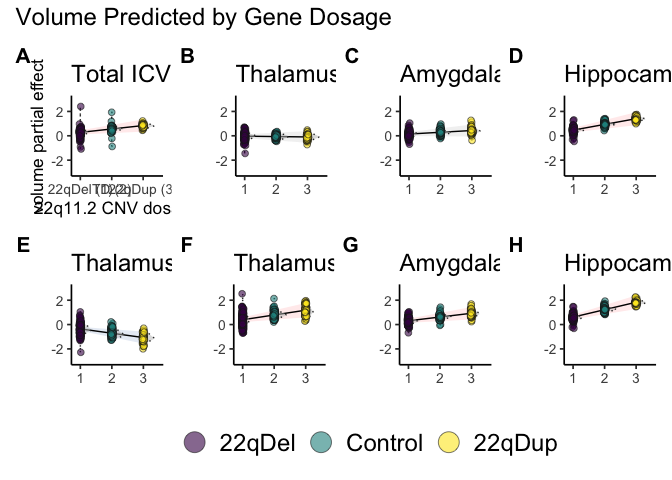
\includegraphics{22q_subcort_volumes_revised_files/figure-latex/unnamed-chunk-30-1.pdf}

\begin{Shaded}
\begin{Highlighting}[]
\CommentTok{\#ggsave(plot=lm\_fig\_all, filename=file.path(project,"figures/gene\_dosage/gene\_dosage\_all.pdf"), width=12, height=8.5, device = "pdf")}
\CommentTok{\#ggsave(plot=lm\_fig\_all, filename=file.path(project,"figures/gene\_dosage/gene\_dosage\_all.png"), width=12, height=8.5, device = "png", dpi = 300)}
\end{Highlighting}
\end{Shaded}

\hypertarget{age-curves-from-gamms}{%
\section{Age curves from GAMMs}\label{age-curves-from-gamms}}

wrap all maturational analyses in a function so that they can be
repeated with a truncated age subset of the input function allows for
exact replication of age analyses with multiple age ranges

\begin{Shaded}
\begin{Highlighting}[]
\CommentTok{\# the next few functions will be used inside of main\_maturation() }
\CommentTok{\# function to estimate smooths for plotting}
\NormalTok{smooth\_estimates\_se }\OtherTok{\textless{}{-}} \ControlFlowTok{function}\NormalTok{(gamm,smooth,n)\{}
\NormalTok{  out }\OtherTok{\textless{}{-}} \FunctionTok{smooth\_estimates}\NormalTok{(gamm,smooth,}\AttributeTok{n=}\NormalTok{n, }\AttributeTok{partial\_match =}\NormalTok{ T)}
\NormalTok{  out}\SpecialCharTok{$}\NormalTok{selo }\OtherTok{\textless{}{-}}\NormalTok{ out}\SpecialCharTok{$}\NormalTok{est }\SpecialCharTok{{-}}\NormalTok{ out}\SpecialCharTok{$}\NormalTok{se}
\NormalTok{  out}\SpecialCharTok{$}\NormalTok{sehi }\OtherTok{\textless{}{-}}\NormalTok{ out}\SpecialCharTok{$}\NormalTok{est }\SpecialCharTok{+}\NormalTok{ out}\SpecialCharTok{$}\NormalTok{se}
  \FunctionTok{return}\NormalTok{(out)}
\NormalTok{\}}

\CommentTok{\# function to take derivative output that includes an age smooth output age range where CI doesn\textquotesingle{}t include zero}
\CommentTok{\# adapted from https://github.com/pittnerdlab/22q11\_longitudinal\_cortical\_sMRI/blob/main/01a\_age\_effects.Rmd}
\NormalTok{get\_sig\_diff\_ages\_sc }\OtherTok{\textless{}{-}} \ControlFlowTok{function}\NormalTok{(gam, smooth, }\AttributeTok{group1=}\StringTok{"CONTROL"}\NormalTok{, group2)\{}
  \CommentTok{\# get derivative of specified smooth from gam}
\NormalTok{  diff }\OtherTok{\textless{}{-}} \FunctionTok{difference\_smooths}\NormalTok{(}\AttributeTok{model=}\NormalTok{gam, }\AttributeTok{smooth=}\NormalTok{smooth, }\AttributeTok{n=}\DecValTok{1000}\NormalTok{)}
  \CommentTok{\# filter for only chosen groups}
\NormalTok{  gdiff }\OtherTok{\textless{}{-}} \FunctionTok{filter}\NormalTok{(diff, level\_1}\SpecialCharTok{==}\NormalTok{group1 }\SpecialCharTok{\&}\NormalTok{ level\_2}\SpecialCharTok{==}\NormalTok{group2)}
  \CommentTok{\# get points where confidence interval doesn\textquotesingle{}t include zero}
\NormalTok{  sig }\OtherTok{\textless{}{-}} \FunctionTok{sign}\NormalTok{(gdiff}\SpecialCharTok{$}\NormalTok{lower) }\SpecialCharTok{==} \FunctionTok{sign}\NormalTok{(gdiff}\SpecialCharTok{$}\NormalTok{upper)}
  \CommentTok{\# get list of ages  }
\NormalTok{  agelist }\OtherTok{\textless{}{-}}\NormalTok{ gdiff}\SpecialCharTok{$}\NormalTok{AGE[sig]}
  \DocumentationTok{\#\# create age range from list of ages}
  \CommentTok{\# set age gap (years) between significant ages to be considered new range}
\NormalTok{  sigjump\_brain}\OtherTok{\textless{}{-}}\FloatTok{0.23}
\NormalTok{  j}\OtherTok{=}\DecValTok{1}
\NormalTok{  ranges}\OtherTok{=}\StringTok{""}
  \ControlFlowTok{if}\NormalTok{(}\FunctionTok{length}\NormalTok{(agelist)}\SpecialCharTok{\textgreater{}}\DecValTok{0}\NormalTok{) \{}
\NormalTok{    ranges}\OtherTok{\textless{}{-}}\FunctionTok{round}\NormalTok{(agelist[[j]],}\AttributeTok{digits=}\DecValTok{1}\NormalTok{)}
\NormalTok{  \}}
  \ControlFlowTok{while}\NormalTok{ (j }\SpecialCharTok{\textless{}} \FunctionTok{length}\NormalTok{(agelist)) \{}
\NormalTok{    j}\OtherTok{\textless{}{-}}\NormalTok{j}\SpecialCharTok{+}\DecValTok{1}
\NormalTok{    gdiff}\OtherTok{\textless{}{-}}\NormalTok{agelist[[j]]}\SpecialCharTok{{-}}\NormalTok{agelist[[j}\DecValTok{{-}1}\NormalTok{]]}
    \ControlFlowTok{if}\NormalTok{ (gdiff }\SpecialCharTok{\textgreater{}}\NormalTok{ sigjump\_brain) \{}
\NormalTok{      ranges}\OtherTok{\textless{}{-}}\FunctionTok{paste0}\NormalTok{(ranges,}\StringTok{"{-}"}\NormalTok{,}\FunctionTok{round}\NormalTok{(agelist[[j}\DecValTok{{-}1}\NormalTok{]],}\AttributeTok{digits=}\DecValTok{1}\NormalTok{),}\StringTok{"|"}\NormalTok{,}\FunctionTok{round}\NormalTok{(agelist[[j]],}\AttributeTok{digits=}\DecValTok{1}\NormalTok{))}
\NormalTok{    \}}
    \ControlFlowTok{if}\NormalTok{(j}\SpecialCharTok{==}\FunctionTok{length}\NormalTok{(agelist))\{}
\NormalTok{      ranges}\OtherTok{\textless{}{-}}\FunctionTok{paste0}\NormalTok{(ranges,}\StringTok{"{-}"}\NormalTok{,}\FunctionTok{round}\NormalTok{(agelist[[j]],}\AttributeTok{digits=}\DecValTok{1}\NormalTok{))}
\NormalTok{    \}}
\NormalTok{  \}}
  \FunctionTok{return}\NormalTok{(ranges)}
\NormalTok{\}}

\CommentTok{\# giant function to run all age curve analyses and output a set of stats and plots as a list object}
\NormalTok{main\_maturation }\OtherTok{\textless{}{-}} \ControlFlowTok{function}\NormalTok{(gam\_list)\{}
  \CommentTok{\# create empty list object to fill with results}
\NormalTok{  out }\OtherTok{\textless{}{-}} \FunctionTok{list}\NormalTok{()}
  
  \CommentTok{\# add initial gam list}
\NormalTok{  out}\SpecialCharTok{$}\NormalTok{gam\_list }\OtherTok{\textless{}{-}}\NormalTok{ gam\_list}
  
  \CommentTok{\# get smooth tables from gam}
\NormalTok{  stables }\OtherTok{\textless{}{-}} \FunctionTok{lapply}\NormalTok{(gam\_list,}\ControlFlowTok{function}\NormalTok{(g) }\FunctionTok{summary}\NormalTok{(g, }\AttributeTok{freq=}\NormalTok{T)}\SpecialCharTok{$}\NormalTok{s.table)}
  \CommentTok{\# retun smooth tables}
\NormalTok{  out}\SpecialCharTok{$}\NormalTok{stables }\OtherTok{\textless{}{-}}\NormalTok{ stables}
  
  \CommentTok{\# get p{-}vals}
\NormalTok{  del\_age\_pvals }\OtherTok{\textless{}{-}} \FunctionTok{lapply}\NormalTok{(stables, }\ControlFlowTok{function}\NormalTok{(s)s[}\StringTok{"s(AGE):SUBJECT\_IDENTITYPATIENT{-}DEL"}\NormalTok{,}\FunctionTok{c}\NormalTok{(}\StringTok{"F"}\NormalTok{,}\StringTok{"p{-}value"}\NormalTok{)]) }\SpecialCharTok{\%\textgreater{}\%} \FunctionTok{do.call}\NormalTok{(rbind,.) }\SpecialCharTok{\%\textgreater{}\%}\NormalTok{ data.frame }\SpecialCharTok{\%\textgreater{}\%} \FunctionTok{rename}\NormalTok{(}\StringTok{"age\_p\_val"}\OtherTok{=}\StringTok{"p.value"}\NormalTok{)}
\NormalTok{  del\_age\_pvals}\SpecialCharTok{$}\NormalTok{Region }\OtherTok{\textless{}{-}} \FunctionTok{rownames}\NormalTok{(del\_age\_pvals)}
\NormalTok{  del\_age\_pvals}\SpecialCharTok{$}\NormalTok{SUBJECT\_IDENTITY }\OtherTok{\textless{}{-}} \StringTok{"PATIENT{-}DEL"}
  
\NormalTok{  dup\_age\_pvals }\OtherTok{\textless{}{-}} \FunctionTok{lapply}\NormalTok{(stables, }\ControlFlowTok{function}\NormalTok{(s)s[}\StringTok{"s(AGE):SUBJECT\_IDENTITYPATIENT{-}DUP"}\NormalTok{,}\FunctionTok{c}\NormalTok{(}\StringTok{"F"}\NormalTok{,}\StringTok{"p{-}value"}\NormalTok{)]) }\SpecialCharTok{\%\textgreater{}\%} \FunctionTok{do.call}\NormalTok{(rbind,.) }\SpecialCharTok{\%\textgreater{}\%}\NormalTok{ data.frame }\SpecialCharTok{\%\textgreater{}\%} \FunctionTok{rename}\NormalTok{(}\StringTok{"age\_p\_val"}\OtherTok{=}\StringTok{"p.value"}\NormalTok{)}
\NormalTok{  dup\_age\_pvals}\SpecialCharTok{$}\NormalTok{Region }\OtherTok{\textless{}{-}} \FunctionTok{rownames}\NormalTok{(dup\_age\_pvals)}
\NormalTok{  dup\_age\_pvals}\SpecialCharTok{$}\NormalTok{SUBJECT\_IDENTITY }\OtherTok{\textless{}{-}} \StringTok{"PATIENT{-}DUP"}
  
\NormalTok{  hcs\_age\_pvals }\OtherTok{\textless{}{-}} \FunctionTok{lapply}\NormalTok{(stables, }\ControlFlowTok{function}\NormalTok{(s)s[}\StringTok{"s(AGE):SUBJECT\_IDENTITYCONTROL"}\NormalTok{,}\FunctionTok{c}\NormalTok{(}\StringTok{"F"}\NormalTok{,}\StringTok{"p{-}value"}\NormalTok{)]) }\SpecialCharTok{\%\textgreater{}\%} \FunctionTok{do.call}\NormalTok{(rbind,.) }\SpecialCharTok{\%\textgreater{}\%}\NormalTok{ data.frame  }\SpecialCharTok{\%\textgreater{}\%} \FunctionTok{rename}\NormalTok{(}\StringTok{"age\_p\_val"}\OtherTok{=}\StringTok{"p.value"}\NormalTok{)}
\NormalTok{  hcs\_age\_pvals}\SpecialCharTok{$}\NormalTok{Region }\OtherTok{\textless{}{-}} \FunctionTok{rownames}\NormalTok{(hcs\_age\_pvals)}
\NormalTok{  hcs\_age\_pvals}\SpecialCharTok{$}\NormalTok{SUBJECT\_IDENTITY }\OtherTok{\textless{}{-}} \StringTok{"CONTROL"}
  
  \CommentTok{\# correct for multiple comparisons (one test for age effects per group per network)}
\NormalTok{  all\_age\_pvals }\OtherTok{\textless{}{-}} \FunctionTok{rbind}\NormalTok{(del\_age\_pvals,dup\_age\_pvals,hcs\_age\_pvals)}
\NormalTok{  all\_age\_pvals}\SpecialCharTok{$}\NormalTok{age\_p\_val\_fdr }\OtherTok{\textless{}{-}}\NormalTok{ all\_age\_pvals}\SpecialCharTok{$}\NormalTok{age\_p\_val }\SpecialCharTok{\%\textgreater{}\%} \FunctionTok{p.adjust}\NormalTok{(., }\AttributeTok{method=}\StringTok{"fdr"}\NormalTok{)}
\NormalTok{  all\_age\_pvals}
  
  \CommentTok{\# make pretty table for export}
\NormalTok{  out\_age\_pvals }\OtherTok{\textless{}{-}}\NormalTok{ all\_age\_pvals[,}\FunctionTok{c}\NormalTok{(}\StringTok{"SUBJECT\_IDENTITY"}\NormalTok{,}\StringTok{"Region"}\NormalTok{,}\StringTok{"F"}\NormalTok{,}\StringTok{"age\_p\_val"}\NormalTok{,}\StringTok{"age\_p\_val\_fdr"}\NormalTok{)]}
  \FunctionTok{rownames}\NormalTok{(out\_age\_pvals) }\OtherTok{\textless{}{-}} \ConstantTok{NULL}
\NormalTok{  out\_age\_pvals }\OtherTok{\textless{}{-}} \FunctionTok{rename}\NormalTok{(out\_age\_pvals, }\StringTok{"p"}\OtherTok{=}\StringTok{"age\_p\_val"}\NormalTok{,}\StringTok{"FDR\_q"}\OtherTok{=}\StringTok{"age\_p\_val\_fdr"}\NormalTok{, }\StringTok{"Group"}\OtherTok{=}\StringTok{"SUBJECT\_IDENTITY"}\NormalTok{)}
\NormalTok{  out\_age\_pvals}\SpecialCharTok{$}\NormalTok{Group }\OtherTok{\textless{}{-}}\NormalTok{ out\_age\_pvals}\SpecialCharTok{$}\NormalTok{Group }\SpecialCharTok{\%\textgreater{}\%} \FunctionTok{gsub}\NormalTok{(}\StringTok{"CONTROL"}\NormalTok{,}\StringTok{"TD"}\NormalTok{,.) }\SpecialCharTok{\%\textgreater{}\%} \FunctionTok{gsub}\NormalTok{(}\StringTok{"PATIENT{-}DEL"}\NormalTok{,}\StringTok{"22qDel"}\NormalTok{,.) }\SpecialCharTok{\%\textgreater{}\%} \FunctionTok{gsub}\NormalTok{(}\StringTok{"PATIENT{-}DUP"}\NormalTok{,}\StringTok{"22qDup"}\NormalTok{,.)}
  \CommentTok{\#out\_age\_pvals$Region \textless{}{-} gsub(".combat","",out\_age\_pvals$Region)}
\NormalTok{  out\_age\_pvals}\SpecialCharTok{$}\NormalTok{Region }\OtherTok{\textless{}{-}} \FunctionTok{gsub}\NormalTok{(}\StringTok{".combat.norm"}\NormalTok{,}\StringTok{""}\NormalTok{,out\_age\_pvals}\SpecialCharTok{$}\NormalTok{Region)}
\NormalTok{  out\_age\_pvals}\SpecialCharTok{$}\NormalTok{F }\SpecialCharTok{\%\textless{}\textgreater{}\%} \FunctionTok{round}\NormalTok{(., }\AttributeTok{digits=}\DecValTok{2}\NormalTok{) }\SpecialCharTok{\%\textgreater{}\%} \FunctionTok{sprintf}\NormalTok{(}\StringTok{"\%.4f"}\NormalTok{,.)}
\NormalTok{  out\_age\_pvals}\SpecialCharTok{$}\NormalTok{p }\SpecialCharTok{\%\textless{}\textgreater{}\%} \FunctionTok{signif}\NormalTok{(., }\AttributeTok{digits=}\DecValTok{2}\NormalTok{) }\SpecialCharTok{\%\textgreater{}\%} \FunctionTok{sprintf}\NormalTok{(}\StringTok{"\%.3f"}\NormalTok{,.)}
\NormalTok{  out\_age\_pvals}\SpecialCharTok{$}\NormalTok{FDR\_q }\SpecialCharTok{\%\textless{}\textgreater{}\%} \FunctionTok{signif}\NormalTok{(., }\AttributeTok{digits=}\DecValTok{3}\NormalTok{) }\SpecialCharTok{\%\textgreater{}\%} \FunctionTok{sprintf}\NormalTok{(}\StringTok{"\%.4f"}\NormalTok{,.)}
  \CommentTok{\# retun age p{-}vals}
\NormalTok{  out}\SpecialCharTok{$}\NormalTok{out\_age\_pvals }\OtherTok{\textless{}{-}}\NormalTok{ out\_age\_pvals}
  
  \CommentTok{\# get only significant results}
\NormalTok{  out\_age\_pvals\_sig }\OtherTok{\textless{}{-}} \FunctionTok{filter}\NormalTok{(out\_age\_pvals, FDR\_q}\SpecialCharTok{\textless{}}\FloatTok{0.05}\NormalTok{)}
\NormalTok{  out\_age\_pvals\_sig}

  \CommentTok{\# get smooth estimate}
\NormalTok{  smooth\_all\_combat }\OtherTok{\textless{}{-}} \FunctionTok{lapply}\NormalTok{(gam\_list, }\ControlFlowTok{function}\NormalTok{(g) }\FunctionTok{smooth\_estimates\_se}\NormalTok{(}\AttributeTok{gamm=}\NormalTok{g, }\AttributeTok{smooth=}\StringTok{"s(AGE)"}\NormalTok{, }\AttributeTok{n=}\DecValTok{1000}\NormalTok{))}
  \CommentTok{\#names(smooth\_all\_combat) \textless{}{-} sc\_names\_combat}
  \FunctionTok{names}\NormalTok{(smooth\_all\_combat) }\OtherTok{\textless{}{-}}\NormalTok{ all\_names\_normed}
  \CommentTok{\# return smooth estimate}
\NormalTok{  out}\SpecialCharTok{$}\NormalTok{smooth\_all\_combat }\OtherTok{\textless{}{-}}\NormalTok{ smooth\_all\_combat}
  
  \CommentTok{\#get difference with TD smooth}
  \CommentTok{\# get all regions with a significant effect}
\NormalTok{  age\_regions }\OtherTok{\textless{}{-}}\NormalTok{ out\_age\_pvals\_sig}\SpecialCharTok{$}\NormalTok{Region }\SpecialCharTok{\%\textgreater{}\%}\NormalTok{ unique }\SpecialCharTok{\%\textgreater{}\%}\NormalTok{ sort}
\NormalTok{  age\_names }\OtherTok{\textless{}{-}} \FunctionTok{paste0}\NormalTok{(age\_regions,}\StringTok{".combat.norm"}\NormalTok{)}

  \CommentTok{\# get age ranges where del or dup significantly differ from td}
\NormalTok{  agediff\_td\_del }\OtherTok{\textless{}{-}} \FunctionTok{lapply}\NormalTok{(gam\_list[age\_names], }\ControlFlowTok{function}\NormalTok{(g) }\FunctionTok{get\_sig\_diff\_ages\_sc}\NormalTok{(}\AttributeTok{gam=}\NormalTok{g, }\AttributeTok{smooth=}\StringTok{"s(AGE)"}\NormalTok{,}\AttributeTok{group1=}\StringTok{"CONTROL"}\NormalTok{, }\AttributeTok{group2=}\StringTok{"PATIENT{-}DEL"}\NormalTok{))}
\NormalTok{  agediff\_td\_dup }\OtherTok{\textless{}{-}} \FunctionTok{lapply}\NormalTok{(gam\_list[age\_names], }\ControlFlowTok{function}\NormalTok{(g) }\FunctionTok{get\_sig\_diff\_ages\_sc}\NormalTok{(}\AttributeTok{gam=}\NormalTok{g, }\AttributeTok{smooth=}\StringTok{"s(AGE)"}\NormalTok{,}\AttributeTok{group1=}\StringTok{"CONTROL"}\NormalTok{, }\AttributeTok{group2=}\StringTok{"PATIENT{-}DUP"}\NormalTok{))}

  \CommentTok{\# organize age group differences by region and group}
\NormalTok{  age\_group\_diffs }\OtherTok{\textless{}{-}} \FunctionTok{data.frame}\NormalTok{(}\AttributeTok{FullName=}\FunctionTok{names}\NormalTok{(agediff\_td\_del), }\AttributeTok{td\_del=}\FunctionTok{as.vector}\NormalTok{(}\FunctionTok{unlist}\NormalTok{(agediff\_td\_del)),}\AttributeTok{td\_dup=}\FunctionTok{as.vector}\NormalTok{(}\FunctionTok{unlist}\NormalTok{(agediff\_td\_dup)))}
\NormalTok{  age\_group\_diffs}\SpecialCharTok{$}\NormalTok{Region }\OtherTok{\textless{}{-}} \FunctionTok{gsub}\NormalTok{(}\StringTok{".combat.norm"}\NormalTok{,}\StringTok{""}\NormalTok{, age\_group\_diffs}\SpecialCharTok{$}\NormalTok{FullName)}
  \CommentTok{\# return age group diffs}
\NormalTok{  out}\SpecialCharTok{$}\NormalTok{age\_group\_diffs }\OtherTok{\textless{}{-}}\NormalTok{ age\_group\_diffs}

  \CommentTok{\# convert to true/false for regions with or without a difference}
\NormalTok{  age\_group\_tf }\OtherTok{\textless{}{-}}\NormalTok{ (age\_group\_diffs }\SpecialCharTok{\%\textgreater{}\%}\NormalTok{ as.matrix }\SpecialCharTok{\%\textgreater{}\%}\NormalTok{ nchar) }\SpecialCharTok{!=}\DecValTok{0}
\NormalTok{  age\_group\_tf }\OtherTok{\textless{}{-}} \FunctionTok{data.frame}\NormalTok{(age\_group\_tf)}
\NormalTok{  age\_group\_tf}\SpecialCharTok{$}\NormalTok{Region }\OtherTok{\textless{}{-}}\NormalTok{ age\_group\_diffs}\SpecialCharTok{$}\NormalTok{Region}
\NormalTok{  age\_group\_tf}\SpecialCharTok{$}\NormalTok{either }\OtherTok{\textless{}{-}}\NormalTok{ age\_group\_tf}\SpecialCharTok{$}\NormalTok{td\_del }\SpecialCharTok{==} \ConstantTok{TRUE} \SpecialCharTok{|}\NormalTok{ age\_group\_tf}\SpecialCharTok{$}\NormalTok{td\_dup }\SpecialCharTok{==} \ConstantTok{TRUE}

  \CommentTok{\#make table of age differences for export}
\NormalTok{  age\_group\_export }\OtherTok{\textless{}{-}}\NormalTok{ age\_group\_diffs}
\NormalTok{  age\_group\_export}\SpecialCharTok{$}\NormalTok{bilat\_match }\OtherTok{\textless{}{-}}\NormalTok{ age\_group\_export}\SpecialCharTok{$}\NormalTok{Region }\SpecialCharTok{\%\textgreater{}\%} \FunctionTok{gsub}\NormalTok{(}\StringTok{"Thal\_"}\NormalTok{,}\StringTok{""}\NormalTok{,.) }\SpecialCharTok{\%\textgreater{}\%} \FunctionTok{gsub}\NormalTok{(}\StringTok{"Hip\_"}\NormalTok{,}\StringTok{""}\NormalTok{,.) }\SpecialCharTok{\%\textgreater{}\%} \FunctionTok{gsub}\NormalTok{(}\StringTok{"Amy\_"}\NormalTok{,}\StringTok{""}\NormalTok{,.)}
\NormalTok{  age\_group\_export  }\OtherTok{\textless{}{-}} \FunctionTok{merge}\NormalTok{(}\AttributeTok{x=}\NormalTok{age\_group\_export, }\AttributeTok{y=}\NormalTok{lut\_unique, }\AttributeTok{by=}\StringTok{"bilat\_match"}\NormalTok{)}

\NormalTok{  age\_group\_export\_final }\OtherTok{\textless{}{-}}\NormalTok{ age\_group\_export[,}\FunctionTok{c}\NormalTok{(}\StringTok{"Structure"}\NormalTok{,}\StringTok{"bilat\_name"}\NormalTok{,}\StringTok{"td\_del"}\NormalTok{,}\StringTok{"td\_dup"}\NormalTok{)]}
  \FunctionTok{colnames}\NormalTok{(age\_group\_export\_final) }\OtherTok{\textless{}{-}} \FunctionTok{c}\NormalTok{(}\StringTok{"Structure"}\NormalTok{,}\StringTok{"Region"}\NormalTok{,}\StringTok{"diff\_TD\_22qDel"}\NormalTok{,}\StringTok{"diff\_TD\_22qDup"}\NormalTok{)}
\NormalTok{  age\_group\_export\_final}\SpecialCharTok{$}\NormalTok{struct\_order }\OtherTok{\textless{}{-}}\NormalTok{ age\_group\_export\_final}\SpecialCharTok{$}\NormalTok{Structure }\SpecialCharTok{\%\textgreater{}\%} \FunctionTok{gsub}\NormalTok{(}\StringTok{"whole brain"}\NormalTok{,}\DecValTok{1}\NormalTok{,.) }\SpecialCharTok{\%\textgreater{}\%} \FunctionTok{gsub}\NormalTok{(}\StringTok{"thalamus"}\NormalTok{,}\DecValTok{2}\NormalTok{,.) }\SpecialCharTok{\%\textgreater{}\%} \FunctionTok{gsub}\NormalTok{(}\StringTok{"hippocampus"}\NormalTok{,}\DecValTok{3}\NormalTok{,.) }\SpecialCharTok{\%\textgreater{}\%} \FunctionTok{gsub}\NormalTok{(}\StringTok{"amygdala"}\NormalTok{,}\DecValTok{4}\NormalTok{,.)}
\NormalTok{  age\_group\_export\_final }\OtherTok{\textless{}{-}}\NormalTok{ age\_group\_export\_final[}\FunctionTok{with}\NormalTok{(age\_group\_export\_final, }\FunctionTok{order}\NormalTok{(struct\_order,Region)),]}
\NormalTok{  age\_group\_export\_final }\OtherTok{\textless{}{-}} \FunctionTok{subset}\NormalTok{(age\_group\_export\_final, }\AttributeTok{select=}\SpecialCharTok{{-}}\NormalTok{struct\_order)}

  \CommentTok{\# edit structure names}
\NormalTok{  structure\_dup }\OtherTok{\textless{}{-}} \FunctionTok{duplicated}\NormalTok{(age\_group\_export\_final}\SpecialCharTok{$}\NormalTok{Structure)}
  \ControlFlowTok{for}\NormalTok{(i }\ControlFlowTok{in} \DecValTok{1}\SpecialCharTok{:}\FunctionTok{length}\NormalTok{(structure\_dup))\{}
    \ControlFlowTok{if}\NormalTok{(structure\_dup[i]}\SpecialCharTok{==}\ConstantTok{TRUE}\NormalTok{)\{}
\NormalTok{      age\_group\_export\_final[i,}\StringTok{"Structure"}\NormalTok{] }\OtherTok{\textless{}{-}} \StringTok{""}
\NormalTok{    \}}
\NormalTok{  \}}

  \CommentTok{\# return age group final table}
\NormalTok{  out}\SpecialCharTok{$}\NormalTok{age\_group\_export\_final }\OtherTok{\textless{}{-}}\NormalTok{ age\_group\_export\_final}
  \CommentTok{\#write.csv(age\_group\_export\_final[,c("Structure","Region","diff\_TD\_22qDel","diff\_TD\_22qDup")], file=file.path(project,"figures/age/age\_differences.csv"), row.names = FALSE)}

  \CommentTok{\#plot summary of GAMM results}
  \CommentTok{\# split data frames by group}
\NormalTok{  sig\_del }\OtherTok{\textless{}{-}} \FunctionTok{filter}\NormalTok{(out\_age\_pvals\_sig, Group}\SpecialCharTok{==}\StringTok{"22qDel"}\NormalTok{)}
\NormalTok{  sig\_dup }\OtherTok{\textless{}{-}} \FunctionTok{filter}\NormalTok{(out\_age\_pvals\_sig, Group}\SpecialCharTok{==}\StringTok{"22qDup"}\NormalTok{)}
\NormalTok{  sig\_hcs }\OtherTok{\textless{}{-}} \FunctionTok{filter}\NormalTok{(out\_age\_pvals\_sig, Group}\SpecialCharTok{==}\StringTok{"TD"}\NormalTok{)}

  \CommentTok{\# list of unique regions with significance in 22q or TD}
\NormalTok{  sig\_regions\_compare }\OtherTok{\textless{}{-}} \FunctionTok{data.frame}\NormalTok{(}\AttributeTok{Region=}\FunctionTok{sort}\NormalTok{(}\FunctionTok{unique}\NormalTok{(out\_age\_pvals\_sig}\SpecialCharTok{$}\NormalTok{Region)))}
  \FunctionTok{row.names}\NormalTok{(sig\_regions\_compare) }\OtherTok{\textless{}{-}}\NormalTok{ sig\_regions\_compare}\SpecialCharTok{$}\NormalTok{Region}

  \ControlFlowTok{for}\NormalTok{ (region }\ControlFlowTok{in}\NormalTok{ sig\_regions\_compare}\SpecialCharTok{$}\NormalTok{Region)\{}
\NormalTok{    sig\_regions\_compare[region,}\StringTok{"22qDel"}\NormalTok{] }\OtherTok{\textless{}{-}}\NormalTok{ region }\SpecialCharTok{\%in\%}\NormalTok{ sig\_del}\SpecialCharTok{$}\NormalTok{Region}
    \CommentTok{\#sig\_regions\_compare[region,"Del\_u30"] \textless{}{-} region \%in\% sig\_del\_u30$Region}
\NormalTok{    sig\_regions\_compare[region,}\StringTok{"22qDup"}\NormalTok{] }\OtherTok{\textless{}{-}}\NormalTok{ region }\SpecialCharTok{\%in\%}\NormalTok{ sig\_dup}\SpecialCharTok{$}\NormalTok{Region}
    \CommentTok{\#sig\_regions\_compare[region,"Dup\_u30"] \textless{}{-} region \%in\% sig\_dup\_u30$Region}
\NormalTok{    sig\_regions\_compare[region,}\StringTok{"TD"}\NormalTok{]}\OtherTok{\textless{}{-}}\NormalTok{ region }\SpecialCharTok{\%in\%}\NormalTok{ sig\_hcs}\SpecialCharTok{$}\NormalTok{Region}
    \CommentTok{\#sig\_regions\_compare[region,"TD\_u30"] \textless{}{-} region \%in\% sig\_hcs\_u30$Region}
\NormalTok{  \}}
  \CommentTok{\#sig\_regions\_compare}

  \CommentTok{\# create new column with TRUE if not also significant in TD}
\NormalTok{  sig\_regions\_compare}\SpecialCharTok{$}\NormalTok{TD\_sig }\OtherTok{\textless{}{-}} \ConstantTok{NA}
  \ControlFlowTok{for}\NormalTok{ (r }\ControlFlowTok{in} \DecValTok{1}\SpecialCharTok{:}\FunctionTok{nrow}\NormalTok{(sig\_regions\_compare))\{}
\NormalTok{    td }\OtherTok{\textless{}{-}}\NormalTok{ sig\_regions\_compare[r,}\StringTok{"TD"}\NormalTok{]}
    \CommentTok{\#td30 \textless{}{-} sig\_regions\_compare[r,"TD\_u30"]}
    \ControlFlowTok{if}\NormalTok{ (td}\SpecialCharTok{==}\ConstantTok{TRUE}\NormalTok{)\{}
\NormalTok{      sig\_regions\_compare[r,}\StringTok{"TD\_sig"}\NormalTok{] }\OtherTok{\textless{}{-}} \ConstantTok{TRUE}
\NormalTok{    \}}\ControlFlowTok{else}\NormalTok{\{}
\NormalTok{      sig\_regions\_compare[r,}\StringTok{"TD\_sig"}\NormalTok{] }\OtherTok{\textless{}{-}} \ConstantTok{FALSE}
\NormalTok{    \}}
\NormalTok{  \}}

  \CommentTok{\# return comparison of regions}
\NormalTok{  out}\SpecialCharTok{$}\NormalTok{sig\_regions\_compare }\OtherTok{\textless{}{-}}\NormalTok{ sig\_regions\_compare}

  \CommentTok{\# create long df for plotting}
  \FunctionTok{setDT}\NormalTok{(sig\_regions\_compare)}
\NormalTok{  idvars}\OtherTok{=}\FunctionTok{c}\NormalTok{(}\StringTok{"Region"}\NormalTok{,}\StringTok{"TD\_sig"}\NormalTok{)}
\NormalTok{  compare\_long }\OtherTok{\textless{}{-}} \FunctionTok{melt.data.table}\NormalTok{(sig\_regions\_compare, }\AttributeTok{id.vars =}\NormalTok{ idvars, }\AttributeTok{measure.vars =} \FunctionTok{names}\NormalTok{(sig\_regions\_compare)[}\FunctionTok{which}\NormalTok{(}\SpecialCharTok{!}\FunctionTok{names}\NormalTok{(sig\_regions\_compare) }\SpecialCharTok{\%in\%}\NormalTok{ idvars)])}
\NormalTok{  compare\_long}\SpecialCharTok{$}\NormalTok{Region }\SpecialCharTok{\%\textless{}\textgreater{}\%}\NormalTok{ as.factor}

  \CommentTok{\# order by region, then group}
  \FunctionTok{setorder}\NormalTok{(compare\_long, Region, variable)}

  \CommentTok{\# for plotting, create new column with TRUE if the value at row r is equal to row r{-}1 (excluding rows where variable is del\_all)}
\NormalTok{  compare\_long}\SpecialCharTok{$}\NormalTok{postmatch }\OtherTok{\textless{}{-}} \ConstantTok{NA}
  \ControlFlowTok{for}\NormalTok{ (r }\ControlFlowTok{in} \DecValTok{1}\SpecialCharTok{:}\NormalTok{(}\FunctionTok{nrow}\NormalTok{(compare\_long)}\SpecialCharTok{{-}}\DecValTok{1}\NormalTok{))\{}
\NormalTok{    val }\OtherTok{\textless{}{-}}\NormalTok{ compare\_long[r,}\StringTok{"value"}\NormalTok{]}
\NormalTok{    postval }\OtherTok{\textless{}{-}}\NormalTok{ compare\_long[(r}\SpecialCharTok{+}\DecValTok{1}\NormalTok{),}\StringTok{"value"}\NormalTok{]}
    \ControlFlowTok{if}\NormalTok{ (val}\SpecialCharTok{==}\ConstantTok{TRUE} \SpecialCharTok{\&}\NormalTok{ postval}\SpecialCharTok{==}\ConstantTok{TRUE}\NormalTok{)\{}
\NormalTok{      compare\_long[r,}\StringTok{"postmatch"}\NormalTok{] }\OtherTok{\textless{}{-}} \ConstantTok{TRUE}
\NormalTok{    \}}\ControlFlowTok{else}\NormalTok{\{}
\NormalTok{      compare\_long[r,}\StringTok{"postmatch"}\NormalTok{] }\OtherTok{\textless{}{-}} \ConstantTok{FALSE}
\NormalTok{    \}}
\NormalTok{  \}}
  \CommentTok{\# set to NA group that will be rightmost column of plot}
\NormalTok{  groups }\OtherTok{\textless{}{-}} \FunctionTok{levels}\NormalTok{(compare\_long}\SpecialCharTok{$}\NormalTok{variable)}
\NormalTok{  last\_group }\OtherTok{\textless{}{-}}\NormalTok{ groups[}\FunctionTok{length}\NormalTok{(groups)]}
\NormalTok{  compare\_long[}\FunctionTok{which}\NormalTok{(compare\_long}\SpecialCharTok{$}\NormalTok{variable}\SpecialCharTok{==}\NormalTok{last\_group),}\StringTok{"postmatch"}\NormalTok{] }\OtherTok{\textless{}{-}} \ConstantTok{NA}

  \CommentTok{\# create column with TRUE if pt group is significant but TD are not}
\NormalTok{  compare\_long}\SpecialCharTok{$}\NormalTok{pt\_sig\_only }\OtherTok{\textless{}{-}} \ConstantTok{NA}
  \ControlFlowTok{for}\NormalTok{ (r }\ControlFlowTok{in} \DecValTok{1}\SpecialCharTok{:}\NormalTok{(}\FunctionTok{nrow}\NormalTok{(compare\_long)))\{}
    \ControlFlowTok{if}\NormalTok{(compare\_long[r,}\StringTok{"TD\_sig"}\NormalTok{]}\SpecialCharTok{==}\ConstantTok{FALSE} \SpecialCharTok{\&}\NormalTok{ compare\_long[r,}\StringTok{"value"}\NormalTok{]}\SpecialCharTok{==}\ConstantTok{TRUE}\NormalTok{)\{}
      \CommentTok{\#if(compare\_long[r,"TD"]==FALSE \& compare\_long[r,"value"]==TRUE)\{}
\NormalTok{      compare\_long[r,}\StringTok{"pt\_sig\_only"}\NormalTok{] }\OtherTok{\textless{}{-}} \ConstantTok{TRUE}
\NormalTok{    \}}
    \CommentTok{\#if(compare\_long[r,"variable"]=="TD\_all" | compare\_long[r,"variable"]=="TD\_u30")\{}
    \ControlFlowTok{if}\NormalTok{(compare\_long[r,}\StringTok{"variable"}\NormalTok{]}\SpecialCharTok{==}\StringTok{"TD\_all"}\NormalTok{)\{}
\NormalTok{      compare\_long[r,}\StringTok{"pt\_sig\_only"}\NormalTok{] }\OtherTok{\textless{}{-}} \ConstantTok{NA}
\NormalTok{    \}}
\NormalTok{  \}}
  \CommentTok{\# replace NA with FALSE}
\NormalTok{  compare\_long }\OtherTok{\textless{}{-}} \FunctionTok{replace\_na}\NormalTok{(compare\_long, }\FunctionTok{list}\NormalTok{(}\AttributeTok{pt\_sig\_only=}\ConstantTok{FALSE}\NormalTok{))}
  
  \CommentTok{\# edit region names to remove trailing underscore and "\_all", replace other underscores with space, and capitalize first letter without editing subsequent letters}
  \CommentTok{\#compare\_long$Region\_edit \textless{}{-} compare\_long$Region \%\textgreater{}\% gsub("\_$","",.) \%\textgreater{}\% gsub("\_all","",.) \%\textgreater{}\% gsub("\_"," ",.) \%\textgreater{}\% gsub("\textbackslash{}\textbackslash{}b([a{-}z])", "\textbackslash{}\textbackslash{}U\textbackslash{}\textbackslash{}1",., perl=TRUE)}
\NormalTok{  compare\_long}\SpecialCharTok{$}\NormalTok{bilat\_match }\OtherTok{\textless{}{-}}\NormalTok{ compare\_long}\SpecialCharTok{$}\NormalTok{Region }\SpecialCharTok{\%\textgreater{}\%} \FunctionTok{gsub}\NormalTok{(}\StringTok{"Thal\_"}\NormalTok{,}\StringTok{""}\NormalTok{,.) }\SpecialCharTok{\%\textgreater{}\%} \FunctionTok{gsub}\NormalTok{(}\StringTok{"Hip\_"}\NormalTok{,}\StringTok{""}\NormalTok{,.) }\SpecialCharTok{\%\textgreater{}\%} \FunctionTok{gsub}\NormalTok{(}\StringTok{"Amy\_"}\NormalTok{,}\StringTok{""}\NormalTok{,.)}
\NormalTok{  compare\_long }\OtherTok{\textless{}{-}} \FunctionTok{merge}\NormalTok{(}\AttributeTok{x=}\NormalTok{compare\_long, }\AttributeTok{y=}\NormalTok{lut\_unique[,}\FunctionTok{c}\NormalTok{(}\StringTok{"bilat\_name"}\NormalTok{,}\StringTok{"bilat\_match"}\NormalTok{,}\StringTok{"Structure"}\NormalTok{)], }\AttributeTok{by=}\StringTok{"bilat\_match"}\NormalTok{, }\AttributeTok{all.x=}\ConstantTok{TRUE}\NormalTok{)}
  \CommentTok{\#compare\_long$Region\_edit \textless{}{-} paste(compare\_long$Structure, compare\_long$bilat\_name)}
\NormalTok{  compare\_long}\SpecialCharTok{$}\NormalTok{Region\_edit1 }\OtherTok{\textless{}{-}}\NormalTok{ compare\_long}\SpecialCharTok{$}\NormalTok{bilat\_name }\SpecialCharTok{\%\textgreater{}\%} \FunctionTok{gsub}\NormalTok{(}\StringTok{"hippocampal amygdala transition area"}\NormalTok{,}\StringTok{"HATA"}\NormalTok{,.) }\SpecialCharTok{\%\textgreater{}\%} \FunctionTok{gsub}\NormalTok{(}\StringTok{"hippocampus"}\NormalTok{,}\StringTok{""}\NormalTok{,.) }\SpecialCharTok{\%\textgreater{}\%} \FunctionTok{gsub}\NormalTok{(}\StringTok{"thalamus"}\NormalTok{,}\StringTok{""}\NormalTok{,.) }\SpecialCharTok{\%\textgreater{}\%}   \FunctionTok{gsub}\NormalTok{(}\StringTok{"amygdala"}\NormalTok{,}\StringTok{""}\NormalTok{,.) }\SpecialCharTok{\%\textgreater{}\%} \FunctionTok{gsub}\NormalTok{(}\StringTok{" $"}\NormalTok{,}\StringTok{""}\NormalTok{,.) }\SpecialCharTok{\%\textgreater{}\%} \FunctionTok{gsub}\NormalTok{(}\StringTok{"  "}\NormalTok{,}\StringTok{" "}\NormalTok{,.)}

\NormalTok{  region\_edit\_df }\OtherTok{\textless{}{-}} \FunctionTok{data.frame}\NormalTok{(}\AttributeTok{col1=}\NormalTok{compare\_long}\SpecialCharTok{$}\NormalTok{Region\_edit1, }\AttributeTok{col2=}\NormalTok{compare\_long}\SpecialCharTok{$}\NormalTok{Structure)}
\NormalTok{  region\_edit\_df }\OtherTok{\textless{}{-}}\NormalTok{ region\_edit\_df[}\SpecialCharTok{!}\FunctionTok{duplicated}\NormalTok{(region\_edit\_df),]}
  \FunctionTok{setorder}\NormalTok{(region\_edit\_df, col2, col1)}
\NormalTok{  region\_levels}\OtherTok{\textless{}{-}} \FunctionTok{paste}\NormalTok{(region\_edit\_df}\SpecialCharTok{$}\NormalTok{col1, region\_edit\_df}\SpecialCharTok{$}\NormalTok{col2)}

\NormalTok{  compare\_long}\SpecialCharTok{$}\NormalTok{Region\_edit }\OtherTok{\textless{}{-}} \FunctionTok{factor}\NormalTok{(}\AttributeTok{x=}\FunctionTok{paste}\NormalTok{(compare\_long}\SpecialCharTok{$}\NormalTok{Region\_edit1, compare\_long}\SpecialCharTok{$}\NormalTok{Structure), }\AttributeTok{levels=}\NormalTok{region\_levels)}
  \CommentTok{\#compare\_long$Region\_edit \textless{}{-} paste(compare\_long$Structure, compare\_long$Region\_edit1)}
  \CommentTok{\#compare\_long$Region\_edit \textless{}{-} compare\_long$Region\_edit \%\textgreater{}\% gsub("hippocampal  transition area hippocampus", "HATA hippocampus",.) \%\textgreater{}\% gsub("  "," ",.)}

  \CommentTok{\# add column with true if there is a group difference between patients and controls}
  \CommentTok{\#compare\_long \textless{}{-} merge(x=compare\_long, y=age\_group\_tf[,c("Region","either")], by="Region")}
\NormalTok{  compare\_long}\SpecialCharTok{$}\NormalTok{gdiff }\OtherTok{\textless{}{-}} \ConstantTok{NA}
  \ControlFlowTok{for}\NormalTok{ (i }\ControlFlowTok{in} \DecValTok{1}\SpecialCharTok{:}\FunctionTok{nrow}\NormalTok{(compare\_long))\{}
    \CommentTok{\#print(i)}
\NormalTok{    region }\OtherTok{\textless{}{-}}\NormalTok{ compare\_long[i,}\StringTok{"Region"}\NormalTok{] }\SpecialCharTok{\%\textgreater{}\%}\NormalTok{ as.matrix }\SpecialCharTok{\%\textgreater{}\%}\NormalTok{ as.character}
    \CommentTok{\#print(region)}
\NormalTok{    variable }\OtherTok{\textless{}{-}}\NormalTok{ compare\_long[i,}\StringTok{"variable"}\NormalTok{] }\SpecialCharTok{\%\textgreater{}\%}\NormalTok{ as.matrix }\SpecialCharTok{\%\textgreater{}\%}\NormalTok{ as.character}
    \CommentTok{\#print(variable)}
\NormalTok{    gdiff }\OtherTok{\textless{}{-}} \ConstantTok{NA}
    \ControlFlowTok{if}\NormalTok{(variable}\SpecialCharTok{==}\StringTok{"22qDel"}\NormalTok{)\{}
\NormalTok{      gdiff }\OtherTok{\textless{}{-}} \FunctionTok{filter}\NormalTok{(age\_group\_tf, Region}\SpecialCharTok{==}\NormalTok{region)}\SpecialCharTok{$}\NormalTok{td\_del}
\NormalTok{    \}}\ControlFlowTok{else} \ControlFlowTok{if}\NormalTok{(variable}\SpecialCharTok{==}\StringTok{"22qDup"}\NormalTok{)\{}
\NormalTok{      gdiff }\OtherTok{\textless{}{-}} \FunctionTok{filter}\NormalTok{(age\_group\_tf, Region}\SpecialCharTok{==}\NormalTok{region)}\SpecialCharTok{$}\NormalTok{td\_dup}
\NormalTok{    \}}\ControlFlowTok{else} \ControlFlowTok{if}\NormalTok{(variable}\SpecialCharTok{==}\StringTok{"TD"}\NormalTok{)\{}
\NormalTok{      gdiff }\OtherTok{\textless{}{-}} \FunctionTok{filter}\NormalTok{(age\_group\_tf, Region}\SpecialCharTok{==}\NormalTok{region)}\SpecialCharTok{$}\NormalTok{either}
\NormalTok{    \}}
    \CommentTok{\#print(gdiff)}
\NormalTok{    compare\_long[i,}\StringTok{"gdiff"}\NormalTok{] }\OtherTok{\textless{}{-}}\NormalTok{ gdiff}
\NormalTok{  \}}

  \CommentTok{\# return compare\_long }
\NormalTok{  out}\SpecialCharTok{$}\NormalTok{compare\_long }\OtherTok{\textless{}{-}}\NormalTok{ compare\_long}

  \CommentTok{\# plot}
\NormalTok{  gamm\_compare }\OtherTok{\textless{}{-}} \FunctionTok{ggplot}\NormalTok{(}\AttributeTok{data=}\NormalTok{compare\_long, }\FunctionTok{aes}\NormalTok{(}\AttributeTok{y=}\NormalTok{Region\_edit, }\AttributeTok{x=}\NormalTok{variable))}\SpecialCharTok{+}
    \FunctionTok{geom\_line}\NormalTok{(}\FunctionTok{aes}\NormalTok{(}\AttributeTok{group=}\NormalTok{Region, }\AttributeTok{color=}\NormalTok{postmatch),}\AttributeTok{alpha=}\FloatTok{0.4}\NormalTok{, }\AttributeTok{show.legend =} \ConstantTok{FALSE}\NormalTok{)}\SpecialCharTok{+}
    \FunctionTok{scale\_color\_manual}\NormalTok{(}\AttributeTok{values=}\FunctionTok{c}\NormalTok{(}\StringTok{"white"}\NormalTok{, }\StringTok{"black"}\NormalTok{))}\SpecialCharTok{+}
    \FunctionTok{new\_scale\_color}\NormalTok{()}\SpecialCharTok{+}
    \FunctionTok{geom\_point}\NormalTok{(}\FunctionTok{aes}\NormalTok{(}\AttributeTok{shape=}\NormalTok{value, }\AttributeTok{size=}\NormalTok{gdiff, }\AttributeTok{color=}\NormalTok{pt\_sig\_only, }\AttributeTok{alpha=}\NormalTok{value))}\SpecialCharTok{+}
    \FunctionTok{scale\_shape\_manual}\NormalTok{(}\AttributeTok{values=}\FunctionTok{c}\NormalTok{(}\DecValTok{1}\NormalTok{,}\DecValTok{16}\NormalTok{))}\SpecialCharTok{+}
    \FunctionTok{scale\_alpha\_manual}\NormalTok{(}\AttributeTok{values=}\FunctionTok{c}\NormalTok{(}\FloatTok{0.3}\NormalTok{,}\DecValTok{1}\NormalTok{))}\SpecialCharTok{+}
    \FunctionTok{scale\_size\_manual}\NormalTok{(}\AttributeTok{values=}\FunctionTok{c}\NormalTok{(}\DecValTok{2}\NormalTok{,}\DecValTok{4}\NormalTok{))}\SpecialCharTok{+}
    \FunctionTok{scale\_color\_manual}\NormalTok{(}\AttributeTok{values =} \FunctionTok{c}\NormalTok{(}\StringTok{"black"}\NormalTok{,}\StringTok{"red"}\NormalTok{), }\AttributeTok{na.value =} \StringTok{"black"}\NormalTok{)}\SpecialCharTok{+}
    \FunctionTok{labs}\NormalTok{(}\AttributeTok{shape=}\StringTok{"Age: FDR q \textless{} 0.05"}\NormalTok{, }\AttributeTok{alpha=}\StringTok{"Age: FDR q \textless{} 0.05"}\NormalTok{,}\AttributeTok{size=}\StringTok{"Group Difference"}\NormalTok{, }\AttributeTok{color=}\StringTok{"Significant in}\SpecialCharTok{\textbackslash{}n}\StringTok{Patients only"}\NormalTok{)}\SpecialCharTok{+}
    \FunctionTok{guides}\NormalTok{(}\AttributeTok{alpha =} \FunctionTok{guide\_legend}\NormalTok{(}\AttributeTok{order =} \DecValTok{1}\NormalTok{),}
           \AttributeTok{shape =} \FunctionTok{guide\_legend}\NormalTok{(}\AttributeTok{order =} \DecValTok{1}\NormalTok{, }\AttributeTok{override.aes=}\FunctionTok{list}\NormalTok{(}\AttributeTok{size=}\DecValTok{2}\NormalTok{)),}
           \CommentTok{\#shape = guide\_legend(order = 1, override.aes=list(size=4, shape=c(0,15))),}
           \AttributeTok{size  =} \FunctionTok{guide\_legend}\NormalTok{(}\AttributeTok{order =} \DecValTok{2}\NormalTok{),}
           \CommentTok{\#color  = guide\_legend(order = 3, override.aes=list(size=4, shape=15)))+}
           \AttributeTok{color  =} \FunctionTok{guide\_legend}\NormalTok{(}\AttributeTok{order =} \DecValTok{3}\NormalTok{, }\AttributeTok{override.aes=}\FunctionTok{list}\NormalTok{(}\AttributeTok{size=}\DecValTok{2}\NormalTok{)))}\SpecialCharTok{+}
    \FunctionTok{scale\_x\_discrete}\NormalTok{(}\AttributeTok{position =} \StringTok{"top"}\NormalTok{)}\SpecialCharTok{+}
    \FunctionTok{xlab}\NormalTok{(}\ConstantTok{NULL}\NormalTok{)}\SpecialCharTok{+}
    \FunctionTok{ylab}\NormalTok{(}\StringTok{"Region"}\NormalTok{)}\SpecialCharTok{+}
    \FunctionTok{ggtitle}\NormalTok{(}\StringTok{"Significant Age Effects by Cohort"}\NormalTok{)}\SpecialCharTok{+}
    \FunctionTok{theme\_bw}\NormalTok{(}\AttributeTok{base\_size =} \DecValTok{12}\NormalTok{)}\SpecialCharTok{+}
    \FunctionTok{theme}\NormalTok{(}\AttributeTok{panel.grid.major =} \FunctionTok{element\_blank}\NormalTok{(),}\AttributeTok{panel.grid.minor =} \FunctionTok{element\_blank}\NormalTok{(), }\AttributeTok{axis.ticks.x=}\FunctionTok{element\_blank}\NormalTok{())}

  \CommentTok{\#gamm\_compare}
  \CommentTok{\# return gamm comparison plot}
\NormalTok{  out}\SpecialCharTok{$}\NormalTok{gamm\_compare }\OtherTok{\textless{}{-}}\NormalTok{ gamm\_compare}
  \CommentTok{\#ggsave(plot=gamm\_compare, filename=file.path(project,"figures/age/age\_gamm\_group\_compare.pdf"), width=7, height=5, device = "pdf")}
  \CommentTok{\#ggsave(plot=gamm\_compare, filename=file.path(project,"figures/age/age\_gamm\_group\_compare.png"), width=7, height=5, device = "png", dpi = 300)}

  \CommentTok{\#return final list object}
  \FunctionTok{return}\NormalTok{(out)}
\NormalTok{\}}
\end{Highlighting}
\end{Shaded}

do maturation analyses

\begin{Shaded}
\begin{Highlighting}[]
\CommentTok{\# full age range}
\NormalTok{maturation\_full }\OtherTok{\textless{}{-}} \FunctionTok{main\_maturation}\NormalTok{(}\AttributeTok{gam\_list=}\NormalTok{gamm\_combat)}
\CommentTok{\# removing oldest participants (over 35 years)}
\NormalTok{maturation\_young }\OtherTok{\textless{}{-}} \FunctionTok{main\_maturation}\NormalTok{(}\AttributeTok{gam\_list=}\NormalTok{gamm\_combat\_young)}
\end{Highlighting}
\end{Shaded}

in smooth tables, mark age ranges of significant difference to controls

\begin{Shaded}
\begin{Highlighting}[]
\CommentTok{\# function to add true/false for significant difference to TD group to smooth tables}
\NormalTok{gdiff\_smooth }\OtherTok{\textless{}{-}} \ControlFlowTok{function}\NormalTok{(mature)\{}
  \CommentTok{\# make new list of smooths to edit}
\NormalTok{  mature}\SpecialCharTok{$}\NormalTok{smooth\_all\_gdiff }\OtherTok{\textless{}{-}}\NormalTok{ mature}\SpecialCharTok{$}\NormalTok{smooth\_all\_combat}
  \CommentTok{\# create a column to mark group difference from TD, and first set all to FALSE}
  \ControlFlowTok{for}\NormalTok{(i }\ControlFlowTok{in} \DecValTok{1}\SpecialCharTok{:}\FunctionTok{length}\NormalTok{(mature}\SpecialCharTok{$}\NormalTok{smooth\_all\_gdiff))\{}
\NormalTok{    mature}\SpecialCharTok{$}\NormalTok{smooth\_all\_gdiff[[i]]}\SpecialCharTok{$}\NormalTok{gdiff }\OtherTok{\textless{}{-}} \ConstantTok{FALSE}
\NormalTok{  \}}
  \CommentTok{\# list of regions with some group diff}
\NormalTok{  regions }\OtherTok{\textless{}{-}}\NormalTok{ mature}\SpecialCharTok{$}\NormalTok{age\_group\_diffs}\SpecialCharTok{$}\NormalTok{FullName}
  \CommentTok{\# update smooth\_all\_gdiff}
  \ControlFlowTok{for}\NormalTok{(r }\ControlFlowTok{in} \DecValTok{1}\SpecialCharTok{:}\FunctionTok{length}\NormalTok{(regions))\{}
\NormalTok{    name }\OtherTok{\textless{}{-}}\NormalTok{ mature}\SpecialCharTok{$}\NormalTok{age\_group\_diffs[r,}\StringTok{"FullName"}\NormalTok{]}
\NormalTok{    td\_del }\OtherTok{\textless{}{-}}\NormalTok{ mature}\SpecialCharTok{$}\NormalTok{age\_group\_diffs[r,}\StringTok{"td\_del"}\NormalTok{]}
\NormalTok{    td\_dup }\OtherTok{\textless{}{-}}\NormalTok{ mature}\SpecialCharTok{$}\NormalTok{age\_group\_diffs[r,}\StringTok{"td\_dup"}\NormalTok{]}
    \CommentTok{\# get periods of significant difference}
    \ControlFlowTok{if}\NormalTok{(}\FunctionTok{nchar}\NormalTok{(td\_del)}\SpecialCharTok{\textgreater{}}\DecValTok{1}\NormalTok{)\{}
      \CommentTok{\# split individual periods}
\NormalTok{      periods }\OtherTok{\textless{}{-}} \FunctionTok{str\_split}\NormalTok{(}\AttributeTok{string=}\NormalTok{td\_del, }\AttributeTok{pattern=}\StringTok{"}\SpecialCharTok{\textbackslash{}\textbackslash{}}\StringTok{|"}\NormalTok{)[[}\DecValTok{1}\NormalTok{]]}
      \ControlFlowTok{for}\NormalTok{(t }\ControlFlowTok{in} \DecValTok{1}\SpecialCharTok{:}\FunctionTok{length}\NormalTok{(periods))\{}
        \CommentTok{\# get start and stop age}
\NormalTok{        ages }\OtherTok{\textless{}{-}} \FunctionTok{str\_split}\NormalTok{(}\AttributeTok{string=}\NormalTok{periods[t], }\AttributeTok{pattern=}\StringTok{"{-}"}\NormalTok{)[[}\DecValTok{1}\NormalTok{]]}
\NormalTok{        start }\OtherTok{\textless{}{-}}\NormalTok{ ages[}\DecValTok{1}\NormalTok{] }\SpecialCharTok{\%\textgreater{}\%}\NormalTok{ as.numeric}
\NormalTok{        end }\OtherTok{\textless{}{-}}\NormalTok{ ages[}\DecValTok{2}\NormalTok{] }\SpecialCharTok{\%\textgreater{}\%}\NormalTok{ as.numeric}
        \CommentTok{\# update smooth\_all\_gdiff}
        \ControlFlowTok{for}\NormalTok{(a }\ControlFlowTok{in} \DecValTok{1}\SpecialCharTok{:}\FunctionTok{nrow}\NormalTok{(mature}\SpecialCharTok{$}\NormalTok{smooth\_all\_gdiff[[name]]))\{}
\NormalTok{          age }\OtherTok{\textless{}{-}}\NormalTok{ mature}\SpecialCharTok{$}\NormalTok{smooth\_all\_gdiff[[name]][a,}\StringTok{"AGE"}\NormalTok{] }\SpecialCharTok{\%\textgreater{}\%}\NormalTok{ as.numeric}
\NormalTok{          group }\OtherTok{\textless{}{-}}\NormalTok{ mature}\SpecialCharTok{$}\NormalTok{smooth\_all\_gdiff[[name]][a,}\StringTok{"SUBJECT\_IDENTITY"}\NormalTok{]}
          \ControlFlowTok{if}\NormalTok{(age }\SpecialCharTok{\textgreater{}=}\NormalTok{ start }\SpecialCharTok{\&}\NormalTok{ age }\SpecialCharTok{\textless{}=}\NormalTok{ end }\SpecialCharTok{\&}\NormalTok{ group }\SpecialCharTok{==} \StringTok{"PATIENT{-}DEL"}\NormalTok{)\{}
\NormalTok{            mature}\SpecialCharTok{$}\NormalTok{smooth\_all\_gdiff[[name]][a,}\StringTok{"gdiff"}\NormalTok{] }\OtherTok{\textless{}{-}} \ConstantTok{TRUE}
\NormalTok{          \}}
\NormalTok{        \}}
\NormalTok{      \}}
\NormalTok{    \}}
    \ControlFlowTok{if}\NormalTok{(}\FunctionTok{nchar}\NormalTok{(td\_dup)}\SpecialCharTok{\textgreater{}}\DecValTok{1}\NormalTok{)\{}
      \CommentTok{\# split individual periods}
\NormalTok{      periods }\OtherTok{\textless{}{-}} \FunctionTok{str\_split}\NormalTok{(}\AttributeTok{string=}\NormalTok{td\_dup, }\AttributeTok{pattern=}\StringTok{"}\SpecialCharTok{\textbackslash{}\textbackslash{}}\StringTok{|"}\NormalTok{)[[}\DecValTok{1}\NormalTok{]]}
      \ControlFlowTok{for}\NormalTok{(t }\ControlFlowTok{in} \DecValTok{1}\SpecialCharTok{:}\FunctionTok{length}\NormalTok{(periods))\{}
        \CommentTok{\# get start and stop age}
\NormalTok{        ages }\OtherTok{\textless{}{-}} \FunctionTok{str\_split}\NormalTok{(}\AttributeTok{string=}\NormalTok{periods[t], }\AttributeTok{pattern=}\StringTok{"{-}"}\NormalTok{)[[}\DecValTok{1}\NormalTok{]]}
\NormalTok{        start }\OtherTok{\textless{}{-}}\NormalTok{ ages[}\DecValTok{1}\NormalTok{] }\SpecialCharTok{\%\textgreater{}\%}\NormalTok{ as.numeric}
\NormalTok{        end }\OtherTok{\textless{}{-}}\NormalTok{ ages[}\DecValTok{2}\NormalTok{] }\SpecialCharTok{\%\textgreater{}\%}\NormalTok{ as.numeric}
        \CommentTok{\# update smooth\_all\_gdiff}
        \ControlFlowTok{for}\NormalTok{(a }\ControlFlowTok{in} \DecValTok{1}\SpecialCharTok{:}\FunctionTok{nrow}\NormalTok{(mature}\SpecialCharTok{$}\NormalTok{smooth\_all\_gdiff[[name]]))\{}
\NormalTok{          age }\OtherTok{\textless{}{-}}\NormalTok{ mature}\SpecialCharTok{$}\NormalTok{smooth\_all\_gdiff[[name]][a,}\StringTok{"AGE"}\NormalTok{] }\SpecialCharTok{\%\textgreater{}\%}\NormalTok{ as.numeric}
\NormalTok{          group }\OtherTok{\textless{}{-}}\NormalTok{ mature}\SpecialCharTok{$}\NormalTok{smooth\_all\_gdiff[[name]][a,}\StringTok{"SUBJECT\_IDENTITY"}\NormalTok{]}
          \ControlFlowTok{if}\NormalTok{(age }\SpecialCharTok{\textgreater{}=}\NormalTok{ start }\SpecialCharTok{\&}\NormalTok{ age }\SpecialCharTok{\textless{}=}\NormalTok{ end }\SpecialCharTok{\&}\NormalTok{ group }\SpecialCharTok{==} \StringTok{"PATIENT{-}DUP"}\NormalTok{)\{}
\NormalTok{            mature}\SpecialCharTok{$}\NormalTok{smooth\_all\_gdiff[[name]][a,}\StringTok{"gdiff"}\NormalTok{] }\OtherTok{\textless{}{-}} \ConstantTok{TRUE}
\NormalTok{          \}}
\NormalTok{        \}}
\NormalTok{      \}}
\NormalTok{    \}}
\NormalTok{  \}}
  \CommentTok{\# make smooth tables with non gdiff estimates set to zero}
\NormalTok{  mature}\SpecialCharTok{$}\NormalTok{smooth\_sig\_gdiff }\OtherTok{\textless{}{-}}\NormalTok{ mature}\SpecialCharTok{$}\NormalTok{smooth\_all\_gdiff}
  \ControlFlowTok{for}\NormalTok{(i }\ControlFlowTok{in} \DecValTok{1}\SpecialCharTok{:}\FunctionTok{length}\NormalTok{(mature}\SpecialCharTok{$}\NormalTok{smooth\_sig\_gdiff))\{}
    \ControlFlowTok{for}\NormalTok{(a }\ControlFlowTok{in} \DecValTok{1}\SpecialCharTok{:}\FunctionTok{nrow}\NormalTok{(mature}\SpecialCharTok{$}\NormalTok{smooth\_sig\_gdiff[[i]]))\{}
\NormalTok{      tf }\OtherTok{\textless{}{-}}\NormalTok{ mature}\SpecialCharTok{$}\NormalTok{smooth\_sig\_gdiff[[i]][a,}\StringTok{"gdiff"}\NormalTok{]}
      \ControlFlowTok{if}\NormalTok{(tf}\SpecialCharTok{==}\ConstantTok{FALSE}\NormalTok{)\{}
\NormalTok{        mature}\SpecialCharTok{$}\NormalTok{smooth\_sig\_gdiff[[i]][a,}\StringTok{"est"}\NormalTok{] }\OtherTok{\textless{}{-}} \ConstantTok{NA}
\NormalTok{      \}}
\NormalTok{    \}}
\NormalTok{  \}  }
  \FunctionTok{return}\NormalTok{(mature)}
\NormalTok{\}}

\CommentTok{\# update smooth tables with group difference indicator}
\NormalTok{mat\_full\_gdiff }\OtherTok{\textless{}{-}} \FunctionTok{gdiff\_smooth}\NormalTok{(maturation\_full)}
\NormalTok{mat\_young\_gdiff }\OtherTok{\textless{}{-}} \FunctionTok{gdiff\_smooth}\NormalTok{(maturation\_young)}

\CommentTok{\#mat\_full\_gdiff$smooth\_all\_gdiff[["Hip\_CA3.combat.norm"]]$gdiff \%\textgreater{}\% sum}
\end{Highlighting}
\end{Shaded}

save GAMM comparison plots

\begin{Shaded}
\begin{Highlighting}[]
\CommentTok{\# full age range}
\NormalTok{maturation\_full}\SpecialCharTok{$}\NormalTok{gamm\_compare}\SpecialCharTok{+}\FunctionTok{ggtitle}\NormalTok{(}\StringTok{"Significant Age Effects by Cohort}\SpecialCharTok{\textbackslash{}n}\StringTok{Full age range"}\NormalTok{)}
\end{Highlighting}
\end{Shaded}

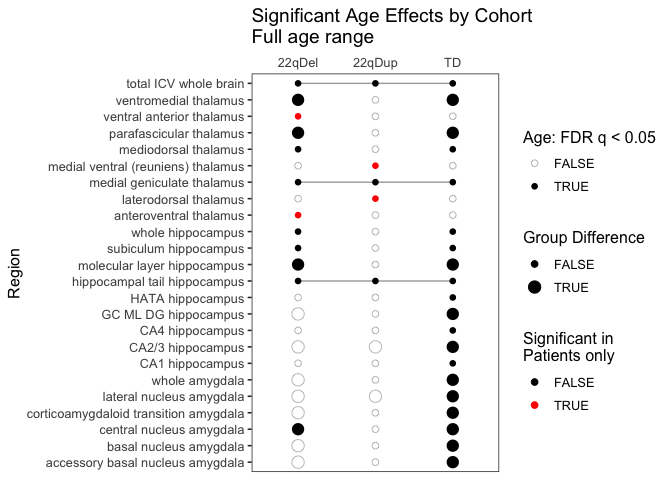
\includegraphics{22q_subcort_volumes_revised_files/figure-latex/unnamed-chunk-34-1.pdf}

\begin{Shaded}
\begin{Highlighting}[]
\CommentTok{\#ggsave(plot=maturation\_full$gamm\_compare+ggtitle("Significant Age Effects by Cohort\textbackslash{}nFull age range"), filename=file.path(project,"figures/age/age\_gamm\_group\_compare\_full.pdf"), width=7, height=5, device = "pdf")}
\CommentTok{\#ggsave(plot=maturation\_full$gamm\_compare+ggtitle("Significant Age Effects by Cohort\textbackslash{}nFull age range"), filename=file.path(project,"figures/age/age\_gamm\_group\_compare\_full.png"), width=7, height=5, device = "png", dpi = 300)}

\CommentTok{\# younger age range}
\NormalTok{maturation\_young}\SpecialCharTok{$}\NormalTok{gamm\_compare}\SpecialCharTok{+}\FunctionTok{ggtitle}\NormalTok{(}\StringTok{"Significant Age Effects by Cohort}\SpecialCharTok{\textbackslash{}n}\StringTok{Age \textless{} 35"}\NormalTok{)}
\end{Highlighting}
\end{Shaded}

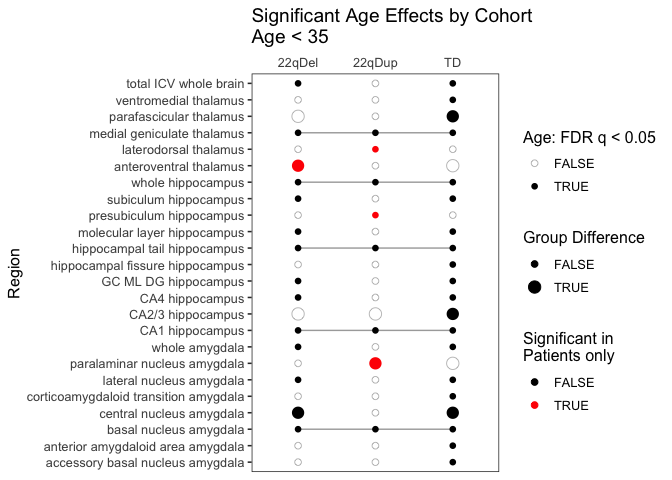
\includegraphics{22q_subcort_volumes_revised_files/figure-latex/unnamed-chunk-34-2.pdf}

\begin{Shaded}
\begin{Highlighting}[]
\CommentTok{\#ggsave(plot=maturation\_young$gamm\_compare+ggtitle("Significant Age Effects by Cohort\textbackslash{}nAge \textless{} 35"), filename=file.path(project,"figures/age/age\_gamm\_group\_compare\_u35.pdf"), width=7, height=5, device = "pdf")}
\CommentTok{\#ggsave(plot=maturation\_young$gamm\_compare+ggtitle("Significant Age Effects by Cohort\textbackslash{}nAge \textless{} 35"), filename=file.path(project,"figures/age/age\_gamm\_group\_compare\_u35.png"), width=7, height=5, device = "png", dpi = 300)}
\end{Highlighting}
\end{Shaded}

plot chosen GAMMS

\begin{Shaded}
\begin{Highlighting}[]
\CommentTok{\# function to plot all age smooths with partial residuals}
\NormalTok{plot\_gamm\_resid }\OtherTok{\textless{}{-}} \ControlFlowTok{function}\NormalTok{(list,name,}\AttributeTok{xlab=}\StringTok{""}\NormalTok{, }\AttributeTok{ylab=}\StringTok{""}\NormalTok{,}\AttributeTok{ylim=}\FunctionTok{c}\NormalTok{(}\SpecialCharTok{{-}}\DecValTok{1}\NormalTok{,}\DecValTok{1}\NormalTok{),}\AttributeTok{xlim=}\FunctionTok{c}\NormalTok{(}\FloatTok{5.9}\NormalTok{,}\DecValTok{23}\NormalTok{), }\AttributeTok{title=}\StringTok{""}\NormalTok{)\{}
\NormalTok{  gam\_list }\OtherTok{\textless{}{-}}\NormalTok{ list}\SpecialCharTok{$}\NormalTok{gam\_list}
\NormalTok{  smooth\_all\_combat }\OtherTok{\textless{}{-}}\NormalTok{ list}\SpecialCharTok{$}\NormalTok{smooth\_all\_combat}
  \ControlFlowTok{if}\NormalTok{(title}\SpecialCharTok{==}\StringTok{""}\NormalTok{)\{}
\NormalTok{    plot\_title }\OtherTok{\textless{}{-}} \FunctionTok{paste}\NormalTok{(}\FunctionTok{gsub}\NormalTok{(}\StringTok{"\_"}\NormalTok{,}\StringTok{" "}\NormalTok{,}\FunctionTok{gsub}\NormalTok{(}\StringTok{".combat.norm"}\NormalTok{,}\StringTok{""}\NormalTok{,name)),}\StringTok{"Volume"}\NormalTok{)}
\NormalTok{  \}}\ControlFlowTok{else}\NormalTok{\{}
\NormalTok{    plot\_title }\OtherTok{\textless{}{-}}\NormalTok{ title}
\NormalTok{  \}}
  \CommentTok{\#resid \textless{}{-} add\_partial\_residuals(data=demo\_combat\_na,model=gam\_list[[name]])}
\NormalTok{  resid }\OtherTok{\textless{}{-}} \FunctionTok{add\_partial\_residuals}\NormalTok{(}\AttributeTok{data=}\NormalTok{gam\_list[[name]]}\SpecialCharTok{$}\NormalTok{model,}\AttributeTok{model=}\NormalTok{gam\_list[[name]])}
\NormalTok{  resid\_del }\OtherTok{\textless{}{-}} \FunctionTok{filter}\NormalTok{(resid, SUBJECT\_IDENTITY}\SpecialCharTok{==}\StringTok{"PATIENT{-}DEL"}\NormalTok{)}
\NormalTok{  resid\_del}\SpecialCharTok{$}\NormalTok{yvar }\OtherTok{\textless{}{-}}\NormalTok{ resid\_del}\SpecialCharTok{$}\StringTok{\textasciigrave{}}\AttributeTok{s(AGE):SUBJECT\_IDENTITYPATIENT{-}DEL}\StringTok{\textasciigrave{}}
\NormalTok{  resid\_dup }\OtherTok{\textless{}{-}} \FunctionTok{filter}\NormalTok{(resid, SUBJECT\_IDENTITY}\SpecialCharTok{==}\StringTok{"PATIENT{-}DUP"}\NormalTok{)}
\NormalTok{  resid\_dup}\SpecialCharTok{$}\NormalTok{yvar }\OtherTok{\textless{}{-}}\NormalTok{ resid\_dup}\SpecialCharTok{$}\StringTok{\textasciigrave{}}\AttributeTok{s(AGE):SUBJECT\_IDENTITYPATIENT{-}DUP}\StringTok{\textasciigrave{}}
\NormalTok{  resid\_hcs }\OtherTok{\textless{}{-}} \FunctionTok{filter}\NormalTok{(resid, SUBJECT\_IDENTITY}\SpecialCharTok{==}\StringTok{"CONTROL"}\NormalTok{)}
\NormalTok{  resid\_hcs}\SpecialCharTok{$}\NormalTok{yvar }\OtherTok{\textless{}{-}}\NormalTok{ resid\_hcs}\SpecialCharTok{$}\StringTok{\textasciigrave{}}\AttributeTok{s(AGE):SUBJECT\_IDENTITYCONTROL}\StringTok{\textasciigrave{}}
  \FunctionTok{ggplot}\NormalTok{()}\SpecialCharTok{+}
    \FunctionTok{geom\_point}\NormalTok{(}\AttributeTok{data=}\NormalTok{resid\_del, }\FunctionTok{aes}\NormalTok{(}\AttributeTok{x=}\NormalTok{AGE, }\AttributeTok{y=}\NormalTok{yvar), }\AttributeTok{alpha=}\FloatTok{0.8}\NormalTok{,}\AttributeTok{shape=}\DecValTok{21}\NormalTok{, }\AttributeTok{color=}\StringTok{"gray20"}\NormalTok{, }\AttributeTok{fill=}\FunctionTok{viridis}\NormalTok{(}\DecValTok{3}\NormalTok{)[}\DecValTok{1}\NormalTok{]) }\SpecialCharTok{+}
    \FunctionTok{geom\_line}\NormalTok{(}\AttributeTok{data=}\NormalTok{resid\_del, }\FunctionTok{aes}\NormalTok{(}\AttributeTok{x=}\NormalTok{AGE, }\AttributeTok{y=}\NormalTok{yvar, }\AttributeTok{group=}\NormalTok{SUBJECTID), }\AttributeTok{alpha=}\FloatTok{0.6}\NormalTok{,}\AttributeTok{shape=}\DecValTok{21}\NormalTok{, }\AttributeTok{color=}\FunctionTok{viridis}\NormalTok{(}\DecValTok{3}\NormalTok{)[}\DecValTok{1}\NormalTok{])}\SpecialCharTok{+}
    \FunctionTok{geom\_point}\NormalTok{(}\AttributeTok{data=}\NormalTok{resid\_hcs, }\FunctionTok{aes}\NormalTok{(}\AttributeTok{x=}\NormalTok{AGE, }\AttributeTok{y=}\NormalTok{yvar), }\AttributeTok{alpha=}\FloatTok{0.8}\NormalTok{, }\AttributeTok{shape=}\DecValTok{21}\NormalTok{, }\AttributeTok{color=}\StringTok{"gray20"}\NormalTok{, }\AttributeTok{fill=}\FunctionTok{viridis}\NormalTok{(}\DecValTok{3}\NormalTok{)[}\DecValTok{2}\NormalTok{]) }\SpecialCharTok{+}
    \FunctionTok{geom\_line}\NormalTok{(}\AttributeTok{data=}\NormalTok{resid\_hcs, }\FunctionTok{aes}\NormalTok{(}\AttributeTok{x=}\NormalTok{AGE, }\AttributeTok{y=}\NormalTok{yvar, }\AttributeTok{group=}\NormalTok{SUBJECTID), }\AttributeTok{alpha=}\FloatTok{0.6}\NormalTok{,}\AttributeTok{shape=}\DecValTok{21}\NormalTok{, }\AttributeTok{color=}\FunctionTok{viridis}\NormalTok{(}\DecValTok{3}\NormalTok{)[}\DecValTok{2}\NormalTok{])}\SpecialCharTok{+}
    \FunctionTok{geom\_point}\NormalTok{(}\AttributeTok{data=}\NormalTok{resid\_dup, }\FunctionTok{aes}\NormalTok{(}\AttributeTok{x=}\NormalTok{AGE, }\AttributeTok{y=}\NormalTok{yvar), }\AttributeTok{alpha=}\FloatTok{0.8}\NormalTok{, }\AttributeTok{shape=}\DecValTok{21}\NormalTok{, }\AttributeTok{color=}\StringTok{"gray20"}\NormalTok{, }\AttributeTok{fill=}\FunctionTok{viridis}\NormalTok{(}\DecValTok{3}\NormalTok{)[}\DecValTok{3}\NormalTok{]) }\SpecialCharTok{+}
    \FunctionTok{geom\_line}\NormalTok{(}\AttributeTok{data=}\NormalTok{resid\_dup, }\FunctionTok{aes}\NormalTok{(}\AttributeTok{x=}\NormalTok{AGE, }\AttributeTok{y=}\NormalTok{yvar, }\AttributeTok{group=}\NormalTok{SUBJECTID), }\AttributeTok{alpha=}\FloatTok{0.8}\NormalTok{,}\AttributeTok{shape=}\DecValTok{21}\NormalTok{, }\AttributeTok{color=}\StringTok{"orange"}\NormalTok{)}\SpecialCharTok{+}
    \CommentTok{\#scale\_shape\_manual(values = c(17, 16))+}
    \CommentTok{\# td }
    \FunctionTok{geom\_ribbon}\NormalTok{(}\AttributeTok{data =} \FunctionTok{filter}\NormalTok{(smooth\_all\_combat[[name]], SUBJECT\_IDENTITY}\SpecialCharTok{==}\StringTok{"CONTROL"}\NormalTok{),}
                \FunctionTok{aes}\NormalTok{(}\AttributeTok{x =}\NormalTok{ AGE, }\AttributeTok{ymin =}\NormalTok{ selo,}\AttributeTok{ymax =}\NormalTok{ sehi, }\AttributeTok{fill =}\NormalTok{ SUBJECT\_IDENTITY),}\AttributeTok{alpha =}\NormalTok{ .}\DecValTok{3}\NormalTok{, }\AttributeTok{linetype =} \DecValTok{0}\NormalTok{)}\SpecialCharTok{+}
    \FunctionTok{geom\_line}\NormalTok{(}\AttributeTok{data =} \FunctionTok{filter}\NormalTok{(smooth\_all\_combat[[name]], SUBJECT\_IDENTITY}\SpecialCharTok{==}\StringTok{"CONTROL"}\NormalTok{),}
              \FunctionTok{aes}\NormalTok{(}\AttributeTok{x =}\NormalTok{ AGE, }\AttributeTok{y =}\NormalTok{ est, }\AttributeTok{color =}\NormalTok{ SUBJECT\_IDENTITY),}\AttributeTok{size =} \DecValTok{1}\NormalTok{)}\SpecialCharTok{+}\FunctionTok{theme\_bw}\NormalTok{()}\SpecialCharTok{+}
    \CommentTok{\# dup}
    \FunctionTok{geom\_ribbon}\NormalTok{(}\AttributeTok{data =} \FunctionTok{filter}\NormalTok{(smooth\_all\_combat[[name]], SUBJECT\_IDENTITY}\SpecialCharTok{==}\StringTok{"PATIENT{-}DUP"}\NormalTok{),}
                \FunctionTok{aes}\NormalTok{(}\AttributeTok{x =}\NormalTok{ AGE, }\AttributeTok{ymin =}\NormalTok{ selo,}\AttributeTok{ymax =}\NormalTok{ sehi, }\AttributeTok{fill =}\NormalTok{ SUBJECT\_IDENTITY),}\AttributeTok{alpha =}\NormalTok{ .}\DecValTok{6}\NormalTok{, }\AttributeTok{linetype =} \DecValTok{0}\NormalTok{)}\SpecialCharTok{+}
    \FunctionTok{geom\_line}\NormalTok{(}\AttributeTok{data =} \FunctionTok{filter}\NormalTok{(smooth\_all\_combat[[name]], SUBJECT\_IDENTITY}\SpecialCharTok{==}\StringTok{"PATIENT{-}DUP"}\NormalTok{),}
              \FunctionTok{aes}\NormalTok{(}\AttributeTok{x =}\NormalTok{ AGE, }\AttributeTok{y =}\NormalTok{ est, }\AttributeTok{color =}\NormalTok{ SUBJECT\_IDENTITY),}\AttributeTok{size =} \DecValTok{1}\NormalTok{)}\SpecialCharTok{+}\FunctionTok{theme\_bw}\NormalTok{()}\SpecialCharTok{+}
    \CommentTok{\# del}
    \FunctionTok{geom\_ribbon}\NormalTok{(}\AttributeTok{data =} \FunctionTok{filter}\NormalTok{(smooth\_all\_combat[[name]], SUBJECT\_IDENTITY}\SpecialCharTok{==}\StringTok{"PATIENT{-}DEL"}\NormalTok{),}
                \FunctionTok{aes}\NormalTok{(}\AttributeTok{x =}\NormalTok{ AGE, }\AttributeTok{ymin =}\NormalTok{ selo,}\AttributeTok{ymax =}\NormalTok{ sehi, }\AttributeTok{fill =}\NormalTok{ SUBJECT\_IDENTITY),}\AttributeTok{alpha =}\NormalTok{ .}\DecValTok{3}\NormalTok{, }\AttributeTok{linetype =} \DecValTok{0}\NormalTok{)}\SpecialCharTok{+}
    \FunctionTok{geom\_line}\NormalTok{(}\AttributeTok{data =} \FunctionTok{filter}\NormalTok{(smooth\_all\_combat[[name]], SUBJECT\_IDENTITY}\SpecialCharTok{==}\StringTok{"PATIENT{-}DEL"}\NormalTok{),}
              \FunctionTok{aes}\NormalTok{(}\AttributeTok{x =}\NormalTok{ AGE, }\AttributeTok{y =}\NormalTok{ est, }\AttributeTok{color =}\NormalTok{ SUBJECT\_IDENTITY),}\AttributeTok{size =} \DecValTok{1}\NormalTok{)}\SpecialCharTok{+}\FunctionTok{theme\_bw}\NormalTok{()}\SpecialCharTok{+}
    \CommentTok{\#scale\_fill\_manual(values = c("CONTROL" = viridis(3)[2], "PATIENT{-}DEL" = viridis(3)[1], "PATIENT{-}DUP" ="black"), labels=c("Control","22qDel","22qDup")) +}
    \FunctionTok{scale\_fill\_manual}\NormalTok{(}\AttributeTok{values =} \FunctionTok{c}\NormalTok{(}\StringTok{"CONTROL"} \OtherTok{=} \FunctionTok{viridis}\NormalTok{(}\DecValTok{3}\NormalTok{)[}\DecValTok{2}\NormalTok{], }\StringTok{"PATIENT{-}DEL"} \OtherTok{=} \FunctionTok{viridis}\NormalTok{(}\DecValTok{3}\NormalTok{)[}\DecValTok{1}\NormalTok{], }\StringTok{"PATIENT{-}DUP"} \OtherTok{=}\FunctionTok{viridis}\NormalTok{(}\DecValTok{3}\NormalTok{)[}\DecValTok{3}\NormalTok{]), }\AttributeTok{labels=}\FunctionTok{c}\NormalTok{(}\StringTok{"Control"}\NormalTok{,}\StringTok{"22qDel"}\NormalTok{,}\StringTok{"22qDup"}\NormalTok{)) }\SpecialCharTok{+}
    \FunctionTok{scale\_color\_manual}\NormalTok{(}\AttributeTok{values =} \FunctionTok{c}\NormalTok{(}\StringTok{"CONTROL"} \OtherTok{=} \FunctionTok{viridis}\NormalTok{(}\DecValTok{3}\NormalTok{)[}\DecValTok{2}\NormalTok{], }\StringTok{"PATIENT{-}DEL"} \OtherTok{=} \FunctionTok{viridis}\NormalTok{(}\DecValTok{3}\NormalTok{)[}\DecValTok{1}\NormalTok{], }\StringTok{"PATIENT{-}DUP"} \OtherTok{=}\StringTok{"orange"}\NormalTok{), }\AttributeTok{labels=}\FunctionTok{c}\NormalTok{(}\StringTok{"Control"}\NormalTok{,}\StringTok{"22qDel"}\NormalTok{,}\StringTok{"22qDup"}\NormalTok{)) }\SpecialCharTok{+}
    \CommentTok{\#scale\_x\_continuous(limits=xlim,expand=c(0,0))+}
    \CommentTok{\#scale\_y\_continuous(limits=ylim,expand=c(0,0))+}
    \FunctionTok{theme\_classic}\NormalTok{() }\SpecialCharTok{+} 
    \FunctionTok{theme}\NormalTok{(}\AttributeTok{legend.title =} \FunctionTok{element\_blank}\NormalTok{())}\SpecialCharTok{+}
    \FunctionTok{theme}\NormalTok{(}\AttributeTok{axis.title.y =} \FunctionTok{element\_text}\NormalTok{(}\AttributeTok{angle =} \DecValTok{0}\NormalTok{,}\AttributeTok{vjust=}\FloatTok{0.5}\NormalTok{))}\SpecialCharTok{+}
    \FunctionTok{ylab}\NormalTok{(ylab)}\SpecialCharTok{+}
    \FunctionTok{xlab}\NormalTok{(xlab)}\SpecialCharTok{+}
    \CommentTok{\#ggtitle(paste(gsub("\_"," ",gsub(".combat","",name)),"Volume"))}
    \FunctionTok{ggtitle}\NormalTok{(plot\_title)}
\NormalTok{\}}
\end{Highlighting}
\end{Shaded}

\begin{Shaded}
\begin{Highlighting}[]
\CommentTok{\# function to plot all age smooths with age ranges of significant difference from controls highlighted}
\NormalTok{plot\_gamm\_gdiff }\OtherTok{\textless{}{-}} \ControlFlowTok{function}\NormalTok{(list,name,}\AttributeTok{xlab=}\StringTok{""}\NormalTok{, }\AttributeTok{ylab=}\StringTok{""}\NormalTok{,}\AttributeTok{ylim=}\FunctionTok{c}\NormalTok{(}\SpecialCharTok{{-}}\DecValTok{1}\NormalTok{,}\DecValTok{1}\NormalTok{),}\AttributeTok{xlim=}\FunctionTok{c}\NormalTok{(}\FloatTok{5.9}\NormalTok{,}\DecValTok{23}\NormalTok{), }\AttributeTok{title=}\StringTok{""}\NormalTok{)\{}
\NormalTok{  gam\_list }\OtherTok{\textless{}{-}}\NormalTok{ list}\SpecialCharTok{$}\NormalTok{gam\_list}
\NormalTok{  smooth\_all\_gdiff }\OtherTok{\textless{}{-}}\NormalTok{ list}\SpecialCharTok{$}\NormalTok{smooth\_all\_gdiff}
\NormalTok{  smooth\_sig\_gdiff }\OtherTok{\textless{}{-}}\NormalTok{ list}\SpecialCharTok{$}\NormalTok{smooth\_sig\_gdiff}
  \ControlFlowTok{if}\NormalTok{(title}\SpecialCharTok{==}\StringTok{""}\NormalTok{)\{}
\NormalTok{    plot\_title }\OtherTok{\textless{}{-}} \FunctionTok{paste}\NormalTok{(}\FunctionTok{gsub}\NormalTok{(}\StringTok{"\_"}\NormalTok{,}\StringTok{" "}\NormalTok{,}\FunctionTok{gsub}\NormalTok{(}\StringTok{".combat.norm"}\NormalTok{,}\StringTok{""}\NormalTok{,name)),}\StringTok{"Volume"}\NormalTok{)}
\NormalTok{  \}}\ControlFlowTok{else}\NormalTok{\{}
\NormalTok{    plot\_title }\OtherTok{\textless{}{-}}\NormalTok{ title}
\NormalTok{  \}}
  \FunctionTok{ggplot}\NormalTok{()}\SpecialCharTok{+}
    \CommentTok{\# td }
    \FunctionTok{geom\_ribbon}\NormalTok{(}\AttributeTok{data =} \FunctionTok{filter}\NormalTok{(smooth\_all\_gdiff[[name]], SUBJECT\_IDENTITY}\SpecialCharTok{==}\StringTok{"CONTROL"}\NormalTok{),}
                \FunctionTok{aes}\NormalTok{(}\AttributeTok{x =}\NormalTok{ AGE, }\AttributeTok{ymin =}\NormalTok{ selo,}\AttributeTok{ymax =}\NormalTok{ sehi, }\AttributeTok{fill =}\NormalTok{ SUBJECT\_IDENTITY),}\AttributeTok{alpha =}\NormalTok{ .}\DecValTok{3}\NormalTok{, }\AttributeTok{linetype =} \DecValTok{0}\NormalTok{)}\SpecialCharTok{+}
    \FunctionTok{geom\_line}\NormalTok{(}\AttributeTok{data =} \FunctionTok{filter}\NormalTok{(smooth\_all\_gdiff[[name]], SUBJECT\_IDENTITY}\SpecialCharTok{==}\StringTok{"CONTROL"}\NormalTok{),}
              \FunctionTok{aes}\NormalTok{(}\AttributeTok{x =}\NormalTok{ AGE, }\AttributeTok{y =}\NormalTok{ est, }\AttributeTok{color =}\NormalTok{ SUBJECT\_IDENTITY),}\AttributeTok{size =} \FloatTok{0.5}\NormalTok{)}\SpecialCharTok{+}\FunctionTok{theme\_bw}\NormalTok{()}\SpecialCharTok{+}
    \CommentTok{\# dup}
    \FunctionTok{geom\_ribbon}\NormalTok{(}\AttributeTok{data =} \FunctionTok{filter}\NormalTok{(smooth\_all\_gdiff[[name]], SUBJECT\_IDENTITY}\SpecialCharTok{==}\StringTok{"PATIENT{-}DUP"}\NormalTok{),}
                \FunctionTok{aes}\NormalTok{(}\AttributeTok{x =}\NormalTok{ AGE, }\AttributeTok{ymin =}\NormalTok{ selo,}\AttributeTok{ymax =}\NormalTok{ sehi, }\AttributeTok{fill =}\NormalTok{ SUBJECT\_IDENTITY),}\AttributeTok{alpha =}\NormalTok{ .}\DecValTok{6}\NormalTok{, }\AttributeTok{linetype =} \DecValTok{0}\NormalTok{)}\SpecialCharTok{+}
    \FunctionTok{geom\_line}\NormalTok{(}\AttributeTok{data =} \FunctionTok{filter}\NormalTok{(smooth\_all\_gdiff[[name]], SUBJECT\_IDENTITY}\SpecialCharTok{==}\StringTok{"PATIENT{-}DUP"}\NormalTok{),}
              \FunctionTok{aes}\NormalTok{(}\AttributeTok{x =}\NormalTok{ AGE, }\AttributeTok{y =}\NormalTok{ est, }\AttributeTok{color =}\NormalTok{ SUBJECT\_IDENTITY),}\AttributeTok{size =} \FloatTok{0.5}\NormalTok{)}\SpecialCharTok{+}\FunctionTok{theme\_bw}\NormalTok{()}\SpecialCharTok{+}
    \FunctionTok{geom\_line}\NormalTok{(}\AttributeTok{data =} \FunctionTok{filter}\NormalTok{(smooth\_sig\_gdiff[[name]], SUBJECT\_IDENTITY}\SpecialCharTok{==}\StringTok{"PATIENT{-}DUP"}\NormalTok{),}
              \FunctionTok{aes}\NormalTok{(}\AttributeTok{x =}\NormalTok{ AGE, }\AttributeTok{y =}\NormalTok{ est, }\AttributeTok{color =}\NormalTok{ SUBJECT\_IDENTITY),}\AttributeTok{size =} \FloatTok{1.5}\NormalTok{)}\SpecialCharTok{+}\FunctionTok{theme\_bw}\NormalTok{()}\SpecialCharTok{+}
    \CommentTok{\# geom\_point(data = filter(smooth\_all\_gdiff[[name]], SUBJECT\_IDENTITY=="PATIENT{-}DUP" \& gdiff == TRUE),}
    \CommentTok{\#           aes(x = AGE, y = est),color = "orange",size = 1, alpha=1)+theme\_bw()+}
    \CommentTok{\# del}
    \FunctionTok{geom\_ribbon}\NormalTok{(}\AttributeTok{data =} \FunctionTok{filter}\NormalTok{(smooth\_all\_gdiff[[name]], SUBJECT\_IDENTITY}\SpecialCharTok{==}\StringTok{"PATIENT{-}DEL"}\NormalTok{),}
                \FunctionTok{aes}\NormalTok{(}\AttributeTok{x =}\NormalTok{ AGE, }\AttributeTok{ymin =}\NormalTok{ selo,}\AttributeTok{ymax =}\NormalTok{ sehi, }\AttributeTok{fill =}\NormalTok{ SUBJECT\_IDENTITY),}\AttributeTok{alpha =}\NormalTok{ .}\DecValTok{3}\NormalTok{, }\AttributeTok{linetype =} \DecValTok{0}\NormalTok{)}\SpecialCharTok{+}
    \FunctionTok{geom\_line}\NormalTok{(}\AttributeTok{data =} \FunctionTok{filter}\NormalTok{(smooth\_all\_gdiff[[name]], SUBJECT\_IDENTITY}\SpecialCharTok{==}\StringTok{"PATIENT{-}DEL"}\NormalTok{),}
              \FunctionTok{aes}\NormalTok{(}\AttributeTok{x =}\NormalTok{ AGE, }\AttributeTok{y =}\NormalTok{ est, }\AttributeTok{color =}\NormalTok{ SUBJECT\_IDENTITY),}\AttributeTok{size =} \FloatTok{0.5}\NormalTok{, }\AttributeTok{na.rm =} \ConstantTok{TRUE}\NormalTok{)}\SpecialCharTok{+}\FunctionTok{theme\_bw}\NormalTok{()}\SpecialCharTok{+}
    \FunctionTok{geom\_line}\NormalTok{(}\AttributeTok{data =} \FunctionTok{filter}\NormalTok{(smooth\_sig\_gdiff[[name]], SUBJECT\_IDENTITY}\SpecialCharTok{==}\StringTok{"PATIENT{-}DEL"}\NormalTok{),}
              \FunctionTok{aes}\NormalTok{(}\AttributeTok{x =}\NormalTok{ AGE, }\AttributeTok{y =}\NormalTok{ est, }\AttributeTok{color =}\NormalTok{ SUBJECT\_IDENTITY),}\AttributeTok{size =} \FloatTok{1.5}\NormalTok{, }\AttributeTok{na.rm =} \ConstantTok{TRUE}\NormalTok{)}\SpecialCharTok{+}\FunctionTok{theme\_bw}\NormalTok{()}\SpecialCharTok{+}
    \CommentTok{\# geom\_point(data = filter(smooth\_all\_gdiff[[name]], SUBJECT\_IDENTITY=="PATIENT{-}DEL" \& gdiff == TRUE),}
    \CommentTok{\#           aes(x = AGE, y = est, color=SUBJECT\_IDENTITY),shape=19, color = "blue",size = 1, alpha=1)+theme\_bw()+}
    \CommentTok{\#scale\_fill\_manual(values = c("CONTROL" = viridis(3)[2], "PATIENT{-}DEL" = viridis(3)[1], "PATIENT{-}DUP" ="black"), labels=c("Control","22qDel","22qDup")) +}
    \FunctionTok{scale\_fill\_manual}\NormalTok{(}\AttributeTok{values =} \FunctionTok{c}\NormalTok{(}\StringTok{"CONTROL"} \OtherTok{=} \FunctionTok{viridis}\NormalTok{(}\DecValTok{3}\NormalTok{)[}\DecValTok{2}\NormalTok{], }\StringTok{"PATIENT{-}DEL"} \OtherTok{=} \FunctionTok{viridis}\NormalTok{(}\DecValTok{3}\NormalTok{)[}\DecValTok{1}\NormalTok{], }\StringTok{"PATIENT{-}DUP"} \OtherTok{=}\FunctionTok{viridis}\NormalTok{(}\DecValTok{3}\NormalTok{)[}\DecValTok{3}\NormalTok{]), }\AttributeTok{labels=}\FunctionTok{c}\NormalTok{(}\StringTok{"Control"}\NormalTok{,}\StringTok{"22qDel"}\NormalTok{,}\StringTok{"22qDup"}\NormalTok{)) }\SpecialCharTok{+}
    \CommentTok{\#scale\_color\_manual(values = c("CONTROL" = viridis(3)[2], "PATIENT{-}DEL" = viridis(3)[1], "PATIENT{-}DUP" = viridis(3)[3]), labels=c("Control","22qDel","22qDup")) +}
    \FunctionTok{scale\_color\_manual}\NormalTok{(}\AttributeTok{values =} \FunctionTok{c}\NormalTok{(}\StringTok{"CONTROL"} \OtherTok{=} \FunctionTok{viridis}\NormalTok{(}\DecValTok{3}\NormalTok{)[}\DecValTok{2}\NormalTok{], }\StringTok{"PATIENT{-}DEL"} \OtherTok{=} \FunctionTok{viridis}\NormalTok{(}\DecValTok{3}\NormalTok{)[}\DecValTok{1}\NormalTok{], }\StringTok{"PATIENT{-}DUP"} \OtherTok{=} \StringTok{"orange"}\NormalTok{), }\AttributeTok{labels=}\FunctionTok{c}\NormalTok{(}\StringTok{"Control"}\NormalTok{,}\StringTok{"22qDel"}\NormalTok{,}\StringTok{"22qDup"}\NormalTok{)) }\SpecialCharTok{+}
    \CommentTok{\#scale\_x\_continuous(limits=xlim,expand=c(0,0))+}
    \CommentTok{\#scale\_y\_continuous(limits=ylim,expand=c(0,0))+}
    \FunctionTok{theme\_classic}\NormalTok{() }\SpecialCharTok{+} 
    \FunctionTok{theme}\NormalTok{(}\AttributeTok{legend.title =} \FunctionTok{element\_blank}\NormalTok{())}\SpecialCharTok{+}
    \FunctionTok{theme}\NormalTok{(}\AttributeTok{axis.title.y =} \FunctionTok{element\_text}\NormalTok{(}\AttributeTok{angle =} \DecValTok{0}\NormalTok{,}\AttributeTok{vjust=}\FloatTok{0.5}\NormalTok{))}\SpecialCharTok{+}
    \FunctionTok{ylab}\NormalTok{(ylab)}\SpecialCharTok{+}
    \FunctionTok{xlab}\NormalTok{(xlab)}\SpecialCharTok{+}
    \CommentTok{\#ggtitle(paste(gsub("\_"," ",gsub(".combat","",name)),"Volume"))}
    \FunctionTok{ggtitle}\NormalTok{(plot\_title)}
\NormalTok{\}}

\CommentTok{\#plot\_gamm\_gdiff(list=mat\_full\_gdiff, name="Hip\_CA3.combat.norm",xlab="",ylab="", title="CA2/3 Hippocampus")}
\end{Highlighting}
\end{Shaded}

plot age gamms with partial resids for full sample

\begin{Shaded}
\begin{Highlighting}[]
\CommentTok{\#plot chosen gamms}
\NormalTok{thal\_av }\OtherTok{\textless{}{-}} \FunctionTok{plot\_gamm\_resid}\NormalTok{(}\AttributeTok{list=}\NormalTok{maturation\_full, }\AttributeTok{name=}\StringTok{"Thal\_AV.combat.norm"}\NormalTok{,}\AttributeTok{xlab=}\StringTok{"Age"}\NormalTok{,}\AttributeTok{ylab=}\StringTok{"Normalized}\SpecialCharTok{\textbackslash{}n}\StringTok{Volume"}\NormalTok{, }\AttributeTok{title=}\StringTok{"Anteroventral Thalamus"}\NormalTok{)}
\NormalTok{hip\_ca3 }\OtherTok{\textless{}{-}} \FunctionTok{plot\_gamm\_resid}\NormalTok{(}\AttributeTok{list=}\NormalTok{maturation\_full, }\AttributeTok{name=}\StringTok{"Hip\_CA3.combat.norm"}\NormalTok{,}\AttributeTok{xlab=}\StringTok{""}\NormalTok{,}\AttributeTok{ylab=}\StringTok{""}\NormalTok{, }\AttributeTok{title=}\StringTok{"CA2/3 Hippocampus"}\NormalTok{)}
\NormalTok{amy\_whole }\OtherTok{\textless{}{-}} \FunctionTok{plot\_gamm\_resid}\NormalTok{(}\AttributeTok{list=}\NormalTok{maturation\_full, }\AttributeTok{name=}\StringTok{"Amy\_Whole\_amygdala.combat.norm"}\NormalTok{,}\AttributeTok{xlab=}\StringTok{""}\NormalTok{,}\AttributeTok{ylab=}\StringTok{""}\NormalTok{, }\AttributeTok{title=}\StringTok{"Whole Amygdala"}\NormalTok{)}
\NormalTok{thal\_mgn }\OtherTok{\textless{}{-}} \FunctionTok{plot\_gamm\_resid}\NormalTok{(}\AttributeTok{list=}\NormalTok{maturation\_full, }\AttributeTok{name=}\StringTok{"Thal\_MGN.combat.norm"}\NormalTok{,}\AttributeTok{xlab=}\StringTok{""}\NormalTok{,}\AttributeTok{ylab=}\StringTok{""}\NormalTok{, }\AttributeTok{title=}\StringTok{"Medial Geniculate Thalamus"}\NormalTok{)}
\NormalTok{thal\_mvre }\OtherTok{\textless{}{-}} \FunctionTok{plot\_gamm\_resid}\NormalTok{(}\AttributeTok{list=}\NormalTok{maturation\_full, }\AttributeTok{name=}\StringTok{"Thal\_MV\_Re\_.combat.norm"}\NormalTok{,}\AttributeTok{xlab=}\StringTok{""}\NormalTok{,}\AttributeTok{ylab=}\StringTok{""}\NormalTok{, }\AttributeTok{title=}\StringTok{"Medial Ventral Thalamus"}\NormalTok{)}
\NormalTok{hip\_ca4 }\OtherTok{\textless{}{-}} \FunctionTok{plot\_gamm\_resid}\NormalTok{(}\AttributeTok{list=}\NormalTok{maturation\_full, }\AttributeTok{name=}\StringTok{"Hip\_CA4.combat.norm"}\NormalTok{,}\AttributeTok{xlab=}\StringTok{""}\NormalTok{,}\AttributeTok{ylab=}\StringTok{""}\NormalTok{, }\AttributeTok{title=}\StringTok{"CA4 Hippocampus"}\NormalTok{)}
\CommentTok{\#amy\_aaa \textless{}{-} plot\_gamm\_resid(name="Amy\_Anterior\_amygdaloid\_area\_AAA.combat.norm",xlab="Age",ylab="Volume")}
\CommentTok{\#thal\_lgn \textless{}{-} plot\_gamm\_resid(name="Thal\_LGN.combat.norm",xlab="Age",ylab="Volume")}
\CommentTok{\#thal\_mgn \textless{}{-} plot\_gamm\_resid(name="Thal\_MGN.combat.norm",xlab="Age",ylab="Volume")}
\CommentTok{\#hip\_ca1 \textless{}{-} plot\_gamm\_resid(name="Hip\_CA1.combat.norm",xlab="",ylab="", title="CA1 Hippocampus")}


\NormalTok{plot\_age }\OtherTok{\textless{}{-}}\NormalTok{ (thal\_av }\SpecialCharTok{+}\NormalTok{ hip\_ca3 }\SpecialCharTok{+}\NormalTok{ hip\_ca4) }\SpecialCharTok{/}\NormalTok{ (thal\_mgn }\SpecialCharTok{+}\NormalTok{ thal\_mvre }\SpecialCharTok{+}\NormalTok{ amy\_whole) }\SpecialCharTok{+} \FunctionTok{plot\_layout}\NormalTok{(}\AttributeTok{guides =} \StringTok{"collect"}\NormalTok{) }\SpecialCharTok{+} \FunctionTok{plot\_annotation}\NormalTok{(}\AttributeTok{tag\_levels =} \StringTok{\textquotesingle{}A\textquotesingle{}}\NormalTok{, }\AttributeTok{title=}\StringTok{"Developmental Trajectories}\SpecialCharTok{\textbackslash{}n}\StringTok{Full age range"}\NormalTok{) }\SpecialCharTok{\&}   \FunctionTok{theme}\NormalTok{(}\AttributeTok{plot.tag =} \FunctionTok{element\_text}\NormalTok{(}\AttributeTok{face =} \StringTok{\textquotesingle{}bold\textquotesingle{}}\NormalTok{)) }\SpecialCharTok{+} \FunctionTok{theme}\NormalTok{(}\AttributeTok{legend.position =} \StringTok{"bottom"}\NormalTok{, }\AttributeTok{legend.text=}\FunctionTok{element\_text}\NormalTok{(}\AttributeTok{size=}\DecValTok{14}\NormalTok{), }\AttributeTok{plot.title =} \FunctionTok{element\_text}\NormalTok{(}\AttributeTok{size=}\DecValTok{16}\NormalTok{, }\AttributeTok{hjust =} \DecValTok{0}\NormalTok{)) }

\NormalTok{plot\_age}
\end{Highlighting}
\end{Shaded}

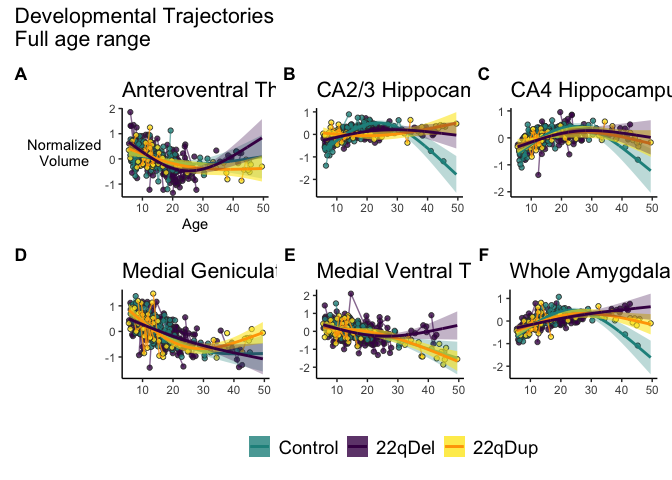
\includegraphics{22q_subcort_volumes_revised_files/figure-latex/unnamed-chunk-37-1.pdf}

\begin{Shaded}
\begin{Highlighting}[]
\CommentTok{\#ggsave(plot=plot\_age, filename=file.path(project,"figures/age/age\_gamms\_curves\_resid\_full.pdf"), width=12, height=7, device = "pdf")}
\CommentTok{\#ggsave(plot=plot\_age, filename=file.path(project,"figures/age/age\_gamms\_curves\_resid\_full.png"), width=12, height=7, device = "png", dpi = 300)}
\end{Highlighting}
\end{Shaded}

plot age gamms with group differences for full sample

\begin{Shaded}
\begin{Highlighting}[]
\CommentTok{\#plot chosen gamms}
\NormalTok{thal\_av\_gd }\OtherTok{\textless{}{-}} \FunctionTok{plot\_gamm\_gdiff}\NormalTok{(}\AttributeTok{list=}\NormalTok{mat\_full\_gdiff, }\AttributeTok{name=}\StringTok{"Thal\_AV.combat.norm"}\NormalTok{,}\AttributeTok{xlab=}\StringTok{"Age"}\NormalTok{,}\AttributeTok{ylab=}\StringTok{"Normalized}\SpecialCharTok{\textbackslash{}n}\StringTok{Volume"}\NormalTok{, }\AttributeTok{title=}\StringTok{"Anteroventral Thalamus"}\NormalTok{)}
\NormalTok{hip\_ca3\_gd }\OtherTok{\textless{}{-}} \FunctionTok{plot\_gamm\_gdiff}\NormalTok{(}\AttributeTok{list=}\NormalTok{mat\_full\_gdiff, }\AttributeTok{name=}\StringTok{"Hip\_CA3.combat.norm"}\NormalTok{,}\AttributeTok{xlab=}\StringTok{""}\NormalTok{,}\AttributeTok{ylab=}\StringTok{""}\NormalTok{, }\AttributeTok{title=}\StringTok{"CA2/3 Hippocampus"}\NormalTok{)}
\NormalTok{amy\_whole\_gd }\OtherTok{\textless{}{-}} \FunctionTok{plot\_gamm\_gdiff}\NormalTok{(}\AttributeTok{list=}\NormalTok{mat\_full\_gdiff, }\AttributeTok{name=}\StringTok{"Amy\_Whole\_amygdala.combat.norm"}\NormalTok{,}\AttributeTok{xlab=}\StringTok{""}\NormalTok{,}\AttributeTok{ylab=}\StringTok{""}\NormalTok{, }\AttributeTok{title=}\StringTok{"Whole Amygdala"}\NormalTok{)}
\CommentTok{\#thal\_md\_gd \textless{}{-} plot\_gamm\_gdiff(list=mat\_full\_gdiff, name="Thal\_MD\_all.combat.norm",xlab="",ylab="", title="Mediodorsal Thalamus")}
\NormalTok{thal\_mgn\_gd }\OtherTok{\textless{}{-}} \FunctionTok{plot\_gamm\_gdiff}\NormalTok{(}\AttributeTok{list=}\NormalTok{mat\_full\_gdiff, }\AttributeTok{name=}\StringTok{"Thal\_MGN.combat.norm"}\NormalTok{,}\AttributeTok{xlab=}\StringTok{""}\NormalTok{,}\AttributeTok{ylab=}\StringTok{""}\NormalTok{, }\AttributeTok{title=}\StringTok{"Medial Geniculate Thalamus"}\NormalTok{)}
\NormalTok{thal\_mvre\_gd }\OtherTok{\textless{}{-}} \FunctionTok{plot\_gamm\_gdiff}\NormalTok{(}\AttributeTok{list=}\NormalTok{mat\_full\_gdiff, }\AttributeTok{name=}\StringTok{"Thal\_MV\_Re\_.combat.norm"}\NormalTok{,}\AttributeTok{xlab=}\StringTok{""}\NormalTok{,}\AttributeTok{ylab=}\StringTok{""}\NormalTok{, }\AttributeTok{title=}\StringTok{"Medial Ventral Thalamus"}\NormalTok{)}
\NormalTok{hip\_ca4\_gd }\OtherTok{\textless{}{-}} \FunctionTok{plot\_gamm\_gdiff}\NormalTok{(}\AttributeTok{list=}\NormalTok{mat\_full\_gdiff, }\AttributeTok{name=}\StringTok{"Hip\_CA4.combat.norm"}\NormalTok{,}\AttributeTok{xlab=}\StringTok{""}\NormalTok{,}\AttributeTok{ylab=}\StringTok{""}\NormalTok{, }\AttributeTok{title=}\StringTok{"CA4 Hippocampus"}\NormalTok{)}

\NormalTok{plot\_age\_gd }\OtherTok{\textless{}{-}}\NormalTok{ (thal\_av\_gd }\SpecialCharTok{+}\NormalTok{ hip\_ca3\_gd }\SpecialCharTok{+}\NormalTok{ hip\_ca4\_gd) }\SpecialCharTok{/}\NormalTok{ (thal\_mgn\_gd }\SpecialCharTok{+}\NormalTok{ thal\_mvre\_gd }\SpecialCharTok{+}\NormalTok{ amy\_whole\_gd) }\SpecialCharTok{+} \FunctionTok{plot\_layout}\NormalTok{(}\AttributeTok{guides =} \StringTok{"collect"}\NormalTok{) }\SpecialCharTok{+} \FunctionTok{plot\_annotation}\NormalTok{(}\AttributeTok{tag\_levels =} \StringTok{\textquotesingle{}A\textquotesingle{}}\NormalTok{, }\AttributeTok{title=}\StringTok{"Developmental Trajectories}\SpecialCharTok{\textbackslash{}n}\StringTok{Full age range"}\NormalTok{) }\SpecialCharTok{\&}   \FunctionTok{theme}\NormalTok{(}\AttributeTok{plot.tag =} \FunctionTok{element\_text}\NormalTok{(}\AttributeTok{face =} \StringTok{\textquotesingle{}bold\textquotesingle{}}\NormalTok{)) }\SpecialCharTok{+} \FunctionTok{theme}\NormalTok{(}\AttributeTok{legend.position =} \StringTok{"bottom"}\NormalTok{, }\AttributeTok{legend.text=}\FunctionTok{element\_text}\NormalTok{(}\AttributeTok{size=}\DecValTok{14}\NormalTok{), }\AttributeTok{plot.title =} \FunctionTok{element\_text}\NormalTok{(}\AttributeTok{size=}\DecValTok{16}\NormalTok{, }\AttributeTok{hjust =} \DecValTok{0}\NormalTok{)) }

\NormalTok{plot\_age\_gd}
\end{Highlighting}
\end{Shaded}

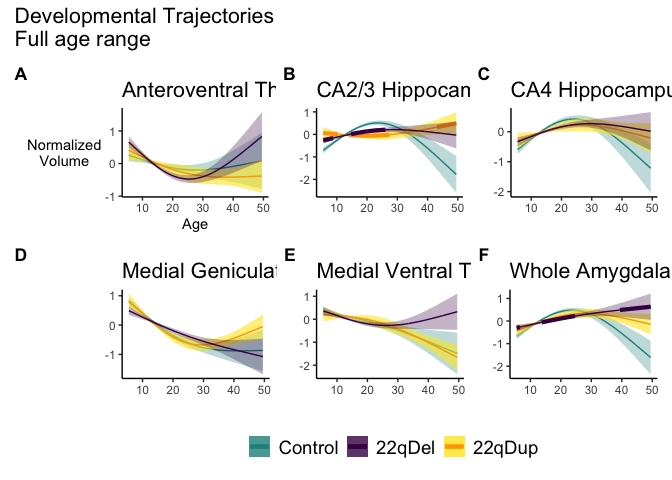
\includegraphics{22q_subcort_volumes_revised_files/figure-latex/unnamed-chunk-38-1.pdf}

\begin{Shaded}
\begin{Highlighting}[]
\CommentTok{\#ggsave(plot=plot\_age\_gd, filename=file.path(project,"figures/age/age\_gamms\_curves\_gdiff\_full.pdf"), width=12, height=7, device = "pdf")}
\CommentTok{\#ggsave(plot=plot\_age\_gd, filename=file.path(project,"figures/age/age\_gamms\_curves\_gdiff\_full.png"), width=12, height=7, device = "png", dpi = 300)}
\end{Highlighting}
\end{Shaded}

check some additional ones

\begin{Shaded}
\begin{Highlighting}[]
\FunctionTok{lapply}\NormalTok{(all\_names\_normed, }\ControlFlowTok{function}\NormalTok{(n) }\FunctionTok{plot\_gamm\_gdiff}\NormalTok{(}\AttributeTok{list=}\NormalTok{mat\_full\_gdiff, }\AttributeTok{name=}\NormalTok{n,}\AttributeTok{xlab=}\StringTok{"Age"}\NormalTok{,}\AttributeTok{ylab=}\StringTok{"Normalized}\SpecialCharTok{\textbackslash{}n}\StringTok{Volume"}\NormalTok{, }\AttributeTok{title=}\NormalTok{n))}
\end{Highlighting}
\end{Shaded}

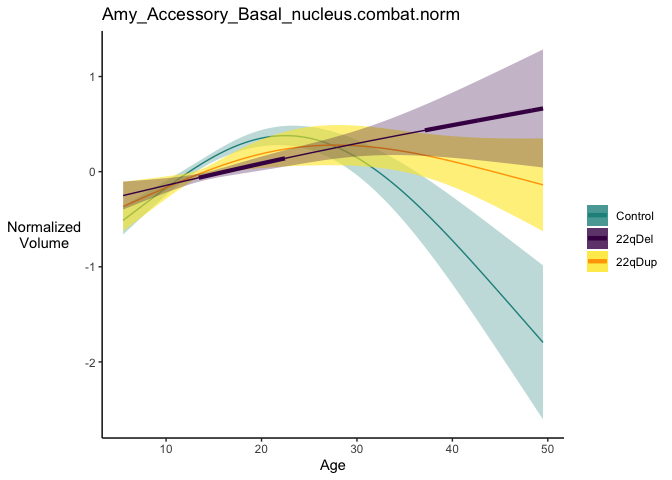
\includegraphics{22q_subcort_volumes_revised_files/figure-latex/unnamed-chunk-39-1.pdf}
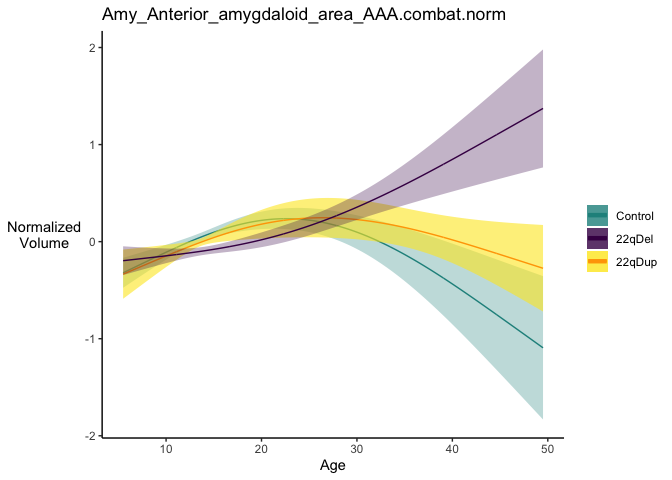
\includegraphics{22q_subcort_volumes_revised_files/figure-latex/unnamed-chunk-39-2.pdf}
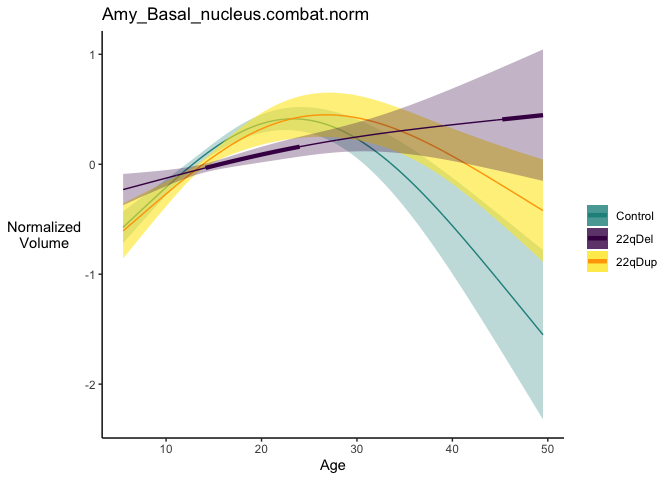
\includegraphics{22q_subcort_volumes_revised_files/figure-latex/unnamed-chunk-39-3.pdf}
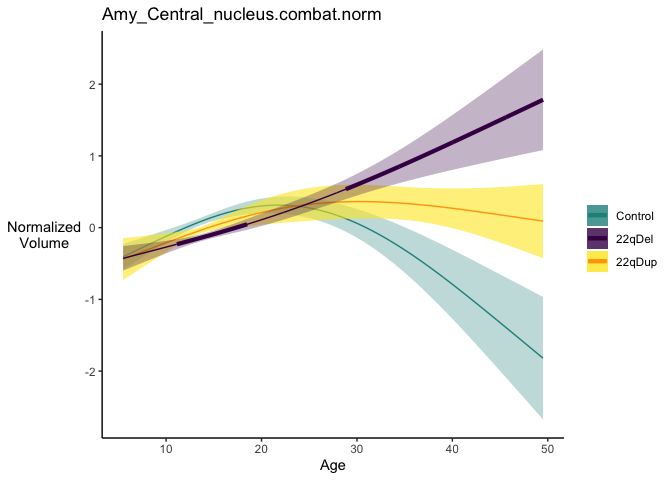
\includegraphics{22q_subcort_volumes_revised_files/figure-latex/unnamed-chunk-39-4.pdf}
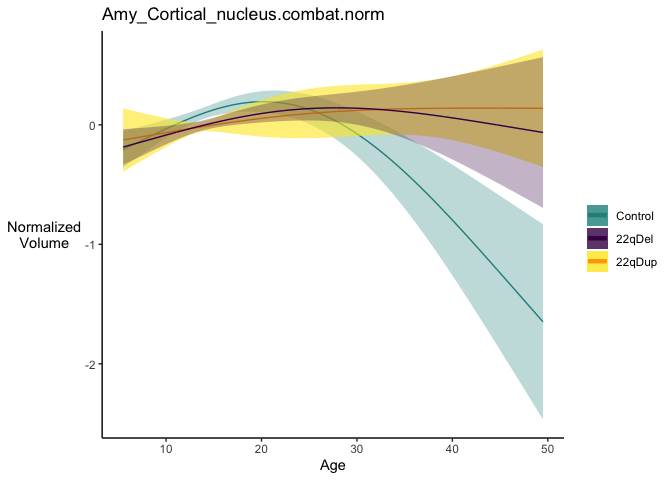
\includegraphics{22q_subcort_volumes_revised_files/figure-latex/unnamed-chunk-39-5.pdf}
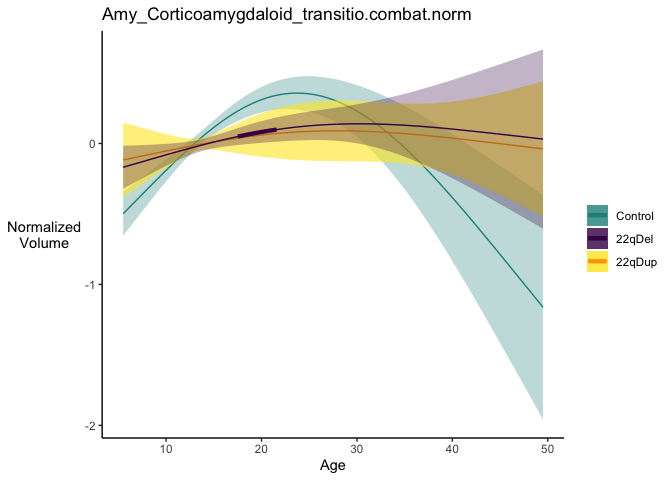
\includegraphics{22q_subcort_volumes_revised_files/figure-latex/unnamed-chunk-39-6.pdf}
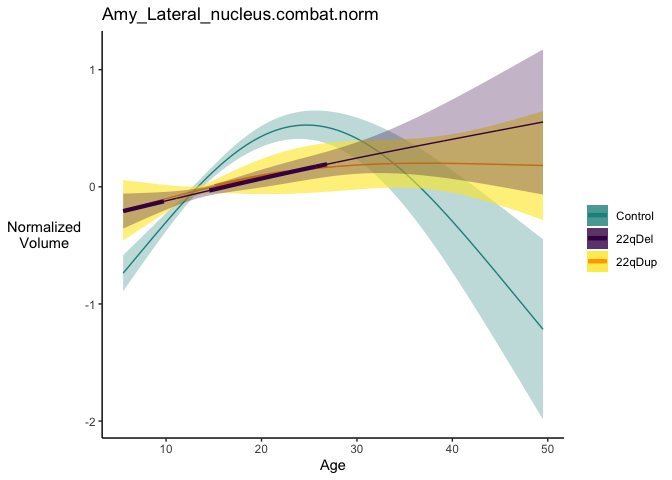
\includegraphics{22q_subcort_volumes_revised_files/figure-latex/unnamed-chunk-39-7.pdf}
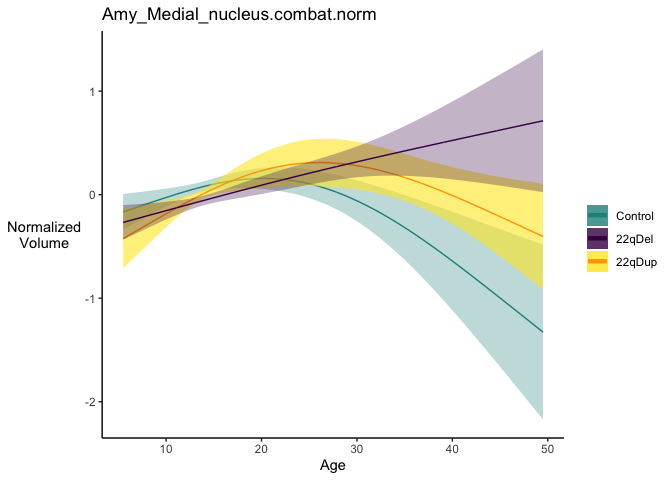
\includegraphics{22q_subcort_volumes_revised_files/figure-latex/unnamed-chunk-39-8.pdf}
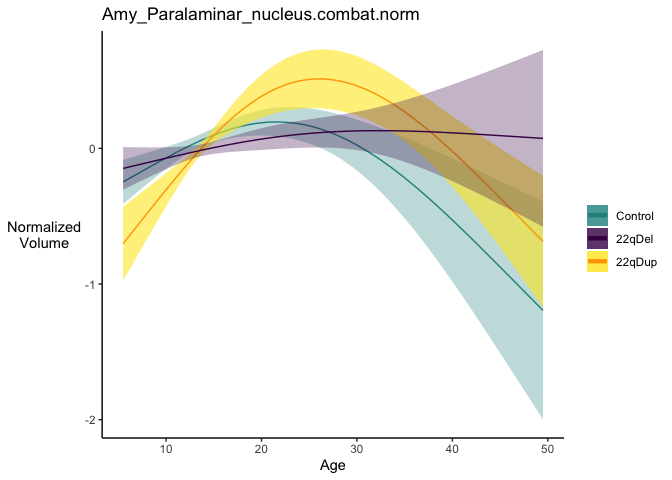
\includegraphics{22q_subcort_volumes_revised_files/figure-latex/unnamed-chunk-39-9.pdf}
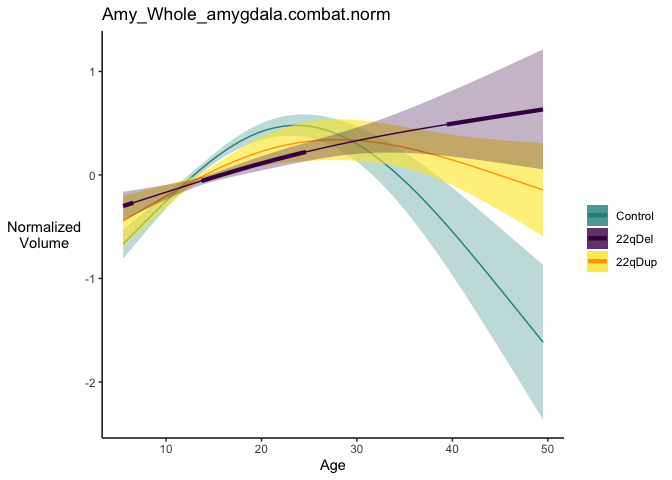
\includegraphics{22q_subcort_volumes_revised_files/figure-latex/unnamed-chunk-39-10.pdf}
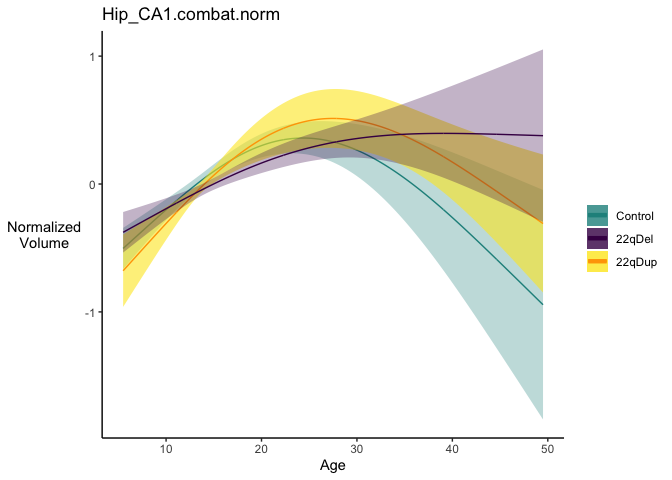
\includegraphics{22q_subcort_volumes_revised_files/figure-latex/unnamed-chunk-39-11.pdf}
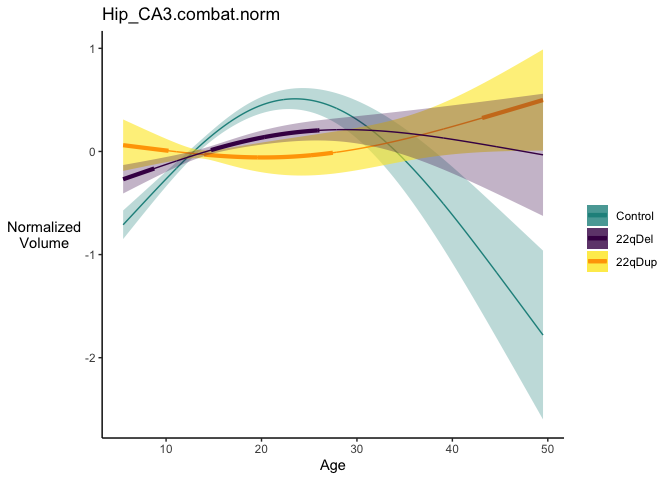
\includegraphics{22q_subcort_volumes_revised_files/figure-latex/unnamed-chunk-39-12.pdf}
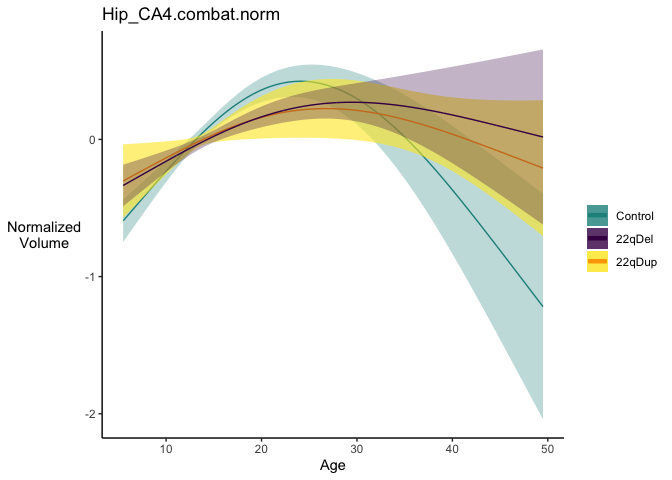
\includegraphics{22q_subcort_volumes_revised_files/figure-latex/unnamed-chunk-39-13.pdf}
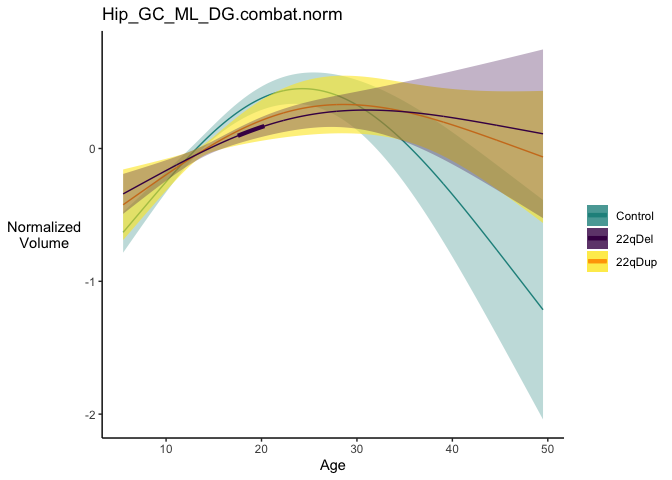
\includegraphics{22q_subcort_volumes_revised_files/figure-latex/unnamed-chunk-39-14.pdf}
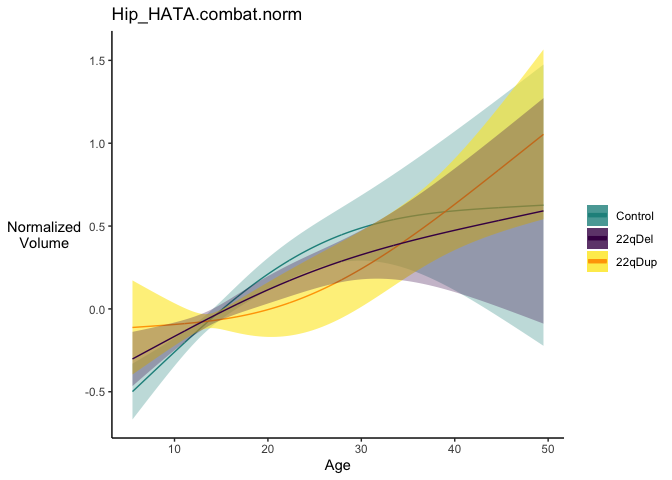
\includegraphics{22q_subcort_volumes_revised_files/figure-latex/unnamed-chunk-39-15.pdf}
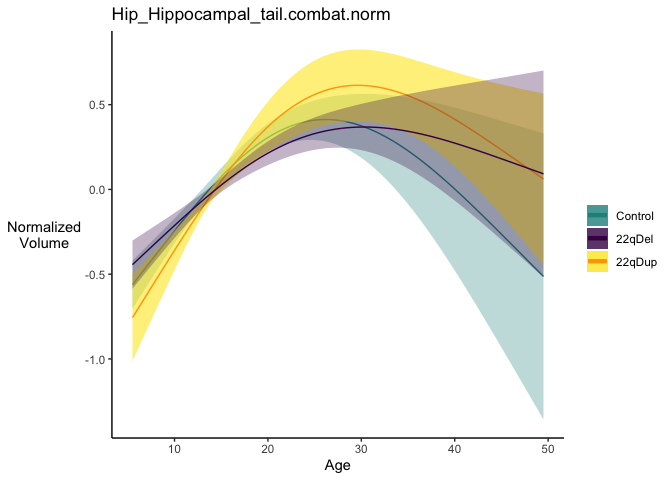
\includegraphics{22q_subcort_volumes_revised_files/figure-latex/unnamed-chunk-39-16.pdf}
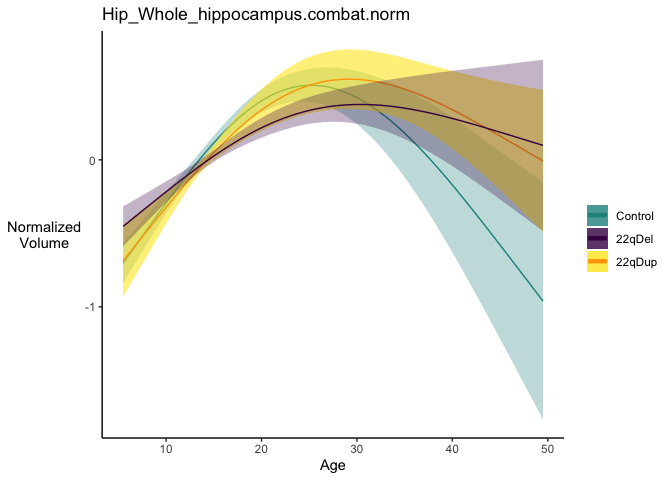
\includegraphics{22q_subcort_volumes_revised_files/figure-latex/unnamed-chunk-39-17.pdf}
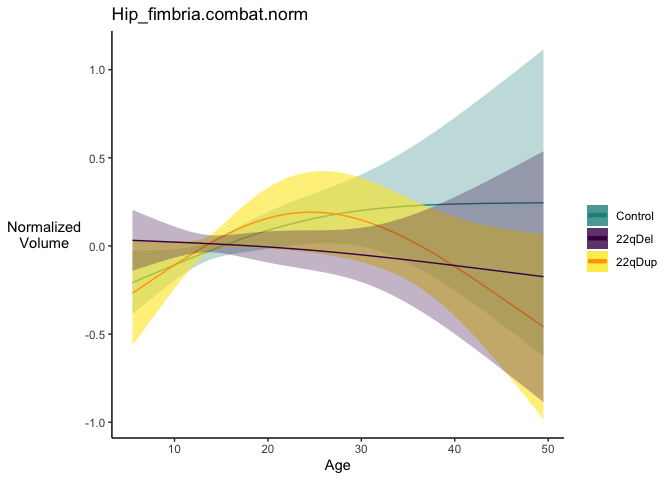
\includegraphics{22q_subcort_volumes_revised_files/figure-latex/unnamed-chunk-39-18.pdf}
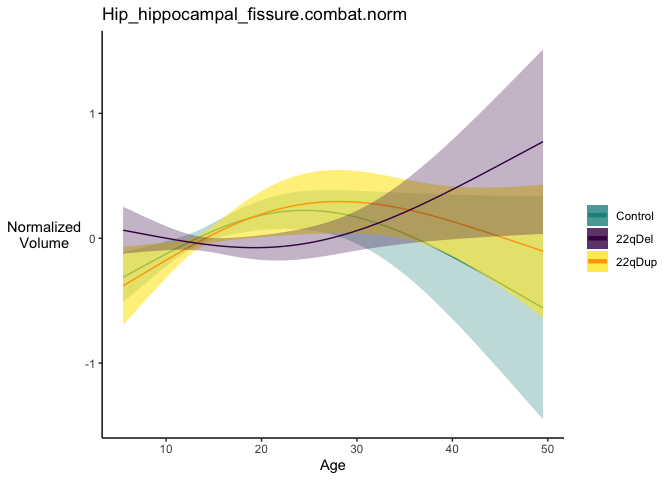
\includegraphics{22q_subcort_volumes_revised_files/figure-latex/unnamed-chunk-39-19.pdf}
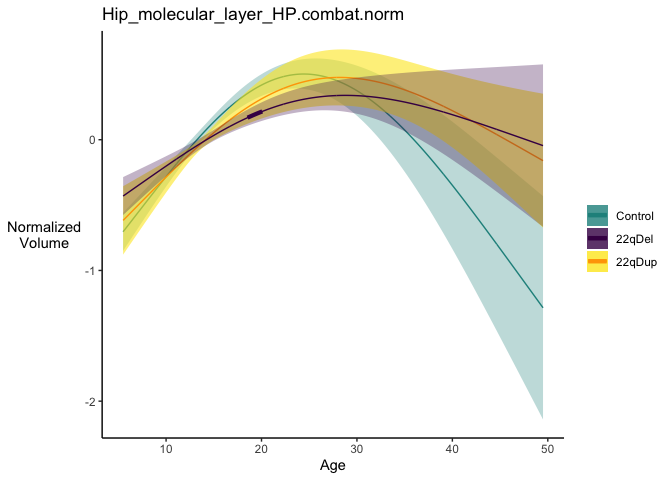
\includegraphics{22q_subcort_volumes_revised_files/figure-latex/unnamed-chunk-39-20.pdf}
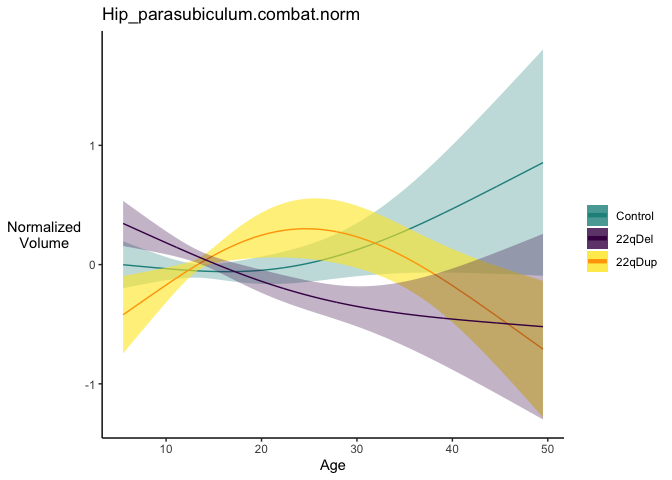
\includegraphics{22q_subcort_volumes_revised_files/figure-latex/unnamed-chunk-39-21.pdf}
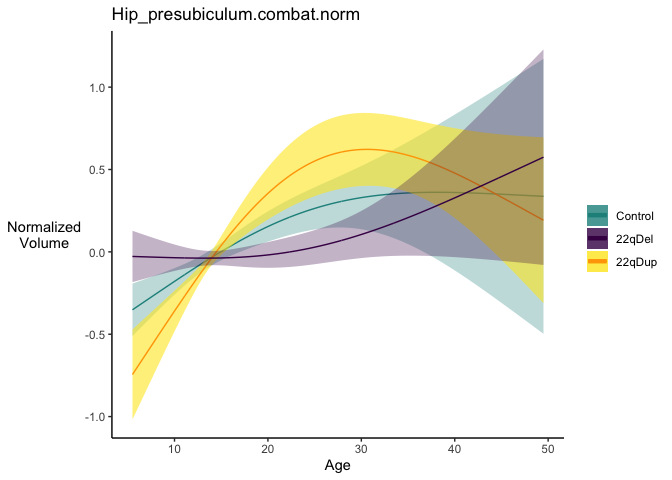
\includegraphics{22q_subcort_volumes_revised_files/figure-latex/unnamed-chunk-39-22.pdf}
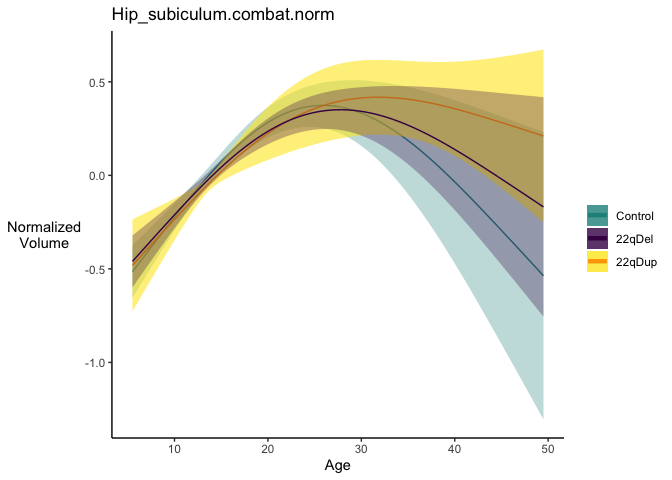
\includegraphics{22q_subcort_volumes_revised_files/figure-latex/unnamed-chunk-39-23.pdf}
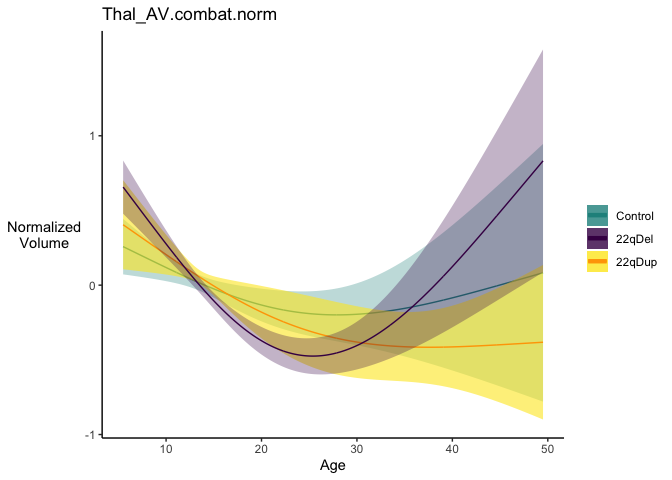
\includegraphics{22q_subcort_volumes_revised_files/figure-latex/unnamed-chunk-39-24.pdf}
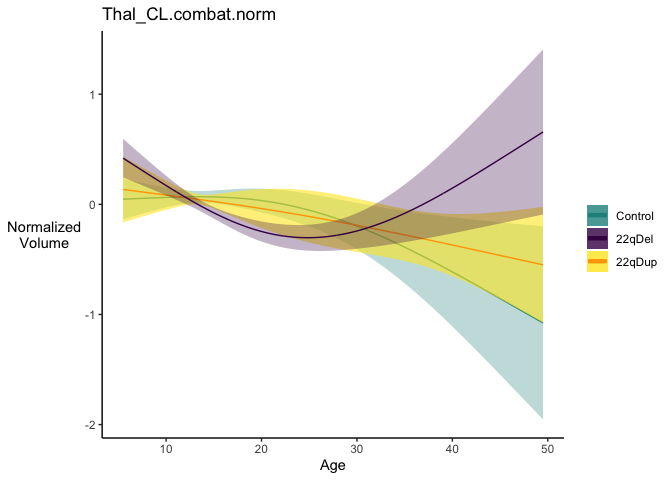
\includegraphics{22q_subcort_volumes_revised_files/figure-latex/unnamed-chunk-39-25.pdf}
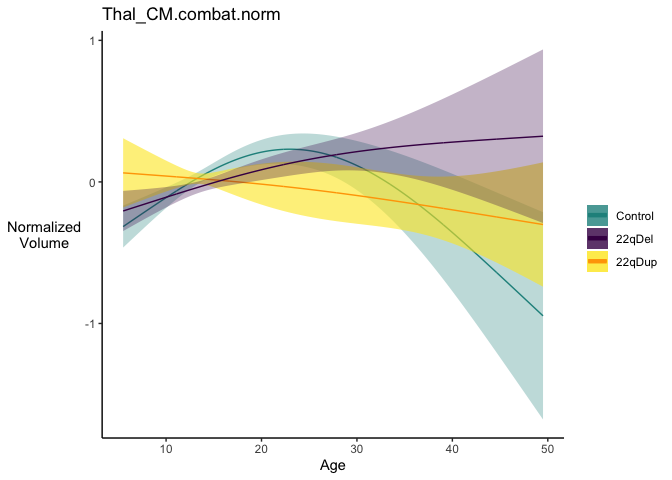
\includegraphics{22q_subcort_volumes_revised_files/figure-latex/unnamed-chunk-39-26.pdf}
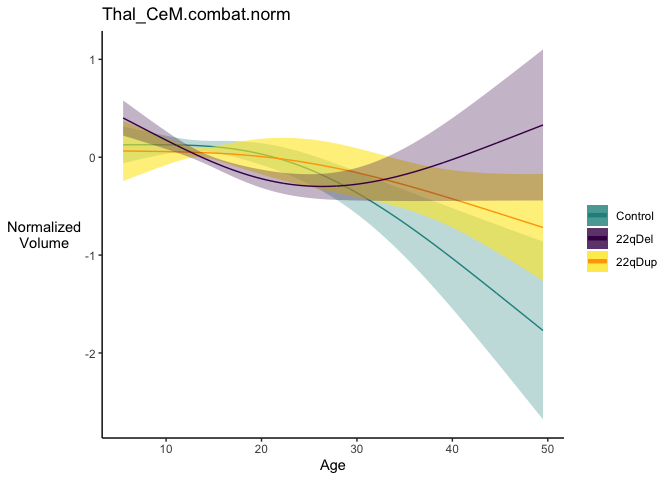
\includegraphics{22q_subcort_volumes_revised_files/figure-latex/unnamed-chunk-39-27.pdf}
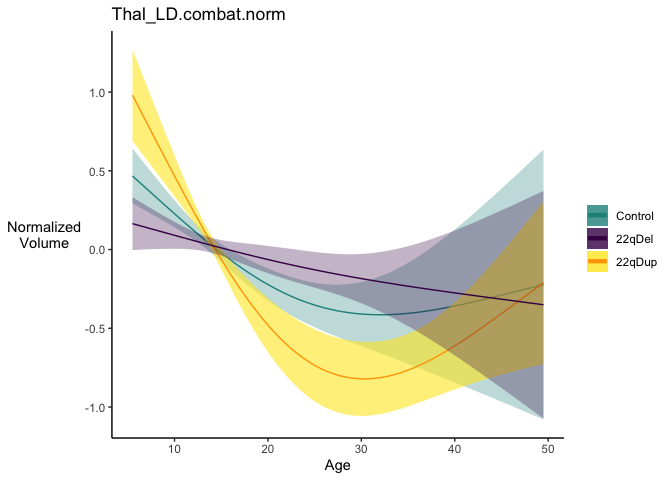
\includegraphics{22q_subcort_volumes_revised_files/figure-latex/unnamed-chunk-39-28.pdf}
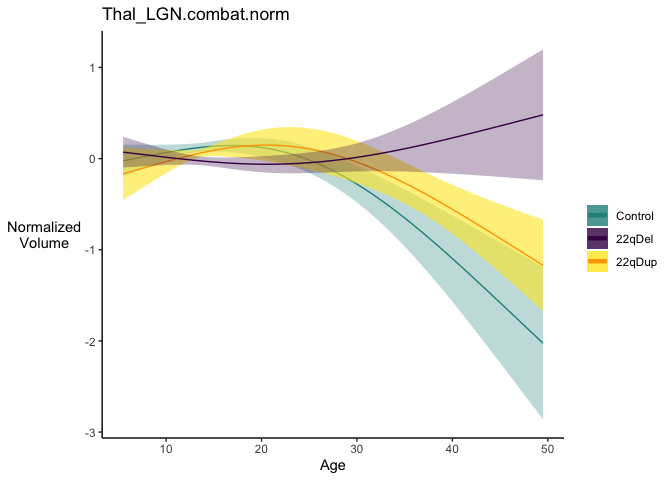
\includegraphics{22q_subcort_volumes_revised_files/figure-latex/unnamed-chunk-39-29.pdf}
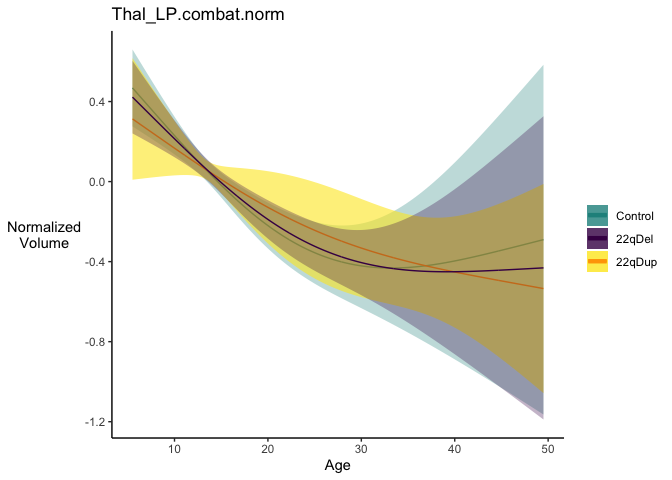
\includegraphics{22q_subcort_volumes_revised_files/figure-latex/unnamed-chunk-39-30.pdf}
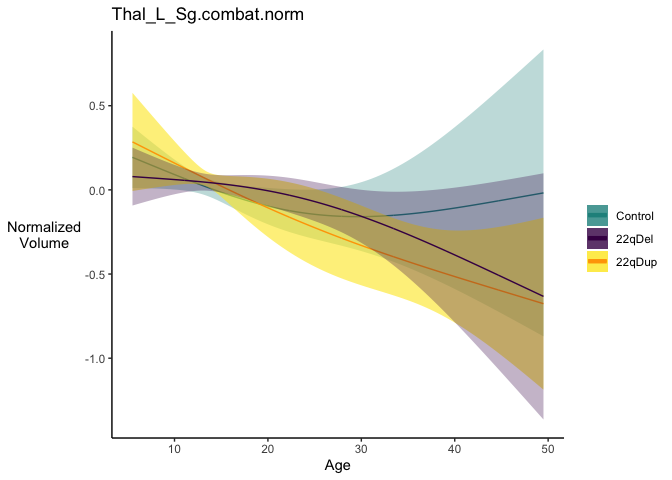
\includegraphics{22q_subcort_volumes_revised_files/figure-latex/unnamed-chunk-39-31.pdf}
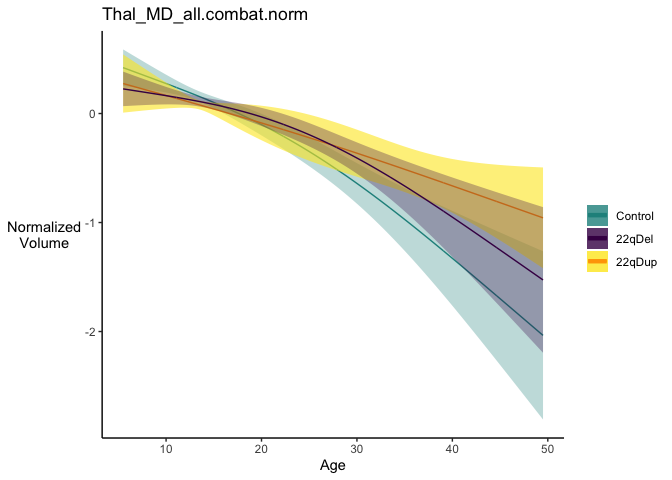
\includegraphics{22q_subcort_volumes_revised_files/figure-latex/unnamed-chunk-39-32.pdf}
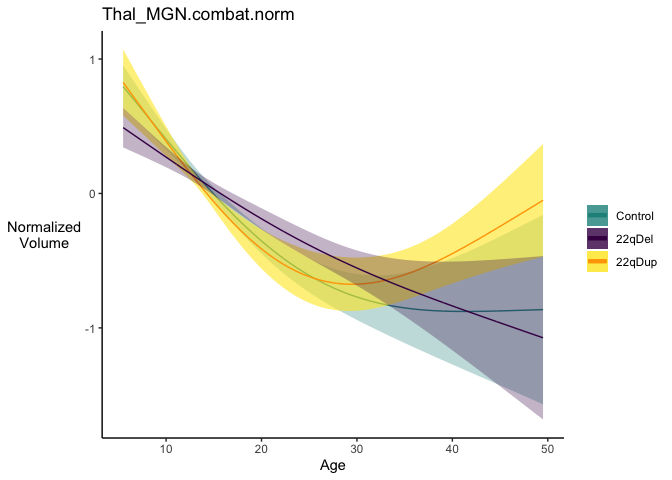
\includegraphics{22q_subcort_volumes_revised_files/figure-latex/unnamed-chunk-39-33.pdf}
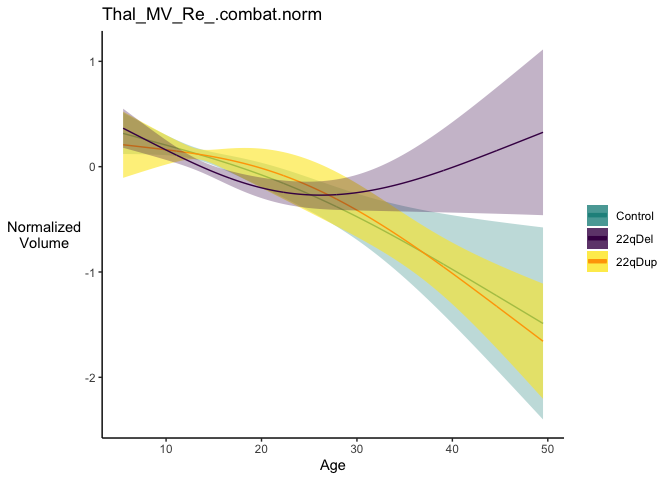
\includegraphics{22q_subcort_volumes_revised_files/figure-latex/unnamed-chunk-39-34.pdf}
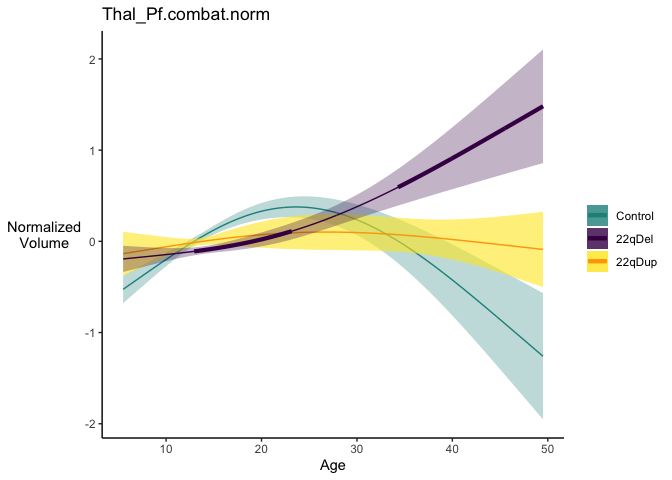
\includegraphics{22q_subcort_volumes_revised_files/figure-latex/unnamed-chunk-39-35.pdf}
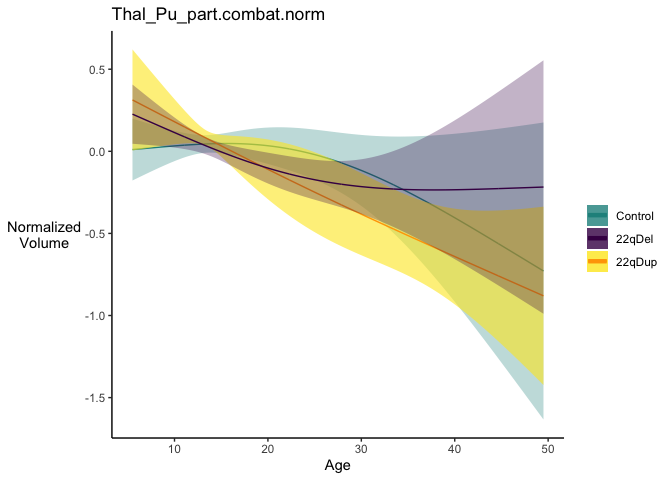
\includegraphics{22q_subcort_volumes_revised_files/figure-latex/unnamed-chunk-39-36.pdf}
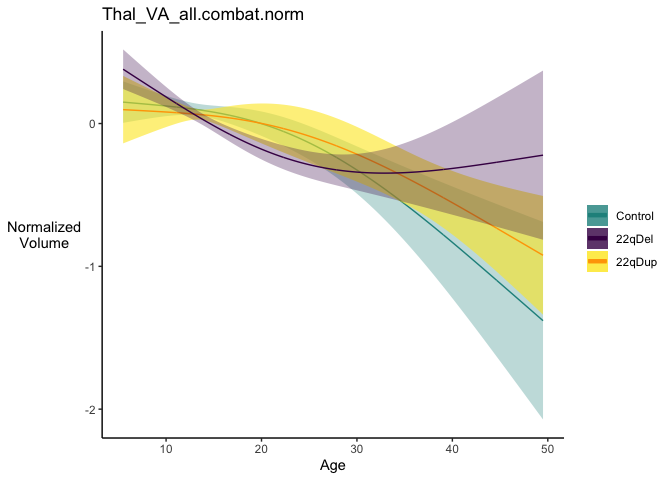
\includegraphics{22q_subcort_volumes_revised_files/figure-latex/unnamed-chunk-39-37.pdf}
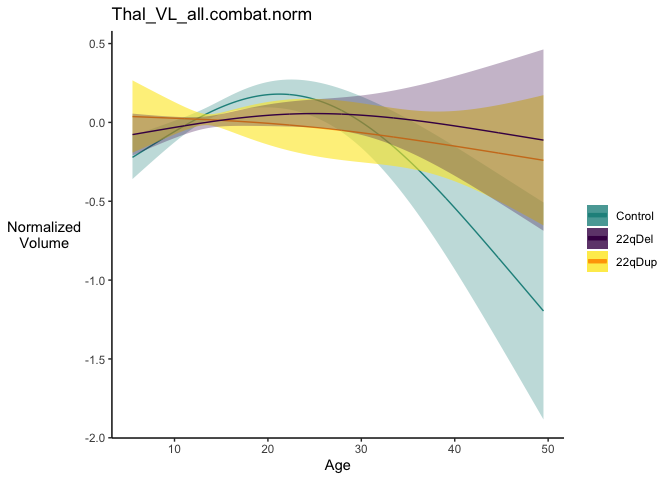
\includegraphics{22q_subcort_volumes_revised_files/figure-latex/unnamed-chunk-39-38.pdf}
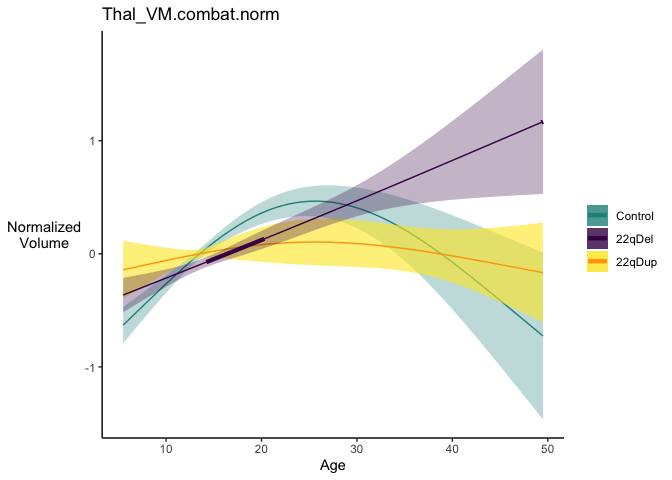
\includegraphics{22q_subcort_volumes_revised_files/figure-latex/unnamed-chunk-39-39.pdf}
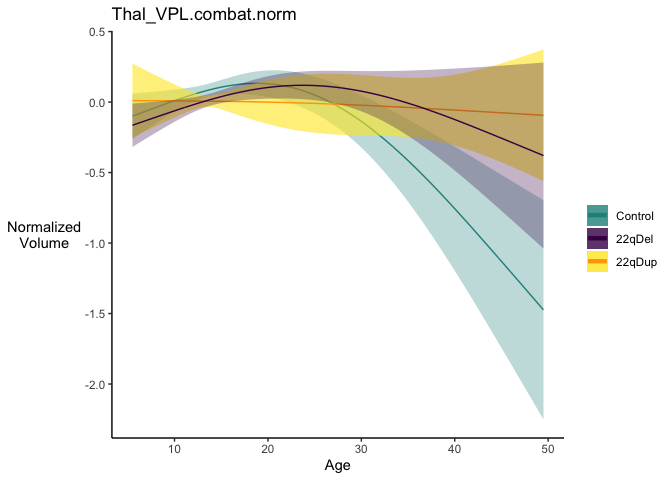
\includegraphics{22q_subcort_volumes_revised_files/figure-latex/unnamed-chunk-39-40.pdf}
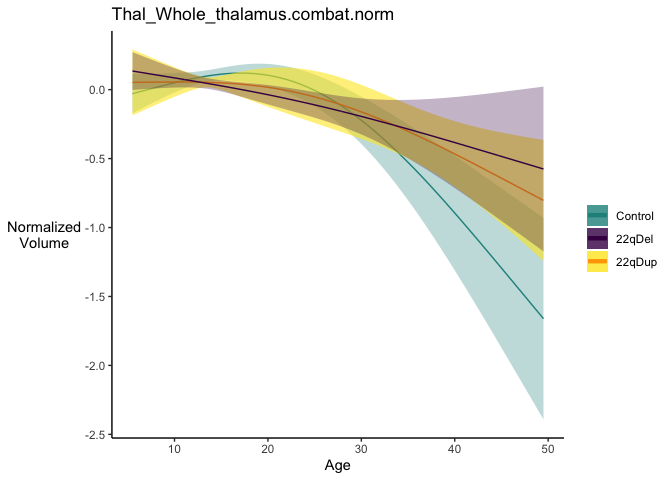
\includegraphics{22q_subcort_volumes_revised_files/figure-latex/unnamed-chunk-39-41.pdf}
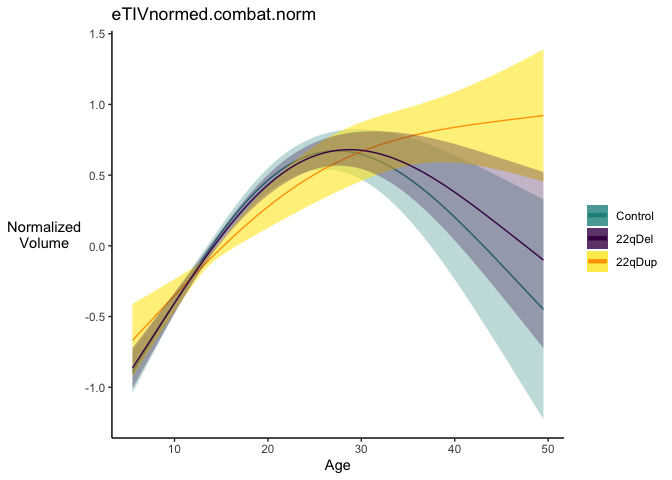
\includegraphics{22q_subcort_volumes_revised_files/figure-latex/unnamed-chunk-39-42.pdf}

plot age gamms for young sample

\begin{Shaded}
\begin{Highlighting}[]
\CommentTok{\#plot chosen gamms}
\NormalTok{thal\_av\_young }\OtherTok{\textless{}{-}} \FunctionTok{plot\_gamm\_resid}\NormalTok{(}\AttributeTok{list=}\NormalTok{maturation\_young, }\AttributeTok{name=}\StringTok{"Thal\_AV.combat.norm"}\NormalTok{,}\AttributeTok{xlab=}\StringTok{"Age"}\NormalTok{,}\AttributeTok{ylab=}\StringTok{"Normalized}\SpecialCharTok{\textbackslash{}n}\StringTok{Volume"}\NormalTok{, }\AttributeTok{title=}\StringTok{"Anteroventral Thalamus"}\NormalTok{)}
\NormalTok{hip\_ca3\_young }\OtherTok{\textless{}{-}} \FunctionTok{plot\_gamm\_resid}\NormalTok{(}\AttributeTok{list=}\NormalTok{maturation\_young, }\AttributeTok{name=}\StringTok{"Hip\_CA3.combat.norm"}\NormalTok{,}\AttributeTok{xlab=}\StringTok{""}\NormalTok{,}\AttributeTok{ylab=}\StringTok{""}\NormalTok{, }\AttributeTok{title=}\StringTok{"CA2/3 Hippocampus"}\NormalTok{)}
\NormalTok{amy\_whole\_young }\OtherTok{\textless{}{-}} \FunctionTok{plot\_gamm\_resid}\NormalTok{(}\AttributeTok{list=}\NormalTok{maturation\_young, }\AttributeTok{name=}\StringTok{"Amy\_Whole\_amygdala.combat.norm"}\NormalTok{,}\AttributeTok{xlab=}\StringTok{""}\NormalTok{,}\AttributeTok{ylab=}\StringTok{""}\NormalTok{, }\AttributeTok{title=}\StringTok{"Whole Amygdala"}\NormalTok{)}
\NormalTok{thal\_mgn\_young }\OtherTok{\textless{}{-}} \FunctionTok{plot\_gamm\_resid}\NormalTok{(}\AttributeTok{list=}\NormalTok{maturation\_young, }\AttributeTok{name=}\StringTok{"Thal\_MGN.combat.norm"}\NormalTok{,}\AttributeTok{xlab=}\StringTok{""}\NormalTok{,}\AttributeTok{ylab=}\StringTok{""}\NormalTok{, }\AttributeTok{title=}\StringTok{"Medial Geniculate Thalamus"}\NormalTok{)}
\NormalTok{thal\_mvre\_young }\OtherTok{\textless{}{-}} \FunctionTok{plot\_gamm\_resid}\NormalTok{(}\AttributeTok{list=}\NormalTok{maturation\_young, }\AttributeTok{name=}\StringTok{"Thal\_MV\_Re\_.combat.norm"}\NormalTok{,}\AttributeTok{xlab=}\StringTok{""}\NormalTok{,}\AttributeTok{ylab=}\StringTok{""}\NormalTok{, }\AttributeTok{title=}\StringTok{"Medial Ventral Thalamus"}\NormalTok{)}
\NormalTok{hip\_ca4\_young }\OtherTok{\textless{}{-}} \FunctionTok{plot\_gamm\_resid}\NormalTok{(}\AttributeTok{list=}\NormalTok{maturation\_young, }\AttributeTok{name=}\StringTok{"Hip\_CA4.combat.norm"}\NormalTok{,}\AttributeTok{xlab=}\StringTok{""}\NormalTok{,}\AttributeTok{ylab=}\StringTok{""}\NormalTok{, }\AttributeTok{title=}\StringTok{"CA4 Hippocampus"}\NormalTok{)}

\NormalTok{plot\_age\_young }\OtherTok{\textless{}{-}}\NormalTok{ (thal\_av\_young }\SpecialCharTok{+}\NormalTok{ hip\_ca3\_young }\SpecialCharTok{+}\NormalTok{ hip\_ca4\_young) }\SpecialCharTok{/}\NormalTok{ (thal\_mgn\_young }\SpecialCharTok{+}\NormalTok{ thal\_mvre\_young }\SpecialCharTok{+}\NormalTok{ amy\_whole\_young) }\SpecialCharTok{+} \FunctionTok{plot\_layout}\NormalTok{(}\AttributeTok{guides =} \StringTok{"collect"}\NormalTok{) }\SpecialCharTok{+} \FunctionTok{plot\_annotation}\NormalTok{(}\AttributeTok{tag\_levels =} \StringTok{\textquotesingle{}A\textquotesingle{}}\NormalTok{, }\AttributeTok{title=}\StringTok{"Developmental Trajectories}\SpecialCharTok{\textbackslash{}n}\StringTok{Age \textless{} 35"}\NormalTok{) }\SpecialCharTok{\&}   \FunctionTok{theme}\NormalTok{(}\AttributeTok{plot.tag =} \FunctionTok{element\_text}\NormalTok{(}\AttributeTok{face =} \StringTok{\textquotesingle{}bold\textquotesingle{}}\NormalTok{)) }\SpecialCharTok{+} \FunctionTok{theme}\NormalTok{(}\AttributeTok{legend.position =} \StringTok{"bottom"}\NormalTok{, }\AttributeTok{legend.text=}\FunctionTok{element\_text}\NormalTok{(}\AttributeTok{size=}\DecValTok{14}\NormalTok{), }\AttributeTok{plot.title =} \FunctionTok{element\_text}\NormalTok{(}\AttributeTok{size=}\DecValTok{16}\NormalTok{, }\AttributeTok{hjust =} \DecValTok{0}\NormalTok{)) }

\NormalTok{plot\_age\_young}
\end{Highlighting}
\end{Shaded}

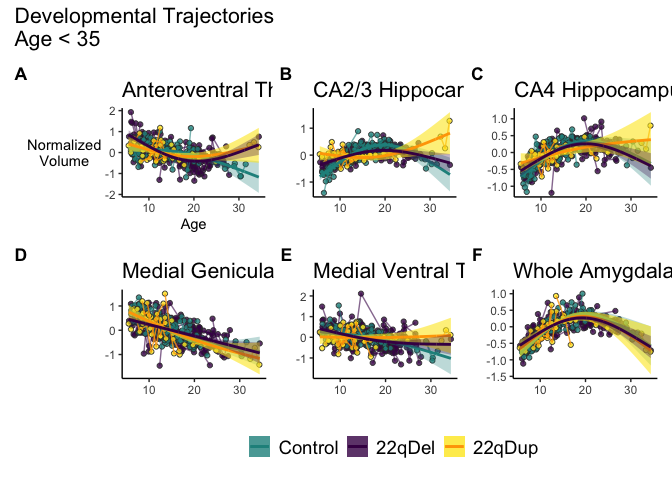
\includegraphics{22q_subcort_volumes_revised_files/figure-latex/unnamed-chunk-40-1.pdf}

\begin{Shaded}
\begin{Highlighting}[]
\CommentTok{\#ggsave(plot=plot\_age\_young, filename=file.path(project,"figures/age/age\_gamms\_curves\_resid\_u35.pdf"), width=12, height=7, device = "pdf")}
\CommentTok{\#ggsave(plot=plot\_age\_young, filename=file.path(project,"figures/age/age\_gamms\_curves\_resid\_u35.png"), width=12, height=7, device = "png", dpi = 300)}
\end{Highlighting}
\end{Shaded}

plot age gamms with group differences for young sample

\begin{Shaded}
\begin{Highlighting}[]
\CommentTok{\#plot chosen gamms}
\NormalTok{thal\_av\_young\_gd }\OtherTok{\textless{}{-}} \FunctionTok{plot\_gamm\_gdiff}\NormalTok{(}\AttributeTok{list=}\NormalTok{mat\_young\_gdiff, }\AttributeTok{name=}\StringTok{"Thal\_AV.combat.norm"}\NormalTok{,}\AttributeTok{xlab=}\StringTok{"Age"}\NormalTok{,}\AttributeTok{ylab=}\StringTok{"Normalized}\SpecialCharTok{\textbackslash{}n}\StringTok{Volume"}\NormalTok{, }\AttributeTok{title=}\StringTok{"Anteroventral Thalamus"}\NormalTok{)}
\NormalTok{hip\_ca3\_young\_gd }\OtherTok{\textless{}{-}} \FunctionTok{plot\_gamm\_gdiff}\NormalTok{(}\AttributeTok{list=}\NormalTok{mat\_young\_gdiff, }\AttributeTok{name=}\StringTok{"Hip\_CA3.combat.norm"}\NormalTok{,}\AttributeTok{xlab=}\StringTok{""}\NormalTok{,}\AttributeTok{ylab=}\StringTok{""}\NormalTok{, }\AttributeTok{title=}\StringTok{"CA2/3 Hippocampus"}\NormalTok{)}
\NormalTok{amy\_whole\_young\_gd }\OtherTok{\textless{}{-}} \FunctionTok{plot\_gamm\_gdiff}\NormalTok{(}\AttributeTok{list=}\NormalTok{mat\_young\_gdiff, }\AttributeTok{name=}\StringTok{"Amy\_Whole\_amygdala.combat.norm"}\NormalTok{,}\AttributeTok{xlab=}\StringTok{""}\NormalTok{,}\AttributeTok{ylab=}\StringTok{""}\NormalTok{, }\AttributeTok{title=}\StringTok{"Whole Amygdala"}\NormalTok{)}
\NormalTok{thal\_mgn\_young\_gd }\OtherTok{\textless{}{-}} \FunctionTok{plot\_gamm\_gdiff}\NormalTok{(}\AttributeTok{list=}\NormalTok{mat\_young\_gdiff, }\AttributeTok{name=}\StringTok{"Thal\_MGN.combat.norm"}\NormalTok{,}\AttributeTok{xlab=}\StringTok{""}\NormalTok{,}\AttributeTok{ylab=}\StringTok{""}\NormalTok{, }\AttributeTok{title=}\StringTok{"Medial Geniculate Thalamus"}\NormalTok{)}
\NormalTok{thal\_mvre\_young\_gd }\OtherTok{\textless{}{-}} \FunctionTok{plot\_gamm\_gdiff}\NormalTok{(}\AttributeTok{list=}\NormalTok{mat\_young\_gdiff, }\AttributeTok{name=}\StringTok{"Thal\_MV\_Re\_.combat.norm"}\NormalTok{,}\AttributeTok{xlab=}\StringTok{""}\NormalTok{,}\AttributeTok{ylab=}\StringTok{""}\NormalTok{, }\AttributeTok{title=}\StringTok{"Medial Ventral Thalamus"}\NormalTok{)}
\NormalTok{hip\_ca4\_young\_gd }\OtherTok{\textless{}{-}} \FunctionTok{plot\_gamm\_gdiff}\NormalTok{(}\AttributeTok{list=}\NormalTok{mat\_young\_gdiff, }\AttributeTok{name=}\StringTok{"Hip\_CA4.combat.norm"}\NormalTok{,}\AttributeTok{xlab=}\StringTok{""}\NormalTok{,}\AttributeTok{ylab=}\StringTok{""}\NormalTok{, }\AttributeTok{title=}\StringTok{"CA4 Hippocampus"}\NormalTok{)}

\NormalTok{plot\_age\_young\_gd }\OtherTok{\textless{}{-}}\NormalTok{ (thal\_av\_young\_gd }\SpecialCharTok{+}\NormalTok{ hip\_ca3\_young\_gd }\SpecialCharTok{+}\NormalTok{ hip\_ca4\_young\_gd) }\SpecialCharTok{/}\NormalTok{ (thal\_mgn\_young\_gd }\SpecialCharTok{+}\NormalTok{ thal\_mvre\_young\_gd }\SpecialCharTok{+}\NormalTok{ amy\_whole\_young\_gd) }\SpecialCharTok{+} \FunctionTok{plot\_layout}\NormalTok{(}\AttributeTok{guides =} \StringTok{"collect"}\NormalTok{) }\SpecialCharTok{+} \FunctionTok{plot\_annotation}\NormalTok{(}\AttributeTok{tag\_levels =} \StringTok{\textquotesingle{}A\textquotesingle{}}\NormalTok{, }\AttributeTok{title=}\StringTok{"Developmental Trajectories}\SpecialCharTok{\textbackslash{}n}\StringTok{Age \textless{} 35"}\NormalTok{) }\SpecialCharTok{\&}   \FunctionTok{theme}\NormalTok{(}\AttributeTok{plot.tag =} \FunctionTok{element\_text}\NormalTok{(}\AttributeTok{face =} \StringTok{\textquotesingle{}bold\textquotesingle{}}\NormalTok{)) }\SpecialCharTok{+} \FunctionTok{theme}\NormalTok{(}\AttributeTok{legend.position =} \StringTok{"bottom"}\NormalTok{, }\AttributeTok{legend.text=}\FunctionTok{element\_text}\NormalTok{(}\AttributeTok{size=}\DecValTok{14}\NormalTok{), }\AttributeTok{plot.title =} \FunctionTok{element\_text}\NormalTok{(}\AttributeTok{size=}\DecValTok{16}\NormalTok{, }\AttributeTok{hjust =} \DecValTok{0}\NormalTok{)) }

\NormalTok{plot\_age\_young\_gd}
\end{Highlighting}
\end{Shaded}

\includegraphics{22q_subcort_volumes_revised_files/figure-latex/unnamed-chunk-41-1.pdf}

\begin{Shaded}
\begin{Highlighting}[]
\CommentTok{\#ggsave(plot=plot\_age\_young\_gd, filename=file.path(project,"figures/age/age\_gamms\_curves\_gdiff\_u35.pdf"), width=12, height=7, device = "pdf")}
\CommentTok{\#ggsave(plot=plot\_age\_young\_gd, filename=file.path(project,"figures/age/age\_gamms\_curves\_gdiff\_u35.png"), width=12, height=7, device = "png", dpi = 300)}
\end{Highlighting}
\end{Shaded}

\hypertarget{supplemental}{%
\subsection{supplemental}\label{supplemental}}

export table of roi sizes

\begin{Shaded}
\begin{Highlighting}[]
\CommentTok{\# get average roi per group}
\NormalTok{group\_mean\_vols }\OtherTok{\textless{}{-}} \FunctionTok{data.frame}\NormalTok{(}\AttributeTok{Region=}\NormalTok{sc\_names)}
\ControlFlowTok{for}\NormalTok{(c }\ControlFlowTok{in}\NormalTok{ sc\_names)\{}
\NormalTok{  group\_mean\_vols[}\FunctionTok{which}\NormalTok{(group\_mean\_vols}\SpecialCharTok{$}\NormalTok{Region }\SpecialCharTok{==}\NormalTok{ c),}\StringTok{"22qDel"}\NormalTok{] }\OtherTok{\textless{}{-}} \FunctionTok{mean}\NormalTok{(}\FunctionTok{filter}\NormalTok{(demo\_sc, SUBJECT\_IDENTITY}\SpecialCharTok{==}\StringTok{"PATIENT{-}DEL"}\NormalTok{)[,c],}\AttributeTok{na.rm =} \ConstantTok{TRUE}\NormalTok{) }\SpecialCharTok{\%\textgreater{}\%} \FunctionTok{round}\NormalTok{(., }\AttributeTok{digits=}\DecValTok{0}\NormalTok{)}
\NormalTok{  group\_mean\_vols[}\FunctionTok{which}\NormalTok{(group\_mean\_vols}\SpecialCharTok{$}\NormalTok{Region }\SpecialCharTok{==}\NormalTok{ c),}\StringTok{"TD"}\NormalTok{] }\OtherTok{\textless{}{-}} \FunctionTok{mean}\NormalTok{(}\FunctionTok{filter}\NormalTok{(demo\_sc, SUBJECT\_IDENTITY}\SpecialCharTok{==}\StringTok{"CONTROL"}\NormalTok{)[,c],}\AttributeTok{na.rm =} \ConstantTok{TRUE}\NormalTok{) }\SpecialCharTok{\%\textgreater{}\%} \FunctionTok{round}\NormalTok{(., }\AttributeTok{digits=}\DecValTok{0}\NormalTok{)}
\NormalTok{  group\_mean\_vols[}\FunctionTok{which}\NormalTok{(group\_mean\_vols}\SpecialCharTok{$}\NormalTok{Region }\SpecialCharTok{==}\NormalTok{ c),}\StringTok{"22qDup"}\NormalTok{] }\OtherTok{\textless{}{-}} \FunctionTok{mean}\NormalTok{(}\FunctionTok{filter}\NormalTok{(demo\_sc, SUBJECT\_IDENTITY}\SpecialCharTok{==}\StringTok{"PATIENT{-}DUP"}\NormalTok{)[,c],}\AttributeTok{na.rm =} \ConstantTok{TRUE}\NormalTok{) }\SpecialCharTok{\%\textgreater{}\%} \FunctionTok{round}\NormalTok{(., }\AttributeTok{digits=}\DecValTok{0}\NormalTok{)}
\NormalTok{\}}
\NormalTok{group\_mean\_vols }\OtherTok{\textless{}{-}}\NormalTok{ group\_mean\_vols[}\FunctionTok{order}\NormalTok{(group\_mean\_vols}\SpecialCharTok{$}\NormalTok{TD),]}

\CommentTok{\# get region names for matching}
\NormalTok{group\_mean\_vols}\SpecialCharTok{$}\NormalTok{r }\OtherTok{\textless{}{-}} \FunctionTok{gsub}\NormalTok{(}\StringTok{"Thal\_"}\NormalTok{,}\StringTok{""}\NormalTok{,group\_mean\_vols}\SpecialCharTok{$}\NormalTok{Region)}
\NormalTok{group\_mean\_vols}\SpecialCharTok{$}\NormalTok{r }\OtherTok{\textless{}{-}} \FunctionTok{gsub}\NormalTok{(}\StringTok{"Amy\_"}\NormalTok{,}\StringTok{""}\NormalTok{,group\_mean\_vols}\SpecialCharTok{$}\NormalTok{r)}
\NormalTok{group\_mean\_vols}\SpecialCharTok{$}\NormalTok{r }\OtherTok{\textless{}{-}} \FunctionTok{gsub}\NormalTok{(}\StringTok{"Hip\_"}\NormalTok{,}\StringTok{""}\NormalTok{,group\_mean\_vols}\SpecialCharTok{$}\NormalTok{r)}

\CommentTok{\# merge with full names}
\CommentTok{\#save\_dosage\_effect \textless{}{-} merge(x=save\_dosage\_effect, y=lut[c("Structure","Name","region\_match")], by.x="Region",by.y="region\_match", all.x=TRUE)}
\NormalTok{group\_mean\_match }\OtherTok{\textless{}{-}} \FunctionTok{merge}\NormalTok{(}\AttributeTok{x=}\NormalTok{group\_mean\_vols, }\AttributeTok{y=}\NormalTok{lut\_unique[,}\FunctionTok{c}\NormalTok{(}\StringTok{"Structure"}\NormalTok{,}\StringTok{"bilat\_name"}\NormalTok{,}\StringTok{"bilat\_match"}\NormalTok{)], }\AttributeTok{by.x=}\StringTok{"r"}\NormalTok{,}\AttributeTok{by.y=}\StringTok{"bilat\_match"}\NormalTok{, }\AttributeTok{all.x=}\ConstantTok{TRUE}\NormalTok{)}

\CommentTok{\# select cols}
\NormalTok{group\_mean\_out }\OtherTok{\textless{}{-}}\NormalTok{ group\_mean\_match[}\FunctionTok{order}\NormalTok{(group\_mean\_match[,}\StringTok{"22qDel"}\NormalTok{]),}\FunctionTok{c}\NormalTok{(}\StringTok{"Structure"}\NormalTok{,}\StringTok{"bilat\_name"}\NormalTok{,}\StringTok{"22qDel"}\NormalTok{,}\StringTok{"TD"}\NormalTok{,}\StringTok{"22qDup"}\NormalTok{)] }\SpecialCharTok{\%\textgreater{}\%} \FunctionTok{rename}\NormalTok{(}\StringTok{"Region"}\OtherTok{=}\StringTok{"bilat\_name"}\NormalTok{)}

\NormalTok{group\_mean\_table }\OtherTok{\textless{}{-}}\NormalTok{ group\_mean\_out }\SpecialCharTok{\%\textgreater{}\%} \FunctionTok{gt}\NormalTok{() }\SpecialCharTok{\%\textgreater{}\%} 
  \FunctionTok{tab\_style}\NormalTok{(}\AttributeTok{style =} \FunctionTok{cell\_text}\NormalTok{(}\AttributeTok{weight =} \StringTok{"bold"}\NormalTok{),}\AttributeTok{locations =} \FunctionTok{list}\NormalTok{(}\FunctionTok{cells\_title}\NormalTok{(),}\FunctionTok{cells\_column\_labels}\NormalTok{())) }\SpecialCharTok{\%\textgreater{}\%}
  \FunctionTok{cols\_align}\NormalTok{(}\AttributeTok{align=}\StringTok{"right"}\NormalTok{, }\AttributeTok{columns=}\FunctionTok{everything}\NormalTok{()) }\SpecialCharTok{\%\textgreater{}\%} 
  \FunctionTok{tab\_header}\NormalTok{(}\StringTok{"Average volumes (mm\^{}3) by group"}\NormalTok{)}\SpecialCharTok{\%\textgreater{}\%}
  \FunctionTok{tab\_options}\NormalTok{(}\AttributeTok{data\_row.padding =} \FunctionTok{px}\NormalTok{(}\DecValTok{1}\NormalTok{)) }
\NormalTok{group\_mean\_table}
\CommentTok{\# gtsave(group\_mean\_table, filename = file.path(project,"figures/atlas/volumes.pdf"))}
\CommentTok{\# gtsave(group\_mean\_table, filename = file.path(project,"figures/atlas/volumes.png"))}
\CommentTok{\# gtsave(group\_mean\_table, filename = file.path(project,"figures/atlas/volumes.rtf"))}

\CommentTok{\# list in order for methods}
\NormalTok{group\_mean\_write }\OtherTok{\textless{}{-}}\NormalTok{ group\_mean\_out}
\FunctionTok{setorder}\NormalTok{(group\_mean\_write,Structure,Region)}
\end{Highlighting}
\end{Shaded}

To test for group differences, not just gene dosage effects (e.g.~del
\textless{} TD \& Dup \textless{} TD or Del \textless{} TD = Dup), use a
model with a binary variable for each group? or two separate
case/control models?

\begin{Shaded}
\begin{Highlighting}[]
\CommentTok{\#gamm\_combat \textless{}{-} lapply(sc\_names\_normed, function(r) gam(formula=reformulate( c("s(AGE,by=SUBJECT\_IDENTITY, bs=\textbackslash{}"tp\textbackslash{}", k=3, fx=TRUE)", "gene\_dosage", "SEX", "eTIVnormed", "site", "s(SUBJECTID, bs=\textbackslash{}"re\textbackslash{}", k=3)"), response=r), data=demo\_combat\_na\_gam, selection=TRUE, method="REML", na.action="na.omit"))}

\CommentTok{\# test random intercept model at each region separately in Del and Dup}
\NormalTok{gam\_combat\_del }\OtherTok{\textless{}{-}} \FunctionTok{lapply}\NormalTok{(sc\_names\_normed, }\ControlFlowTok{function}\NormalTok{(r) }\FunctionTok{gam}\NormalTok{(}\AttributeTok{formula=}\FunctionTok{reformulate}\NormalTok{( }\FunctionTok{c}\NormalTok{(}\StringTok{"s(AGE,by=SUBJECT\_IDENTITY, bs=}\SpecialCharTok{\textbackslash{}"}\StringTok{tp}\SpecialCharTok{\textbackslash{}"}\StringTok{, k=3, fx=TRUE)"}\NormalTok{, }\StringTok{"SUBJECT\_IDENTITY"}\NormalTok{, }\StringTok{"SEX"}\NormalTok{, }\StringTok{"eTIVnormed"}\NormalTok{, }\StringTok{"site"}\NormalTok{, }\StringTok{"s(SUBJECTID, bs=}\SpecialCharTok{\textbackslash{}"}\StringTok{re}\SpecialCharTok{\textbackslash{}"}\StringTok{, k=3)"}\NormalTok{), }\AttributeTok{response=}\NormalTok{r),}\AttributeTok{data=}\FunctionTok{filter}\NormalTok{(demo\_combat\_na\_gam, SUBJECT\_IDENTITY }\SpecialCharTok{\%in\%} \FunctionTok{c}\NormalTok{(}\StringTok{"CONTROL"}\NormalTok{,}\StringTok{"PATIENT{-}DEL"}\NormalTok{)), }\AttributeTok{REML=}\ConstantTok{TRUE}\NormalTok{))}

\NormalTok{gam\_combat\_dup }\OtherTok{\textless{}{-}} \FunctionTok{lapply}\NormalTok{(sc\_names\_normed, }\ControlFlowTok{function}\NormalTok{(r) }\FunctionTok{gam}\NormalTok{(}\AttributeTok{formula=}\FunctionTok{reformulate}\NormalTok{( }\FunctionTok{c}\NormalTok{(}\StringTok{"s(AGE,by=SUBJECT\_IDENTITY, bs=}\SpecialCharTok{\textbackslash{}"}\StringTok{tp}\SpecialCharTok{\textbackslash{}"}\StringTok{, k=3, fx=TRUE)"}\NormalTok{, }\StringTok{"SUBJECT\_IDENTITY"}\NormalTok{, }\StringTok{"SEX"}\NormalTok{, }\StringTok{"eTIVnormed"}\NormalTok{, }\StringTok{"site"}\NormalTok{, }\StringTok{"s(SUBJECTID, bs=}\SpecialCharTok{\textbackslash{}"}\StringTok{re}\SpecialCharTok{\textbackslash{}"}\StringTok{, k=3)"}\NormalTok{), }\AttributeTok{response=}\NormalTok{r),}\AttributeTok{data=}\FunctionTok{filter}\NormalTok{(demo\_combat\_na\_gam,  SUBJECT\_IDENTITY }\SpecialCharTok{\%in\%} \FunctionTok{c}\NormalTok{(}\StringTok{"CONTROL"}\NormalTok{,}\StringTok{"PATIENT{-}DUP"}\NormalTok{)), }\AttributeTok{REML=}\ConstantTok{TRUE}\NormalTok{))}

\CommentTok{\# get p{-}val for gene dosage effect}
\NormalTok{gene\_dosage\_effect\_del }\OtherTok{\textless{}{-}} \FunctionTok{lapply}\NormalTok{(gam\_combat\_del, }\ControlFlowTok{function}\NormalTok{(l) }\FunctionTok{summary}\NormalTok{(l)}\SpecialCharTok{$}\NormalTok{p.table[}\StringTok{"SUBJECT\_IDENTITYPATIENT{-}DEL"}\NormalTok{,}\FunctionTok{c}\NormalTok{(}\StringTok{"Estimate"}\NormalTok{,}\StringTok{"Pr(\textgreater{}|t|)"}\NormalTok{)]) }\SpecialCharTok{\%\textgreater{}\%} \FunctionTok{do.call}\NormalTok{(rbind,.) }\SpecialCharTok{\%\textgreater{}\%}\NormalTok{ as.data.frame }
\FunctionTok{colnames}\NormalTok{(gene\_dosage\_effect\_del) }\OtherTok{\textless{}{-}} \FunctionTok{c}\NormalTok{(}\StringTok{"gene\_dosage\_beta"}\NormalTok{,}\StringTok{"gene\_dosage\_p"}\NormalTok{)}
\NormalTok{gene\_dosage\_effect\_del}\SpecialCharTok{$}\NormalTok{Region }\OtherTok{\textless{}{-}}\NormalTok{ sc\_names\_normed}
\NormalTok{gene\_dosage\_effect\_del}\SpecialCharTok{$}\NormalTok{model }\OtherTok{\textless{}{-}} \StringTok{"Del"}

\NormalTok{gene\_dosage\_effect\_dup }\OtherTok{\textless{}{-}} \FunctionTok{lapply}\NormalTok{(gam\_combat\_dup, }\ControlFlowTok{function}\NormalTok{(l) }\FunctionTok{summary}\NormalTok{(l)}\SpecialCharTok{$}\NormalTok{p.table[}\StringTok{"SUBJECT\_IDENTITYPATIENT{-}DUP"}\NormalTok{,}\FunctionTok{c}\NormalTok{(}\StringTok{"Estimate"}\NormalTok{,}\StringTok{"Pr(\textgreater{}|t|)"}\NormalTok{)]) }\SpecialCharTok{\%\textgreater{}\%} \FunctionTok{do.call}\NormalTok{(rbind,.) }\SpecialCharTok{\%\textgreater{}\%}\NormalTok{ as.data.frame }
\FunctionTok{colnames}\NormalTok{(gene\_dosage\_effect\_dup) }\OtherTok{\textless{}{-}} \FunctionTok{c}\NormalTok{(}\StringTok{"gene\_dosage\_beta"}\NormalTok{,}\StringTok{"gene\_dosage\_p"}\NormalTok{)}
\NormalTok{gene\_dosage\_effect\_dup}\SpecialCharTok{$}\NormalTok{Region }\OtherTok{\textless{}{-}}\NormalTok{ sc\_names\_normed}
\NormalTok{gene\_dosage\_effect\_dup}\SpecialCharTok{$}\NormalTok{model }\OtherTok{\textless{}{-}} \StringTok{"Dup"}

\NormalTok{del\_dup\_vs\_hc }\OtherTok{\textless{}{-}} \FunctionTok{rbind}\NormalTok{(gene\_dosage\_effect\_del,gene\_dosage\_effect\_dup)}
\NormalTok{del\_dup\_vs\_hc}\SpecialCharTok{$}\NormalTok{gene\_dosage\_fdr\_q }\OtherTok{\textless{}{-}} \FunctionTok{p.adjust}\NormalTok{(del\_dup\_vs\_hc}\SpecialCharTok{$}\NormalTok{gene\_dosage\_p, }\AttributeTok{method=}\StringTok{"fdr"}\NormalTok{)}
\NormalTok{del\_dup\_vs\_hc}\SpecialCharTok{$}\NormalTok{fdr\_sig }\OtherTok{\textless{}{-}}\NormalTok{ del\_dup\_vs\_hc}\SpecialCharTok{$}\NormalTok{gene\_dosage\_fdr\_q }\SpecialCharTok{\textless{}} \FloatTok{0.05}

\NormalTok{del\_dup\_vs\_hc\_merged }\OtherTok{\textless{}{-}} \FunctionTok{merge}\NormalTok{(}\AttributeTok{x=}\FunctionTok{filter}\NormalTok{(del\_dup\_vs\_hc, model}\SpecialCharTok{==}\StringTok{"Del"}\NormalTok{), }\AttributeTok{y=}\FunctionTok{filter}\NormalTok{(del\_dup\_vs\_hc, model}\SpecialCharTok{==}\StringTok{"Dup"}\NormalTok{), }\AttributeTok{by=}\StringTok{"Region"}\NormalTok{)}

\CommentTok{\# number of sig 22qDel vs control}
\FunctionTok{sum}\NormalTok{(del\_dup\_vs\_hc\_merged}\SpecialCharTok{$}\NormalTok{fdr\_sig.x)}

\CommentTok{\# number of sig 22qDup vs control}
\FunctionTok{sum}\NormalTok{(del\_dup\_vs\_hc\_merged}\SpecialCharTok{$}\NormalTok{fdr\_sig.y)}

\CommentTok{\# get only effects that are significant in both models}
\NormalTok{del\_dup\_vs\_hc\_merged\_sig }\OtherTok{\textless{}{-}} \FunctionTok{filter}\NormalTok{(del\_dup\_vs\_hc\_merged,fdr\_sig.x}\SpecialCharTok{==}\ConstantTok{TRUE} \SpecialCharTok{\&}\NormalTok{ fdr\_sig.y}\SpecialCharTok{==}\ConstantTok{TRUE}\NormalTok{)}
\CommentTok{\#del\_dup\_vs\_hc\_sig \textless{}{-} del\_dup\_vs\_hc\_sig[order(del\_dup\_vs\_hc\_sig$gene\_dosage\_beta),]}
\end{Highlighting}
\end{Shaded}

export results of individual group comparisons

\begin{Shaded}
\begin{Highlighting}[]
\NormalTok{group\_compare\_sort }\OtherTok{\textless{}{-}}\NormalTok{ del\_dup\_vs\_hc}
\NormalTok{group\_compare\_sort}\SpecialCharTok{$}\NormalTok{Group }\OtherTok{\textless{}{-}}\NormalTok{ group\_compare\_sort}\SpecialCharTok{$}\NormalTok{model }\SpecialCharTok{\%\textgreater{}\%} \FunctionTok{gsub}\NormalTok{(}\StringTok{"Del"}\NormalTok{,}\StringTok{"22qDel"}\NormalTok{,.) }\SpecialCharTok{\%\textgreater{}\%} \FunctionTok{gsub}\NormalTok{(}\StringTok{"Dup"}\NormalTok{,}\StringTok{"22qDup"}\NormalTok{,.)}

\CommentTok{\# get region names for matching}
\NormalTok{group\_compare\_sort}\SpecialCharTok{$}\NormalTok{Region }\OtherTok{\textless{}{-}} \FunctionTok{gsub}\NormalTok{(}\StringTok{".combat.norm"}\NormalTok{,}\StringTok{""}\NormalTok{,group\_compare\_sort}\SpecialCharTok{$}\NormalTok{Region)}
\NormalTok{group\_compare\_sort}\SpecialCharTok{$}\NormalTok{Region }\OtherTok{\textless{}{-}} \FunctionTok{gsub}\NormalTok{(}\StringTok{"Thal\_"}\NormalTok{,}\StringTok{""}\NormalTok{,group\_compare\_sort}\SpecialCharTok{$}\NormalTok{Region)}
\NormalTok{group\_compare\_sort}\SpecialCharTok{$}\NormalTok{Region }\OtherTok{\textless{}{-}} \FunctionTok{gsub}\NormalTok{(}\StringTok{"Amy\_"}\NormalTok{,}\StringTok{""}\NormalTok{,group\_compare\_sort}\SpecialCharTok{$}\NormalTok{Region)}
\NormalTok{group\_compare\_sort}\SpecialCharTok{$}\NormalTok{Region }\OtherTok{\textless{}{-}} \FunctionTok{gsub}\NormalTok{(}\StringTok{"Hip\_"}\NormalTok{,}\StringTok{""}\NormalTok{,group\_compare\_sort}\SpecialCharTok{$}\NormalTok{Region)}

\CommentTok{\# merge with full names}
\NormalTok{group\_compare\_sort }\OtherTok{\textless{}{-}} \FunctionTok{merge}\NormalTok{(}\AttributeTok{x=}\NormalTok{group\_compare\_sort, }\AttributeTok{y=}\NormalTok{lut\_unique[,}\FunctionTok{c}\NormalTok{(}\StringTok{"Structure"}\NormalTok{,}\StringTok{"bilat\_name"}\NormalTok{,}\StringTok{"bilat\_match"}\NormalTok{)], }\AttributeTok{by.x=}\StringTok{"Region"}\NormalTok{,}\AttributeTok{by.y=}\StringTok{"bilat\_match"}\NormalTok{, }\AttributeTok{all.x=}\ConstantTok{TRUE}\NormalTok{)}

\CommentTok{\# set order}
\NormalTok{group\_compare\_sort}\SpecialCharTok{$}\NormalTok{struct\_order }\OtherTok{\textless{}{-}}\NormalTok{ group\_compare\_sort}\SpecialCharTok{$}\NormalTok{Structure }\SpecialCharTok{\%\textgreater{}\%} \FunctionTok{gsub}\NormalTok{(}\StringTok{"thalamus"}\NormalTok{,}\DecValTok{1}\NormalTok{,.) }\SpecialCharTok{\%\textgreater{}\%} \FunctionTok{gsub}\NormalTok{(}\StringTok{"hippocampus"}\NormalTok{,}\DecValTok{2}\NormalTok{,.) }\SpecialCharTok{\%\textgreater{}\%} \FunctionTok{gsub}\NormalTok{(}\StringTok{"amygdala"}\NormalTok{,}\DecValTok{3}\NormalTok{,.)}
\FunctionTok{setorder}\NormalTok{(group\_compare\_sort, model, struct\_order, gene\_dosage\_p)}

\CommentTok{\# round}
\NormalTok{group\_compare\_sort}\SpecialCharTok{$}\NormalTok{gene\_dosage\_beta }\SpecialCharTok{\%\textless{}\textgreater{}\%} \FunctionTok{round}\NormalTok{(., }\AttributeTok{digits=}\DecValTok{2}\NormalTok{) }\SpecialCharTok{\%\textgreater{}\%} \FunctionTok{sprintf}\NormalTok{(}\StringTok{"\%.2f"}\NormalTok{,.)}
\CommentTok{\#save\_dosage\_effect$p \%\textless{}\textgreater{}\% round(., digits=3) \%\textgreater{}\% sprintf("\%.3f",.)}
\NormalTok{group\_compare\_sort}\SpecialCharTok{$}\NormalTok{gene\_dosage\_p }\SpecialCharTok{\%\textless{}\textgreater{}\%} \FunctionTok{formatC}\NormalTok{(., }\AttributeTok{format =} \StringTok{"g"}\NormalTok{, }\AttributeTok{digits =} \DecValTok{2}\NormalTok{)}
\CommentTok{\#save\_dosage\_effect$\textasciigrave{}FDR q\textasciigrave{} \%\textless{}\textgreater{}\% round(., digits=6) \%\textgreater{}\% sprintf("\%.6f",.)}
\CommentTok{\# g option formats as scientific only when saves space}
\NormalTok{group\_compare\_sort}\SpecialCharTok{$}\NormalTok{gene\_dosage\_fdr\_q }\SpecialCharTok{\%\textless{}\textgreater{}\%} \FunctionTok{formatC}\NormalTok{(., }\AttributeTok{format =} \StringTok{"g"}\NormalTok{, }\AttributeTok{digits =} \DecValTok{2}\NormalTok{)}

\NormalTok{group\_compare\_out }\OtherTok{\textless{}{-}} \FunctionTok{data.frame}\NormalTok{(}\AttributeTok{Group=}\NormalTok{group\_compare\_sort}\SpecialCharTok{$}\NormalTok{Group,}
                                \AttributeTok{Structure=}\NormalTok{group\_compare\_sort}\SpecialCharTok{$}\NormalTok{Structure,}
                                \AttributeTok{Region=}\NormalTok{group\_compare\_sort}\SpecialCharTok{$}\NormalTok{bilat\_name,}
                                \AttributeTok{beta=}\NormalTok{group\_compare\_sort}\SpecialCharTok{$}\NormalTok{gene\_dosage\_beta,}
                                \AttributeTok{p=}\NormalTok{group\_compare\_sort}\SpecialCharTok{$}\NormalTok{gene\_dosage\_p,}
                                \AttributeTok{FDR\_q=}\NormalTok{group\_compare\_sort}\SpecialCharTok{$}\NormalTok{gene\_dosage\_fdr\_q)}

\CommentTok{\# save groups separately}
\NormalTok{group\_compare\_del }\OtherTok{\textless{}{-}} \FunctionTok{filter}\NormalTok{(group\_compare\_out, Group}\SpecialCharTok{==}\StringTok{"22qDel"}\NormalTok{)}
\NormalTok{group\_compare\_dup }\OtherTok{\textless{}{-}} \FunctionTok{filter}\NormalTok{(group\_compare\_out, Group}\SpecialCharTok{==}\StringTok{"22qDup"}\NormalTok{)}

\CommentTok{\# edit structure names}
\NormalTok{structure\_dup }\OtherTok{\textless{}{-}} \FunctionTok{duplicated}\NormalTok{(group\_compare\_del}\SpecialCharTok{$}\NormalTok{Structure)}
\ControlFlowTok{for}\NormalTok{(i }\ControlFlowTok{in} \DecValTok{1}\SpecialCharTok{:}\FunctionTok{length}\NormalTok{(structure\_dup))\{}
  \ControlFlowTok{if}\NormalTok{(structure\_dup[i]}\SpecialCharTok{==}\ConstantTok{TRUE}\NormalTok{)\{}
\NormalTok{    group\_compare\_del[i,}\StringTok{"Structure"}\NormalTok{] }\OtherTok{\textless{}{-}} \StringTok{""}
\NormalTok{  \}}
\NormalTok{\}}

\NormalTok{structure\_dup }\OtherTok{\textless{}{-}} \FunctionTok{duplicated}\NormalTok{(group\_compare\_dup}\SpecialCharTok{$}\NormalTok{Structure)}
\ControlFlowTok{for}\NormalTok{(i }\ControlFlowTok{in} \DecValTok{1}\SpecialCharTok{:}\FunctionTok{length}\NormalTok{(structure\_dup))\{}
  \ControlFlowTok{if}\NormalTok{(structure\_dup[i]}\SpecialCharTok{==}\ConstantTok{TRUE}\NormalTok{)\{}
\NormalTok{    group\_compare\_dup[i,}\StringTok{"Structure"}\NormalTok{] }\OtherTok{\textless{}{-}} \StringTok{""}
\NormalTok{  \}}
\NormalTok{\}}

\CommentTok{\#write.csv(group\_compare\_del[,c("Structure","Region","beta","p","FDR\_q")], file=file.path(project,"figures/gene\_dosage/del\_vs\_td.csv"), row.names = FALSE)}
\CommentTok{\#write.csv(group\_compare\_dup[,c("Structure","Region","beta","p","FDR\_q")], file=file.path(project,"figures/gene\_dosage/dup\_vs\_td.csv"), row.names = FALSE)}

\CommentTok{\# export table}
\NormalTok{group\_compare\_del\_out }\OtherTok{\textless{}{-}}\NormalTok{ group\_compare\_del[,}\FunctionTok{c}\NormalTok{(}\StringTok{"Structure"}\NormalTok{,}\StringTok{"Region"}\NormalTok{,}\StringTok{"beta"}\NormalTok{,}\StringTok{"p"}\NormalTok{,}\StringTok{"FDR\_q"}\NormalTok{)] }\SpecialCharTok{\%\textgreater{}\%} \FunctionTok{gt}\NormalTok{() }\SpecialCharTok{\%\textgreater{}\%} 
  \FunctionTok{tab\_style}\NormalTok{(}\AttributeTok{style =} \FunctionTok{cell\_text}\NormalTok{(}\AttributeTok{weight =} \StringTok{"bold"}\NormalTok{),}\AttributeTok{locations =} \FunctionTok{list}\NormalTok{(}\FunctionTok{cells\_column\_labels}\NormalTok{())) }\SpecialCharTok{\%\textgreater{}\%}
  \FunctionTok{cols\_align}\NormalTok{(}\AttributeTok{align=}\StringTok{"right"}\NormalTok{, }\AttributeTok{columns=}\FunctionTok{everything}\NormalTok{()) }\SpecialCharTok{\%\textgreater{}\%}
  \FunctionTok{tab\_options}\NormalTok{(}\AttributeTok{data\_row.padding =} \FunctionTok{px}\NormalTok{(}\DecValTok{1}\NormalTok{))}
\NormalTok{group\_compare\_del\_out}
\end{Highlighting}
\end{Shaded}

\begin{longtable}{rrrrr}
\toprule
Structure & Region & beta & p & FDR\_q \\ 
\midrule\addlinespace[2.5pt]
thalamus & lateral geniculate & -0.73 & 5.2e-07 & 1.4e-05 \\ 
 & medial ventral (reuniens) & -0.60 & 6.7e-05 & 0.00092 \\ 
 & medial geniculate & -0.31 & 0.008 & 0.044 \\ 
 & parafascicular & -0.34 & 0.01 & 0.051 \\ 
 & mediodorsal & 0.30 & 0.022 & 0.095 \\ 
 & lateral posterior & -0.25 & 0.11 & 0.33 \\ 
 & anteroventral & -0.30 & 0.12 & 0.35 \\ 
 & central medial & -0.24 & 0.15 & 0.42 \\ 
 & limitans (suprageniculate) & 0.19 & 0.19 & 0.48 \\ 
 & ventral lateral & 0.21 & 0.26 & 0.54 \\ 
 & laterodorsal & 0.15 & 0.29 & 0.57 \\ 
 & ventral anterior & -0.14 & 0.41 & 0.67 \\ 
 &  whole thalamus & -0.15 & 0.5 & 0.76 \\ 
 & pulvinar & -0.12 & 0.51 & 0.76 \\ 
 & centromedian & -0.05 & 0.75 & 0.91 \\ 
 & ventral posterolateral & -0.04 & 0.78 & 0.91 \\ 
 & ventromedial & -0.03 & 0.84 & 0.93 \\ 
 & central lateral & -0.02 & 0.87 & 0.93 \\ 
hippocampus & hippocampal tail & -1.01 & 1.6e-07 & 1.3e-05 \\ 
 & subiculum & -0.94 & 3.5e-07 & 1.4e-05 \\ 
 & molecular layer & -0.91 & 1.6e-05 & 0.00032 \\ 
 & whole hippocampus & -0.85 & 4.2e-05 & 0.00069 \\ 
 & hippocampal fissure & -0.61 & 8.7e-05 & 0.00093 \\ 
 & GC ML DG & -0.78 & 9.1e-05 & 0.00093 \\ 
 & CA4 & -0.75 & 0.00012 & 0.0011 \\ 
 & CA1 & -0.77 & 0.00023 & 0.0019 \\ 
 & presubiculum & -0.25 & 0.14 & 0.41 \\ 
 & CA2/3 & -0.22 & 0.18 & 0.48 \\ 
 & parasubiculum & 0.21 & 0.2 & 0.49 \\ 
 & fimbria & -0.14 & 0.32 & 0.59 \\ 
 & hippocampal amygdala transition area & 0.17 & 0.33 & 0.59 \\ 
amygdala & basal nucleus & -0.54 & 0.0011 & 0.008 \\ 
 & medial nucleus & -0.46 & 0.0012 & 0.008 \\ 
 & paralaminar nucleus & -0.48 & 0.0014 & 0.0086 \\ 
 & accessory basal nucleus & -0.39 & 0.013 & 0.061 \\ 
 & cortical nucleus & -0.33 & 0.022 & 0.095 \\ 
 & whole amygdala & -0.36 & 0.027 & 0.11 \\ 
 & central nucleus & -0.30 & 0.043 & 0.16 \\ 
 & lateral nucleus & -0.17 & 0.23 & 0.51 \\ 
 & anterior amygdaloid area & -0.12 & 0.36 & 0.62 \\ 
 & corticoamygdaloid transition & 0.11 & 0.51 & 0.76 \\ 
\bottomrule
\end{longtable}

\begin{Shaded}
\begin{Highlighting}[]
\CommentTok{\# gtsave(group\_compare\_del\_out, filename = file.path(project,"figures/gene\_dosage/del\_vs\_td\_volumes.png"))}
\CommentTok{\# gtsave(group\_compare\_del\_out, filename = file.path(project,"figures/gene\_dosage/del\_vs\_td\_volumes.pdf"))}
\CommentTok{\# gtsave(group\_compare\_del\_out, filename = file.path(project,"figures/gene\_dosage/del\_vs\_td\_volumes.rtf"))}
\DocumentationTok{\#\# gtsave(group\_compare\_del\_out, filename = file.path(project,"figures/gene\_dosage/gene\_dosage\_table.tex"))}

\CommentTok{\# export table}
\NormalTok{group\_compare\_dup\_out }\OtherTok{\textless{}{-}}\NormalTok{ group\_compare\_dup[,}\FunctionTok{c}\NormalTok{(}\StringTok{"Structure"}\NormalTok{,}\StringTok{"Region"}\NormalTok{,}\StringTok{"beta"}\NormalTok{,}\StringTok{"p"}\NormalTok{,}\StringTok{"FDR\_q"}\NormalTok{)] }\SpecialCharTok{\%\textgreater{}\%} \FunctionTok{gt}\NormalTok{() }\SpecialCharTok{\%\textgreater{}\%} 
  \FunctionTok{tab\_style}\NormalTok{(}\AttributeTok{style =} \FunctionTok{cell\_text}\NormalTok{(}\AttributeTok{weight =} \StringTok{"bold"}\NormalTok{),}\AttributeTok{locations =} \FunctionTok{list}\NormalTok{(}\FunctionTok{cells\_column\_labels}\NormalTok{())) }\SpecialCharTok{\%\textgreater{}\%}
  \FunctionTok{cols\_align}\NormalTok{(}\AttributeTok{align=}\StringTok{"right"}\NormalTok{, }\AttributeTok{columns=}\FunctionTok{everything}\NormalTok{()) }\SpecialCharTok{\%\textgreater{}\%}
  \FunctionTok{tab\_options}\NormalTok{(}\AttributeTok{data\_row.padding =} \FunctionTok{px}\NormalTok{(}\DecValTok{1}\NormalTok{))}
\NormalTok{group\_compare\_dup\_out}
\end{Highlighting}
\end{Shaded}

\begin{longtable}{rrrrr}
\toprule
Structure & Region & beta & p & FDR\_q \\ 
\midrule\addlinespace[2.5pt]
thalamus & mediodorsal & -0.44 & 0.0077 & 0.044 \\ 
 & ventral posterolateral & -0.32 & 0.087 & 0.28 \\ 
 & limitans (suprageniculate) & 0.31 & 0.11 & 0.33 \\ 
 & ventromedial & -0.24 & 0.2 & 0.49 \\ 
 & laterodorsal & 0.24 & 0.22 & 0.51 \\ 
 & lateral posterior & 0.23 & 0.24 & 0.53 \\ 
 & pulvinar & 0.26 & 0.27 & 0.56 \\ 
 & central lateral & 0.22 & 0.33 & 0.59 \\ 
 & ventral lateral & -0.17 & 0.38 & 0.65 \\ 
 & lateral geniculate & -0.16 & 0.41 & 0.67 \\ 
 & medial geniculate & -0.11 & 0.52 & 0.76 \\ 
 & medial ventral (reuniens) & 0.07 & 0.71 & 0.91 \\ 
 & anteroventral & 0.05 & 0.79 & 0.91 \\ 
 & ventral anterior & -0.04 & 0.81 & 0.92 \\ 
 & central medial & 0.04 & 0.83 & 0.93 \\ 
 &  whole thalamus & -0.04 & 0.86 & 0.93 \\ 
 & centromedian & 0.03 & 0.9 & 0.94 \\ 
 & parafascicular & -0.02 & 0.92 & 0.94 \\ 
hippocampus & hippocampal fissure & 0.48 & 0.024 & 0.1 \\ 
 & hippocampal amygdala transition area & 0.23 & 0.22 & 0.51 \\ 
 & fimbria & 0.20 & 0.35 & 0.62 \\ 
 & CA1 & 0.17 & 0.44 & 0.71 \\ 
 & CA4 & 0.13 & 0.5 & 0.76 \\ 
 & CA2/3 & 0.10 & 0.62 & 0.9 \\ 
 & parasubiculum & 0.10 & 0.67 & 0.91 \\ 
 & presubiculum & -0.19 & 0.67 & 0.91 \\ 
 & subiculum & -0.13 & 0.68 & 0.91 \\ 
 & GC ML DG & 0.06 & 0.77 & 0.91 \\ 
 & whole hippocampus & 0.08 & 0.79 & 0.91 \\ 
 & molecular layer & 0.01 & 0.97 & 0.98 \\ 
 & hippocampal tail & 0.00 & 0.99 & 0.99 \\ 
amygdala & cortical nucleus & -0.37 & 0.048 & 0.17 \\ 
 & medial nucleus & -0.37 & 0.08 & 0.27 \\ 
 & anterior amygdaloid area & -0.17 & 0.31 & 0.59 \\ 
 & corticoamygdaloid transition & 0.07 & 0.7 & 0.91 \\ 
 & basal nucleus & 0.10 & 0.71 & 0.91 \\ 
 & paralaminar nucleus & 0.79 & 0.75 & 0.91 \\ 
 & central nucleus & -0.07 & 0.75 & 0.91 \\ 
 & accessory basal nucleus & 0.06 & 0.77 & 0.91 \\ 
 & whole amygdala & 0.04 & 0.88 & 0.94 \\ 
 & lateral nucleus & -0.02 & 0.9 & 0.94 \\ 
\bottomrule
\end{longtable}

\begin{Shaded}
\begin{Highlighting}[]
\CommentTok{\# gtsave(group\_compare\_dup\_out, filename = file.path(project,"figures/gene\_dosage/dup\_vs\_td\_volumes.png"))}
\CommentTok{\# gtsave(group\_compare\_dup\_out, filename = file.path(project,"figures/gene\_dosage/dup\_vs\_td\_volumes.pdf"))}
\CommentTok{\# gtsave(group\_compare\_dup\_out, filename = file.path(project,"figures/gene\_dosage/dup\_vs\_td\_volumes.rtf"))}
\end{Highlighting}
\end{Shaded}

age group difference table

\begin{Shaded}
\begin{Highlighting}[]
\CommentTok{\# export table full age range}
\NormalTok{age\_gdiff\_out }\OtherTok{\textless{}{-}}\NormalTok{ maturation\_full}\SpecialCharTok{$}\NormalTok{age\_group\_export\_final }\SpecialCharTok{\%\textgreater{}\%} \FunctionTok{gt}\NormalTok{() }\SpecialCharTok{\%\textgreater{}\%} 
  \FunctionTok{tab\_style}\NormalTok{(}\AttributeTok{style =} \FunctionTok{cell\_text}\NormalTok{(}\AttributeTok{weight =} \StringTok{"bold"}\NormalTok{),}\AttributeTok{locations =} \FunctionTok{list}\NormalTok{(}\FunctionTok{cells\_column\_labels}\NormalTok{())) }\SpecialCharTok{\%\textgreater{}\%}
  \FunctionTok{cols\_align}\NormalTok{(}\AttributeTok{align=}\StringTok{"right"}\NormalTok{, }\AttributeTok{columns=}\FunctionTok{everything}\NormalTok{()) }\SpecialCharTok{\%\textgreater{}\%}
  \FunctionTok{tab\_options}\NormalTok{(}\AttributeTok{data\_row.padding =} \FunctionTok{px}\NormalTok{(}\DecValTok{1}\NormalTok{))}
\NormalTok{age\_gdiff\_out}
\end{Highlighting}
\end{Shaded}

\begin{longtable}{rrrr}
\toprule
Structure & Region & diff\_TD\_22qDel & diff\_TD\_22qDup \\ 
\midrule\addlinespace[2.5pt]
whole brain & total ICV &  &  \\ 
thalamus & anteroventral &  &  \\ 
 & laterodorsal &  &  \\ 
 & medial geniculate &  &  \\ 
 & medial ventral (reuniens) &  &  \\ 
 & mediodorsal &  &  \\ 
 & parafascicular & 12.9-23.2|34.3-49.5 &  \\ 
 & ventral anterior &  &  \\ 
 & ventromedial & 14.2-20.3|49.3-49.5 &  \\ 
hippocampus & CA1 &  &  \\ 
 & CA2/3 & 5.5-8.8|14.7-26.1 & 5.5-10.3|14-27.5|43.1-49.5 \\ 
 & CA4 &  &  \\ 
 & GC ML DG & 17.5-20.3 &  \\ 
 & hippocampal amygdala transition area &  &  \\ 
 & hippocampal tail &  &  \\ 
 & molecular layer & 18.5-20.1 &  \\ 
 & subiculum &  &  \\ 
 & whole hippocampus &  &  \\ 
amygdala & accessory basal nucleus & 13.4-22.5|37.1-49.5 &  \\ 
 & basal nucleus & 14.1-24|45.2-49.5 &  \\ 
 & central nucleus & 11.1-18.5|28.8-49.5 &  \\ 
 & corticoamygdaloid transition & 17.5-21.6 &  \\ 
 & lateral nucleus & 5.5-9.8|14.5-26.9 & 15.1-22.6 \\ 
 & whole amygdala & 5.5-6.6|13.7-24.7|39.4-49.5 &  \\ 
\bottomrule
\end{longtable}

\begin{Shaded}
\begin{Highlighting}[]
\CommentTok{\# gtsave(age\_gdiff\_out, filename = file.path(project,"figures/age/age\_gdiff\_full.png"))}
\CommentTok{\# gtsave(age\_gdiff\_out, filename = file.path(project,"figures/age/age\_gdiff\_full.pdf"))}
\CommentTok{\# gtsave(age\_gdiff\_out, filename = file.path(project,"figures/age/age\_gdiff\_full.rtf"))}

\CommentTok{\# export table \textless{}35}
\NormalTok{age\_gdiff\_u35\_out }\OtherTok{\textless{}{-}}\NormalTok{ maturation\_young}\SpecialCharTok{$}\NormalTok{age\_group\_export\_final }\SpecialCharTok{\%\textgreater{}\%} \FunctionTok{gt}\NormalTok{() }\SpecialCharTok{\%\textgreater{}\%} 
  \FunctionTok{tab\_style}\NormalTok{(}\AttributeTok{style =} \FunctionTok{cell\_text}\NormalTok{(}\AttributeTok{weight =} \StringTok{"bold"}\NormalTok{),}\AttributeTok{locations =} \FunctionTok{list}\NormalTok{(}\FunctionTok{cells\_column\_labels}\NormalTok{())) }\SpecialCharTok{\%\textgreater{}\%}
  \FunctionTok{cols\_align}\NormalTok{(}\AttributeTok{align=}\StringTok{"right"}\NormalTok{, }\AttributeTok{columns=}\FunctionTok{everything}\NormalTok{()) }\SpecialCharTok{\%\textgreater{}\%}
  \FunctionTok{tab\_options}\NormalTok{(}\AttributeTok{data\_row.padding =} \FunctionTok{px}\NormalTok{(}\DecValTok{1}\NormalTok{))}
\NormalTok{age\_gdiff\_u35\_out}
\end{Highlighting}
\end{Shaded}

\begin{longtable}{rrrr}
\toprule
Structure & Region & diff\_TD\_22qDel & diff\_TD\_22qDup \\ 
\midrule\addlinespace[2.5pt]
whole brain & total ICV &  &  \\ 
thalamus & anteroventral & 5.5-8.5|13.4-20.6 &  \\ 
 & laterodorsal &  &  \\ 
 & medial geniculate &  &  \\ 
 & parafascicular & 5.5-8.7|18.8-20.7 &  \\ 
 & ventromedial &  &  \\ 
hippocampus & CA1 &  &  \\ 
 & CA2/3 & 5.5-8.8|16-20.9 & 5.5-9.4|13.6-21.3 \\ 
 & CA4 &  &  \\ 
 & GC ML DG &  &  \\ 
 & hippocampal fissure &  &  \\ 
 & hippocampal tail &  &  \\ 
 & molecular layer &  &  \\ 
 & presubiculum &  &  \\ 
 & subiculum &  &  \\ 
 & whole hippocampus &  &  \\ 
amygdala & accessory basal nucleus &  &  \\ 
 & anterior amygdaloid area &  &  \\ 
 & basal nucleus &  &  \\ 
 & central nucleus & 11.4-17.5|24.1-34.4 &  \\ 
 & corticoamygdaloid transition &  &  \\ 
 & lateral nucleus &  &  \\ 
 & paralaminar nucleus &  & 5.5-6.1|14.8-19.7 \\ 
 & whole amygdala &  &  \\ 
\bottomrule
\end{longtable}

\begin{Shaded}
\begin{Highlighting}[]
\CommentTok{\# gtsave(age\_gdiff\_u35\_out, filename = file.path(project,"figures/age/age\_gdiff\_u35.png"))}
\CommentTok{\# gtsave(age\_gdiff\_u35\_out, filename = file.path(project,"figures/age/age\_gdiff\_u35.pdf"))}
\CommentTok{\# gtsave(age\_gdiff\_u35\_out, filename = file.path(project,"figures/age/age\_gdiff\_u35.rtf"))}
\end{Highlighting}
\end{Shaded}

sex interactions

\begin{Shaded}
\begin{Highlighting}[]
\CommentTok{\# test random intercept model at each region}
\NormalTok{gam\_combat\_sexint }\OtherTok{\textless{}{-}} \FunctionTok{lapply}\NormalTok{(sc\_names\_normed, }\ControlFlowTok{function}\NormalTok{(r) }\FunctionTok{gam}\NormalTok{(}\AttributeTok{formula=}\FunctionTok{reformulate}\NormalTok{( }\FunctionTok{c}\NormalTok{(}\StringTok{"s(AGE,by=SUBJECT\_IDENTITY, bs=}\SpecialCharTok{\textbackslash{}"}\StringTok{tp}\SpecialCharTok{\textbackslash{}"}\StringTok{, k=3, fx=TRUE)"}\NormalTok{, }\StringTok{"gene\_dosage*SEX"}\NormalTok{, }\StringTok{"eTIVnormed"}\NormalTok{, }\StringTok{"site"}\NormalTok{, }\StringTok{"s(SUBJECTID, bs=}\SpecialCharTok{\textbackslash{}"}\StringTok{re}\SpecialCharTok{\textbackslash{}"}\StringTok{, k=3)"}\NormalTok{), }\AttributeTok{response=}\NormalTok{r),}\AttributeTok{data=}\NormalTok{demo\_combat\_na\_gam, }\AttributeTok{REML=}\ConstantTok{TRUE}\NormalTok{))}
\FunctionTok{names}\NormalTok{(gam\_combat\_sexint) }\OtherTok{\textless{}{-}}\NormalTok{ sc\_names\_normed}

\CommentTok{\# get p{-}val for gene dosage effect}
\NormalTok{sexint }\OtherTok{\textless{}{-}} \FunctionTok{lapply}\NormalTok{(gam\_combat\_sexint, }\ControlFlowTok{function}\NormalTok{(l) }\FunctionTok{summary}\NormalTok{(l)}\SpecialCharTok{$}\NormalTok{p.table[}\StringTok{"gene\_dosage:SEX"}\NormalTok{,}\FunctionTok{c}\NormalTok{(}\StringTok{"Estimate"}\NormalTok{,}\StringTok{"Pr(\textgreater{}|t|)"}\NormalTok{)]) }\SpecialCharTok{\%\textgreater{}\%} \FunctionTok{do.call}\NormalTok{(rbind,.) }\SpecialCharTok{\%\textgreater{}\%}\NormalTok{ as.data.frame }
\FunctionTok{colnames}\NormalTok{(sexint) }\OtherTok{\textless{}{-}} \FunctionTok{c}\NormalTok{(}\StringTok{"sexint\_beta"}\NormalTok{,}\StringTok{"sexint\_p"}\NormalTok{)}
\NormalTok{sexint}\SpecialCharTok{$}\NormalTok{Region }\OtherTok{\textless{}{-}}\NormalTok{ sc\_names\_normed}

\CommentTok{\# FDR correct}
\NormalTok{sexint}\SpecialCharTok{$}\NormalTok{sexint\_fdr\_q }\OtherTok{\textless{}{-}} \FunctionTok{p.adjust}\NormalTok{(sexint}\SpecialCharTok{$}\NormalTok{sexint\_p, }\AttributeTok{method=}\StringTok{"fdr"}\NormalTok{)}
\NormalTok{sexint}\SpecialCharTok{$}\NormalTok{fdr\_sig }\OtherTok{\textless{}{-}}\NormalTok{ sexint}\SpecialCharTok{$}\NormalTok{sexint\_fdr\_q }\SpecialCharTok{\textless{}} \FloatTok{0.05}
\end{Highlighting}
\end{Shaded}

sex main effects

\begin{Shaded}
\begin{Highlighting}[]
\CommentTok{\# get p{-}val for gene dosage effect}
\NormalTok{sex\_main }\OtherTok{\textless{}{-}} \FunctionTok{lapply}\NormalTok{(gamm\_combat, }\ControlFlowTok{function}\NormalTok{(l) }\FunctionTok{summary}\NormalTok{(l)}\SpecialCharTok{$}\NormalTok{p.table[}\StringTok{"SEX"}\NormalTok{,}\FunctionTok{c}\NormalTok{(}\StringTok{"Estimate"}\NormalTok{,}\StringTok{"Pr(\textgreater{}|t|)"}\NormalTok{)]) }\SpecialCharTok{\%\textgreater{}\%} \FunctionTok{do.call}\NormalTok{(rbind,.) }\SpecialCharTok{\%\textgreater{}\%}\NormalTok{ as.data.frame }
\FunctionTok{colnames}\NormalTok{(sex\_main) }\OtherTok{\textless{}{-}} \FunctionTok{c}\NormalTok{(}\StringTok{"sex\_beta"}\NormalTok{,}\StringTok{"sex\_p"}\NormalTok{)}
\NormalTok{sex\_main}\SpecialCharTok{$}\NormalTok{Region }\OtherTok{\textless{}{-}}\NormalTok{ all\_names\_normed}

\CommentTok{\# FDR correct}
\NormalTok{sex\_main}\SpecialCharTok{$}\NormalTok{sex\_fdr\_q }\OtherTok{\textless{}{-}} \FunctionTok{p.adjust}\NormalTok{(sex\_main}\SpecialCharTok{$}\NormalTok{sex\_p, }\AttributeTok{method=}\StringTok{"fdr"}\NormalTok{)}
\NormalTok{sex\_main}\SpecialCharTok{$}\NormalTok{fdr\_sig }\OtherTok{\textless{}{-}}\NormalTok{ sex\_main}\SpecialCharTok{$}\NormalTok{sex\_fdr\_q }\SpecialCharTok{\textless{}} \FloatTok{0.05}

\CommentTok{\# create data frame for export}
\NormalTok{save\_sex\_effect }\OtherTok{\textless{}{-}}\NormalTok{ sex\_main[,}\FunctionTok{c}\NormalTok{(}\StringTok{"Region"}\NormalTok{,}\StringTok{"sex\_beta"}\NormalTok{,}\StringTok{"sex\_p"}\NormalTok{,}\StringTok{"sex\_fdr\_q"}\NormalTok{,}\StringTok{"fdr\_sig"}\NormalTok{,}\StringTok{"Region"}\NormalTok{)]}

\CommentTok{\# get region names for matching}
\NormalTok{save\_sex\_effect}\SpecialCharTok{$}\NormalTok{Region }\OtherTok{\textless{}{-}} \FunctionTok{gsub}\NormalTok{(}\StringTok{".combat.norm"}\NormalTok{,}\StringTok{""}\NormalTok{,save\_sex\_effect}\SpecialCharTok{$}\NormalTok{Region)}
\NormalTok{save\_sex\_effect}\SpecialCharTok{$}\NormalTok{Region }\OtherTok{\textless{}{-}} \FunctionTok{gsub}\NormalTok{(}\StringTok{"Thal\_"}\NormalTok{,}\StringTok{""}\NormalTok{,save\_sex\_effect}\SpecialCharTok{$}\NormalTok{Region)}
\NormalTok{save\_sex\_effect}\SpecialCharTok{$}\NormalTok{Region }\OtherTok{\textless{}{-}} \FunctionTok{gsub}\NormalTok{(}\StringTok{"Amy\_"}\NormalTok{,}\StringTok{""}\NormalTok{,save\_sex\_effect}\SpecialCharTok{$}\NormalTok{Region)}
\NormalTok{save\_sex\_effect}\SpecialCharTok{$}\NormalTok{Region }\OtherTok{\textless{}{-}} \FunctionTok{gsub}\NormalTok{(}\StringTok{"Hip\_"}\NormalTok{,}\StringTok{""}\NormalTok{,save\_sex\_effect}\SpecialCharTok{$}\NormalTok{Region)}

\CommentTok{\# merge with full names}
\NormalTok{save\_sex\_effect }\OtherTok{\textless{}{-}} \FunctionTok{merge}\NormalTok{(}\AttributeTok{x=}\NormalTok{save\_sex\_effect, }\AttributeTok{y=}\NormalTok{lut\_unique[,}\FunctionTok{c}\NormalTok{(}\StringTok{"Structure"}\NormalTok{,}\StringTok{"bilat\_name"}\NormalTok{,}\StringTok{"bilat\_match"}\NormalTok{)], }\AttributeTok{by.x=}\StringTok{"Region"}\NormalTok{,}\AttributeTok{by.y=}\StringTok{"bilat\_match"}\NormalTok{, }\AttributeTok{all.x=}\ConstantTok{TRUE}\NormalTok{)}

\CommentTok{\# set order}
\NormalTok{save\_sex\_effect}\SpecialCharTok{$}\NormalTok{struct\_order }\OtherTok{\textless{}{-}}\NormalTok{ save\_sex\_effect}\SpecialCharTok{$}\NormalTok{Structure }\SpecialCharTok{\%\textgreater{}\%} \FunctionTok{gsub}\NormalTok{(}\StringTok{"whole brain"}\NormalTok{,}\DecValTok{1}\NormalTok{,.) }\SpecialCharTok{\%\textgreater{}\%} \FunctionTok{gsub}\NormalTok{(}\StringTok{"thalamus"}\NormalTok{,}\DecValTok{2}\NormalTok{,.) }\SpecialCharTok{\%\textgreater{}\%} \FunctionTok{gsub}\NormalTok{(}\StringTok{"hippocampus"}\NormalTok{,}\DecValTok{3}\NormalTok{,.) }\SpecialCharTok{\%\textgreater{}\%} \FunctionTok{gsub}\NormalTok{(}\StringTok{"amygdala"}\NormalTok{,}\DecValTok{4}\NormalTok{,.)}

\NormalTok{save\_sex\_effect }\OtherTok{\textless{}{-}}\NormalTok{ save\_sex\_effect[}\FunctionTok{with}\NormalTok{(save\_sex\_effect, }\FunctionTok{order}\NormalTok{(struct\_order,sex\_beta)),]}

\NormalTok{save\_sex\_effect}\SpecialCharTok{$}\NormalTok{Region }\OtherTok{\textless{}{-}}\NormalTok{ save\_sex\_effect}\SpecialCharTok{$}\NormalTok{bilat\_name}
\NormalTok{save\_sex\_effect}\SpecialCharTok{$}\NormalTok{Region }\OtherTok{\textless{}{-}}\NormalTok{ save\_sex\_effect}\SpecialCharTok{$}\NormalTok{Region }\SpecialCharTok{\%\textgreater{}\%} \FunctionTok{gsub}\NormalTok{(}\StringTok{"hippocampal amygdala transition area"}\NormalTok{, }\StringTok{"HATA"}\NormalTok{, .)}
\FunctionTok{rownames}\NormalTok{(save\_sex\_effect) }\OtherTok{\textless{}{-}} \ConstantTok{NULL}

\CommentTok{\# get only significant}
\NormalTok{save\_sex\_effect\_final }\OtherTok{\textless{}{-}} \FunctionTok{filter}\NormalTok{(save\_sex\_effect[,}\FunctionTok{c}\NormalTok{(}\StringTok{"Structure"}\NormalTok{,}\StringTok{"Region"}\NormalTok{,}\StringTok{"sex\_beta"}\NormalTok{,}\StringTok{"sex\_p"}\NormalTok{,}\StringTok{"sex\_fdr\_q"}\NormalTok{)], sex\_fdr\_q }\SpecialCharTok{\textless{}} \FloatTok{0.05}\NormalTok{)}
\FunctionTok{colnames}\NormalTok{(save\_sex\_effect\_final) }\OtherTok{\textless{}{-}}\FunctionTok{c}\NormalTok{(}\StringTok{"Structure"}\NormalTok{,}\StringTok{"Region"}\NormalTok{,}\StringTok{"beta"}\NormalTok{,}\StringTok{"p"}\NormalTok{,}\StringTok{"FDR q"}\NormalTok{)}

\CommentTok{\# edit structure names}
\NormalTok{structure\_dup }\OtherTok{\textless{}{-}} \FunctionTok{duplicated}\NormalTok{(save\_sex\_effect\_final}\SpecialCharTok{$}\NormalTok{Structure)}
\ControlFlowTok{for}\NormalTok{(i }\ControlFlowTok{in} \DecValTok{1}\SpecialCharTok{:}\FunctionTok{length}\NormalTok{(structure\_dup))\{}
  \ControlFlowTok{if}\NormalTok{(structure\_dup[i]}\SpecialCharTok{==}\ConstantTok{TRUE}\NormalTok{)\{}
\NormalTok{    save\_sex\_effect\_final[i,}\StringTok{"Structure"}\NormalTok{] }\OtherTok{\textless{}{-}} \StringTok{""}
\NormalTok{  \}}
\NormalTok{\}}

\CommentTok{\# round}
\NormalTok{save\_sex\_effect\_final}\SpecialCharTok{$}\NormalTok{beta }\SpecialCharTok{\%\textless{}\textgreater{}\%} \FunctionTok{round}\NormalTok{(., }\AttributeTok{digits=}\DecValTok{2}\NormalTok{) }\SpecialCharTok{\%\textgreater{}\%} \FunctionTok{sprintf}\NormalTok{(}\StringTok{"\%.2f"}\NormalTok{,.)}
\NormalTok{save\_sex\_effect\_final}\SpecialCharTok{$}\NormalTok{p }\SpecialCharTok{\%\textless{}\textgreater{}\%} \FunctionTok{formatC}\NormalTok{(., }\AttributeTok{format =} \StringTok{"e"}\NormalTok{, }\AttributeTok{digits =} \DecValTok{1}\NormalTok{)}
\NormalTok{save\_sex\_effect\_final}\SpecialCharTok{$}\StringTok{\textasciigrave{}}\AttributeTok{FDR q}\StringTok{\textasciigrave{}} \SpecialCharTok{\%\textless{}\textgreater{}\%} \FunctionTok{formatC}\NormalTok{(., }\AttributeTok{format =} \StringTok{"g"}\NormalTok{, }\AttributeTok{digits =} \DecValTok{2}\NormalTok{)}

\CommentTok{\# export table}
\NormalTok{save\_sex\_effect\_out }\OtherTok{\textless{}{-}}\NormalTok{save\_sex\_effect\_final}\SpecialCharTok{\%\textgreater{}\%} \FunctionTok{gt}\NormalTok{() }\SpecialCharTok{\%\textgreater{}\%} 
  \FunctionTok{tab\_style}\NormalTok{(}\AttributeTok{style =} \FunctionTok{cell\_text}\NormalTok{(}\AttributeTok{weight =} \StringTok{"bold"}\NormalTok{),}\AttributeTok{locations =} \FunctionTok{list}\NormalTok{(}\FunctionTok{cells\_column\_labels}\NormalTok{())) }\SpecialCharTok{\%\textgreater{}\%}
  \FunctionTok{cols\_align}\NormalTok{(}\AttributeTok{align=}\StringTok{"right"}\NormalTok{, }\AttributeTok{columns=}\FunctionTok{everything}\NormalTok{()) }\SpecialCharTok{\%\textgreater{}\%}
  \FunctionTok{tab\_options}\NormalTok{(}\AttributeTok{data\_row.padding =} \FunctionTok{px}\NormalTok{(}\DecValTok{1}\NormalTok{))}
\NormalTok{save\_sex\_effect\_out}
\end{Highlighting}
\end{Shaded}

\begin{longtable}{rrrrr}
\toprule
Structure & Region & beta & p & FDR q \\ 
\midrule\addlinespace[2.5pt]
whole brain & total ICV & 1.09 & 7.0e-17 & 2.9e-15 \\ 
thalamus & ventromedial & 0.32 & 1.2e-02 & 0.021 \\ 
 & mediodorsal & 0.32 & 1.4e-02 & 0.025 \\ 
 & anteroventral & 0.33 & 2.6e-02 & 0.04 \\ 
 & ventral anterior & 0.34 & 3.6e-03 & 0.0076 \\ 
 & parafascicular & 0.36 & 1.9e-03 & 0.0045 \\ 
 & ventral lateral & 0.38 & 1.2e-03 & 0.0032 \\ 
 & centromedian & 0.41 & 1.1e-03 & 0.0032 \\ 
 &  whole thalamus & 0.54 & 2.2e-05 & 0.00031 \\ 
 & pulvinar & 0.60 & 1.2e-04 & 0.00073 \\ 
hippocampus & CA2/3 & 0.31 & 2.5e-02 & 0.04 \\ 
 & subiculum & 0.37 & 5.1e-03 & 0.01 \\ 
 & parasubiculum & 0.38 & 1.8e-02 & 0.031 \\ 
 & fimbria & 0.44 & 3.0e-03 & 0.0067 \\ 
 & molecular layer & 0.47 & 1.2e-03 & 0.0032 \\ 
 & CA4 & 0.48 & 6.4e-04 & 0.0022 \\ 
 & CA1 & 0.49 & 1.5e-03 & 0.0037 \\ 
 & HATA & 0.50 & 6.4e-04 & 0.0022 \\ 
 & GC ML DG & 0.50 & 4.0e-04 & 0.0017 \\ 
 & whole hippocampus & 0.52 & 1.9e-04 & 0.0009 \\ 
 & presubiculum & 0.57 & 7.4e-05 & 0.00052 \\ 
amygdala & accessory basal nucleus & 0.39 & 5.3e-03 & 0.01 \\ 
 & corticoamygdaloid transition & 0.46 & 7.6e-04 & 0.0024 \\ 
 & basal nucleus & 0.50 & 1.7e-04 & 0.0009 \\ 
 & whole amygdala & 0.51 & 6.9e-05 & 0.00052 \\ 
 & lateral nucleus & 0.54 & 4.3e-05 & 0.00045 \\ 
 & paralaminar nucleus & 0.64 & 4.3e-06 & 9e-05 \\ 
\bottomrule
\end{longtable}

\begin{Shaded}
\begin{Highlighting}[]
\CommentTok{\# gtsave(save\_sex\_effect\_out, filename = file.path(project,"figures/gene\_dosage/sex\_main\_effect.png"))}
\CommentTok{\# gtsave(save\_sex\_effect\_out, filename = file.path(project,"figures/gene\_dosage/sex\_main\_effect.pdf"))}
\CommentTok{\# gtsave(save\_sex\_effect\_out, filename = file.path(project,"figures/gene\_dosage/sex\_main\_effect.rtf"))}
\end{Highlighting}
\end{Shaded}

antipsychotic drug analysis

\begin{Shaded}
\begin{Highlighting}[]
\CommentTok{\# get t/f column for antipsychotic drug}
\NormalTok{df\_demo}\SpecialCharTok{$}\NormalTok{APD }\OtherTok{\textless{}{-}}\NormalTok{ df\_demo}\SpecialCharTok{$}\NormalTok{psych\_meds }\SpecialCharTok{==} \StringTok{"antipsychotic"}

\NormalTok{demo\_normed\_apd }\OtherTok{\textless{}{-}} \FunctionTok{merge}\NormalTok{(}\AttributeTok{x=}\NormalTok{demo\_combat\_na\_gam, }\AttributeTok{y=}\NormalTok{df\_demo[,}\FunctionTok{c}\NormalTok{(}\StringTok{"MRI\_S\_ID"}\NormalTok{,}\StringTok{"APD"}\NormalTok{)], }\AttributeTok{by=}\StringTok{"MRI\_S\_ID"}\NormalTok{)}

\CommentTok{\# test random intercept model including APD at each region}
\NormalTok{gam\_combat\_apd }\OtherTok{\textless{}{-}} \FunctionTok{lapply}\NormalTok{(sc\_names\_normed, }\ControlFlowTok{function}\NormalTok{(r) }\FunctionTok{gam}\NormalTok{(}\AttributeTok{formula=}\FunctionTok{reformulate}\NormalTok{( }\FunctionTok{c}\NormalTok{(}\StringTok{"s(AGE,by=SUBJECT\_IDENTITY, bs=}\SpecialCharTok{\textbackslash{}"}\StringTok{tp}\SpecialCharTok{\textbackslash{}"}\StringTok{, k=3, fx=TRUE)"}\NormalTok{, }\StringTok{"gene\_dosage"}\NormalTok{,}\StringTok{"APD"}\NormalTok{,}\StringTok{"SEX"}\NormalTok{, }\StringTok{"eTIVnormed"}\NormalTok{, }\StringTok{"site"}\NormalTok{, }\StringTok{"s(SUBJECTID, bs=}\SpecialCharTok{\textbackslash{}"}\StringTok{re}\SpecialCharTok{\textbackslash{}"}\StringTok{, k=3)"}\NormalTok{), }\AttributeTok{response=}\NormalTok{r),}\AttributeTok{data=}\NormalTok{demo\_normed\_apd, }\AttributeTok{REML=}\ConstantTok{TRUE}\NormalTok{))}
\FunctionTok{names}\NormalTok{(gam\_combat\_apd) }\OtherTok{\textless{}{-}}\NormalTok{ sc\_names\_normed}

\CommentTok{\# get p{-}val for gene dosage effect}
\NormalTok{gene\_dosage\_effect\_ap }\OtherTok{\textless{}{-}} \FunctionTok{lapply}\NormalTok{(gam\_combat\_apd, }\ControlFlowTok{function}\NormalTok{(l) }\FunctionTok{summary}\NormalTok{(l)}\SpecialCharTok{$}\NormalTok{p.table[}\StringTok{"gene\_dosage"}\NormalTok{,}\FunctionTok{c}\NormalTok{(}\StringTok{"Estimate"}\NormalTok{,}\StringTok{"Pr(\textgreater{}|t|)"}\NormalTok{)]) }\SpecialCharTok{\%\textgreater{}\%} \FunctionTok{do.call}\NormalTok{(rbind,.) }\SpecialCharTok{\%\textgreater{}\%}\NormalTok{ as.data.frame }
\FunctionTok{colnames}\NormalTok{(gene\_dosage\_effect\_ap) }\OtherTok{\textless{}{-}} \FunctionTok{c}\NormalTok{(}\StringTok{"gene\_dosage\_beta"}\NormalTok{,}\StringTok{"gene\_dosage\_p"}\NormalTok{)}
\NormalTok{gene\_dosage\_effect\_ap}\SpecialCharTok{$}\NormalTok{Region }\OtherTok{\textless{}{-}}\NormalTok{ sc\_names\_normed}

\CommentTok{\# FDR correct}
\NormalTok{gene\_dosage\_effect\_ap}\SpecialCharTok{$}\NormalTok{gene\_dosage\_fdr\_q }\OtherTok{\textless{}{-}} \FunctionTok{p.adjust}\NormalTok{(gene\_dosage\_effect\_ap}\SpecialCharTok{$}\NormalTok{gene\_dosage\_p, }\AttributeTok{method=}\StringTok{"fdr"}\NormalTok{)}
\NormalTok{gene\_dosage\_effect\_ap}\SpecialCharTok{$}\NormalTok{fdr\_sig }\OtherTok{\textless{}{-}}\NormalTok{ gene\_dosage\_effect\_ap}\SpecialCharTok{$}\NormalTok{gene\_dosage\_fdr\_q }\SpecialCharTok{\textless{}} \FloatTok{0.05}

\CommentTok{\# get only significant effects}
\NormalTok{gene\_dosage\_effect\_sig\_ap }\OtherTok{\textless{}{-}} \FunctionTok{filter}\NormalTok{(gene\_dosage\_effect\_ap,fdr\_sig}\SpecialCharTok{==}\ConstantTok{TRUE}\NormalTok{)}
\NormalTok{gene\_dosage\_effect\_sig\_ap }\OtherTok{\textless{}{-}}\NormalTok{ gene\_dosage\_effect\_sig\_ap[}\FunctionTok{order}\NormalTok{(gene\_dosage\_effect\_sig\_ap}\SpecialCharTok{$}\NormalTok{gene\_dosage\_beta),]}

\CommentTok{\# create data frame for export}
\NormalTok{save\_dosage\_effect\_ap }\OtherTok{\textless{}{-}}\NormalTok{ gene\_dosage\_effect\_sig\_ap[,}\FunctionTok{c}\NormalTok{(}\StringTok{"gene\_dosage\_beta"}\NormalTok{,}\StringTok{"gene\_dosage\_p"}\NormalTok{,}\StringTok{"gene\_dosage\_fdr\_q"}\NormalTok{,}\StringTok{"Region"}\NormalTok{)]}
\CommentTok{\# add whole amydgala and thalamus despite no FDR significance}
\CommentTok{\#save\_dosage\_effect \textless{}{-} rbind(save\_dosage\_effect, gene\_dosage\_effect[c("Thal\_Whole\_thalamus.combat.norm","Amy\_Whole\_amygdala.combat.norm"),c("gene\_dosage\_beta","gene\_dosage\_p","gene\_dosage\_fdr\_q","Region")])}
\CommentTok{\#colnames(save\_dosage\_effect) \textless{}{-} c("beta","p","FDR q","Region")}

\CommentTok{\# get region names for matching}
\NormalTok{save\_dosage\_effect\_ap}\SpecialCharTok{$}\NormalTok{Region }\OtherTok{\textless{}{-}} \FunctionTok{gsub}\NormalTok{(}\StringTok{".combat.norm"}\NormalTok{,}\StringTok{""}\NormalTok{,save\_dosage\_effect\_ap}\SpecialCharTok{$}\NormalTok{Region)}
\NormalTok{save\_dosage\_effect\_ap}\SpecialCharTok{$}\NormalTok{Region }\OtherTok{\textless{}{-}} \FunctionTok{gsub}\NormalTok{(}\StringTok{"Thal\_"}\NormalTok{,}\StringTok{""}\NormalTok{,save\_dosage\_effect\_ap}\SpecialCharTok{$}\NormalTok{Region)}
\NormalTok{save\_dosage\_effect\_ap}\SpecialCharTok{$}\NormalTok{Region }\OtherTok{\textless{}{-}} \FunctionTok{gsub}\NormalTok{(}\StringTok{"Amy\_"}\NormalTok{,}\StringTok{""}\NormalTok{,save\_dosage\_effect\_ap}\SpecialCharTok{$}\NormalTok{Region)}
\NormalTok{save\_dosage\_effect\_ap}\SpecialCharTok{$}\NormalTok{Region }\OtherTok{\textless{}{-}} \FunctionTok{gsub}\NormalTok{(}\StringTok{"Hip\_"}\NormalTok{,}\StringTok{""}\NormalTok{,save\_dosage\_effect\_ap}\SpecialCharTok{$}\NormalTok{Region)}

\CommentTok{\# merge with full names}
\CommentTok{\#save\_dosage\_effect \textless{}{-} merge(x=save\_dosage\_effect, y=lut[c("Structure","Name","region\_match")], by.x="Region",by.y="region\_match", all.x=TRUE)}
\NormalTok{save\_dosage\_effect\_ap }\OtherTok{\textless{}{-}} \FunctionTok{merge}\NormalTok{(}\AttributeTok{x=}\NormalTok{save\_dosage\_effect\_ap, }\AttributeTok{y=}\NormalTok{lut\_unique[,}\FunctionTok{c}\NormalTok{(}\StringTok{"Structure"}\NormalTok{,}\StringTok{"bilat\_name"}\NormalTok{,}\StringTok{"bilat\_match"}\NormalTok{)], }\AttributeTok{by.x=}\StringTok{"Region"}\NormalTok{,}\AttributeTok{by.y=}\StringTok{"bilat\_match"}\NormalTok{, }\AttributeTok{all.x=}\ConstantTok{TRUE}\NormalTok{)}

\CommentTok{\# set order}
\NormalTok{save\_dosage\_effect\_ap}\SpecialCharTok{$}\NormalTok{struct\_order }\OtherTok{\textless{}{-}}\NormalTok{ save\_dosage\_effect\_ap}\SpecialCharTok{$}\NormalTok{Structure }\SpecialCharTok{\%\textgreater{}\%} \FunctionTok{gsub}\NormalTok{(}\StringTok{"thalamus"}\NormalTok{,}\DecValTok{1}\NormalTok{,.) }\SpecialCharTok{\%\textgreater{}\%} \FunctionTok{gsub}\NormalTok{(}\StringTok{"hippocampus"}\NormalTok{,}\DecValTok{2}\NormalTok{,.) }\SpecialCharTok{\%\textgreater{}\%} \FunctionTok{gsub}\NormalTok{(}\StringTok{"amygdala"}\NormalTok{,}\DecValTok{3}\NormalTok{,.)}

\NormalTok{save\_dosage\_effect\_ap }\OtherTok{\textless{}{-}}\NormalTok{ save\_dosage\_effect\_ap[}\FunctionTok{with}\NormalTok{(save\_dosage\_effect\_ap, }\FunctionTok{order}\NormalTok{(struct\_order,gene\_dosage\_beta)),]}

\CommentTok{\#save\_dosage\_effect$Structure \textless{}{-} gsub("thalamus","thal",save\_dosage\_effect$Structure)}
\CommentTok{\#save\_dosage\_effect$Structure \textless{}{-} gsub("hippocampus","hip",save\_dosage\_effect$Structure)}
\CommentTok{\#save\_dosage\_effect$Structure \textless{}{-} gsub("amygdala","amy",save\_dosage\_effect$Structure)}
\CommentTok{\#save\_dosage\_effect$Region \textless{}{-} save\_dosage\_effect$Name}
\NormalTok{save\_dosage\_effect\_ap}\SpecialCharTok{$}\NormalTok{Region }\OtherTok{\textless{}{-}}\NormalTok{ save\_dosage\_effect\_ap}\SpecialCharTok{$}\NormalTok{bilat\_name}
\NormalTok{save\_dosage\_effect\_ap}\SpecialCharTok{$}\NormalTok{beta }\OtherTok{\textless{}{-}}\NormalTok{ save\_dosage\_effect\_ap}\SpecialCharTok{$}\NormalTok{gene\_dosage\_beta}
\NormalTok{save\_dosage\_effect\_ap}\SpecialCharTok{$}\NormalTok{p }\OtherTok{\textless{}{-}}\NormalTok{ save\_dosage\_effect\_ap}\SpecialCharTok{$}\NormalTok{gene\_dosage\_p}
\NormalTok{save\_dosage\_effect\_ap}\SpecialCharTok{$}\StringTok{\textasciigrave{}}\AttributeTok{FDR q}\StringTok{\textasciigrave{}} \OtherTok{\textless{}{-}}\NormalTok{ save\_dosage\_effect\_ap}\SpecialCharTok{$}\NormalTok{gene\_dosage\_fdr\_q}
\FunctionTok{rownames}\NormalTok{(save\_dosage\_effect\_ap) }\OtherTok{\textless{}{-}} \ConstantTok{NULL}

\CommentTok{\# round}
\NormalTok{save\_dosage\_effect\_ap}\SpecialCharTok{$}\NormalTok{beta }\SpecialCharTok{\%\textless{}\textgreater{}\%} \FunctionTok{round}\NormalTok{(., }\AttributeTok{digits=}\DecValTok{2}\NormalTok{) }\SpecialCharTok{\%\textgreater{}\%} \FunctionTok{sprintf}\NormalTok{(}\StringTok{"\%.2f"}\NormalTok{,.)}
\CommentTok{\#save\_dosage\_effect$p \%\textless{}\textgreater{}\% round(., digits=3) \%\textgreater{}\% sprintf("\%.3f",.)}
\NormalTok{save\_dosage\_effect\_ap}\SpecialCharTok{$}\NormalTok{p }\SpecialCharTok{\%\textless{}\textgreater{}\%} \FunctionTok{formatC}\NormalTok{(., }\AttributeTok{format =} \StringTok{"e"}\NormalTok{, }\AttributeTok{digits =} \DecValTok{1}\NormalTok{)}
\CommentTok{\#save\_dosage\_effect$\textasciigrave{}FDR q\textasciigrave{} \%\textless{}\textgreater{}\% round(., digits=6) \%\textgreater{}\% sprintf("\%.6f",.)}
\CommentTok{\# g option formats as scientific only when saves space}
\NormalTok{save\_dosage\_effect\_ap}\SpecialCharTok{$}\StringTok{\textasciigrave{}}\AttributeTok{FDR q}\StringTok{\textasciigrave{}} \SpecialCharTok{\%\textless{}\textgreater{}\%} \FunctionTok{formatC}\NormalTok{(., }\AttributeTok{format =} \StringTok{"g"}\NormalTok{, }\AttributeTok{digits =} \DecValTok{2}\NormalTok{)}

\CommentTok{\# edit structure names}
\NormalTok{structure\_dup }\OtherTok{\textless{}{-}} \FunctionTok{duplicated}\NormalTok{(save\_dosage\_effect\_ap}\SpecialCharTok{$}\NormalTok{Structure)}
\ControlFlowTok{for}\NormalTok{(i }\ControlFlowTok{in} \DecValTok{1}\SpecialCharTok{:}\FunctionTok{length}\NormalTok{(structure\_dup))\{}
  \ControlFlowTok{if}\NormalTok{(structure\_dup[i]}\SpecialCharTok{==}\ConstantTok{TRUE}\NormalTok{)\{}
\NormalTok{    save\_dosage\_effect\_ap[i,}\StringTok{"Structure"}\NormalTok{] }\OtherTok{\textless{}{-}} \StringTok{""}
\NormalTok{  \}}
\NormalTok{\}}

\NormalTok{save\_dosage\_effect\_ap\_final }\OtherTok{\textless{}{-}}\NormalTok{ save\_dosage\_effect\_ap[,}\FunctionTok{c}\NormalTok{(}\StringTok{"Structure"}\NormalTok{,}\StringTok{"Region"}\NormalTok{,}\StringTok{"beta"}\NormalTok{,}\StringTok{"p"}\NormalTok{,}\StringTok{"FDR q"}\NormalTok{)]}
\CommentTok{\#write.csv(save\_dosage\_effect\_ap\_final, file=file.path(project,"figures/gene\_dosage/gene\_dosage\_subregions\_apd.csv"), row.names = FALSE)}

\CommentTok{\# export table}
\NormalTok{save\_dosage\_effect\_ap\_out }\OtherTok{\textless{}{-}}\NormalTok{save\_dosage\_effect\_ap\_final}\SpecialCharTok{\%\textgreater{}\%} \FunctionTok{gt}\NormalTok{() }\SpecialCharTok{\%\textgreater{}\%} 
  \FunctionTok{tab\_style}\NormalTok{(}\AttributeTok{style =} \FunctionTok{cell\_text}\NormalTok{(}\AttributeTok{weight =} \StringTok{"bold"}\NormalTok{),}\AttributeTok{locations =} \FunctionTok{list}\NormalTok{(}\FunctionTok{cells\_column\_labels}\NormalTok{())) }\SpecialCharTok{\%\textgreater{}\%}
  \FunctionTok{cols\_align}\NormalTok{(}\AttributeTok{align=}\StringTok{"right"}\NormalTok{, }\AttributeTok{columns=}\FunctionTok{everything}\NormalTok{()) }\SpecialCharTok{\%\textgreater{}\%}
  \FunctionTok{tab\_options}\NormalTok{(}\AttributeTok{data\_row.padding =} \FunctionTok{px}\NormalTok{(}\DecValTok{1}\NormalTok{))}
\NormalTok{save\_dosage\_effect\_ap\_out}
\end{Highlighting}
\end{Shaded}

\begin{longtable}{rrrrr}
\toprule
Structure & Region & beta & p & FDR q \\ 
\midrule\addlinespace[2.5pt]
thalamus & mediodorsal & -0.35 & 2.6e-05 & 0.00036 \\ 
 & lateral geniculate & 0.37 & 1.1e-04 & 0.00076 \\ 
 & medial ventral (reuniens) & 0.40 & 9.1e-05 & 0.00075 \\ 
hippocampus & CA4 & 0.43 & 1.2e-03 & 0.0046 \\ 
 & GC ML DG & 0.43 & 1.0e-03 & 0.0042 \\ 
 & whole hippocampus & 0.49 & 2.9e-04 & 0.0013 \\ 
 & CA1 & 0.50 & 2.1e-04 & 0.0012 \\ 
 & subiculum & 0.52 & 4.6e-05 & 0.00048 \\ 
 & molecular layer & 0.52 & 2.8e-04 & 0.0013 \\ 
 & hippocampal fissure & 0.56 & 5.1e-08 & 2.1e-06 \\ 
 & hippocampal tail & 0.62 & 3.6e-07 & 7.3e-06 \\ 
amygdala & paralaminar nucleus & 0.31 & 3.2e-03 & 0.01 \\ 
 & basal nucleus & 0.34 & 2.6e-03 & 0.0089 \\ 
\bottomrule
\end{longtable}

\begin{Shaded}
\begin{Highlighting}[]
\CommentTok{\# gtsave(save\_dosage\_effect\_ap\_out, filename = file.path(project,"figures/gene\_dosage/gene\_dosage\_antipsychotic.png"))}
\CommentTok{\# gtsave(save\_dosage\_effect\_ap\_out, filename = file.path(project,"figures/gene\_dosage/gene\_dosage\_antipsychotic.pdf"))}
\CommentTok{\# gtsave(save\_dosage\_effect\_ap\_out, filename = file.path(project,"figures/gene\_dosage/gene\_dosage\_antipsychotic.rtf"))}

\CommentTok{\# test random intercept model of APD in only 22qDel}
\NormalTok{ap\_model }\OtherTok{\textless{}{-}} \FunctionTok{lapply}\NormalTok{(sc\_names\_normed, }\ControlFlowTok{function}\NormalTok{(r) }\FunctionTok{gam}\NormalTok{(}\AttributeTok{formula=}\FunctionTok{reformulate}\NormalTok{(}\FunctionTok{c}\NormalTok{(}\StringTok{"APD"}\NormalTok{,}\StringTok{"s(AGE,by=SUBJECT\_IDENTITY, bs=}\SpecialCharTok{\textbackslash{}"}\StringTok{tp}\SpecialCharTok{\textbackslash{}"}\StringTok{, k=3, fx=TRUE)"}\NormalTok{,}\StringTok{"SEX"}\NormalTok{,}\StringTok{"eTIVnormed"}\NormalTok{,}\StringTok{"site"}\NormalTok{,}\StringTok{"s(SUBJECTID, bs=}\SpecialCharTok{\textbackslash{}"}\StringTok{re}\SpecialCharTok{\textbackslash{}"}\StringTok{, k=3)"}\NormalTok{), }\AttributeTok{response=}\NormalTok{r),}\AttributeTok{data=}\FunctionTok{filter}\NormalTok{(demo\_normed\_apd, SUBJECT\_IDENTITY}\SpecialCharTok{==}\StringTok{"PATIENT{-}DEL"}\NormalTok{), }\AttributeTok{REML=}\ConstantTok{TRUE}\NormalTok{))}
\FunctionTok{names}\NormalTok{(ap\_model) }\OtherTok{\textless{}{-}}\NormalTok{ sc\_names\_normed}
\NormalTok{ap\_effect }\OtherTok{\textless{}{-}} \FunctionTok{lapply}\NormalTok{(ap\_model, }\ControlFlowTok{function}\NormalTok{(l) }\FunctionTok{summary}\NormalTok{(l)}\SpecialCharTok{$}\NormalTok{p.table[}\StringTok{"APDTRUE"}\NormalTok{,}\FunctionTok{c}\NormalTok{(}\StringTok{"Estimate"}\NormalTok{,}\StringTok{"Pr(\textgreater{}|t|)"}\NormalTok{)]) }\SpecialCharTok{\%\textgreater{}\%} \FunctionTok{do.call}\NormalTok{(rbind,.) }\SpecialCharTok{\%\textgreater{}\%}\NormalTok{ as.data.frame }
\FunctionTok{colnames}\NormalTok{(ap\_effect) }\OtherTok{\textless{}{-}} \FunctionTok{c}\NormalTok{(}\StringTok{"beta"}\NormalTok{,}\StringTok{"p"}\NormalTok{)}
\NormalTok{ap\_effect}\SpecialCharTok{$}\NormalTok{Region }\OtherTok{\textless{}{-}}\NormalTok{ sc\_names\_normed}
\NormalTok{ap\_effect}\SpecialCharTok{$}\NormalTok{fdr\_q }\OtherTok{\textless{}{-}} \FunctionTok{p.adjust}\NormalTok{(ap\_effect}\SpecialCharTok{$}\NormalTok{p, }\AttributeTok{method=}\StringTok{"fdr"}\NormalTok{)}
\NormalTok{ap\_effect}\SpecialCharTok{$}\NormalTok{fdr\_sig }\OtherTok{\textless{}{-}}\NormalTok{ ap\_effect}\SpecialCharTok{$}\NormalTok{fdr\_q }\SpecialCharTok{\textless{}} \FloatTok{0.05}
\CommentTok{\# no regions with FDR q \textless{} 0.05}
\end{Highlighting}
\end{Shaded}

verbal IQ comparison with hippocampal tail (Latreche et al 2023)
\url{https://www.ncbi.nlm.nih.gov/pmc/articles/PMC10476015/}

\begin{Shaded}
\begin{Highlighting}[]
\NormalTok{demo\_sx\_mri }\OtherTok{\textless{}{-}} \FunctionTok{merge}\NormalTok{(}\AttributeTok{x=}\NormalTok{demo\_combat\_na\_gam, }\AttributeTok{y=}\NormalTok{df\_demo[,}\FunctionTok{c}\NormalTok{(}\StringTok{"MRI\_S\_ID"}\NormalTok{,}\StringTok{"WASI\_verbal"}\NormalTok{,}\StringTok{"WASI\_matrix"}\NormalTok{,}\StringTok{"IQ\_full"}\NormalTok{)], }\AttributeTok{by=}\StringTok{"MRI\_S\_ID"}\NormalTok{)}

\CommentTok{\# function to test formula on data}
\NormalTok{test\_sx\_lmm }\OtherTok{\textless{}{-}} \ControlFlowTok{function}\NormalTok{(formula, data)\{}
\NormalTok{  mod }\OtherTok{\textless{}{-}}\NormalTok{ lmerTest}\SpecialCharTok{::}\FunctionTok{lmer}\NormalTok{(formula, }\AttributeTok{data=}\NormalTok{data, }\AttributeTok{REML=}\ConstantTok{TRUE}\NormalTok{, }\AttributeTok{na.action=}\StringTok{"na.omit"}\NormalTok{)}
\NormalTok{  modsum }\OtherTok{\textless{}{-}} \FunctionTok{summary}\NormalTok{(mod)}
\NormalTok{  out }\OtherTok{\textless{}{-}}\NormalTok{ modsum}\SpecialCharTok{$}\NormalTok{coefficients}
  \FunctionTok{return}\NormalTok{(out)}
\NormalTok{\}}

\CommentTok{\# verbal IQ vs hipp tail in each group}
\FunctionTok{print}\NormalTok{(}\StringTok{"Verbal IQ:"}\NormalTok{)}
\end{Highlighting}
\end{Shaded}

\begin{verbatim}
## [1] "Verbal IQ:"
\end{verbatim}

\begin{Shaded}
\begin{Highlighting}[]
\NormalTok{groups }\OtherTok{\textless{}{-}} \FunctionTok{c}\NormalTok{(}\StringTok{"PATIENT{-}DEL"}\NormalTok{,}\StringTok{"PATIENT{-}DUP"}\NormalTok{,}\StringTok{"CONTROL"}\NormalTok{)}
\NormalTok{hipp\_tail\_viq }\OtherTok{\textless{}{-}} \FunctionTok{lapply}\NormalTok{(groups, }\ControlFlowTok{function}\NormalTok{(g) }\FunctionTok{test\_sx\_lmm}\NormalTok{(}\AttributeTok{formula=}\StringTok{"WASI\_verbal \textasciitilde{} Hip\_Hippocampal\_tail.combat.norm + SEX + site  + (1|SUBJECTID)"}\NormalTok{, }\AttributeTok{data=}\FunctionTok{filter}\NormalTok{(demo\_sx\_mri, SUBJECT\_IDENTITY}\SpecialCharTok{==}\NormalTok{g)))}
\FunctionTok{names}\NormalTok{(hipp\_tail\_viq) }\OtherTok{\textless{}{-}}\NormalTok{ groups}
\NormalTok{hipp\_tail\_viq}
\end{Highlighting}
\end{Shaded}

\begin{verbatim}
## $`PATIENT-DEL`
##                                   Estimate Std. Error        df    t value
## (Intercept)                      37.691814  1.5817466 109.19597 23.8292375
## Hip_Hippocampal_tail.combat.norm  1.860354  0.7212128 130.96120  2.5794800
## SEX                               1.030443  1.8006149  89.61745  0.5722727
## site                              4.373378  1.0133889 147.85197  4.3155969
##                                      Pr(>|t|)
## (Intercept)                      4.527159e-45
## Hip_Hippocampal_tail.combat.norm 1.099840e-02
## SEX                              5.685701e-01
## site                             2.899232e-05
## 
## $`PATIENT-DUP`
##                                    Estimate Std. Error       df    t value
## (Intercept)                      47.6449092   3.209040 39.35927 14.8470898
## Hip_Hippocampal_tail.combat.norm  2.5438232   1.688942 57.57944  1.5061640
## SEX                              -2.4372811   4.234338 34.31285 -0.5755991
## site                             -0.8577922   1.391474 31.98451 -0.6164631
##                                      Pr(>|t|)
## (Intercept)                      1.014745e-17
## Hip_Hippocampal_tail.combat.norm 1.374919e-01
## SEX                              5.686422e-01
## site                             5.419521e-01
## 
## $CONTROL
##                                    Estimate Std. Error        df    t value
## (Intercept)                      62.7656754   2.144863  86.47614 29.2632603
## Hip_Hippocampal_tail.combat.norm -0.9366697   1.310072 101.07921 -0.7149759
## SEX                              -6.0389277   2.791619  74.01856 -2.1632346
## site                             -3.9322620   2.286445 118.47454 -1.7198151
##                                      Pr(>|t|)
## (Intercept)                      1.235490e-46
## Hip_Hippocampal_tail.combat.norm 4.762721e-01
## SEX                              3.375205e-02
## site                             8.807729e-02
\end{verbatim}

\begin{Shaded}
\begin{Highlighting}[]
\CommentTok{\# matrix IQ vs hipp tail in each group}
\FunctionTok{print}\NormalTok{(}\StringTok{"Matrix IQ:"}\NormalTok{)}
\end{Highlighting}
\end{Shaded}

\begin{verbatim}
## [1] "Matrix IQ:"
\end{verbatim}

\begin{Shaded}
\begin{Highlighting}[]
\NormalTok{groups }\OtherTok{\textless{}{-}} \FunctionTok{c}\NormalTok{(}\StringTok{"PATIENT{-}DEL"}\NormalTok{,}\StringTok{"PATIENT{-}DUP"}\NormalTok{,}\StringTok{"CONTROL"}\NormalTok{)}
\NormalTok{hipp\_tail\_miq }\OtherTok{\textless{}{-}} \FunctionTok{lapply}\NormalTok{(groups, }\ControlFlowTok{function}\NormalTok{(g) }\FunctionTok{test\_sx\_lmm}\NormalTok{(}\AttributeTok{formula=}\StringTok{"WASI\_matrix \textasciitilde{} Hip\_Hippocampal\_tail.combat.norm + SEX + site  + (1|SUBJECTID)"}\NormalTok{, }\AttributeTok{data=}\FunctionTok{filter}\NormalTok{(demo\_sx\_mri, SUBJECT\_IDENTITY}\SpecialCharTok{==}\NormalTok{g)))}
\FunctionTok{names}\NormalTok{(hipp\_tail\_miq) }\OtherTok{\textless{}{-}}\NormalTok{ groups}
\NormalTok{hipp\_tail\_miq}
\end{Highlighting}
\end{Shaded}

\begin{verbatim}
## $`PATIENT-DEL`
##                                    Estimate Std. Error        df    t value
## (Intercept)                      33.2186204   1.921771 111.67110 17.2854187
## Hip_Hippocampal_tail.combat.norm -0.5652688   0.875984 131.59252 -0.6452958
## SEX                               1.9855327   2.168126  92.60277  0.9157828
## site                              3.7276525   1.254189 151.59184  2.9721614
##                                      Pr(>|t|)
## (Intercept)                      2.394472e-33
## Hip_Hippocampal_tail.combat.norm 5.198591e-01
## SEX                              3.621595e-01
## site                             3.440448e-03
## 
## $`PATIENT-DUP`
##                                    Estimate Std. Error       df    t value
## (Intercept)                      47.2607877   3.173685 46.41537 14.8914545
## Hip_Hippocampal_tail.combat.norm  1.5421672   1.791183 43.76239  0.8609770
## SEX                               0.5024728   3.846671 33.72805  0.1306254
## site                              1.1643918   2.172564 40.14848  0.5359527
##                                      Pr(>|t|)
## (Intercept)                      2.674445e-19
## Hip_Hippocampal_tail.combat.norm 3.939435e-01
## SEX                              8.968477e-01
## site                             5.949483e-01
## 
## $CONTROL
##                                    Estimate Std. Error        df    t value
## (Intercept)                      55.8543673   1.893697  85.22077 29.4948779
## Hip_Hippocampal_tail.combat.norm -0.2496773   1.172768  91.90799 -0.2128957
## SEX                              -3.4123523   2.424433  74.16283 -1.4074849
## site                              0.5301897   2.177880 121.91154  0.2434431
##                                      Pr(>|t|)
## (Intercept)                      1.714465e-46
## Hip_Hippocampal_tail.combat.norm 8.318798e-01
## SEX                              1.634612e-01
## site                             8.080714e-01
\end{verbatim}

\begin{Shaded}
\begin{Highlighting}[]
\CommentTok{\# verbal controlling for matrix IQ vs hipp tail in each group}
\FunctionTok{print}\NormalTok{(}\StringTok{"Verbal controlling for Matrix IQ:"}\NormalTok{)}
\end{Highlighting}
\end{Shaded}

\begin{verbatim}
## [1] "Verbal controlling for Matrix IQ:"
\end{verbatim}

\begin{Shaded}
\begin{Highlighting}[]
\NormalTok{groups }\OtherTok{\textless{}{-}} \FunctionTok{c}\NormalTok{(}\StringTok{"PATIENT{-}DEL"}\NormalTok{,}\StringTok{"PATIENT{-}DUP"}\NormalTok{,}\StringTok{"CONTROL"}\NormalTok{)}
\NormalTok{hipp\_tail\_ciq }\OtherTok{\textless{}{-}} \FunctionTok{lapply}\NormalTok{(groups, }\ControlFlowTok{function}\NormalTok{(g) }\FunctionTok{test\_sx\_lmm}\NormalTok{(}\AttributeTok{formula=}\StringTok{"WASI\_verbal \textasciitilde{} Hip\_Hippocampal\_tail.combat.norm + WASI\_matrix + SEX + site  + (1|SUBJECTID)"}\NormalTok{, }\AttributeTok{data=}\FunctionTok{filter}\NormalTok{(demo\_sx\_mri, SUBJECT\_IDENTITY}\SpecialCharTok{==}\NormalTok{g)))}
\FunctionTok{names}\NormalTok{(hipp\_tail\_ciq) }\OtherTok{\textless{}{-}}\NormalTok{ groups}
\NormalTok{hipp\_tail\_ciq}
\end{Highlighting}
\end{Shaded}

\begin{verbatim}
## $`PATIENT-DEL`
##                                    Estimate Std. Error        df    t value
## (Intercept)                      28.9652286 2.38231143 155.37375 12.1584560
## Hip_Hippocampal_tail.combat.norm  2.0722725 0.64696712 109.73894  3.2030570
## WASI_matrix                       0.2670440 0.05761027 177.65798  4.6353542
## SEX                               0.5434794 1.56631125  80.63078  0.3469804
## site                              3.2360671 1.03395651 159.86165  3.1297903
##                                      Pr(>|t|)
## (Intercept)                      2.523368e-24
## Hip_Hippocampal_tail.combat.norm 1.779938e-03
## WASI_matrix                      6.878185e-06
## SEX                              7.295100e-01
## site                             2.079898e-03
## 
## $`PATIENT-DUP`
##                                    Estimate Std. Error       df    t value
## (Intercept)                      36.3005557  5.5194857 56.34834  6.5768005
## Hip_Hippocampal_tail.combat.norm  2.4827804  1.5953844 48.26318  1.5562271
## WASI_matrix                       0.2441939  0.1005468 47.04098  2.4286578
## SEX                              -2.7225259  3.7187127 25.93705 -0.7321152
## site                             -1.3579982  1.5187235 26.04776 -0.8941708
##                                      Pr(>|t|)
## (Intercept)                      1.684495e-08
## Hip_Hippocampal_tail.combat.norm 1.261879e-01
## WASI_matrix                      1.903074e-02
## SEX                              4.706625e-01
## site                             3.794186e-01
## 
## $CONTROL
##                                    Estimate Std. Error        df    t value
## (Intercept)                      26.8325617 4.68275555 115.83591  5.7300795
## Hip_Hippocampal_tail.combat.norm -0.4473155 0.99523829  82.45147 -0.4494557
## WASI_matrix                       0.6419459 0.07890426 119.61362  8.1357582
## SEX                              -3.8389362 2.05347527  68.00817 -1.8694826
## site                             -3.8275232 1.89718523 119.37816 -2.0174747
##                                      Pr(>|t|)
## (Intercept)                      8.086510e-08
## Hip_Hippocampal_tail.combat.norm 6.542823e-01
## WASI_matrix                      4.370185e-13
## SEX                              6.586147e-02
## site                             4.588874e-02
\end{verbatim}

plot verbal IQ vs hippocampus tail

\begin{Shaded}
\begin{Highlighting}[]
\NormalTok{dat }\OtherTok{\textless{}{-}}\NormalTok{ demo\_sx\_mri}
\CommentTok{\# function to plot lmm on top of data}
\NormalTok{scatterplot\_lmm }\OtherTok{\textless{}{-}} \ControlFlowTok{function}\NormalTok{(group, x, y, }\AttributeTok{title=}\StringTok{""}\NormalTok{, }\AttributeTok{xlab=}\StringTok{""}\NormalTok{, }\AttributeTok{ylab=}\StringTok{""}\NormalTok{, }\AttributeTok{linecol=}\StringTok{"black"}\NormalTok{, }\AttributeTok{pval=}\StringTok{"missing"}\NormalTok{)\{}
\NormalTok{  dat }\OtherTok{\textless{}{-}} \FunctionTok{filter}\NormalTok{(demo\_sx\_mri, SUBJECT\_IDENTITY}\SpecialCharTok{==}\NormalTok{group)}
  \CommentTok{\# get predicted values for model}
\NormalTok{  mod }\OtherTok{\textless{}{-}} \FunctionTok{effect}\NormalTok{(}\AttributeTok{term=}\NormalTok{x, }\AttributeTok{mod=}\NormalTok{lme4}\SpecialCharTok{::}\FunctionTok{lmer}\NormalTok{(}\AttributeTok{formula=}\FunctionTok{as.formula}\NormalTok{(}\FunctionTok{paste}\NormalTok{(y,}\StringTok{"\textasciitilde{}"}\NormalTok{,x,}\StringTok{"+ SEX + site + (1|SUBJECTID)"}\NormalTok{)),}\AttributeTok{data=}\NormalTok{dat, }\AttributeTok{REML=}\ConstantTok{TRUE}\NormalTok{)) }\SpecialCharTok{\%\textgreater{}\%}\NormalTok{ as.data.frame}
  \CommentTok{\# plot }
  \FunctionTok{ggplot}\NormalTok{(}\AttributeTok{data=}\NormalTok{dat, }\FunctionTok{aes\_string}\NormalTok{(}\AttributeTok{x=}\NormalTok{x, }\AttributeTok{y=}\NormalTok{y))}\SpecialCharTok{+}
    \FunctionTok{geom\_point}\NormalTok{()}\SpecialCharTok{+}
    \FunctionTok{geom\_ribbon}\NormalTok{(}\AttributeTok{data=}\NormalTok{mod, }\AttributeTok{inherit.aes =} \ConstantTok{FALSE}\NormalTok{, }\FunctionTok{aes\_string}\NormalTok{(}\AttributeTok{x=}\NormalTok{x, }\AttributeTok{ymin=}\StringTok{"lower"}\NormalTok{, }\AttributeTok{ymax=}\StringTok{"upper"}\NormalTok{), }\AttributeTok{fill=}\StringTok{"grey"}\NormalTok{, }\AttributeTok{alpha=}\FloatTok{0.6}\NormalTok{)}\SpecialCharTok{+}
    \FunctionTok{geom\_line}\NormalTok{(}\AttributeTok{data=}\NormalTok{mod, }\AttributeTok{inherit.aes =} \ConstantTok{FALSE}\NormalTok{, }\FunctionTok{aes\_string}\NormalTok{(}\AttributeTok{x=}\NormalTok{x, }\AttributeTok{y=}\StringTok{"fit"}\NormalTok{, }\AttributeTok{group=}\ConstantTok{NA}\NormalTok{), }\AttributeTok{color=}\NormalTok{linecol)}\SpecialCharTok{+}
    \FunctionTok{ggtitle}\NormalTok{(title)}\SpecialCharTok{+}
    \FunctionTok{xlab}\NormalTok{(xlab)}\SpecialCharTok{+}
    \FunctionTok{ylim}\NormalTok{(}\DecValTok{10}\NormalTok{,}\DecValTok{85}\NormalTok{)}\SpecialCharTok{+}
    \FunctionTok{xlim}\NormalTok{(}\DecValTok{300}\NormalTok{,}\DecValTok{800}\NormalTok{)}\SpecialCharTok{+}
    \CommentTok{\#scale\_y\_continuous(breaks=seq(20,80, by=20))+}
    \FunctionTok{ylab}\NormalTok{(ylab)}\SpecialCharTok{+}
    \FunctionTok{theme\_classic}\NormalTok{()}\SpecialCharTok{+}
    \FunctionTok{annotate}\NormalTok{(}\AttributeTok{geom =} \StringTok{"text"}\NormalTok{, }\AttributeTok{x=}\DecValTok{400}\NormalTok{, }\AttributeTok{y =} \DecValTok{83}\NormalTok{, }\AttributeTok{label =} \FunctionTok{paste0}\NormalTok{(}\StringTok{"p="}\NormalTok{,pval), }\AttributeTok{size =} \DecValTok{4}\NormalTok{, }\AttributeTok{color =} \StringTok{"black"}\NormalTok{)}
\NormalTok{\}}

\NormalTok{del\_viq\_plot }\OtherTok{\textless{}{-}} \FunctionTok{scatterplot\_lmm}\NormalTok{(}\AttributeTok{group=}\StringTok{"PATIENT{-}DEL"}\NormalTok{, }\AttributeTok{x=}\StringTok{"Hip\_Hippocampal\_tail.combat"}\NormalTok{, }\AttributeTok{y=}\StringTok{"WASI\_verbal"}\NormalTok{, }\AttributeTok{title=}\StringTok{"22qDel"}\NormalTok{, }\AttributeTok{xlab=}\StringTok{"Hippocampal tail volume"}\NormalTok{, }\AttributeTok{ylab=}\StringTok{"Verbal IQ"}\NormalTok{, }\AttributeTok{linecol=}\StringTok{"blue"}\NormalTok{, }\AttributeTok{pval=}\FunctionTok{round}\NormalTok{(hipp\_tail\_viq}\SpecialCharTok{$}\StringTok{\textasciigrave{}}\AttributeTok{PATIENT{-}DEL}\StringTok{\textasciigrave{}}\NormalTok{[}\StringTok{"Hip\_Hippocampal\_tail.combat.norm"}\NormalTok{,}\StringTok{"Pr(\textgreater{}|t|)"}\NormalTok{],}\AttributeTok{digits=}\DecValTok{3}\NormalTok{))}

\NormalTok{dup\_viq\_plot }\OtherTok{\textless{}{-}} \FunctionTok{scatterplot\_lmm}\NormalTok{(}\AttributeTok{group=}\StringTok{"PATIENT{-}DUP"}\NormalTok{, }\AttributeTok{x=}\StringTok{"Hip\_Hippocampal\_tail.combat"}\NormalTok{, }\AttributeTok{y=}\StringTok{"WASI\_verbal"}\NormalTok{, }\AttributeTok{title=}\StringTok{"22qDup"}\NormalTok{, }\AttributeTok{pval=}\FunctionTok{round}\NormalTok{(hipp\_tail\_viq}\SpecialCharTok{$}\StringTok{\textasciigrave{}}\AttributeTok{PATIENT{-}DUP}\StringTok{\textasciigrave{}}\NormalTok{[}\StringTok{"Hip\_Hippocampal\_tail.combat.norm"}\NormalTok{,}\StringTok{"Pr(\textgreater{}|t|)"}\NormalTok{],}\AttributeTok{digits=}\DecValTok{3}\NormalTok{))}

\NormalTok{td\_viq\_plot }\OtherTok{\textless{}{-}} \FunctionTok{scatterplot\_lmm}\NormalTok{(}\AttributeTok{group=}\StringTok{"CONTROL"}\NormalTok{, }\AttributeTok{x=}\StringTok{"Hip\_Hippocampal\_tail.combat"}\NormalTok{, }\AttributeTok{y=}\StringTok{"WASI\_verbal"}\NormalTok{, }\AttributeTok{title=}\StringTok{"Control"}\NormalTok{, }\AttributeTok{pval=}\FunctionTok{round}\NormalTok{(hipp\_tail\_viq}\SpecialCharTok{$}\StringTok{\textasciigrave{}}\AttributeTok{CONTROL}\StringTok{\textasciigrave{}}\NormalTok{[}\StringTok{"Hip\_Hippocampal\_tail.combat.norm"}\NormalTok{,}\StringTok{"Pr(\textgreater{}|t|)"}\NormalTok{],}\AttributeTok{digits=}\DecValTok{3}\NormalTok{))}

\NormalTok{all\_viq\_plot }\OtherTok{\textless{}{-}}\NormalTok{ del\_viq\_plot }\SpecialCharTok{+}\NormalTok{ dup\_viq\_plot }\SpecialCharTok{+}\NormalTok{ td\_viq\_plot }\SpecialCharTok{+} \FunctionTok{plot\_annotation}\NormalTok{(}\AttributeTok{tag\_levels =} \StringTok{\textquotesingle{}A\textquotesingle{}}\NormalTok{)}\SpecialCharTok{\&} \FunctionTok{theme}\NormalTok{(}\AttributeTok{plot.tag =} \FunctionTok{element\_text}\NormalTok{(}\AttributeTok{face =} \StringTok{\textquotesingle{}bold\textquotesingle{}}\NormalTok{))}

\CommentTok{\#ggsave(plot=all\_viq\_plot, filename=file.path(project,"figures/cognition/hip\_tail\_verbal\_iq.pdf"), width=9, height=5, device = "pdf")}
\CommentTok{\#ggsave(plot=all\_viq\_plot, filename=file.path(project,"figures/cognition/hip\_tail\_verbal\_iq.png"), width=9, height=5, device = "png", dpi = 300)}
\end{Highlighting}
\end{Shaded}

same for matrix IQ

\begin{Shaded}
\begin{Highlighting}[]
\NormalTok{del\_miq\_plot }\OtherTok{\textless{}{-}} \FunctionTok{scatterplot\_lmm}\NormalTok{(}\AttributeTok{group=}\StringTok{"PATIENT{-}DEL"}\NormalTok{, }\AttributeTok{x=}\StringTok{"Hip\_Hippocampal\_tail.combat"}\NormalTok{, }\AttributeTok{y=}\StringTok{"WASI\_matrix"}\NormalTok{, }\AttributeTok{title=}\StringTok{""}\NormalTok{, }\AttributeTok{xlab=}\StringTok{"Hippocampal tail volume"}\NormalTok{, }\AttributeTok{ylab=}\StringTok{"Matrix IQ"}\NormalTok{, }\AttributeTok{pval=}\FunctionTok{round}\NormalTok{(hipp\_tail\_miq}\SpecialCharTok{$}\StringTok{\textasciigrave{}}\AttributeTok{PATIENT{-}DEL}\StringTok{\textasciigrave{}}\NormalTok{[}\StringTok{"Hip\_Hippocampal\_tail.combat.norm"}\NormalTok{,}\StringTok{"Pr(\textgreater{}|t|)"}\NormalTok{],}\AttributeTok{digits=}\DecValTok{3}\NormalTok{))}

\NormalTok{dup\_miq\_plot }\OtherTok{\textless{}{-}} \FunctionTok{scatterplot\_lmm}\NormalTok{(}\AttributeTok{group=}\StringTok{"PATIENT{-}DUP"}\NormalTok{, }\AttributeTok{x=}\StringTok{"Hip\_Hippocampal\_tail.combat"}\NormalTok{, }\AttributeTok{y=}\StringTok{"WASI\_matrix"}\NormalTok{, }\AttributeTok{title=}\StringTok{""}\NormalTok{, }\AttributeTok{pval=}\FunctionTok{round}\NormalTok{(hipp\_tail\_miq}\SpecialCharTok{$}\StringTok{\textasciigrave{}}\AttributeTok{PATIENT{-}DUP}\StringTok{\textasciigrave{}}\NormalTok{[}\StringTok{"Hip\_Hippocampal\_tail.combat.norm"}\NormalTok{,}\StringTok{"Pr(\textgreater{}|t|)"}\NormalTok{],}\AttributeTok{digits=}\DecValTok{3}\NormalTok{))}

\NormalTok{td\_miq\_plot }\OtherTok{\textless{}{-}} \FunctionTok{scatterplot\_lmm}\NormalTok{(}\AttributeTok{group=}\StringTok{"CONTROL"}\NormalTok{, }\AttributeTok{x=}\StringTok{"Hip\_Hippocampal\_tail.combat"}\NormalTok{, }\AttributeTok{y=}\StringTok{"WASI\_matrix"}\NormalTok{, }\AttributeTok{title=}\StringTok{""}\NormalTok{, }\AttributeTok{pval=}\FunctionTok{round}\NormalTok{(hipp\_tail\_miq}\SpecialCharTok{$}\StringTok{\textasciigrave{}}\AttributeTok{CONTROL}\StringTok{\textasciigrave{}}\NormalTok{[}\StringTok{"Hip\_Hippocampal\_tail.combat.norm"}\NormalTok{,}\StringTok{"Pr(\textgreater{}|t|)"}\NormalTok{],}\AttributeTok{digits=}\DecValTok{3}\NormalTok{))}

\NormalTok{all\_miq\_plot }\OtherTok{\textless{}{-}}\NormalTok{ del\_miq\_plot }\SpecialCharTok{+}\NormalTok{ dup\_miq\_plot }\SpecialCharTok{+}\NormalTok{ td\_miq\_plot }\SpecialCharTok{+} \FunctionTok{plot\_annotation}\NormalTok{(}\AttributeTok{tag\_levels =} \StringTok{\textquotesingle{}A\textquotesingle{}}\NormalTok{)}\SpecialCharTok{\&} \FunctionTok{theme}\NormalTok{(}\AttributeTok{plot.tag =} \FunctionTok{element\_text}\NormalTok{(}\AttributeTok{face =} \StringTok{\textquotesingle{}bold\textquotesingle{}}\NormalTok{))}
\CommentTok{\#all\_miq\_plot}
\end{Highlighting}
\end{Shaded}

plot both together

\begin{Shaded}
\begin{Highlighting}[]
\NormalTok{all\_iq\_plot }\OtherTok{\textless{}{-}}\NormalTok{ all\_viq\_plot }\SpecialCharTok{/}\NormalTok{ all\_miq\_plot }\SpecialCharTok{+} \FunctionTok{plot\_annotation}\NormalTok{(}\AttributeTok{tag\_levels =} \StringTok{\textquotesingle{}A\textquotesingle{}}\NormalTok{)}\SpecialCharTok{\&} \FunctionTok{theme}\NormalTok{(}\AttributeTok{plot.tag =} \FunctionTok{element\_text}\NormalTok{(}\AttributeTok{face =} \StringTok{\textquotesingle{}bold\textquotesingle{}}\NormalTok{))}
\NormalTok{all\_iq\_plot}
\end{Highlighting}
\end{Shaded}

\includegraphics{22q_subcort_volumes_revised_files/figure-latex/unnamed-chunk-52-1.pdf}

\begin{Shaded}
\begin{Highlighting}[]
\CommentTok{\#ggsave(plot=all\_iq\_plot, filename=file.path(project,"figures/cognition/hip\_tail\_iq.pdf"), width=9, height=7, device = "pdf")}
\CommentTok{\#ggsave(plot=all\_iq\_plot, filename=file.path(project,"figures/cognition/hip\_tail\_iq.png"), width=9, height=7, device = "png", dpi = 300)}
\end{Highlighting}
\end{Shaded}

test model of SIPS scores vs volume in 22qDel

\begin{Shaded}
\begin{Highlighting}[]
\CommentTok{\# test random intercept model of SIPS positive score in only 22qDel}
\NormalTok{demo\_normed\_sips }\OtherTok{\textless{}{-}} \FunctionTok{merge}\NormalTok{(}\AttributeTok{x=}\NormalTok{demo\_combat\_normed, }\AttributeTok{y=}\NormalTok{df\_demo[,}\FunctionTok{c}\NormalTok{(}\StringTok{"MRI\_S\_ID"}\NormalTok{,}\StringTok{"SIPS\_p\_sum"}\NormalTok{,}\StringTok{"SIPS\_prodromal"}\NormalTok{)], }\AttributeTok{by=}\StringTok{"MRI\_S\_ID"}\NormalTok{)}
\CommentTok{\#sipsp\_model \textless{}{-} lapply(sc\_names\_normed, function(r) lmerTest::lmer(formula=reformulate(c("SIPS\_p\_sum","AGE","AGE2","SEX","eTIVnormed","site","(1|SUBJECTID)"), response=r),data=filter(demo\_normed\_sips, SUBJECT\_IDENTITY=="PATIENT{-}DEL"), REML=TRUE))}
\NormalTok{sipsp\_model }\OtherTok{\textless{}{-}} \FunctionTok{lapply}\NormalTok{(sc\_names\_normed, }\ControlFlowTok{function}\NormalTok{(r) lmerTest}\SpecialCharTok{::}\FunctionTok{lmer}\NormalTok{(}\AttributeTok{formula=}\FunctionTok{as.formula}\NormalTok{(}\FunctionTok{paste}\NormalTok{(}\StringTok{"SIPS\_p\_sum \textasciitilde{} AGE + AGE2 + SEX + eTIVnormed + site + (1|SUBJECTID) +"}\NormalTok{,r)),}\AttributeTok{data=}\FunctionTok{filter}\NormalTok{(demo\_normed\_sips, SUBJECT\_IDENTITY}\SpecialCharTok{==}\StringTok{"PATIENT{-}DEL"}\NormalTok{), }\AttributeTok{REML=}\ConstantTok{TRUE}\NormalTok{))}
\FunctionTok{names}\NormalTok{(sipsp\_model) }\OtherTok{\textless{}{-}}\NormalTok{ sc\_names\_normed}
\CommentTok{\#sipsp\_effect \textless{}{-} lapply(sipsp\_model, function(l) summary(l,ddf="Kenward{-}Roger")$coefficients["SIPS\_p\_sum",c("Estimate","Pr(\textgreater{}|t|)")]) \%\textgreater{}\% do.call(rbind,.) \%\textgreater{}\% as.data.frame }
\NormalTok{sipsp\_effect }\OtherTok{\textless{}{-}} \FunctionTok{lapply}\NormalTok{(}\FunctionTok{names}\NormalTok{(sipsp\_model), }\ControlFlowTok{function}\NormalTok{(l) }\FunctionTok{summary}\NormalTok{(sipsp\_model[[l]],}\AttributeTok{ddf=}\StringTok{"Kenward{-}Roger"}\NormalTok{)}\SpecialCharTok{$}\NormalTok{coefficients[l,}\FunctionTok{c}\NormalTok{(}\StringTok{"Estimate"}\NormalTok{,}\StringTok{"Pr(\textgreater{}|t|)"}\NormalTok{)]) }\SpecialCharTok{\%\textgreater{}\%} \FunctionTok{do.call}\NormalTok{(rbind,.) }\SpecialCharTok{\%\textgreater{}\%}\NormalTok{ as.data.frame }
\FunctionTok{colnames}\NormalTok{(sipsp\_effect) }\OtherTok{\textless{}{-}} \FunctionTok{c}\NormalTok{(}\StringTok{"beta"}\NormalTok{,}\StringTok{"p"}\NormalTok{)}
\NormalTok{sipsp\_effect}\SpecialCharTok{$}\NormalTok{Region }\OtherTok{\textless{}{-}}\NormalTok{ sc\_names\_normed}
\NormalTok{sipsp\_effect}\SpecialCharTok{$}\NormalTok{fdr\_q }\OtherTok{\textless{}{-}} \FunctionTok{p.adjust}\NormalTok{(sipsp\_effect}\SpecialCharTok{$}\NormalTok{p, }\AttributeTok{method=}\StringTok{"fdr"}\NormalTok{)}
\NormalTok{sipsp\_effect}\SpecialCharTok{$}\NormalTok{fdr\_sig }\OtherTok{\textless{}{-}}\NormalTok{ sipsp\_effect}\SpecialCharTok{$}\NormalTok{fdr\_q }\SpecialCharTok{\textless{}} \FloatTok{0.05}
\CommentTok{\# no significant results}

\CommentTok{\# test random intercept model of SIPS prodromal status}
\NormalTok{sipspr\_model }\OtherTok{\textless{}{-}} \FunctionTok{lapply}\NormalTok{(sc\_names\_normed, }\ControlFlowTok{function}\NormalTok{(r) lmerTest}\SpecialCharTok{::}\FunctionTok{lmer}\NormalTok{(}\AttributeTok{formula=}\FunctionTok{reformulate}\NormalTok{(}\FunctionTok{c}\NormalTok{(}\StringTok{"SIPS\_prodromal"}\NormalTok{,}\StringTok{"AGE"}\NormalTok{,}\StringTok{"AGE2"}\NormalTok{,}\StringTok{"SEX"}\NormalTok{,}\StringTok{"eTIVnormed"}\NormalTok{,}\StringTok{"site"}\NormalTok{,}\StringTok{"(1|SUBJECTID)"}\NormalTok{), }\AttributeTok{response=}\NormalTok{r),}\AttributeTok{data=}\FunctionTok{filter}\NormalTok{(demo\_normed\_sips, SUBJECT\_IDENTITY}\SpecialCharTok{==}\StringTok{"PATIENT{-}DEL"}\NormalTok{), }\AttributeTok{REML=}\ConstantTok{TRUE}\NormalTok{))}
\FunctionTok{names}\NormalTok{(sipspr\_model) }\OtherTok{\textless{}{-}}\NormalTok{ sc\_names\_normed}
\NormalTok{sipspr\_effect }\OtherTok{\textless{}{-}} \FunctionTok{lapply}\NormalTok{(sipspr\_model, }\ControlFlowTok{function}\NormalTok{(l) }\FunctionTok{summary}\NormalTok{(l,}\AttributeTok{ddf=}\StringTok{"Kenward{-}Roger"}\NormalTok{)}\SpecialCharTok{$}\NormalTok{coefficients[}\StringTok{"SIPS\_prodromalTRUE"}\NormalTok{,}\FunctionTok{c}\NormalTok{(}\StringTok{"Estimate"}\NormalTok{,}\StringTok{"Pr(\textgreater{}|t|)"}\NormalTok{)]) }\SpecialCharTok{\%\textgreater{}\%} \FunctionTok{do.call}\NormalTok{(rbind,.) }\SpecialCharTok{\%\textgreater{}\%}\NormalTok{ as.data.frame }
\FunctionTok{colnames}\NormalTok{(sipspr\_effect) }\OtherTok{\textless{}{-}} \FunctionTok{c}\NormalTok{(}\StringTok{"beta"}\NormalTok{,}\StringTok{"p"}\NormalTok{)}
\NormalTok{sipspr\_effect}\SpecialCharTok{$}\NormalTok{Region }\OtherTok{\textless{}{-}}\NormalTok{ sc\_names\_normed}
\NormalTok{sipspr\_effect}\SpecialCharTok{$}\NormalTok{fdr\_q }\OtherTok{\textless{}{-}} \FunctionTok{p.adjust}\NormalTok{(sipspr\_effect}\SpecialCharTok{$}\NormalTok{p, }\AttributeTok{method=}\StringTok{"fdr"}\NormalTok{)}
\NormalTok{sipspr\_effect}\SpecialCharTok{$}\NormalTok{fdr\_sig }\OtherTok{\textless{}{-}}\NormalTok{ sipspr\_effect}\SpecialCharTok{$}\NormalTok{fdr\_q }\SpecialCharTok{\textless{}} \FloatTok{0.05}
\CommentTok{\# no significant results}
\end{Highlighting}
\end{Shaded}

\hypertarget{save-workspace}{%
\subsection{save workspace}\label{save-workspace}}

save package info as package\_versions.txt save data Rdata object
(excluding full gamm model to save space)

\begin{Shaded}
\begin{Highlighting}[]
\CommentTok{\# \#save list of packages}
\CommentTok{\# setwd(project)}
\CommentTok{\# sink("package\_versions.txt")}
\CommentTok{\# sessionInfo()}
\CommentTok{\# sink()}
\CommentTok{\# \# clear data to make saved image smaller}
\CommentTok{\# gamm\_combat \textless{}{-} NULL}
\CommentTok{\# gamm\_combat\_young \textless{}{-} NULL}
\CommentTok{\# gam\_combat\_apd \textless{}{-} NULL}
\CommentTok{\# gam\_combat\_sexint \textless{}{-} NULL}
\CommentTok{\# gam\_combat\_del \textless{}{-} NULL}
\CommentTok{\# gam\_combat\_dup \textless{}{-} NULL}
\CommentTok{\# mat\_full\_gdiff \textless{}{-} NULL}
\CommentTok{\# mat\_young\_gdiff \textless{}{-} NULL}
\CommentTok{\# }
\CommentTok{\# \# save image}
\CommentTok{\# save.image(file=file.path(project,"git\_exclude/subcort\_volumes\_data.Rdata"),compress = "bzip2")}
\CommentTok{\# \#load("\textasciitilde{}/Dropbox/github/22q\_subcort\_volumes/git\_exclude/subcort\_volumes\_data.Rdata")}
\end{Highlighting}
\end{Shaded}


\end{document}
